
\documentclass{ecpreport-publicv1}
%\usepackage{draftwatermark}
\usepackage{wrapfig}
\usepackage{subfig}
\usepackage{xcolor,colortbl}
\usepackage{array}
\newcolumntype{L}[1]{>{\raggedright\let\newline\\\arraybackslash\hspace{0pt}}m{#1}}
\definecolor{Gray}{gray}{0.85}
\definecolor{LightCyan}{rgb}{0.88,1,1}

\newcolumntype{g}{>{\columncolor{Gray}}c}
\newcolumntype{w}{>{\columncolor{white}}c}
\newcolumntype{y}{>{\columncolor{LightCyan}}c}

%\usepackage{subcaption}
%\usepackage{graphicx}
\newcommand{\pmr}{Programming Models \& Runtimes}
\newcommand{\tools}{Development Tools}
\newcommand{\mathlibs}{Mathematical Libraries}
\newcommand{\dataviz}{Data \& Visualization}
\newcommand{\ecosystem}{SW Ecosystem \& Delivery}
\newcommand{\nnsa}{NNSA ST}
\newcommand{\stid}[1]{{\texttt{WBS 2.3.{#1}}}}
\newcommand{\zfp}{\textsc{zfp}}
\usepackage[framemethod=TikZ,backgroundcolor=gray!40,shadow=true,roundcorner=8pt]{mdframed}
\usetikzlibrary{shadows}
\usepackage{hyperref}
\hypersetup{
	colorlinks,
	citecolor=blue,
	filecolor=blue,
	linkcolor=blue,
	urlcolor=blue
}
%\usepackage{subcaption}

% Toggle between public and internal version of report.
% If publictrue is uncommented, the appendix is omitted and the title is changed to Internal.  References to the appendix are not generated.
\newif\ifpublic
\publictrue % Comment the beginning of this line to enable the Internal version (with Appendix)


%%---------------------------------------------------------------------------%%
%% VARIABLES
%%---------------------------------------------------------------------------%%
\author{Michael A.~Heroux, Director ECP ST
  \and Jonathan Carter, Deputy Director ECP ST
  \and Rajeev Thakur, Programming Models \& Runtimes Lead
  \and Jeffrey S.~Vetter, Development Tools Lead
  \and Lois Curfman McInnes, Mathematical Libraries Lead
  \and James Ahrens, Data \& Visualization Lead
  \and Todd Munson, Software Ecosystem \& Delivery Lead
  \and J.~Robert Neely, NNSA ST Lead}
\ifpublic
\title{ECP Software Technology Capability Assessment Report--Public}
\else
\title{ECP Software Technology Capability Assessment Report--Internal}
\fi
%\date{\today}
\date{November 15, 2019}
%\wbs{2.3}
\ifpublic
\id{ECP-RPT-ST-0001-2019--Public}
\reportnum{ECP-RPT-ST-0001-2019--Public}
\else
\id{ECP-RPT-ST-0001-2019--Internal}
\reportnum{ECP-RPT-ST-0001-2019--Internal}
\fi
\submitter{Michael A.~Heroux}

%\concurrence{Douglas Kothe}
%\concurrenceorg{ECP Director}
%
%\approver{Dan Hoag}
%\approverorg{Federal Project Administrator}

%%---------------------------------------------------------------------------%%
%% FRONT MATTER
%%---------------------------------------------------------------------------%%

\begin{document}
\frontmatter

%%---------------------------------------------------------------------------%%
%% REVISION LOG

\begin{revlog}

  1.0 & July 1, 2018 & \textit{ECP ST Capability Assessment Report } \\\hline
  1.5 & February 1, 2019 & \textit{Second release} \\\hline
   2.0 & November 1, 2019 & \textit{Third release} \\\hline
\end{revlog}

%%---------------------------------------------------------------------------%%
% EXECUTIVE SUMMARY

\begin{abstract}

The Exascale Computing Project (ECP) Software Technology (ST) Focus Area is responsible for developing critical software capabilities that will enable successful execution of ECP applications, and for providing key components of a productive and sustainable Exascale computing ecosystem that will position the US Department of Energy (DOE) and the broader high performance (HPC) community with a firm foundation for future extreme-scale computing capabilities.

This \textit{ECP ST Capability Assessment Report (CAR)} provides an overview and assessment of current ECP ST capabilities and activities, giving stakeholders and the broader HPC community information that can be used to assess ECP ST progress and plan their own efforts accordingly.  ECP ST leaders commit to updating this document on regular basis (targeting approximately every six months). Highlights from the report are presented here.  

\textbf{Origin of the ECP ST CAR:}  The CAR is a follow-on and expansion of the \textit{ECP Software Technology Gap Analysis}~\cite{Thakur2017GapAnalysis}.  The CAR includes a gap analysis as well as a broader description of ECP ST efforts, capabilities and plans.

\textbf{The Exascale Computing Project Software Technology (ECP ST) focus area represents the key bridge between Exascale systems and the scientists developing applications that will run on those platforms:} ECP ST efforts contribute to 89 software products (Section~\ref{subsect:products}) in five technical areas (Table~\ref{table:wbs}). 33 of the 89 products are broadly used in the HPC community and require substantial investment and transformation in preparation for Exascale architectures.  An additional 23 are important to some existing applications and typically represent new capabilities that enable new usage models for realizing the potential that Exascale platforms promise.  The remaining products are in early development phases, addressing emerging challenges and opportunities that Exascale platforms present.

\textbf{\pmr:} ECP ST is developing key enhancements to MPI and OpenMP, addressing in particular the important design and implementation challenges of combining massive inter-node and intra-node concurrency into an application.  We are also developing a diverse collection of products that further address next generation node architectures, to improve realized performance, ease of expression and performance portability.

\textbf{\tools:}  We are enhancing existing widely used performance tools and developing new tools for next-generation platforms.  As node architectures become more complicated and concurrency even more necessary, impediments to performance and scalability become even harder to diagnose and fix.  Development tools provide essential insight into these performance challenges and code transformation and support capabilities that help software teams generate efficient code, utilize new memory systems and more.

\textbf{\mathlibs:} High performance scalable math libraries have enabled parallel execution of many applications for decades.  ECP ST is providing the next generation of these libraries to address needs for latency hiding, improved vectorization, threading and strong scaling.  In addition, we are addressing new demands for system-wide scalability including improved support for coupled systems and ensemble calculations.  The math libraries teams are also spearheading the software development kit (SDK) initiative that is a pillar of the ECP ST software delivery strategy (Section~\ref{subsubsect:sdks}).

\textbf{\dataviz:} ECP ST has a large collection of data management and visualization products that provide essential capabilities for compressing, analyzing, moving and managing data.  These tools are becoming even more important as the volume of simulation data we produce grows faster than our ability to capture and interpret it.

\textbf{\ecosystem:} This new technical area of ECP ST provides important enabling technologies such as containers and experimental OS environments that allow ECP ST to provide requirements, analysis and design input for vendor products.  This area also provides the critical resources and staffing that will enable ECP ST to perform continuous integration testings, and product releases.  Finally, this area engages with software and system vendors, and DOE facilities staff to assure coordinated planning and support of ECP ST products.

 \textbf{ECP ST Software Delivery mechanisms:} ECP ST delivers software capabilities to users via several mechanisms (Section~\ref{sect:deliverables}).  Almost all products are delivered via source codes to at least some of their users.  Each of the major DOE computing facilities provides direct support of some users for about 20 ECP ST products.  About 10 products are available via vendor software stack and via binary distributions such as Linux distributions.
 
 \textbf{ECP ST Project Restructuring:} ECP ST completed a significant restructuring in November  2017 (Section~\ref{subsect:ProjectRestructuring}).  We reduced the number of technical areas from 8 to 5 and reduced the number of L4 projects significantly by simplifying the organization of ATDM projects.  We introduced new projects for software development kits that are a key organizational feature for designing, testing and delivering our software.  Finally, we introduced a new technical area (\ecosystem) that provides the critical capabilities we need for delivering a sustainable software ecosystem.
 
 \textbf{ECP ST Project Overviews:} A significant portion of this report includes 2-page synopses of each ECP ST project (Section~\ref{sect:project-summaries}), including a project overview, key challenges, solution strategy, recent progress and next steps.
 	
 \textbf{Project organization:} ECP ST has established a tailored project management structure using impact goals/metrics, milestones, regular project-wide video meetings, monthly and quarterly reporting, and an annual review process.  This structure supports project-wide communication, and coordinated planning and development that enables 55 projects and more than 250 contributors to create the ECP ST software stack.

\end{abstract}



\tableofcontents
\listoffigures
\listoftables

%%---------------------------------------------------------------------------%%
% MAIN DOCUMENT
%%---------------------------------------------------------------------------%%

\mainmatter
\section{Introduction}
The Exascale Computing Project Software Technology (ECP ST) focus area represents the key bridge between Exascale systems and the scientists developing applications that will run on those platforms. ECP offers a unique opportunity to build a coherent set of software (often referred to as the ``software stack'') that will allow application developers to maximize their ability to write highly parallel applications, targeting multiple Exascale architectures with runtime environments that will provide high performance and resilience. But applications are only useful if they can provide scientific insight, and the unprecedented data produced by these applications require a complete analysis workflow that includes new technology to scalably collect, reduce, organize, curate, and analyze the data into actionable decisions. This requires approaching scientific computing in a holistic manner, encompassing the entire user workflow—from conception of a problem, setting up the problem with validated inputs, performing high-fidelity simulations, to the application of uncertainty quantification to the final analysis. The software stack plan defined here aims to address all of these needs by extending current technologies to Exascale where possible, by performing the research required to conceive of new approaches necessary to address unique problems where current approaches will not suffice, and by deploying high-quality and robust software products on the platforms developed in the Exascale systems project.
The ECP ST portfolio has established a set of interdependent projects that will allow for the research, development, and deployment of a comprehensive software stack, as summarized in Table~\ref{table:wbs}.

\begin{table}
	\begin{tabular}{|>{\columncolor[gray]{0.8}}p{0.10\linewidth}|>{\columncolor[rgb]{0.88,1,1}}p{0.15\linewidth}|p{0.6\linewidth}|}\hline
	    \vfill WBS 2.3.1\vfill & \vfill \centering{Programming Models and Runtimes} \vfill & \vfill Cross-platform, production-ready programming infrastructure to support development and scaling of mission-critical software at both the node and full-system levels.\vfill \\\hline
		\vfill WBS 2.3.2 \vfill & \vfill \centering{Development Tools} \vfill & \vfill A suite of tools and supporting unified infrastructure aimed at improving developer productivity across the software stack. This scope includes debuggers, profilers, and the supporting compiler infrastructure.\vfill \\\hline
		\vfill WBS 2.3.3 \vfill & \vfill \centering{Mathematical Libraries} \vfill & \vfill Mathematical libraries and frameworks that (i) interoperate with the ECP software stack; (ii) are incorporated into ECP applications; and (iii) provide scalable, resilient numerical algorithms that facilitate efficient simulations on Exascale computers.\vfill \\\hline
		\vfill WBS 2.3.4 \vfill & \vfill \centering{Data and Visualization} \vfill & \vfill Production infrastructure necessary to manage, share, and facilitate analysis and visualization of data in support of mission-critical codes. Data analytics and visualization software that supports scientific discovery and understanding, despite changes in hardware architecture and the size, scale, and complexity of simulation and performance data produced by Exascale platforms. \vfill \\\hline
		\vfill WBS 2.3.5 \vfill & \vfill \centering{Software Ecosystem and Delivery} \vfill & \vfill A unified set of robust, lower-level software libraries as well as end-user tools that help address the complexities of developing higher-level software and leveraging and utilizing Exascale system components and resources. Programming tools, libraries, and system support for incorporating resilience into application codes that enables them to run successfully and efficiently in the presence of faults experienced on the system. Oversight of development across software technology to ensure the teams are communicating and coordinating, other focus areas are included in the execution, interfaces are agreed upon and standardized where necessary, and interdependencies across projects are effectively managed.\vfill \\\hline
	\end{tabular}
	\caption{\label{table:wbs} ECP ST Work Breakdown Structure (WBS), Technical Area, and description of scope.}
\end{table}

%The ultimate goal of the Software Technology focus area is to  deliver a new generation of HPC software that builds on the best practices, develops the research required to support the hardware and applications, deploys the software on Exascale platforms and the petascale platforms that will become commonplace, and provides application developers with a new level of productivity.

ECP ST is developing a software stack to meet the needs of a broad set of Exascale applications. The current software portfolio covers many projects spanning the areas of programming models and runtime, mathematical libraries and frameworks, tools, data management, analysis and visualization, and software delivery. The ECP software stack was developed bottom up based on application requirements and the existing software stack at DOE HPC Facilities. The portfolio comprises projects selected in two different ways: 
\begin{enumerate}
\item Thirty-five projects funded by the DOE Office of Science (ASCR) that were selected in October 2016 via an RFI and RFP process, considering prioritized requirements.
\item A similar number of ongoing DOE NNSA/ASC funded projects that are part of the Advanced Technology Development and Mitigation (ATDM) program, which is in its fourth year (started in FY14). These projects are focused on longer term research to address the shift in computing technology to extreme, heterogeneous architectures and to advance the capabilities of NNSA/ASC simulation codes. 
\end{enumerate}
Since the initial selection process, ECP ST has reorganized efforts as described in Section~\ref{subsect:ProjectRestructuring}.

\begin{figure}
	\centering
	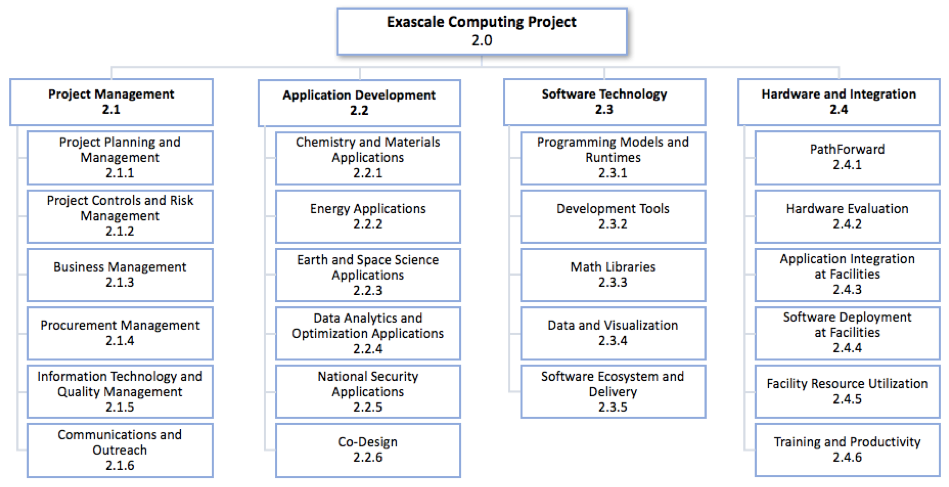
\includegraphics[width=0.9\linewidth]{ECP20}
	\caption{The ECP Work Breakdown Structure through Level 3 (L3).}
	\label{fig:ecp2}
\end{figure}

\subsection{Background}
Historically, the software used on supercomputers has come from three sources: computer system vendors, DOE laboratories, and academia. Traditionally, vendors have supplied system software:  operating system, compilers, runtime, and system-management software. The basic system software is typically augmented by software developed by the DOE HPC facilities to fill gaps or to improve management of the systems. An observation is that it is common for system software to break or not perform well when there is a jump in the scale of the system.
 
Mathematical libraries and tools for supercomputers have traditionally been developed at DOE laboratories and universities and ported to the new computer architectures when they are deployed. These math libraries and tools have been remarkably robust and have supplied some of the most impactful improvements in application performance and productivity. The challenges have been the constant adapting and tuning to rapidly changing architectures.
 
Programming paradigms and the associated programming environments that include compilers, debuggers, message passing, and associated runtimes have traditionally been developed by vendors, DOE laboratories, and universities. The same can be said for file system and storage software. An observation is that the vendor is ultimately responsible for providing a programming environment and file system with the supercomputer, but there is often a struggle to get the vendors to support software developed by others or to invest in new ideas that have few or no users yet. Another observation is that file-system software plays a key role in overall system resilience, and the difficulty of making the file-system software resilient has grown nonlinearly with the scale and complexity of the supercomputers.
 
In addition to the lessons learned from the traditional approaches, Exascale computers pose unique software challenges including the following.
\begin{itemize}
\item \textbf{Extreme parallelism:} Experience has shown that software breaks at each shift in scale. Exascale systems are predicted to have a billion-way concurrency via a combination of tasks, threads and vectorization, and more than one hundred thousand nodes. Because clock speeds have essentially stalled, the 1000-fold increase in potential performance going from Petascale to Exascale is entirely from concurrency improvements.
\item \textbf{Data movement in a deep memory hierarchy: }Data movement has been identified as a key impediment to performance and power consumption. Exascale system designs are increasing the types and layers of memory, which further challenges the software to increase data locality and reuse, while reducing data movement.
\item \textbf{Resilience:} As hardware resilience decreases due to the number of components and reduced voltage, software resilience must be developed to take up the slack and allow the Exascale system to be adaptable to component failures without the entire system crashing.  Initial concerns about resilience at the start of Exascale efforts have diminished, and the availability of non-volatile memory should dramatically improve checkpoint/restart performance.  Even so, we need to keep a focus on this issue.
\item \textbf{Power consumption:} Exascale systems have been given an aggressive power consumption goal of 20-30 MW, not much more than the power consumed by the largest systems of today. Meeting this goal will require the development of power monitoring and management software that does not exist today.
\end{itemize}
 
In addition to the software challenges imposed by the scale of Exascale computers, the following additional requirements push ECP away from the historical approaches for getting the needed software for DOE supercomputers.
\begin{itemize}
\item \textbf{2021 acceleration:} ECP has a goal of accelerating the development of the U.S. Exascale systems and enabling the first deployment by 2021. This means that the software needs to be ready sooner, and the approach of just waiting until it is ready will not work. A concerted plan that accelerates the development of the highest priority and most impactful software is needed.
\item \textbf{Productivity:} Traditional supercomputer software requires a great deal of expertise to use. ECP has a goal of making Exascale computing accessible to a wider science community than previous supercomputers have been. This requires the development of software that improves productivity and ease of use.
\item \textbf{Diversity:} There is a strong push to make software run across diverse Exascale systems. Traditionally, there has been a focus on just one new supercomputer every couple of years. ECP has a goal of enabling at least two diverse architectures, and the ECP-developed software needs to be able to run efficiently on all of them.  Some code divergence is inevitable, but careful software design, and the use of performance portability layers can minimize the amount of code targeted at a specific platform.
\item \textbf{Analytics and machine learning:} Future DOE supercomputers will need to solve emerging data science and machine learning problems in addition to the traditional modeling and simulation applications. This will require the development of scalable, parallel analytics and machine learning software that does not exist today.
\end{itemize}
 
The next section describes the approach employed by ECP ST to address the Exascale challenges.

\subsection{ECP Software Technology Approach}
ECP is taking an approach of codesign across all its principal technical areas: applications development (AD), software technology (ST), and hardware \& integration (HI). For ECP ST, this means its requirements are based on input from other areas, and there is a tight integration of the software products both within the software stack as well as with applications and the evolving hardware. 

The portfolio of projects in ECP ST is intended to address the Exascale challenges and requirements described above. We note that ECP is not developing the entire software stack for an Exascale system. For example, we expect vendors to provide the core software that comes with the system (in many cases, by leveraging ECP and other open-source efforts). Examples of vendor-provided software include operating system, file system, compilers (for C, C++, Fortran, etc.), basic math libraries, system monitoring tools, scheduler, debuggers, vendor’s performance tools, MPI (based on ECP-funded projects), OpenMP (with features from ECP-funded project), and data-centric stack components. ECP develops other, mostly higher-level software that is needed by applications and is not vendor specific. ECP-funded software activities are concerned with extreme scalability, exposing additional parallelism, unique requirements of Exascale hardware, and performance-critical components. Other software that aids in developer productivity is needed and may come from third-party open-source efforts (e.g., gdb, Valgrind).

The ST portfolio includes both ASCR and NNSA ATDM funded efforts. The MOU established between DOE-SC and NNSA has formalized this effort.  Whenever possible, ASCR and ATDM efforts are treated uniformly in ECP ST planning and assessment activities.

ST is also planning to increase integration within the ST portfolio through increased use of software components and application composition vs. monolithic application design. An important transition that ECP can accelerate is the increased development and delivery of reusable scientific software components and libraries. While math and scientific libraries have long been a successful element of the scientific software community, their use can be expanded to include other algorithms and software capabilities, so that applications can be considered more an aggregate composition of reusable components than a monolithic code that uses libraries tangentially.

To accelerate this transition, we need a greater commitment on the part of software component developers to provide reliable and portable software that users can consider to be part of the software ecosystem in much the same way users depend on MPI and compilers. At the same time, we must expect application developers to participate as clients and users of reusable components, using capabilities from components, transitioning away from (or keeping as a backup option) their own custom capabilities.

\subsubsection{The Extreme-scale Scientific Software Stack (E4S)}\label{subsubsect:e4s}
On November 8, 2018, ECP ST released version 0.1 of the Extreme-scale Scientific Software Stack, E4S (\url{http://e4s.io}).  E4S contains a collection of the software products to which ECP ST contributes.  E4S will be the primary conduit for providing easy access to ECP ST capabilities for ECP and the broader community.  E4S will also be the ECP ST vehicle for regression and integration testing across DOE pre-Exascale and Exascale systems.

\begin{figure}
		\centering
		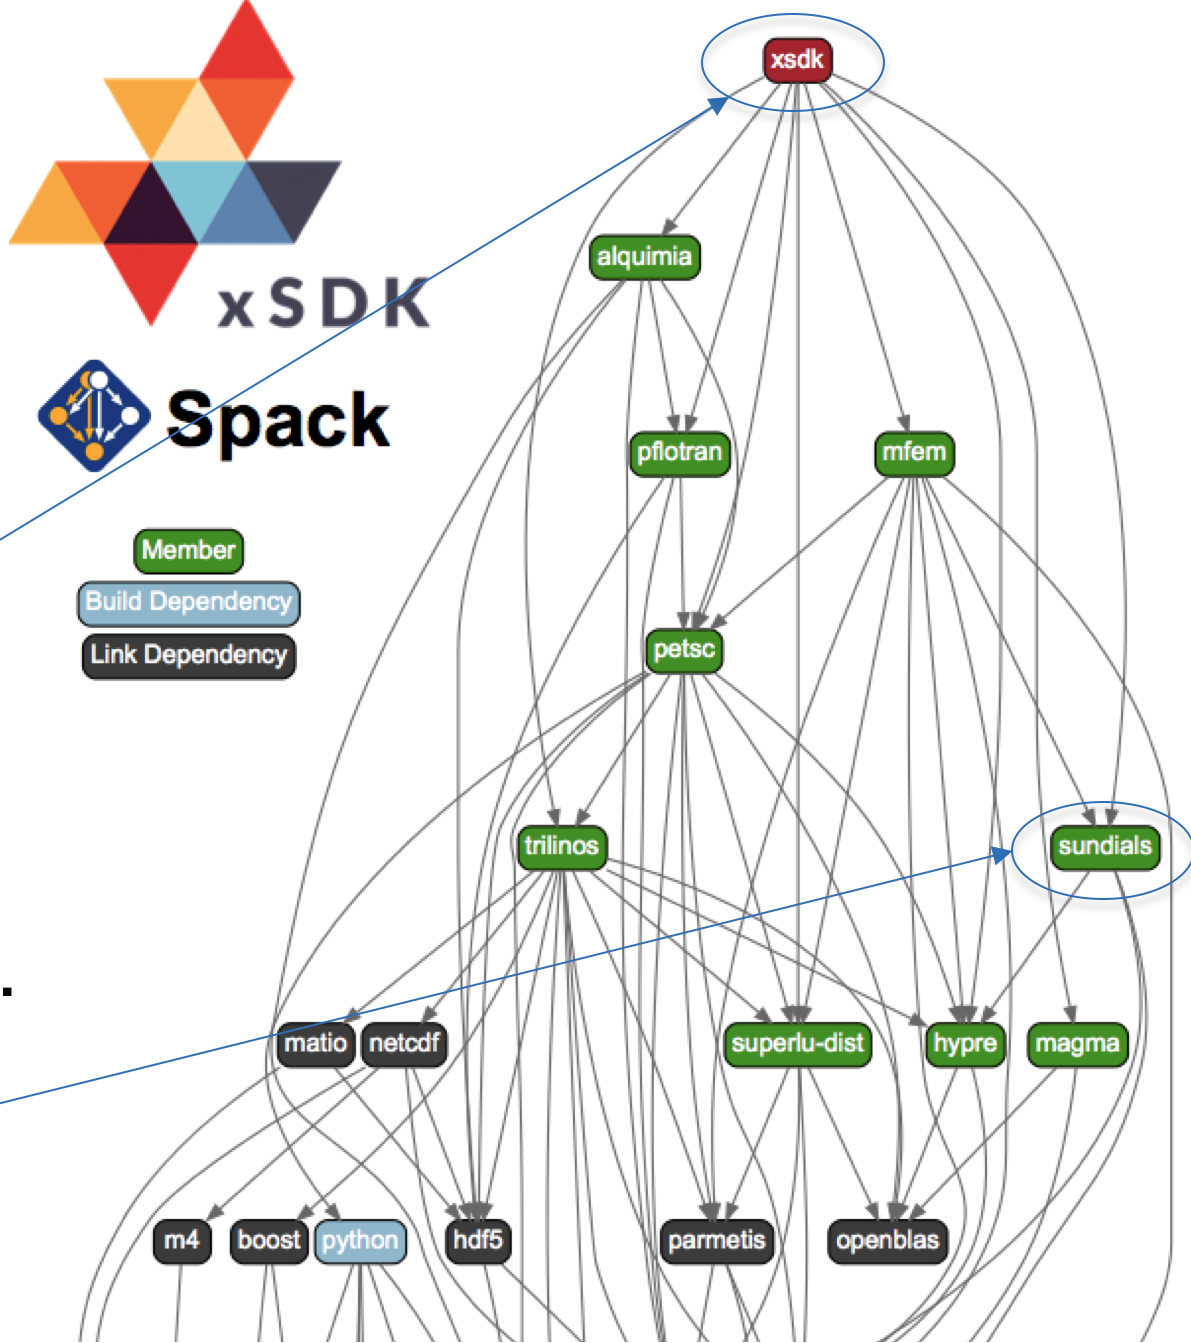
\includegraphics[scale=0.3]{E4S-Build-Tree}
	\caption{Using Spack~\cite{gamblin+:ecp18-spack-tutorial}, E4S builds a comprehensive software stack.  As ECP ST efforts proceed, we will use E4S for continuous integration testing, providing developers with rapid feedback on regression errors and providing user facilities with a stable software base as we prepare for Exascale platforms.  This diagram shows how E4S builds ECP products via an SDK target (the math libraries SDK called xSDK in this example).  The SDK target then builds all product that are part of the SDK (see Figure~\ref{fig:sdk-definition1} for SDK groupings), first defining and building external software products. Green-labeled products are part of the SDK. The blue-label indicates expected system tools, in this case a particular version of Python.  Black-labeled products are expected to be previously installed into the environment (a common requirement and easily satisified).  Using this approach, a user who is interested in only SUNDIALS (a particular math library) can be assured that the SUNDIALS build will be possible since it is a portion of what E4S builds and tests.}
	\label{fig:e4s-build-tree}
\end{figure}

E4S has the following key features:
\begin{itemize}
	\item \textbf{The E4S suite is a large and growing effort to build and test a comprehensive scientific software ecosystem:} E4S V0.1 contained 25 ECP products.  E4S V0.2, release in January 2019 contained 37 ECP products and numerous additional products needed for a complete software environment.  Eventually E4S will contain all open source products to which ECP contributes, and all related products needed for a holistic environment.
	\item \textbf{E4S is not an ECP-specific software suite:}  The products in E4S represent a holistic collection of capabilities that contain the ever-growing SDK collections sponsored by ECP and all additional underlying software required to use ECP ST capabilities.  Furthermore, we expect the E4S effort to live beyond the timespan of ECP, becoming a critical element of the scientific software ecosystem.
	\item \textbf{E4S is partitionable:} E4S products are built and tested together using a tree-based hierarchical build process.  Because we build and test the entire E4S tree, users can build any subtree of interest, without building the whole stack (see Figure~\ref{fig:e4s-build-tree}).
	\item \textbf{E4S uses Spack:} The Spack~\cite{gamblin+:ecp18-spack-tutorial} meta-build tool invokes the native build process of each product, enabling quick integration of new products, including non-ECP products.
	\item \textbf{E4S is available via containers:} In addition to a build-from-source capability using Spack, E4S maintains several container environments (Docker, Singularity, Shifter, CharlieCloud) that provides the lowest barrier to use.  Container distributions dramatically reduce installation costs and provide a ready-made environment for tutorials that leverage E4S capabilities.  For example, the ECP  application project CANDLE (Cancer Deep Learning Environment) uses an E4S container to provide a turnkey tutorial execution environment.
	\item \textbf{E4S distribution:} E4S products are available at \url{http://e4s.io}.
	\item \textbf{E4S developer community resources:} Developers interested in participating in E4S can visit the E4S-Project GitHub community at \url{https://github.com/E4S-Project}.	
\end{itemize}

The E4S effort is described in further detail in Sections~\ref{subsect:ecosystem}, especially Section~\ref{subsubsect:sdks}.

\subsubsection{Software Development Kits}\label{subsubsect:sdks}
One opportunity for a large software ecosystem project such as ECP ST is to foster increased collaboration, integration and interoperability among its funded efforts. Part of ECP ST design is the creation of software development kits (SDKs).  SDKs are collections of related software products (called packages) where coordination across package teams will improve usability and practices and foster community growth among teams that develop similar and complementary capabilities. SDKs have the following attributes:
\begin{table}
	\begin{mdframed}
\begin{enumerate}
	\item \textbf{Domain scope:} Each SDK will be composed of packages whose capabilities are within a natural functionality domain. Packages within an SDK provide similar capabilities that can enable leveraging of common requirements, design, testing and similar activities. Packages may have a tight complementary such that ready composability is valuable to the user.
	\item \textbf{Interaction models:} How packages within an SDK interact with each other. Interactions include common data infrastructure, or seamless integration of other data infrastructures; access to capabilities from one package for use in another.
	\item \textbf{Community policies:} Expectations for how package teams will conduct activities, the services they provide, software standards they follow, and other practices that can be commonly expected from a package in the SDK.
	\item \textbf{Meta-build system:} Robust tools and processes to build (from source), install and test the SDK with compatible versions of each package. This system sits on top of the existing build, install and test capabilities for each package.
	\item \textbf{Coordinated plans:} Development plans for each package will include efforts to improve SDK capabilities and lead to better integration and interoperability.
	\item \textbf{Community outreach:} Efforts to reach out to the user and client communities will include explicit focus on SDK as product suite.
\end{enumerate}
	\end{mdframed}
\caption{\label{table:sdk-attributes} Software Development Kits (SDKs) provide an aggregation of software products that have complementary or similar attributes.  ECP ST uses SDKs to better assure product interoperability and compatibility.  SDKs are also essential aggregation points for coordinated planning and testing. SDKs are an integral element of ECP ST~\cite{Heroux-SDK-Podcast}.  Section~\ref{subsubsect:ecosystem-sdk} describes the six SDK groupings and the current status of the SDK effort.}
\end{table}

\paragraph{ECP ST SDKs}
As part of the delivery of ECP ST capabilities, we will establish and grow a collection of SDKs. The new layer of aggregation that SDKs represent are important for improving all aspects of product development and delivery. The communities that will emerge from SDK efforts will lead to better collaboration and higher quality products. Established community policies will provide a means to grow SDKs beyond ECP to include any relevant external effort. The meta-build systems (based on Spack) will play an important role in managing the complexity of building the ECP ST software stack, by providing a new layer where versioning, consistency and build options management can be addressed at a mid-scope, below the global build of ECP ST products.
Each ECP ST L3 (five of them) has funds for an SDK project from which we have identified a total of six SDKs and an at-large collection of remaining products that will be delivered outside of the SDK grouping.  Section~\ref{subsubsect:ecosystem-sdk} provides an update on the progress in defining SDK groupings. For visibility, we provide the same diagram in Figure~\ref{fig:sdk-definition1-0}.

\begin{figure}[htb]
	\centering
	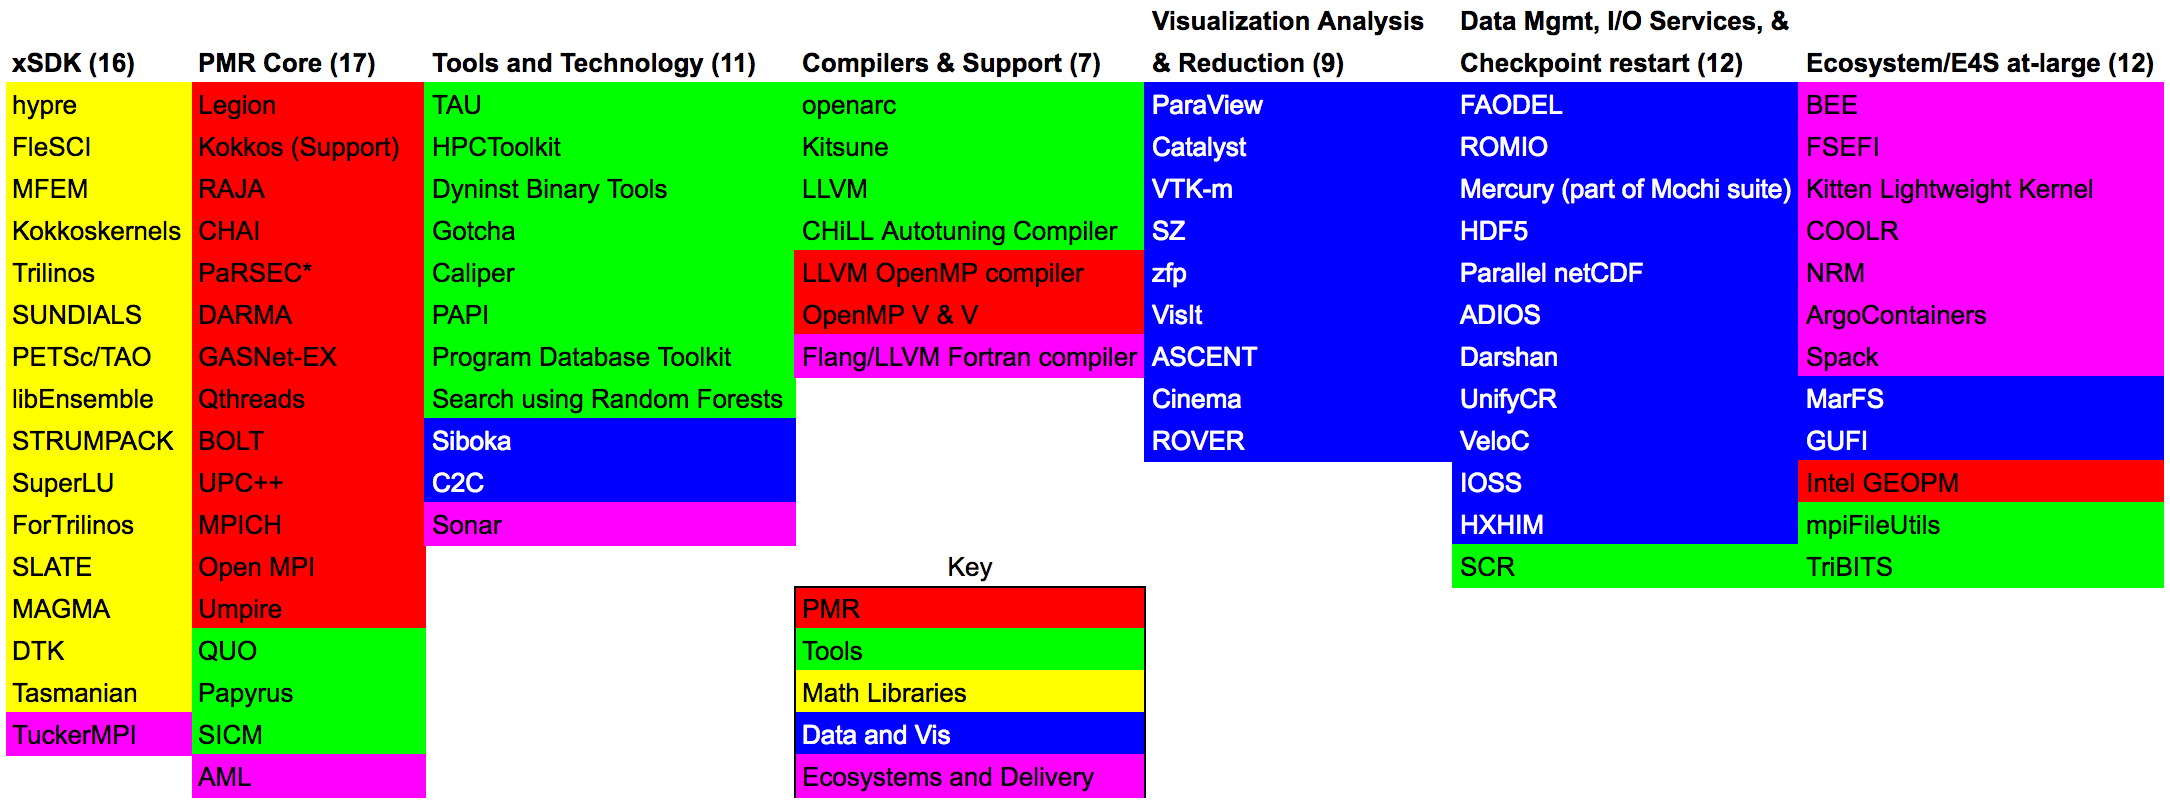
\includegraphics[width=6.5in]{projects/2.3.5-Ecosystem/2.3.5.01-Ecosystem-SDK/SDKdefinition1}
	\caption{\label{fig:sdk-definition1-0}The above graphic shows the breakdown of ECP ST products into 6 SDKs ( the first six columns).  The rightmost column lists products that are not part of an SDK, but are part of Ecosystem group that will also be delivered as part of E4S. The colors denoted in the key map all of the ST products to the ST technical area they are part of.  For example, the xSDK consists of products that are in the Math Libraries Technical area, plus TuckerMPI which is in the Ecosystem and Delivery technical area.  Section~\ref{subsubsect:ecosystem-sdk} provides an update on the progress in defining SDK groupings.}
\end{figure}


%will identify and establish at least one SDK effort. Fortunately, we will be able to leverage an existing SDK in the Math Libraries sub-element to inform our broader efforts. This SDK, called the xSDK, has been in existence for several years and has proven the value of an SDK approach in its domain (Figure~\ref{fig:xsdk-diagram}). 

%\begin{figure}
%	\centering
%	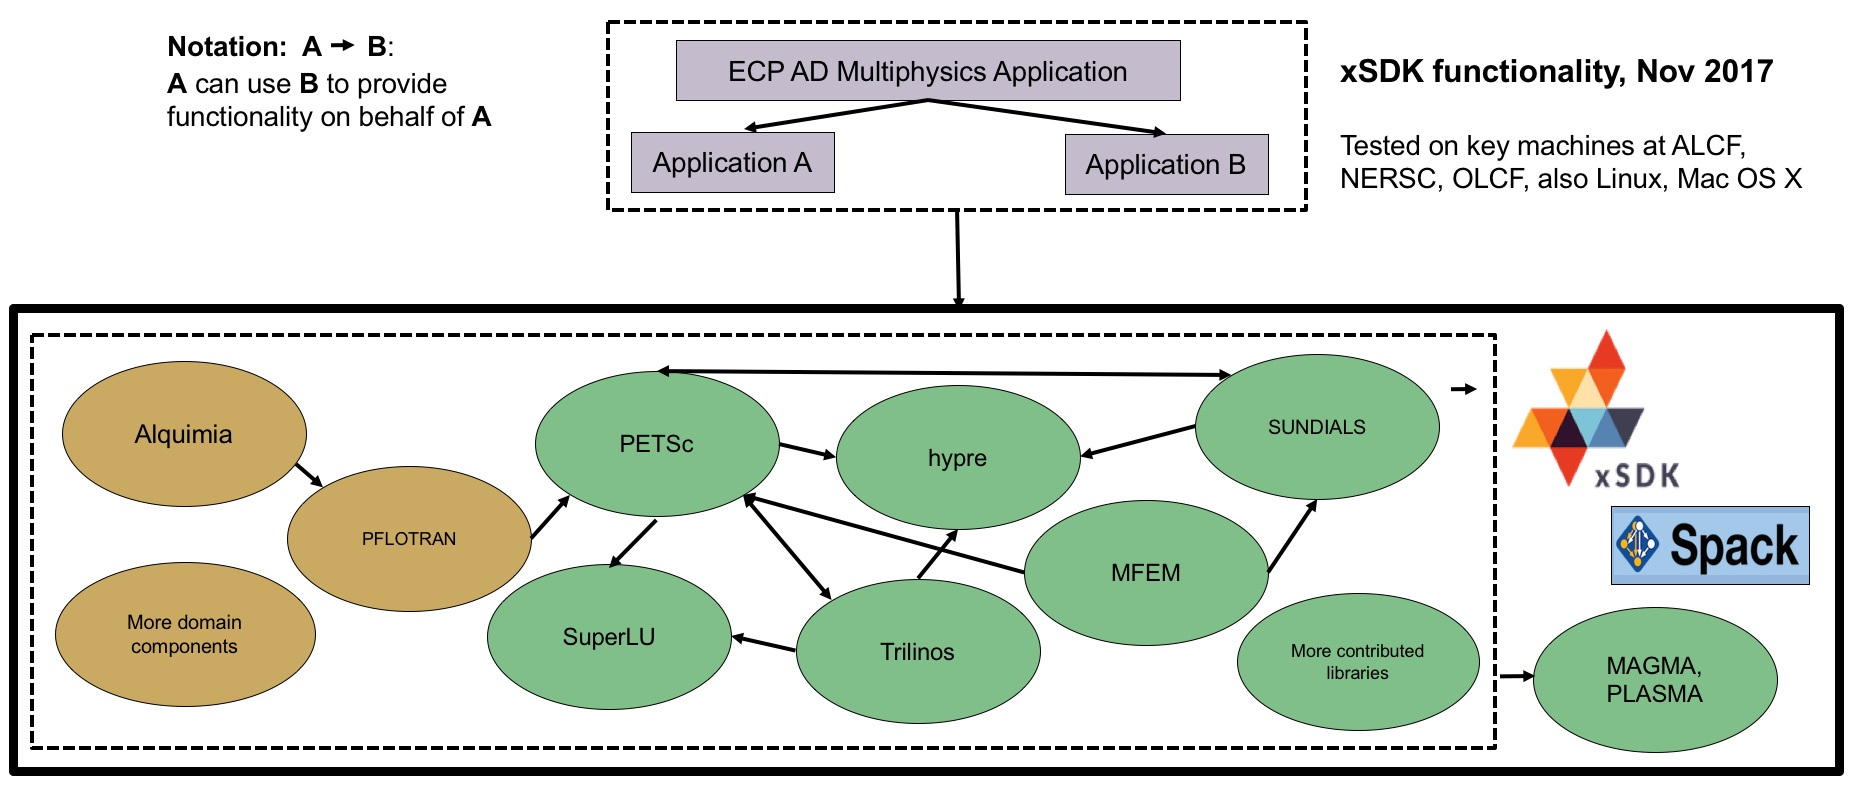
\includegraphics[width=0.9\linewidth]{xSDK-Diagram}
%	\caption{The xSDK is the first SDK for ECP ST, in the Mathematical Libraries technical area~\ref{table:wbs}. The xSDK provides the collaboration environment for improving build, install and testing capabilities for member packages such as hypre, PETSc, SuperLU and Trilinos (and other products with green background). Domain components (see orange ovals) are also an important category of the ecosystem, providing leveraged investments for common components in a specific scientific software domain.  xSDK capabilities are essential for supporting the multi-physics and multi-scale application requirement that lead to combined use of xSDK libraries. Furthermore, the availability of advanced software platforms such as GitHub, Confluence, JIRA and others enable the level of collaboration needed to create an SDK from independently developed packages.}
%	\label{fig:xsdk-diagram}
%\end{figure}
%
%
%\paragraph{The xSDK}
%Initially funded by the DOE Office of Advanced Scientific Computing Research and the office of Biological and Environmental Research as part of the IDEAS Project~\cite{Bartlett:2017:XFT:3148208.3148212}, the xSDK is a collection of independent math library packages, initially the popular libraries hypre, PETSc, SuperLU and Trilinos. The xSDK was established in recognition that collaboration across independent library development efforts could have a tremendous positive impact on the math libraries capabilities provided to users, and the productivity of library developers and sustainability of library software.
%Figure~\ref{fig:xsdk-diagram} illustrates the scope and interaction of xSDK packages and Figure~\ref{fig:xsdk-policies} lists the community policies that govern xSDK activities and set expectations for future xSDK members. While we recognize that xSDK experiences cannot be blindly applied to creation of new SDKs in ECP, the xSDK does provide a concrete, working example to guide ECP ST SDK efforts going forward.
%\begin{figure}
%	\centering
%	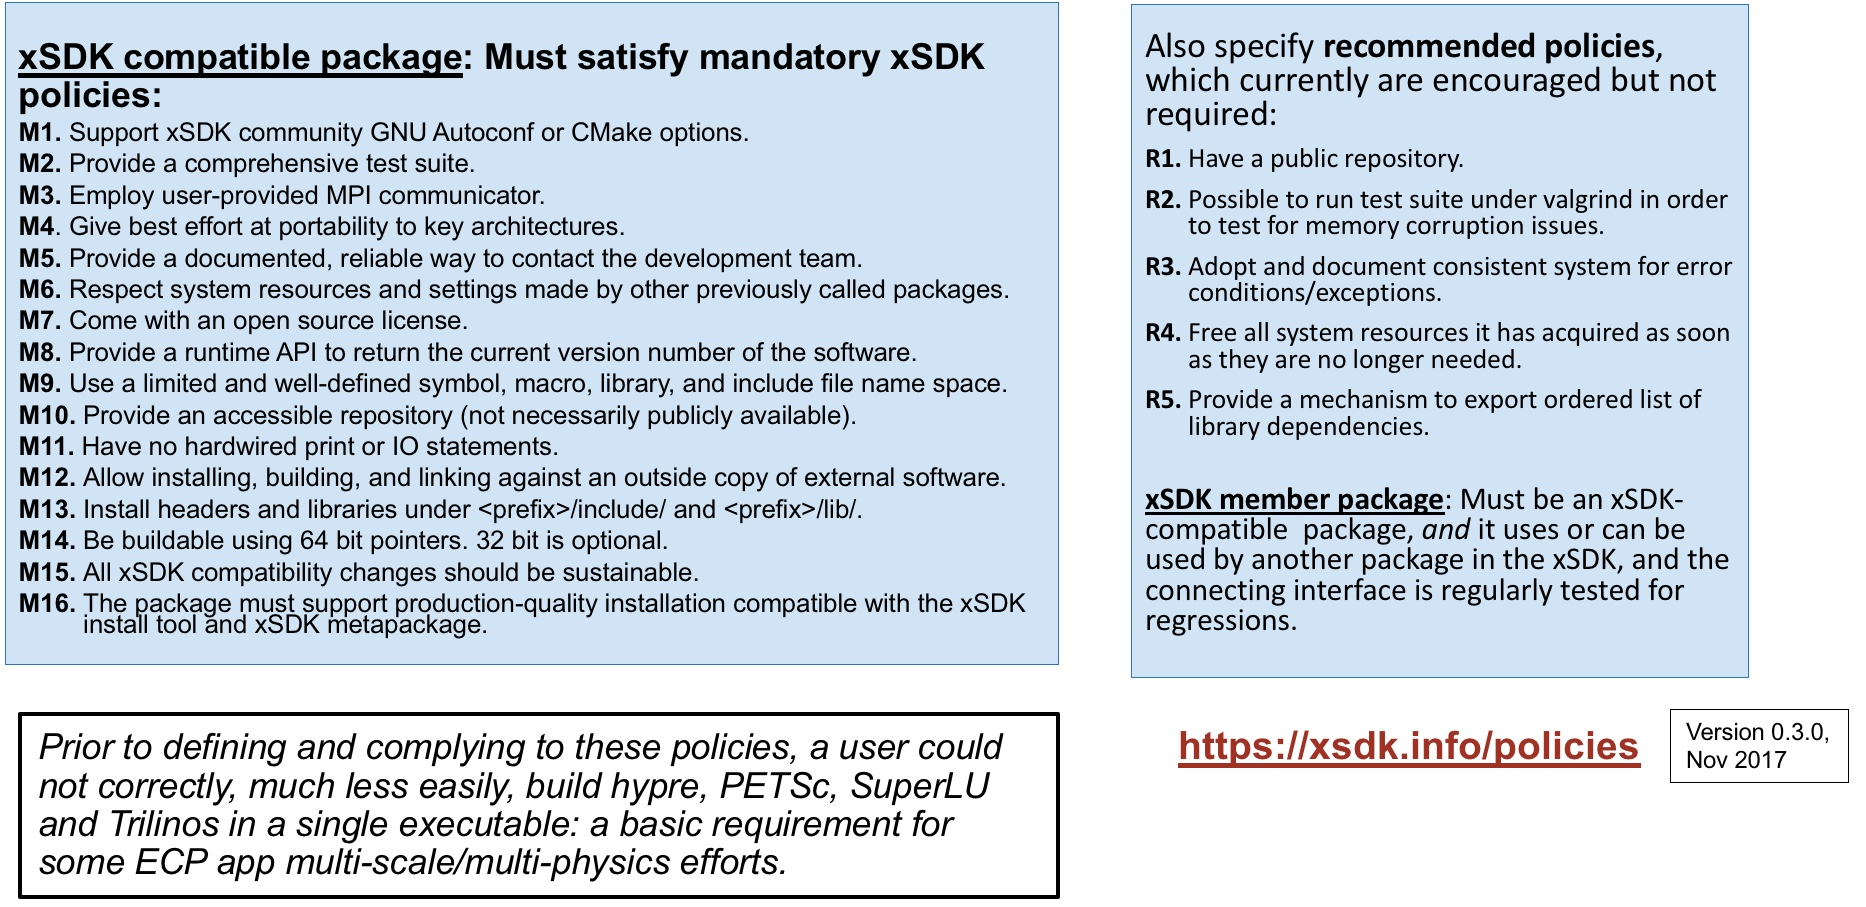
\includegraphics[width=0.9\linewidth]{xSDK-Policies}
%	\caption{\textbf{xSDK Community Policies emerged from challenging and passionate discussions about essential values of the math libraries community.} Once established, these community policies represent a living statement of what it means to be part of an SDK, and are used as the criteria for welcoming future members.}
%	\label{fig:xsdk-policies}
%\end{figure}

\subsubsection{ECP ST Software Delivery}
An essential activity for, and the ultimate purpose of, ECP ST is the delivery of a software stack that enables productive and sustainable Exascale computing capabilities for target ECP applications and platforms, and the broader high-performance computing community. The ECP ST Software Ecosystem and Delivery sub-element (WBS 2.3.5) and the SDKs in each other sub-element provide the means by which ECP ST will deliver its capabilities.
\paragraph{ECP ST Delivery and HI Deployment}
Providing the ECP ST software stack to ECP applications requires coordination between ECP ST and ECP HI. The focus areas have a complementary arrangement where ECP ST delivers its products and ECP HI deploys them. Specifically:
\begin{itemize}
	\item ST \textbf{delivers} software.  ECP ST products are delivered directly to application teams, to vendors and to facilities.  ECP ST designs and implements products to run on DOE computing facilities platforms and make products available as source code via GitHub, GitLab or some other accessible repository.
	\item HI facilitates efforts to \textbf{deploy} ST (and other) software on Facilities platforms by installing it where users expect to find it. This could be in /usr/local/bin or similar directory, or available via “module load”.
\end{itemize}
Separating the concerns of delivery and deployment is essential because these activities require different skill sets. Furthermore, ECP ST delivers its capabilities to an audience that is beyond the scope of specific Facilities’ platforms. This broad scope is essential for the sustainability of ECP ST products, expanding the user and developer communities needed for vitality. In addition, ECP HI, the computer system vendors and other parties provide deployable software outside the scope of ECP ST, therefore having the critical mass of skills to deploy the entire software stack.

\paragraph{ECP ST Delivery Strategy}
ECP ST delivers it software products as source code, primarily in repositories found on GitHub, Gitlab installations or similar platforms. Clients such as ECP HI, OpenHPC and application developers with direct repository access then take the source and build, install and test our software. The delivery strategy is outlined in Figure~\ref{fig:softwarestack}.  

Users access ECP ST products using these basic mechanisms (see Figure~\ref{fig:productsoverview} for deliverable statistics):
\begin{itemize}
	\item \textbf{Build from source code:} The vast majority of ECP ST products reach at least some of their user base via direct source code download from the product repository.  In some cases, the user will download a single compressed file containing product source, then expand the file to expose the collection of source and build files.  Increasingly, users will fork a new copy of an online repository.  After obtaining the source, the user executes a configuration process that detects local compilers and libraries and then builds the product.  This kind of access can represent a barrier for some users, since the user needs to build the product and can encounter a variety of challenges in that process, such as an incompatible compiler or a missing third-party library that must first be installed.  However, building from source can be a preferred approach for users who want control over compiler settings, or want to adapt how the product is used, for example, turning on or off optional features, or creating adaptations that extend product capabilities.  For example, large library frameworks such as PETSc and Trilinos have many tunable features that can benefit from the user building from source code.  Furthermore, these frameworks support user-defined functional extensions that are easier to support when the user builds the product from source.  ECP ST is leveraging and contributing to the development of Spack~\cite{gamblin+:sc15}.  Via meta-data stored in a Spack \textit{package} defined for each product, Spack leverages a product's native build environment, along with knowledge about its dependencies, to build the product and dependencies from source.  Spack plays a central role in ECP ST software development and delivery processes by supporting turnkey builds of the ECP ST software stack for the purposes of continuous integration testing, installation and seamless multi-product builds.
	\item \textbf{DOE computing facilities:} Each DOE computing facility (ALCF, OLCF, NERSC, LLNL and ACES [LANL/SNL]) provides pre-built versions of 17 to 20 ECP ST products (although the exact mix of products varies somewhat at each site).  Many of these products are what users would consider to be part of the core system capabilities, including compilers, e.g., Flang (Section~\ref{subsubsect:flang}) and LLVM (Section~\ref{subsubsect:sollve}), and parallel programming environments such as MPICH (Section~\ref{subsubsect:mpich}), OpenMPI (Section~\ref{subsubsect:openmpi}) and OpenMP (Section~\ref{subsubsect:bolt}).  Development tools such as PAPI (Section~\ref{subsubsect:exapapi}) and TAU (Section~\ref{subsubsect:tau}) are often part of this suite, if not already included in the vendor stack. Math and data libraries such as PETSc (Section~\ref{subsubsect:petsc}), Trilinos (Section~\ref{subsubsect:trilinos}), HDF5 (Section~\ref{subsubsect:exahdf5}) and others are also available in some facilities software installations.  We anticipate and hope for increased collaboration with facilities via the ECP Hardware \& Integration (HI) Focus Area.  We are also encouraged by multi-lab efforts such as the Tri-Lab Operating System Stack (TOSS)~\cite{TOSS} that are focused on improving uniformity of software stacks across facilities.
	\item \textbf{Vendor stacks:} Computer system vendors leverage DOE investments in compilers, tools and libraries.  Of particular note are the wide use of MPICH(Section~\ref{subsubsect:mpich}) as software base for most HPC vendor MPI implementations and the requirements, analysis, design and prototyping that ECP ST teams provide.  Section~\ref{subsection:external-contributions} describes some of these efforts.
	\item \textbf{Binary distributions:} Approximately 10 ECP ST products are available via binary distributions such as common Linux distributions, in particular via OpenHPC\cite{OpenHPC}.  ECP ST intends to foster growth of availability via binary distributions as an important way to increase the size of the user community and improve product sustainability via this broader user base.
\end{itemize}

\begin{figure}
	\centering
	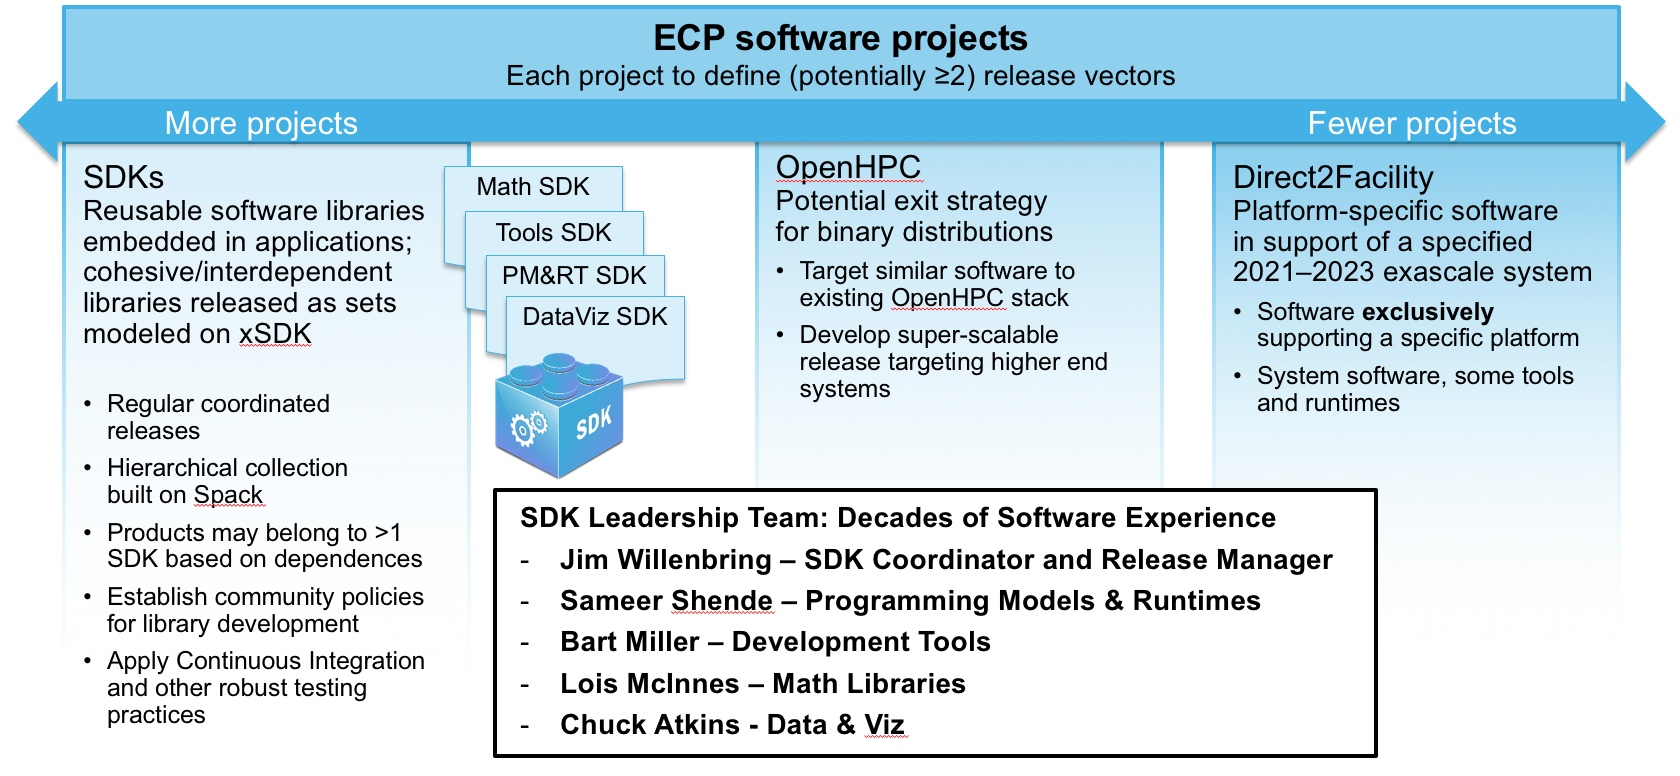
\includegraphics[width=0.9\linewidth]{SoftwareStack}
	\caption{\textbf{The ECP ST software stack is delivered to the user community through several channels.} Key channels are via source code, increasing using SDKs, direct to Facilities in collaboration with ECP HI, via binary distributions, in particular the OpenHPC project and via HPC vendors.  The SDK leadership team includes  ECP ST team members with decades of experience delivering scientific software products.}
	\label{fig:softwarestack}
\end{figure}

\subsection{ECP ST Project Restructuring}\label{subsect:ProjectRestructuring}

The initial organization of ECP ST was based on discussions that occurred over several years of Exascale planning within DOE, especially the DOE Office of Advanced Scientific Computing Research (ASCR).  Figure~\ref{fig:ecpstv1} shows the conceptual diagram of this first phase.  The 66 ECP ST projects were mapped into 8 technical areas, in some cases arbitrating where a project should go based on its primary type of work, even if other work was present in the project.  In November 2017, ECP ST was reorganized into 5 technical areas, primarily through merging a few smaller areas, and the number of projects was reduced to 56 (presently 55 due to further merging in \ecosystem).  Figure~\ref{fig:ecpstv2} shows the diagram of the second phase of ECP ST.  With the CAR V2.0, we will describe the next phase of organization refinement needed to best position ECP ST for success in the CD-2 phase of the project.

\begin{table}
\begin{tabular}{|L{1in}|L{1in}|L{1.0in}|L{2.5in}|}\hline
\textbf{WBS} & \textbf{Role/Area} & \textbf{Leader} & \textbf{Transition} \\\hline
1.3 & ECP ST Director & Rajeev Thakur & Renumbered to 2.3.  Thakur left director role, continues as lead of 2.3.1 \pmr. Mike Heroux new director. \\\hline
1.3 & ECP ST Deputy Director & Pat McCormick & McCormick left deputy role, continued as PI of 2.3.1.08 Legion project. Jonathan Carter new deputy director.\\\hline
1.3.1 & Programming Models \& Runtimes & Rajeev Thakur& Renumbered to 2.3.1, renamed to \pmr, otherwise unchanged. \\\hline
1.3.2 & Tools & Jeffrey Vetter
& Renumbered to 2.3.2, renamed to \tools, otherwise unchanged. \\\hline
1.3.3 & Math/Scientific Libs & Mike Heroux & New leader Lois Curfman McInnes, renamed Mathematical Libraries, new number 2.3.3. \\\hline
1.3.4 & Data Management \& Workflows & Rob Ross & Combined with 1.3.5 to create 2.3.4. Jim Ahrens leader. \\\hline
1.3.5 & Data Analytics \& Visualization & Jim Ahrens
& Combined with 1.3.4 to create 2.3.4. Jim Ahrens leader.\\\hline
1.3.6 & System Software & Martin Schulz& Combined with 1.3.7 and 1.3.8 into 2.3.5. Rob Neely leader.\\\hline
1.3.7 & Resilience & Al Geist & Combined with 1.3.6 and 1.3.8 into 2.3.5. Rob Neely leader. \\\hline
1.3.8 & Integration & Rob Neely & 
Combined with 1.3.6 and 1.3.7 into 2.3.5. Rob Neely leader. \\\hline
\end{tabular}
	\caption{\label{fig:wbs-transition}ECP ST technical areas were reduced from 8 to 5 in November 2017.  This figure shows how areas were remapped and merged.  In addition, the ECP ST Director and Deputy Director changed from Rajeev Thakur (who continues as the \pmr\ lead) and Pat McCormick to Mike Heroux and Jonathan Carter, respectively.}
\end{table}

\begin{figure}
\begin{mdframed}
\begin{itemize}
\item Phase 1: 66 total projects
\begin{itemize}
\item 35 projects funded by the DOE Office of Science that were selected in late 2016 via an RFI and RFP process, considering prioritized requirements of applications and DOE facilities. 
These projects started work in January–March 2017 depending on when the contracts were awarded.
\item 31 ongoing DOE NNSA funded projects that are part of the Advanced Technology Development and Mitigation (ATDM) program. The ATDM program started in FY14.  These projects are focused on longer term research to address the shift in computing technology to extreme, heterogeneous architectures and to advance the capabilities of NNSA simulation codes.
\end{itemize}
\item Phase 2: 56 total projects
(now 55 after further merging in 2.3.5)
\begin{itemize}
\item 41 ASCR-funded projects.  Added  2 \ecosystem\ projects and 4 SDK projects.
\item 15 ATDM projects: Combined the previous 31 ATDM projects into one project per technical area per lab.  ATDM projects are generally more vertically integrated and would not perfectly mapped to any proposed ECP ST technical structure.  Minimizing the number of ATDM projects within the ECP WBS structure reduces complexity of ATDM to ECP coordination and gives ATDM flexibility in revising its portfolio without disruption to the ECP-ATDM mapping.
\end{itemize}
\item Phase 3: Fewer, larger and more uniform-sized projects
\begin{itemize}
	\item Starting with FY2020, ECP ST will further consolidate L4 projects to foster additional synergies and amortize project overheads as ECP heads into Critical Decision Phase 2~\cite{413.3B}, where more rigor in planning and execution are needed.
	\item Details of this plan are available to project stakeholders in the CAR V1.5 appendix and will be in the public portion of the CAR V2.0 in July 2019.
\end{itemize}
\end{itemize}
\end{mdframed}

\caption{\label{fig:project-remapping}Project remapping summary from Phase 1 (through November 2017) to Phase 2 (After November 2017) to Phase 3 (After October 1, 2019)}
\end{figure}


\begin{figure}
	\centering
	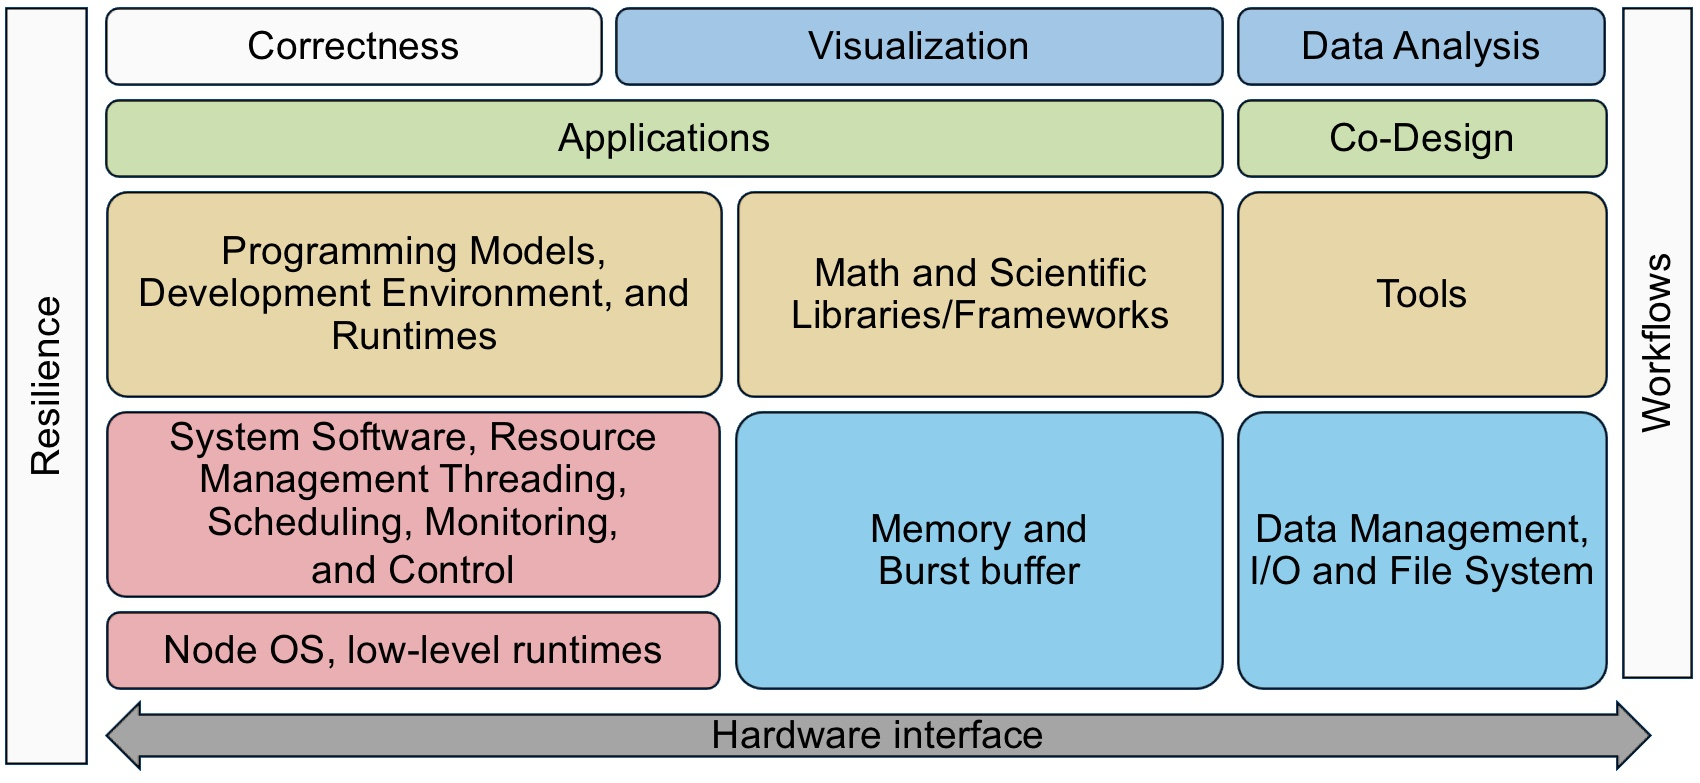
\includegraphics[width=0.9\linewidth]{ECPSTV1}
	\caption{ECP ST before November 2017 reorganization.  This conceptually layout emerged from several years of Exascale planning, conducted primarily within the DOE Office of Advanced Scientific Computing Research (ASCR).  After a significant restructuring of ECP that removed much of the facilities activities and reduced the project timeline from 10 to seven years, and a growing awareness of what risks had diminished, this diagram no longer represented ECP ST efforts accurately.}
	\label{fig:ecpstv1}
\end{figure}
\begin{figure}
	\centering
	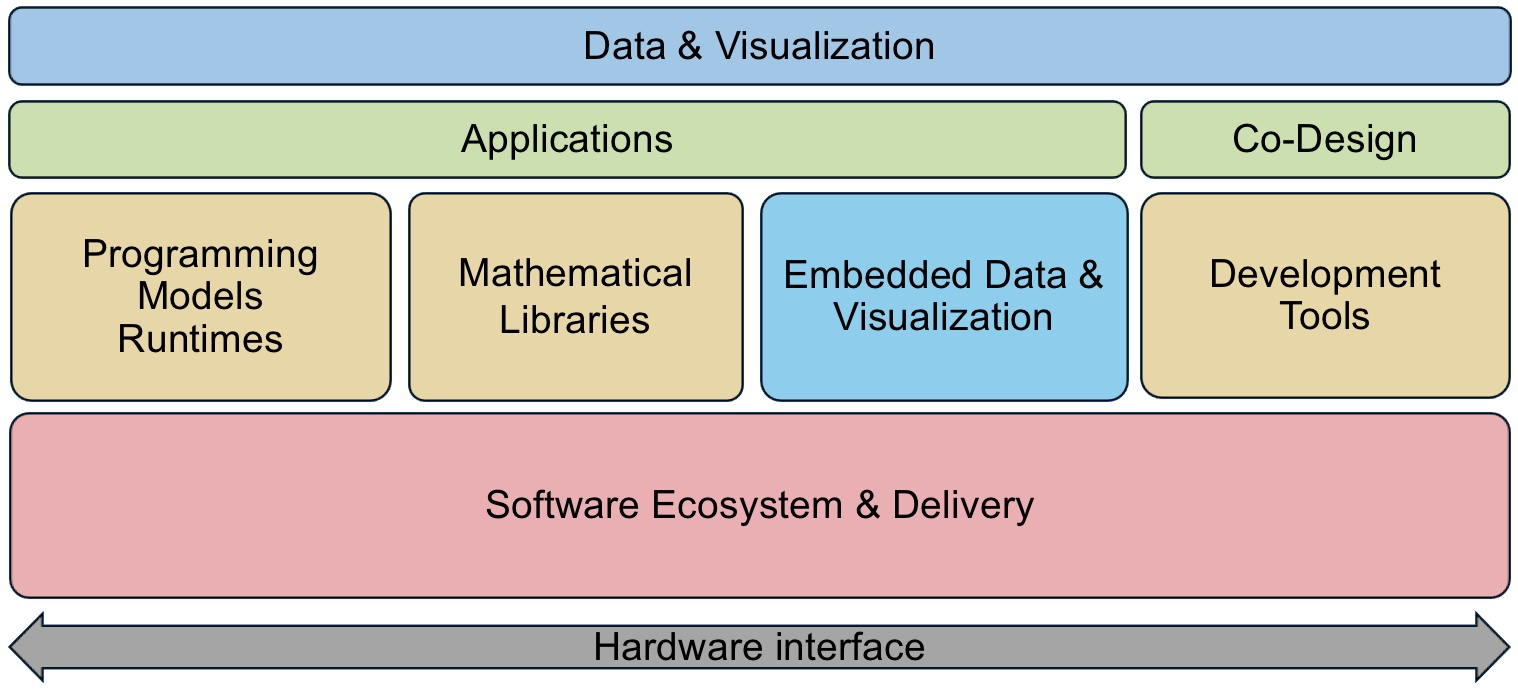
\includegraphics[width=0.9\linewidth]{ECPSTV2}
	\caption{ECP ST after November 2017 reorganization.  This diagram more accurately reflects the priorities and efforts of ECP ST given the new ECP project scope and the demands that we foresee.}
	\label{fig:ecpstv2}
\end{figure}
\begin{figure}
	\centering
	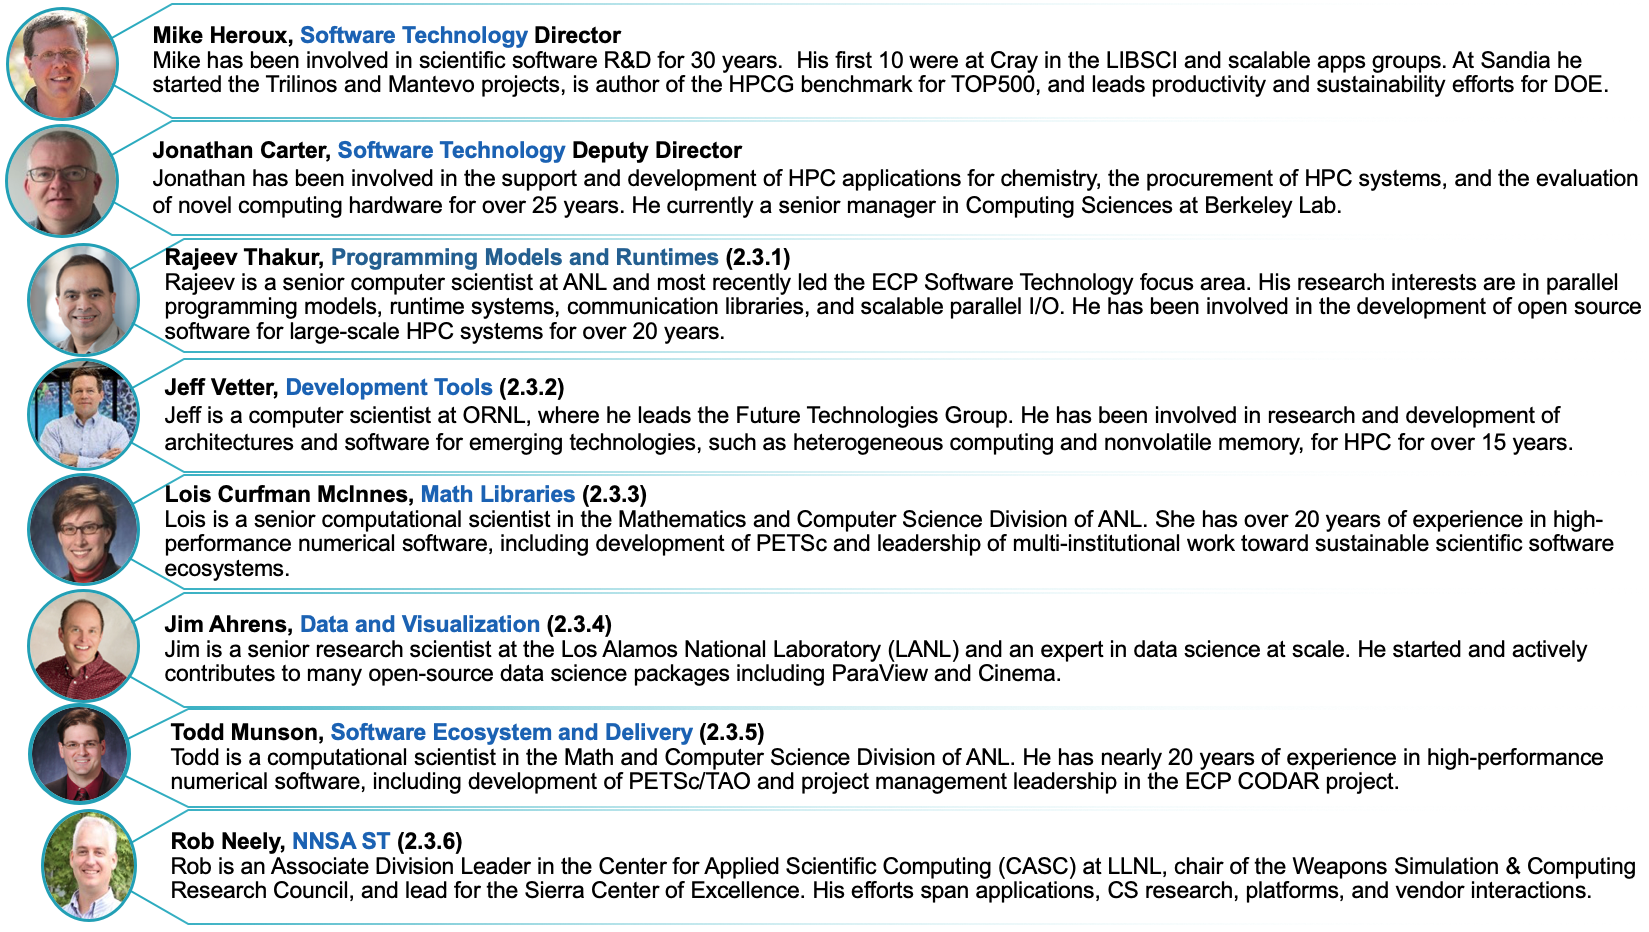
\includegraphics[width=0.9\linewidth]{ECP-ST-Leads}
	\caption{ECP ST Leadership Team as of November 2017.}
	\label{fig:ecpstleads}
\end{figure}

%\subsection{New Project Efforts}
%ECP ST is preparing several strategic changes for the FY2020 restructuring (Phase 3).   These changes will be reported in the CAR V2.0.  No other significant changes have been made since the CAR V1.0.


%\subsubsection{FFTs}\label{subsubsect:ffts}
%ECP ST has initiated two new efforts in Fast Fourier Transforms (FFTs).  FFTs provide an essential mathematical tool to many application areas.  From the very beginning of HPC, vendors have provided optimized FFT libraries for their users.  The advent of FFTW~\cite{FFTW05}, a tunable high-performance library with a well-designed interface, enabled a \textit{de facto} standardization of FFT interfaces, and an effective source base for vendor libraries, which adapted FFTW source for their platforms.
%
%There is some concern in the community that FFTW is no longer actively developed, nor well prepared for emerging platforms.  Furthermore, FFTW's strong copylefting license (which forces its users to make their own software open source in the same way) has always been a challenge to users.  While vendors are still committed to providing optimized FFT libraries, whether or not FFTW is available, we believe it is prudent to explore a new software stack and have funded a short-term project to explore this possibility.  The new library will also explore problem formulations that could significantly reduce the computational cost of FFTs.  This new effort, called FFTX, will be led by Lawrence Berkeley National Lab, under the existing math libraries project (Section~\ref{subsubsect:strumpack}).
%
%A second FFT project will address a consensus opportunity to provide a sustainable 3D FFT library built from established but \textit{ad hoc} software tools that have traditionally been part of application codes, but not extracted as independent, supported libraries.  These 3D FFTs rely on third-party 1D FFTs, either from FFTW or from vendor libraries.
%
%The goal of this second project, FFT-ECP, led by the University of Tennessee and integrated into one of its existing projects (Section~\ref{subsubsect:slate}) is to:
%\begin{itemize}
%\item Collect existing FFT capabilities recently made available from ECP application teams (LAMMPS/fftMPI and HACC/SWFFT). 
%\item Assess gaps and make available as a sustainable math library.
%\item Explore opportunities to build 3D FFT libraries on vendor 1D and 2D kernels, especially leveraging on-node concurrency from 2D and batched 1D formulations.
%\item Focus on capabilities for Exascale platforms.
%\item Emphasize leverage of vendor capabilities and addressing vendor deficiencies over creation of new and independent software stack.
%\end{itemize}
%
%This effort, while not addressing the concerns about FFTW directly, is essential to providing a new and sustainable FFT software stack that leverages the large investment by the broader HPC community in FFT software.  The payoff from this effort is almost guaranteed.  Also, should the FFTX project also go forward, it will provide an FFTW-compatible interface that would allow FFT-ECP to use FFTX as one option, in addition to external FFT libraries.
%
%\subsubsection{LLNL Math Libraries}\label{subsubsect:llnl-math-libs}
%When ECP ST started, some important capabilities were not part of the original portfolio, even though their engagement is essential for ECP application success.  This is true of the LLNL math library \textit{hypre}~\cite{hypre}.  This library is widely used to provide scalable multigrid preconditioners across several ECP applications.  Funding to support adaptation of \textit{hypre}  in preparation for Exascale platforms at science lab facilities, e.g., Argonne, and for ECP science applications was not part of the original ECP ST portfolio.  We have added funding for this effort, starting in June 2018.  In addition, we provided new funding for another LLNL math library, MFEM~\cite{mfem:homepage}, so that the MFEM team can participate in SDK efforts for math libraries.

\newpage
\section{ECP ST Technical Areas}
\subsection{\stid{1}  \pmr}

\textbf{End State:} A cross-platform, production-ready programming environment that enables and accelerates the development of mission-critical software at both the node and full-system levels.

\subsubsection{Scope and Requirements}
A programming model provides the abstract design upon which developers express and coordinate the efficient parallel execution of their program. A particular model is implemented as a developer-facing interface and a supporting set of runtime layers. To successfully address the challenges of exascale computing, these software capabilities must address the challenges of programming at both the node- and full-system levels. These two targets must be coupled to support multiple complexities expected with exascale systems (e.g., locality for deep memory hierarchies, affinity for threads of execution, load balancing) and also provide a set of mechanisms for performance portability across the range of potential and final system designs. Additionally, there must be mechanisms for the interoperability and composition of multiple implementations (e.g., one at the system level and one at the node level). This must include abilities such as resource sharing for workloads that include coupled applications, supporting libraries and frameworks, and capabilities such as in situ analysis and visualization. 

Given the ECP’s timeline, the development of new programming languages and their supporting infrastructure is infeasible. We do, however, recognize that the augmentation or extension of the features of existing and widely used languages (e.g., C/C++ and Fortran) could provide solutions for simplifying certain software development activities. 

\subsubsection{Assumptions and Feasibility}
The intent of the PMR L3 is to provide a set of programming abstractions and their supporting implementations that allow programmers to select from options that meet demands for expressiveness, performance, productivity, compatibility, and portability. It is important to note that, while these goals are obviously desirable, they must be balanced with an additional awareness that today’s methods and techniques may require changes in both the application and the overall programming environment and within the supporting software stack.

\subsubsection{Objectives}
PMR provides the software infrastructure necessary to enable and accelerate the development of HPC applications that perform well and are correct and robust, while reducing the cost both for initial development and ongoing porting and maintenance. PMR activities need to reflect the requirements of increasingly complex application scenarios, usage models, and workflows, while at the same time addressing the hardware challenges of increased levels of concurrency, data locality, power, and resilience. The software environment will support programming at multiple levels of abstraction that includes both mainstream as well as alternative approaches if feasible in ECP’s timeframe. 

Both of these approaches must provide a portability path such that a single application code can run well on multiple types of systems, or multiple generations of systems, with minimal changes. The layers of the system and programming environment implementation will therefore aim to hide the differences through compilers, runtime systems, messaging standards, shared-memory standards, and programming abstractions designed to help developers map algorithms onto the underlying hardware and schedule data motion and computation with increased automation.
\subsubsection{Plan}
PMR contains nine L4 projects. To ensure relevance to DOE missions, these efforts leverage and collaborate with existing activities within the broader HPC community. The PMR area supports the research and development needed to produce exascale-ready versions of the Message Passing Interface (MPI);  Partitioned Global-Address Space Libraries (UPC++, GASNet); task-based programming models (Legion, PaRSEC); software for node-level performance portability (Kokkos, RAJA); and libraries for memory, power, and resource management.
Initial efforts focused on identifying the core capabilities needed by the selected ECP applications and components of the software stack, identifying shortcomings of current approaches, establishing performance baselines of existing implementations on available petascale and prototype systems, and the re-implementation of the lower-level capabilities of relevant libraries and frameworks. These efforts provided demonstrations of parallel performance of algorithms on pre-exascale, leadership-class machines--at first on test problems, but eventually in actual applications (in close collaboration with the AD and HI teams). Initial efforts also informed research into exascale-specific algorithms and requirements that will be implemented across the software stack. The supported projects targeted and implemented early versions of their software on CORAL, NERSC and ACES pre-exascale systems--with an ultimate target of production-ready deployment on the exascale systems.
In FY20--23, the focus will be on development and tuning for the specific architectures of the selected exascale platforms, in addition to tuning specific features that are critical to ECP applications.

Throughout the effort, the applications teams and other elements of the software stack evaluate and provide feedback on their functionality, performance, and robustness. Progress towards these goals is documented quarterly and evaluated annually (or more frequently if needed) based on PMR-centric milestones as well as joint milestone activities shared across associated software stack activities by Application Development and Hardware \& Integration focus areas.


\subsubsection{Risks and Mitigation Strategies}
The mainstream activities of PMR focus on advancing the capabilities of the Message Passing Interface (MPI) and OpenMP. Pushing them as far as possible into the exascale era is key to supporting an evolutionary path for applications. This is the primary risk mitigation approach for both PMR and existing application codes. Extensions to MPI and OpenMP standards require research, and part of the efforts will focus on rolling these findings into existing standards, which takes time. To further address risks, PMR is exploring alternative approaches to mitigate the impact of potential limitations of the MPI and OpenMP programming models. This effort is tracked using the risk register.

Another risk is the failure of adoption of the software stack by the vendors, which is tracked in the risk register, and mitigated by the specific delivery focus in sub-element SW Ecosystems and Delivery. Past experience has shown that a combination of laboratory-supported open source software and vendor-optimized solutions built around standard APIs that encourage innovation across multiple platforms is a viable approach and what we are doing in PMR. We are using close interaction with the vendors early on to encourage adoption of the software stack, including well-tested practices of including support for key software products or APIs into large procurements through NRE or other contractual obligations. A mitigation strategy for this approach involves building a long-lasting open source community around projects that are supported via laboratory and university funding. This approach is being extended to other APIs and alternative models (that are being defined and eventually standardized) to allow for deeper and stack-wide introspection as well as resource sharing.

Creating a coordinated set of software requires strong management to ensure that duplication of effort is minimized. This is recognized by ECP management, and processes are in place to ensure collaboration is effective, shortcuts are avoided unless necessary, and an agile approach to development is instituted to prevent prototypes moving directly to product. The duplication of effort specifically, and the overall integration of the software stack, are tracked in the risk register. 

\subsubsection{Future Trends}

\subsection{\stid{2} \tools}

\textbf{End State:}	A suite of development tools and supporting unified infrastructure aimed at improving developer productivity across increasingly complex architectures, especially those targeted for Exascale platforms.


\subsubsection{Scope and Requirements}
For Exascale systems, the compilers, profilers, debuggers, and other software development tools must be increasingly sophisticated to give software developers insight into the behavior of not only the application and the underlying hardware but also the details corresponding to the underlying programming model implementation and supporting runtimes (e.g., capturing details of locality and affinity). These capabilities should be enhanced with further integration into the supporting compiler infrastructure and lower layers of the system software stack (e.g., threading, runtime systems, and data transport libraries), and hardware support. Most of the infrastructure will be released as open source, as many of them already are, with a supplementary goal of transferring the technology into commercial products. Given the diversity of Exascale systems architectures, some subset of the tools may be specific to one or more architectural features and is potentially best implemented and supported by the vendor; however, the vendor will be encouraged to use open APIs to provide portability, additional innovation, and integration into the tool suite and the overall software stack.


\subsubsection{Assumptions and Feasibility }

The overarching goal of improving developer productivity for Exascale platforms introduces new issues of scale that will require more lightweight methods, hierarchical approaches, and improved techniques to guide the developer in understanding the characteristics of their applications and to discover sources of the errors and performance issues. Additional efforts for both static and dynamic analysis tools to help identify lurking bugs in a program, such as race conditions, are also likely needed. The suite of needed capabilities spans interfaces to hardware-centric resources (e.g., hardware counters, interconnects, and memory hierarchies) to a scalable infrastructure that can collect, organize, and distill data to help identify performance bottlenecks and transform them into an actionable set of steps and information for the software developer. Therefore, these tools share significant challenges due to the increase in data and the resulting issues with management, storage, selection, analysis, and interactive data exploration. This increased data volume stems from multiple sources, including increased concurrency, processor counts, additional hardware sensors and counters on the systems, and increasing complexity in application codes and workflows.

Compilers obviously play a fundamental role in the overall programming environment but can also serve as a powerful entry point for the overall tool infrastructure. In addition to optimizations and performance profiling, compiler-based tools can help with aspects of correctness, establishing connections between programming model implementations and the underlying runtime infrastructures, and auto-tuning. In many cases, today's compiler infrastructure is proprietary and closed source, limiting the amount of flexibility for integration and exploration into the Exascale development environment. In addition to vendor compiler options, this project aims to provide an open source compiler capability that can play a role in better supporting and addressing the challenges of programming at Exascale. 


\subsubsection{Objectives}

This project will design, develop, and deploy an Exascale suite of development tools built on a unified infrastructure for development, analysis, and optimization of applications, libraries, and infrastructure from the programming environments of the project. The overarching goal is to leverage and integrate the data measurement, acquisition, storage, and analysis and visualization techniques being developed in other projects of the software stack. The project will seek to leverage techniques for common and identified problem patterns and create new techniques for data exploration related to profiling and debugging and support advanced techniques such as autotuning and compiler integration. We will seek to establish an open-source compiler activity leveraging activities around the LLVM infrastructure. These efforts will require collaboration and integration with system monitoring and various layers within the software stack.


\subsubsection{Plan}
It is expected that multiple projects will be supported under the tools effort. To ensure relevance to DOE missions, most of these efforts shall be DOE laboratory led and leverage and collaborate with existing activities within the broader HPC community. Initial efforts will focus on identifying the core capabilities needed by the selected ECP applications, components of the software stack, expected hardware features, and the selected industry activities from within the Hardware and Integration focus area. The supported projects will target and implement early versions of their software on both CORAL and APEX systems, with an ultimate target of production-ready deployment on the Exascale systems. Throughout this effort the applications teams and other elements of the software stack will evaluate and provide feedback on their functionality, performance, and robustness. These goals will be evaluated yearly (or more often as needed) based on milestones as well as joint milestone activities shared across the associated software stack activities by AD and HI focus areas.

\subsubsection{Risks and Mitigations Strategies}

A risk exists in terms of adoption of the various tools and their supporting infrastructure by the broader community, including support by system vendors. Past experience has shown that a combination of laboratory-supported open source software and vendor-optimized solutions built around standard APIs that encourage innovation across multiple platforms is a viable approach, and this will be undertaken. We will track this risk primarily via the risk register.

Given its wide use within a range of different communities, and its modular design principles, the project's open source compiler activities will focus on the use of the LLVM compiler infrastructure as a path to reduce both scope and complexity risks and leverage with an already established path for NRE investments across multiple vendors. The compilers and their effectiveness are tracked in the risk register. 

Another major risk for projects in this area is the lack of low-level access to hardware and software necessary for using emerging architectural features. Many of these nascent architectural features have immature implementations and software interfaces that must be refined prior to release to the broader community. This project should be at the forefront of this interaction with early delivery systems. This risk is also tracked in the risk register for compilers, which are particularly vulnerable.


\subsection{\stid{3} \mathlibs}

\textbf{End State:} Mathematical libraries that (i) interoperate with the ECP software stack; (ii) are incorporated into the ECP applications; and (iii) provide scalable, resilient numerical algorithms that facilitate efficient simulations on Exascale computers.

\subsubsection{Scope and Requirements}
Software libraries are powerful means of sharing verified, optimized algorithms and their implementations. Applied research, development, and support are needed to extend existing DOE mathematical software libraries to make better use of Exascale architectural features. DOE-supported libraries encapsulate the latest results from mathematics and computer science R\&D; many DOE mission-critical applications rely on these numerical libraries and frameworks to incorporate the most advanced technologies available. 

The Mathematical Libraries effort will ensure the healthy functionality of the numerical software libraries on which the ECP applications will depend. The DOE mathematical software libraries used by computational science and engineering applications span the range from light-weight collections of subroutines with simple APIs to more “end-to-end” integrated environments and provide access to a wide range of algorithms for complex problems.

Advances in mathematical and scientific libraries will be necessary to enable computational science on Exascale systems. Exascale computing promises not only to provide more computational resources enabling higher-fidelity simulations and more demanding studies but also to enable the community to pose new scientific questions. Exascale architectural characteristics introduce new features that algorithms and their implementations will need to address in order to be scalable, efficient, and robust. As a result, it will be necessary to conduct research and development to rethink, reformulate, and develop existing and new methods and deploy them in libraries that can be used by applications to deliver more complete and sophisticated models and provide enhanced predictive simulation and analysis capabilities.

The Mathematical Libraries effort must (1) collaborate closely with the Application Development effort (WBS 2.2) to be responsive to the needs of the applications and (2) collaborate with the other products within the Software Technology effort (WBS 2.3) in order to incorporate new technologies and to provide requirements. All software developed within the Mathematical Libraries effort must conform to best practices in software engineering, which will be formulated early in the project in collaboration with the Applications Development focus area. Software produced by this effort must provide scalable numerical algorithms that enable the application efforts to reach their performance goals, encapsulated in libraries whose data structures and routines can be used to build application software.

\subsubsection{Assumptions and Feasibility}
Years of DOE investment have led to a diverse and complementary collection of mathematical software, including AMReX, Chombo, hypre, Dakota, DTK, MAGMA, MFEM, PETSc/TAO, PLASMA, ScaLAPACK, SUNDIALS, SuperLU, and Trilinos. This effort is evolving a subset of existing libraries to be performant on Exascale architectures. In addition, research and development is needed into new algorithms whose benefits may be seen only at the extreme scale. Results of preliminary R\&D projects indicate that this approach is feasible.

Additionally, ECP will need to rely on a strong, diverse, and persistent base math research program, which is assumed to continue being supported by the DOE-SC ASCR Office. The ECP technical directors will schedule quarterly meetings with the ASCR research program managers to get updates on research results that might meet ECP requirements as well as to inform the program managers of ECP needs in applications and software components.

\subsubsection{Objectives}
The high-level objective of the Mathematical Libraries effort is to provide scalable, resilient numerical algorithms that facilitate efficient application simulations on Exascale computers. To the greatest extent possible, this objective should be accomplished by preserving the existing capabilities in mathematical software while evolving the implementations to run effectively on the Exascale systems and adding new capabilities that may be needed by Exascale applications.

The key performance metrics for the software developed by this effort are scalability, efficiency, and resilience. As a result of the new capabilities in mathematics libraries developed under this effort, applications will tackle problems that were previously intractable and will model phenomena in physical regimes that were previously unreachable.

\subsubsection{Plan}
As detailed below, the Mathematical Libraries effort supports six complementary L4 projects as needed to meet the needs of ECP applications. These efforts include strong collaborations among DOE labs, academia, industry, and other organizations, and leveraging existing libraries that are widely used by the DOE HPC community. 

Initial efforts have focused on identifying core capabilities needed by selected ECP applications, establishing performance baselines of existing implementations on available Petascale and prototype systems, and beginning re-implementation of lower-level capabilities of the libraries and frameworks. Another key activity is collaborating across all projects in the Mathematical Libraries effort to define community policies in order to enable compatibility among complementary software and to provide a foundation for future work on deeper levels of interoperability. Refactoring of higher-level capabilities will be prioritized based on needs of the applications. In time, these efforts will provide demonstrations of parallel performance of algorithms from the mathematical software on pre-Exascale, leadership-class machines (at first on test problems, but eventually in actual applications). The initial efforts also are informing research into advanced exascale-specific numerical algorithms that will be implemented within the libraries and frameworks. In FY20–23, the focus will be on development and tuning for the specific architectures of the selected exascale platforms, in addition to tuning specific features that are critical to ECP applications. The projects will implement their software on the CORAL, NERSC and ACES systems, and ultimately on initial Exascale systems, so that functionality, performance, and robustness can be evaluated by the applications teams and other elements of the software stack. Throughout the effort the applications teams and other elements of the software stack will evaluate and provide feedback on their functionality, performance, and robustness. These goals will be evaluated at least yearly based on milestones as well as joint milestone activities shared across the associated software stack activities by Application Development and Hardware and Integration project focus areas.


\subsubsection{Risks and Mitigations Strategies}
There are a number of foreseeable risks associated with the Mathematical Libraries effort.
\begin{itemize}
	\item Efficient implementation of new or refactored algorithms to meet Exascale computing requirements may introduce unanticipated requirements on programming environments. To mitigate this risk, effective communication is needed between projects in the Mathematical Libraries effort and projects tasked with developing the programming environments. From the application perspective, this is specifically tracked in a specific AD risk the risk register. Additionally, the risks of an inadequate programming environment overall are tracked as a specific ST risk in the risk register.
	\item A significant number of existing algorithms currently implemented in numerical libraries may scale poorly, thereby requiring significantly more effort than refactoring. The R\&D planned for the first three years of the ECP is the first mitigation for this risk (as well as the co-design centers planned in Application Development). In addition, the ECP will be able to draw from a strong, diverse, well-run, persistent base math research program. From the application perspective, this is tracked via an AD risk in the risk register. Scaling issues for the software stack in general, including libraries, are monitored via an ST risk in the risk register.
	\item Exascale architecture characteristics may force a much tighter coupling among the models, discretizations, and solvers employed, causing general-purpose solvers to be too inefficient. The mitigation strategy is to ensure close collaboration with the sub-elements of the Application Development focus area (WBS 2.2) to understand integration and coupling issues. Again, a strong, diverse, well-run, persistent base math research program may provide risk mitigation strategies.
\end{itemize}

\subsubsection{Future Trends}
Mathematical libraries have been one of the strongest success stories in the scientific software ecosystem.  These libraries encode specialized algorithms on advanced computers that can be the difference between success or not.  Algorithms such as multigrid, highly-tuned dense linear algebra and optimized FFTs, can improve performance by orders of magnitude and reduce the asymptotic algorithmic complexity for users.  We foresee that math libraries will have an ever-growing role in the scientific software ecosystem, as architectures become more challenging for targeting optimization and algorithms require even more concurrency and latency hiding in order to realize performance on modern computer systems.

In addition, we anticipate that new algorithms based on multi-precision arithmetic will further enable performance improvements on compute devices that are optimized for machine learning workloads, where short precision can be an order of magnitude faster that double precision.  
\subsection{\stid{4} \dataviz}

\textbf{End State:} A production-quality storage infrastructure necessary to manage, share, and facilitate analysis of data in support of mission critical codes. Data analytics and visualization software that effectively supports scientific discovery and understanding of data produced by Exascale platforms.

\subsubsection{Scope and Requirements}
Changes in the hardware architecture of Exascale supercomputers will render current approaches to data management, analysis and visualization obsolete, resulting in disruptive changes to the scientific workflow and rendering traditional checkpoint/restart methods infeasible. A major concern is that Exascale system concurrency is expected to grow by five or six orders of magnitude, yet system memory and input/output (I/O) bandwidth/persistent capacity are only expected to grow by one and two orders of magnitude, respectively. The reduced memory footprint per FLOP further complicates these problems, as does the move to a hierarchical memory structure. Scientific workflow currently depends on exporting simulation data off the supercomputer to persistent storage for post-hoc analysis.

On Exascale systems, the power cost of data movement and the worsening I/O bottleneck will make it necessary for most simulation data to be analyzed in situ, or on the supercomputer while the simulation is running. Furthermore, to meet power consumption and data bandwidth constraints, it will be necessary to sharply reduce the volume of data moved on the machine and especially the data that are exported to persistent storage. The combination of sharp data reduction and new analysis approaches heighten the importance of capturing data provenance (i.e., the record of what has been done to data) to support validation of results and post-hoc data analysis and visualization.
Data and Visualization is the title for Data Management (DM) \& Data Analytics and Visualization (DAV) activities in the Exascale project.

Data management (DM) activities address the severe I/O bottleneck and challenges of data movement by providing and improving storage system software; workflow support including provenance capture; and methods of data collection, reduction, organization and discovery.

Data analytics and visualization (DAV) are capabilities that enable scientific knowledge discovery. Data analytics refers to the process of transforming data into an information-rich form via mathematical or computational algorithms to promote better understanding. Visualization refers to the process of transforming scientific simulation and experimental data into images to facilitate visual understanding. Data analytics and visualization have broad scope as an integral part of scientific simulations and experiments; they are also a distinct separate service for scientific discovery, presentation and documentation purposes, as well as other uses like code debugging, performance analysis, and optimization. 

The scope of activities falls into the following categories:
\begin{itemize}
\item Scalable storage software infrastructure – system software responsible for reliable storage and retrieval of data supporting checkpointing, data generation, and data analysis I/O workloads
\item Workflow and provenance infrastructure – facilitating execution of complex computational science processes and the capture and management of information necessary to interpret and reproduce results
\item Data collection, reduction, and transformation – enabling complex transformation and analysis of scientific data where it resides in the system and as part of data movement, in order to reduce the cost to solution
\item Data organization and discovery – indexing and reorganizing data so that relevant items can be identified in a time- and power-efficient manner, and complex scientific data analysis can be performed efficiently on Exascale datasets
\item In situ algorithms and infrastructure – performing DAV while data is still resident in memory as the simulation runs enabling automatic identification, selection and data reduction for Exascale applications.
\item Interactive post-hoc approaches – on data extracts that produced in situ and support post-hoc understanding through exploration.
\item Distributed memory multi-core and many-core approaches, for the portable, performant DM and DAV at Exascale.
\end{itemize}
\subsubsection{Assumptions and Feasibility}
\begin{itemize}
\item Scaling up traditional DM and DAV approaches is not a viable approach due to severe constraints on available memory and I/O capacity, as well as dramatically different processor and system architectures being at odds with contemporary DAV architectures.
\item Simulations will produce data that is larger and more complex, reflecting advances in the underlying physics and mathematical models. Science workflows will remain complex, and increasing requirements for repeatability of experiments, availability of data, and the need to find relevant data in Exascale datasets will merit advances in workflow and provenance capture and storage.
\item The expense of data movement (in time, energy, and dollars) will require data reduction methods, shipping functions to data, and placing functionality where data will ultimately reside.
\item Solid-state storage will become cheaper, denser, more reliable, and more ubiquitous (but not cheap enough to replace disk technology in the Exascale timeframe). Exascale compute environments will have in-system nonvolatile storage and off-system nonvolatile storage in addition to disk storage. Applications will need help to make use of the complex memory/storage architectures.
\item Disks will continue to gain density but not significant bandwidth; disks will become more of a capacity solution and even less a bandwidth one.
\item Industry will provide parts of the overall data management, data analysis and visualization solution, but not all of it; non-commercial parts will be produced and maintained.
\item This plan and associated costs were formulated based on the past decade of DOE visualization and data analysis activities, including the successful joint industry/laboratory-based development of open-source visualization libraries and packages (VTK, VisIt, and ParaView).
\end{itemize}
\subsubsection{Objectives}
Data management, analysis and visualization software must provide:
\begin{itemize}
\item production-grade Exascale storage infrastructure(s), from application interfaces to low-level storage organization, meeting requirements for performance, resilience, and management of complex Exascale storage hierarchies;
\item targeted research to develop a production-grade in situ workflow execution system, to be integrated with vendor resource management systems, meeting science team requirements for user-defined and system-provided provenance capture and retention;
\item production-grade system-wide data transfer and reduction algorithms and infrastructure, with user interface and infrastructure for moving/reducing data within the system, to be integrated with vendor system services and meeting science and national security team requirements; and
\item production-grade metadata management enabling application and system metadata capture, indexing, identification, and retrieval of subsets of data based on complex search criteria and ensures that technologies target science and national security team requirements.
\item targeted research to develop a production-grade in situ algorithms, to be integrated with open source visualization and analysis tools and infrastructure, meeting science team data reduction requirements
\item targeted research to develop a production-grade algorithms for the new types of data that will be generated and analyzed on Exascale platforms as a result of increased resolution, evolving scientific models and goals, and increased model and data complexity.
\item targeted research to develop a production-grade post-hoc approach that support interactive exploration and understanding of data extracts produced by in situ algorithms
\item production-grade Exascale data analysis and visualization algorithms and infrastructure, meeting requirements for performance, portability and sustainability for evolving hardware architectures and software environments. 
\end{itemize}

\subsubsection{Plan}
Particularly in the area of DM, productization of technologies is a necessary step for adoption, research-quality software is not enough. One approach we will take is to fund vendors of products in related areas to integrate specific technologies into their product line. When developing objectives for this activity, a focus was placed on the availability of products that deliver these technologies on platforms of interest. Activities can be separated into two categories:
\begin{itemize}
\item Community/Coordination – designed to build the R\&D community, inform ourselves and the community regarding activities in the area, track progress, and facilitate coordination.
\item Targeted R\&D – filling gaps in critical technology areas (storage infrastructure, workflow, provenance, data reduction and transformation, and organization and discovery).
\end{itemize}
In the workflows area, the first 3 years of the project will identify existing software systems that are in use by the DOE community and are aimed at applications that require HPC systems (eventually Exascale systems) and support further R\&D to the emerging requirements of Exascale workflows as well as interaction with other parts of the software stack and adaptation to Exascale hardware architectures.

Portions of the DAV software stack are being productized and supported by industry, which will help to control costs in the long term. Activities to achieve the DAV objectives are heavily dependent on developments across the Exascale project, and thus close coordination with other teams is essential. Close engagement with application scientists is crucial to the success of DAV, both in terms of understanding and addressing the requirements of science at scale and ensuring that computational scientists are able to adopt and benefit from the DAV deliverables.

Many objectives need initial research projects to define plausible solutions. These solutions will be evaluated and progressively winnowed to select the best approaches for the Exascale machine and the needs of science. Selected projects will continue to receive support to extend their research and development efforts to integrate their solutions into the open-source Exascale software stack. 

\subsubsection{Risks and Mitigations Strategies}
There are specific risks identified for the Data and Visualization portfolio.  These risks are tracked in the risk register .  
\begin{itemize}
\item Application teams may continue to employ ad hoc methods for performing data management in their work, resulting in increased I/O bottlenecks and power costs for data movement. Application team engagement, working within the overall software stack, and input into Hardware Integration will be necessary if results are to be deployed, adopted, and significantly improve productivity.
\item Despite funding vendor activities, industry partners may determine the market is insufficient to warrant meeting Exascale requirements.
\item If vendor integration and targeted R\&D activities are not closely coordinated, gaps will not be effectively identified and targeted, or successful R\&D will not be integrated into industry products in the necessary timeframe.
\item Vendors supplying data management solutions are likely to be distinct from Exascale system vendors. Additional coordination will be necessary, beyond DM productization, in order to ensure interoperability of DM solutions with specific Exascale platforms.
\item Data management from an application perspective is tracked in one of the identified risks.  Additionally, the software stack tracks several risks indirectly related to data management as well.
\item Failure of scientists to adopt the new DAV software is a major risk that is exacerbated if the DAV software is research quality. Mitigating this risk depends on close engagement with domain scientists and supporting layers of the software stack through co-design activities, as well as investment in development and productization of DAV codes.
\item Redundant efforts in domain science communities and within ASCR-supported activities such as SciDAC result in wasted resources. Communication and close coordination provide the best strategy for mitigation.
\item Fierce industry and government competition for DAV experts creates a drain on laboratory personnel in DAV and makes lab hiring in this area difficult. Stable funding and a workforce development program would help to mitigate these risks.
\item A skilled workforce is required for a successful Exascale project.
\end{itemize}

\subsubsection{Future Trends}

\textbf{Graphics Architectures and Approaches}  Graphics architectures are improving in terms of raw computational power and through the addition of specialized libraries for accelerating ray-tracing, volume rendering, and denoising. Nvidia has added specialized hardware processing units for ray-tracing and machine learning to their GPU offerings.  Intel has developed a suite of CPU accelerated libraries that support OpenGL (OpenSWR), ray-tracing (Embree, OSPRay), volume rendering (Open Volume Kernel Library) and de-noising (Open Image Denoise). From a visualization and rendering perspective, ray-tracing provides significantly improved rendered results over traditional scan-conversion based approaches.  A near-term opportunity is to take advantages of such functionality for our rendering needs. Longer term, we will look into leveraging these hardware accelerated approaches to accelerate visualization and analysis tasks.

\textbf{In Situ Analysis and Automation}  A key thrust of the Data and Visualization area is the focus on in situ analysis in order to filter important information as it is being generated by the simulations. In addition to our algorithmic and infrastructure efforts, automatic techniques and workflows must be developed to guide the overall in situ analysis process.

\textbf{Workflows} Slowly, more complex workflows are becoming a more significant component of the job mix on ECP-relevant platforms, partially driven by the increased use of these systems for machine learning applications. Workflows can drive degenerate use cases in the storage stack, such as the use of the file system for communication between tasks, when tools from outside the HPC community are adopted without change. Alternative approaches to enable communication between tasks exist but must be adapted to facility contexts, and technical roadblocks (e.g., difficulty in communicating between separate jobs) must be overcome.

\textbf{AI} AI applications will appear more frequently in the job mix. This impacts the requirements for data storage, as new classes of data become more prominent in application input datasets. It also impacts technologies for understanding application behavior, as these jobs are often not using MPI, a common assumption in tool sets. Finally AI-focused applications do not exhibit the common pattern of alternating phases of I/O and computation seen in simulation codes, driving a need for attention on methods of I/O optimization that do not rely on explicit collective I/O phases.

\textbf{Networks} Network architectures are still in flux, and specific new technologies such as Slingshot from Cray will bring new capabilities such as more advanced congestion detection and mitigation that change how networks will behave in the face of mixed communication and I/O traffic or the impact of communication-heavy applications on other applications in the system, etc.  Assumptions regarding how I/O traffic fits into this picture may need to be reexamined. The libfabric interface for accessing networks appears to be the most promising portable interface for use outside of MPI, and teams will need to assess how to best use libfabric across platforms of interest as well as possibly advocating for specific capabilities in libfabric that fall outside of traditional MPI use cases, such as the common pattern of clients connecting and detaching from long-running services.

\textbf{Object stores} Facilities are planning deployments of non-POSIX storage solutions. One of the first of these will be the DAOS deployment on the A21 system at Argonne. The DAOS interfaces are available for teams to begin to understand, an HDF5 front-end for DAOS is available, and there are some examples of DAOS use for scientific codes. It is likely that the highest performance will come from applications directly using the DAOS APIs, and work to allow understanding of how these APIs are used would be beneficial.

\textbf{Storage hardware} Even in systems that will continue to employ POSIX file systems as the main "scratch" store, the hardware on which these file systems are stored will be changing. For example, the Perlmutter system will provide a 30~PB nonvolatile storage tier using Lustre. The file system teams (e.g., Lustre team) will be working to maximize performance on these new storage back-ends, but simultaneously higher software layers must consider how this significant change impacts their assumptions about the relative costs of communication and data storage for common patterns of access.

\textbf{Compression} Compression will continue to play an important role in computation as a vehicle for addressing the explosion in size of datasets and outputs. Improved integration of compression capabilities in libraries supporting parallel I/O will continue to be a topic for further development, and techniques for allowing concurrent updates while compression is enabled specifically need more exploration.  The use of lower precision data types has the potential of speeding up the visualization and analysis process as well as reducing data sizes without significantly degrading the accuracy of results. 


\subsection{\stid{5} \ecosystem}

\textbf{End State:} A production-ready software stack delivered to our facilities, vendor partners, and the open source HPC community.

\subsubsection{Scope and Requirements}
The focus of this effort is on the ``last mile'' delivery of software that is intended to be supported by DOE Facilities and/or vendor offerings. The scope of this effort breaks down into the following key areas:
\begin{itemize}
	\item Hardening and broad ST and facility adoption of Spack for easy build of software on all target platforms
        \item Delivery of formal software releases (Extreme-Scale Scientific Software Stack, or E4S) using muliple packaging technologies - namely Spack Stacks for from-source builds, and Containers.
	\item Oversight of the ST SDKs (Software Development Kits) developed in all five ST L3 areas, with a goal of ensuring the SDKs are deployed as production-quality products at the Facilities, and available to the broader open-source HPC community through coordinated releases
	\item Development of testing infrastructure (e.g., Continuous Integration) in collaboration with HI 2.4.4 (Software Deployment at the Facilities) for use by ECP teams at the Facilities
	\item Development and hardening of new methods for software deployment through the use of container technology
	\item Informal partnerships with the Linux Foundation's OpenHPC project for potential broader deployment of ST technologies in the OpenHPC ecosystem
	\item Co-design of ST solutions with (primarily ATDM) application teams, particularly in the area of programming models, abstractions for performance portability, and optimized use on Exascale systems
	\item System software that is typically provided by the vendors on a platform, or tightly integrated with vendor solutions – including resource managers, low-level runtimes, power management, and support for hierarchical memory at the Operating System (OS) level
	\item Development of Flang through a subcontract with NVIDIA – a first-of-its-kind open source Fortran compiler built on the LLVM toolchain
	\item Research in resilience to understand the impacts of faults on applications, software, and systems
\end{itemize}
A major goal of ST is to ensure that applications can trust that ST products will be available on DOE Exascale systems in a production-quality state, which implies robust testing, documentation, and a clear line of support for each product. This will largely be an integration effort building on both the SDKs project elements defined in each ST L3 area, and tight collaboration and coordination with the Hardware Integration L3 area for Deployment of Software on Facilities (WBS 2.4.4). We will work to develop, prototype, and deliver foundational infrastructure for technologies such as continuous integration and containers in tight collaboration with our DOE facility partners. The ultimate goal is ensuring that the ECP software stack is robustly supported, as well as finding a reach into the broader HPC open-source community – both of which provide the basis for long-term sustainment required by applications, software, Facilities, and vendors who rely upon these products.

Spack is gaining broad adoption in the open source community as an elegant solution toward solving many of the challenges presented by building software with many dependencies. Spack is one of the most visible outward-facing products in this L3 area, and is the basis for the SDK and E4S efforts.

System software in the form of operating systems capabilities and low-level runtimes has historically been built upon a node-centric viewpoint with a global view of the system tied together in a patchwork of add-on tools and resource managers. In order to support higher-level software development, low-level software layers must be provided to address hierarchical and non-uniform memory management, dynamic power management, lightweight threading and process management, low-level distributed data movement (i.e., messaging), I/O forwarding, and resilience and integrity issues. In addition, support for sophisticated resource scheduling and management, including storage, must account for the ability to accomplish increasingly complex workflows (e.g., ensembles, multi-physics, scale bridging, and uncertainly quantification). 

The overarching goal of the resilience and integrity (RI) effort is to keep the application workload running to an acceptably correct solution in a timely and efficient manner on future systems, even in the presence of increasing failures, challenges in I/O scalability for checkpoint/restart, and silent (undetected) errors.

The ATDM projects in this area are largely focused on unique aspects of the NNSA mission and supporting the National Security Application efforts (AD 2.2.5). Those applications are largely ``from scratch'' developments with a high-risk / high-reward goals, and demand deep software co-design, which these ATDM projects are aimed at supporting. Lessons learned from these efforts are important for the broader ecosystem, and the outward-facing results include publications, upstreamed software to commonly used products (e.g. secure JupyterHub, Kokkos), and many of the ATDM project members are also participants in other ECP projects where these lessons are promulgated. 

\subsubsection{Assumptions and Feasibility}
Success in this effort will require a coordinated effort across the entire hardware and software stack – in particular with HI 2.4.4 (Delivery of Software to Facilities) and in some cases, our vendor partners. Recent restructuring of the ECP to formalize this cooperation is a critical first step in enabling our goals, and this area will drive toward ensuring those partnerships can flourish for mutual gain.

Given the project timelines and requirements of production systems at our Facilities, we do not envision a wholly new system software stack as a feasible solution. We do however recognize that in many cases the features of today's HPC operating system environments will very likely need to either be evolved or extended to meet the mission goals. This will require first, proof-of-concept on existing pre-Exascale hardware, and ultimately – adoption of technologies by system vendors where required, and by other application and software teams where user-level (i.e., non-kernel) solutions are developed. 

\subsubsection{Objectives}
This area will focus on all aspects of integration of the ECP software stack, with a focus on putting the infrastructure in place (in partnership with HI and the SDKs) for production-quality software delivery through technologies such as Spack, resource managers, continuous integration, and containers. Likewise, we will aim to influence the deployment of operating system, low-level runtimes, and perhaps containers typically deployed by our vendor partners. Finally, our ATDM projects will focus on delivery and integration of novel software technologies into next-generation applications under development in AD National Security Applications – with a goal of demonstrating and hardening those technologies for possible use in other applications.

Additional goals include providing infrastructure and higher-level tools that address the requirements and extensions for better resource allocation and job scheduling capabilities. These changes will address the necessary aspects of system architectures, including storage resources, and the support for increasingly complex workflows that are projected to occur within the Exascale environment. 

The Flang effort is being developed by NVIDIA's PGI compiler team based on the robust and widely used PGF compiler. Flang was released on GitHub as an open source project in 2017, and is making solid progress toward performance and portability goals. Our objective is to have Flang supported at the DOE Facilities for use by ECP application teams, as well as taken up by vendors (ARM being an early adopter) as a first-class Fortran solution.

The objective of resilience efforts is that applications will run successfully and efficiently to timely completion in the presence of any faults experienced on the system. Application developers will have the necessary programming tools, libraries, and system support for incorporating resilience into their code. This will include access to nonvolatile memory, fault tolerant libraries, and scientific libraries that are resilient to soft errors and support application developers to implement their own resilient algorithms.

\subsubsection{Plan}
Version 0.1 of the Extreme-Scale Scientific Software Stack (E4S) was released in Nov. 2018 comprising of a subset of ST projects which had Spack packages. This release also demonstrated the use of container technologies, with inclusion of Docker, Singularity, Shifter, and CharlieCloud containers for people to use a starting point for integration into applications. 2019 and beyond will see a regular cadence of E4S releases, with ever-increasing number of ST products included, broader facility adoption, and potentially inclusion in vendor offerings.

In close coordination with E4S, a number of SDKs are being developed across the other L3 ST areas, building on the years of experience the xSDK (Math Libraries) has built. We expect SDKs to become a prime vehicle for our delivery strategy, while also providing ST products with a standard set of community policies aimed at robust production-ready software delivery. In 2019 and beyond, we plan to define our initial set of SDKs, define community policies, and develop a delivery and deployment mechanism that will get these products into the hands of our application users.

Spack (and it's companion project Spack Stacks) continues to gain penetration across the ECP, and will be the de facto delivery method for ST products building from source. Spack Stacks is a compendium project aimed at making large-scale deployments of a large set of software (e.g. E4S, or facility installs of ST products) easier to manage and fully reproducable.

Flang will build upon some early work in a from-scratch front-end Fortran 2018 parser (called F18) to incorporate that as the production front-end for Flang, replacing some decades-old technology. F18 addresses most of the requirements for Flang to eventually become a standard sub-project in LLVM, and was developed with LLVM standards from scratch. We expect this work to take firm root in 2019, with full adoption in the coming year.

Several new projects in the ecosystem L3 are being planned, and are expected to receive some initial funding in 2019 with a full start in FY20. These include:
\begin{itemize}
 \item Tactics (name TBD) - a pair of assessment teams aimed at closely monitoring exascale efforts outside of ECP, and working with internal ST teams on measuring their impact goals and metrics (KPP-3)
 \item Spack - Spack is currently supported by NNSA (ATDM) funding and a bit from HI. This project will supplement those efforts to accelerate adoption into the rest of ECP
 \item Containers - We plan to coordinate a number of container-related efforts under a new focused project, aimed at the specific needs of HPC and exascale computing not currently addressed in the Container ecosystem
\end{itemize}

\subsubsection{Risks and Mitigations Strategies}
\begin{itemize}
	\item Vendors unwilling to adopt aspects of the Argo environment that require kernel-level support.
	\item Delays in deploying a common CI infrastructure lead to subsequent delays in an integrated software release.
	\item Multiple container technologies in flight will make it hard to come to agreement on a “common” looking solution. Singularity isn't funded by ECP. BEE and Argo are the only ECP funded items, and it is unclear if they are the right final solution.
	\item Resilience work is a tiny fraction of effort. May need to consider a software co-design center around this topic that would marry efforts between apps, ST, and vendors.
	\item ATDM efforts may continue to be inward-facing and not suitable for longer-term broad adoption if/when technologies are successfully borne out in practice.
	\item OpenHPC partnership is ill-defined, and unfunded.
	\item Sustainability of ECP ST capabilities after ECP has ended.
\end{itemize}

\subsection{\stid{6} \nnsa}\label{subsect:nnsa}

\textbf{End State:} 

\subsubsection{Scope and Requirements}
\subsubsection{Objectives}
\subsubsection{Plan}
\subsubsection{Risks and Mitigations Strategies}
\subsubsection{Future Trends}


\newpage
\section{ECP ST Deliverables}\label{sect:deliverables}
\begin{wrapfigure}{r}{0.5\textwidth}
	\begin{mdframed}
		\large{ECP ST contributes to the HPC software ecosystem through direct product development, contributions to industry and \textit{de facto} standards, and shaping the requirements, design and prototyping of products delivery by vendors and other third parties.}
	\end{mdframed}
\end{wrapfigure}
ECP ST efforts contribute to the HPC software ecosystem in a variety of ways.  Most tangible are the contributions to software products, many of which are already widely deployed and being transformed for use with Exascale systems.  However, ECP ST contributes to industry and \textit{de facto} standards efforts.  Finally, some ECP ST efforts contribute to the upstream processes of requirements, analysis, design and prototyping that informs the implementation of vendor and other third-party software products.  While they do not receive the most attention, these upstream efforts are very impactful and low cost, without a product to support.

\begin{figure}[htb]
	\begin{center}
		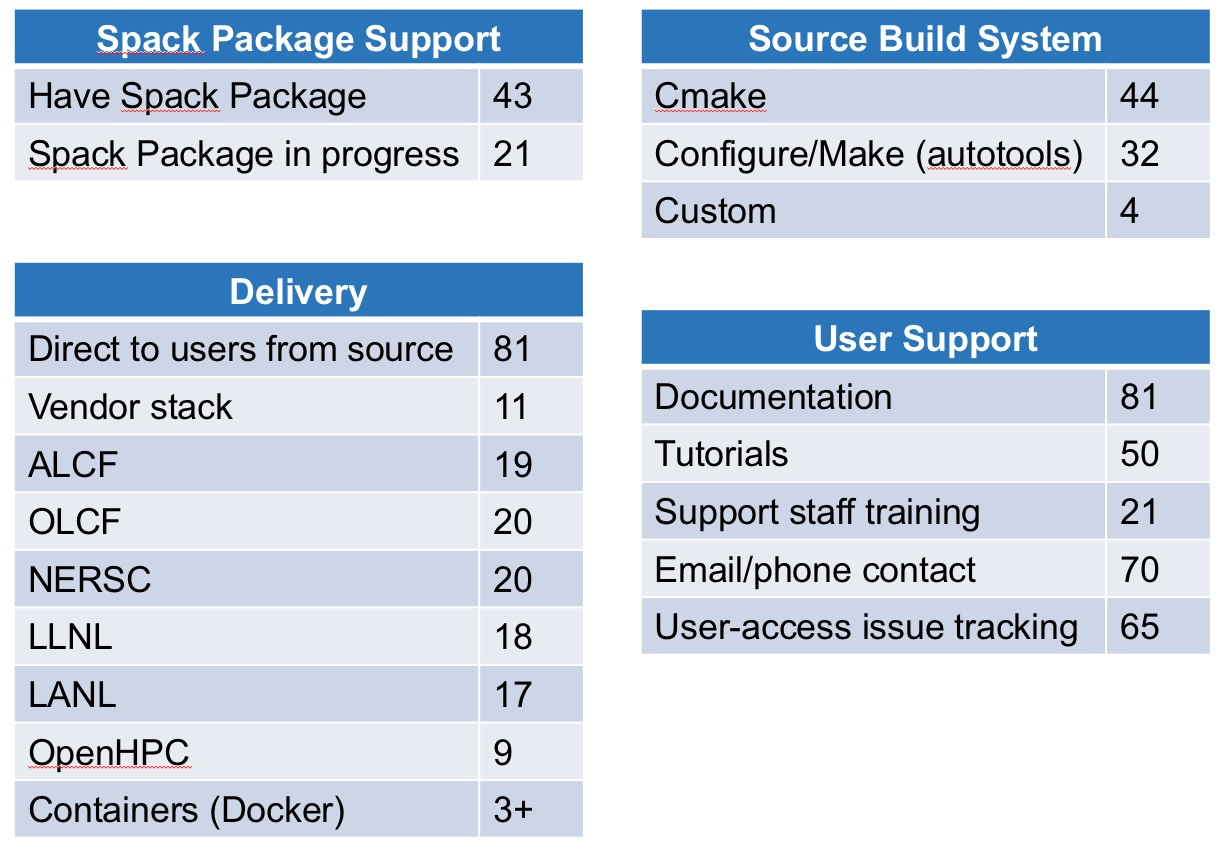
\includegraphics[width=0.7\textwidth]{ProductsOverview}

		\caption{\label{fig:productsoverview}{\small{The 33 ECP ST Projects contribute to 70 user-facing software product suites.   ECP ST products are delivered to users via many mechanisms. Provides experience we can leverage across projects.  Building via Spack is required for participating in ECP ST releases: 50 of the 70 ST product suites are available in the Extreme-scale Scientific Software Stack (E4S) V1.0, release in November 2019.}}}
	\end{center}
\end{figure}

\subsection{ECP ST Products}\label{subsect:products}
 ECP ST efforts contribute to 91 software products in five technical areas (Table~\ref{table:wbs}). 34 of the 91 products are broadly used in the HPC community and require substantial investment and transformation in preparation for Exascale architectures.  An additional 25 are important to some existing applications and typically represent new capabilities that enable new usage models for realizing the potential that Exascale platforms promise.  The remaining products are in early development phases, addressing emerging challenges and opportunities that Exascale platforms present.

\begin{table}
	\begin{tabular}{|l|l|l|}\hline
		\rowcolor{LightCyan}
		\textbf{Product} & \textbf{Website} & \textbf{Deployment Scope}\\\hline
		GASNet-EX & \url{http://gasnet.lbl.gov} & Broad\\\hline
		Kokkos & \url{https://github.com/kokkos} & Broad\\\hline
		MPICH & \url{http://www.mpich.org} & Broad\\\hline
		OpenMPI & \url{https://www.open-mpi.org} & Broad\\\hline
		RAJA & \url{https://github.com/LLNL/RAJA} & Broad\\\hline
		ROSE & \url{https://github.com/rose-compiler} & Broad\\\hline

		CHAI & \url{https://github.com/LLNL/CHAI} & Moderate\\\hline
		Global Arrays & \url{http://hpc.pnl.gov/globalarrays} & Moderate\\\hline
		Legion & \url{http://legion.stanford.edu} & Moderate\\\hline
		LLVM OpenMP compiler & \url{https://github.com/SOLLVE} & Moderate\\\hline
		OpenMP V \& V Suite & \url{https://bitbucket.org/crpl_cisc/sollve_vv/src} & Moderate \\\hline
		Qthreads & \url{https://github.com/Qthreads} & Moderate\\\hline
		Umpire & \url{https://github.com/LLNL/Umpire} & Moderate\\\hline
		UPC++ & \url{http://upcxx.lbl.gov} & Moderate\\\hline
		UMap & \url{https://github.com/LLNL/umap} & Moderate\\\hline

		BOLT & \url{https://github.com/pmodels/bolt} & Experimental\\\hline
		Argobots & \url{https://github.com/pmodels/argobots} & Experimental\\\hline
		Intel GEOPM & \url{https://geopm.github.io} & Experimental\\\hline
		PaRSEC & \url{http://icl.utk.edu/parsec} & Experimental\\\hline
		AML & \url{https://xgitlab.cels.anl.gov/argo/aml} & Experimental\\\hline
		PowerSlurm & \url{https://github.com/tpatki/power-slurm} & Experimental\\\hline
	\end{tabular}
\caption{\label{table:pmr-products} Programming Models and Runtimes Products (18 total).}
\end{table}

\begin{table}
	\begin{tabular}{|l|l|l|}\hline
		\rowcolor{LightCyan}
		\textbf{Product} & \textbf{Website} & \textbf{Deployment Scope}\\\hline

		Caliper & \url{https://github.com/llnl/caliper} & Broad\\\hline
		Dyninst Binary Tools Suite & \url{http://www.paradyn.org} & Broad\\\hline
		HPCToolkit & \url{http://hpctoolkit.org} & Broad\\\hline
		LLVM & \url{http://llvm.org/} & Broad\\\hline
		PAPI & \url{http://icl.utk.edu/exa-papi} & Broad\\\hline
		SCR & \url{https://github.com/llnl/scr} & Broad\\\hline
	    STAT & \url{https://github.com/LLNL/STAT} & Broad\\\hline
		Tau & \url{http://www.cs.uoregon.edu/research/tau} & Broad\\\hline

		mpiFileUtils & \url{https://github.com/hpc/mpifileutils} & Moderate\\\hline
		openarc & \url{https://ft.ornl.gov/research/openarc} & Moderate\\\hline
		Papyrus & \url{https://csmd.ornl.gov/project/papyrus} & Moderate\\\hline
		Program DB Toolkit (PDT) & \url{https://www.cs.uoregon.edu/research/pdt} & Moderate\\\hline
	    PRUNERS Toolset & \url{https://github.com/PRUNERS/PRUNERS-Toolset} & Moderate\\\hline
		TriBITS & \url{https://tribits.org} & Moderate\\\hline

		CHiLL Compiler & & Experimental\\\hline
		Exascale Code Gen Toolkit & & Experimental\\\hline
		Gotcha & \url{http://github.com/llnl/gotcha} & Experimental\\\hline
		Kitsune & \url{https://github.com/lanl/kitsune} & Experimental\\\hline
		QUO & \url{https://github.com/lanl/libquo} & Experimental\\\hline
		SICM & & Experimental \\\hline
		SuRF  & & Experimental\\\hline
\end{tabular}
\caption{\label{table:tools-products} Development Tools Products (21 total).}
\end{table}



\begin{table}
\begin{tabular}{|l|l|l|}\hline
		\rowcolor{LightCyan}
	\textbf{Product} & \textbf{Website} & \textbf{Deployment Scope}\\\hline
	hypre & \url{http://www.llnl.gov/casc/hypre} & Broad\\\hline
	Kokkoskernels & \url{https://github.com/kokkos/kokkos-kernels} & Broad\\\hline
	MFEM & \url{http://mfem.org/} & Broad\\\hline
	PETSc/TAO & \url{http://www.mcs.anl.gov/petsc} & Broad\\\hline
	SLATE & \url{http://icl.utk.edu/slate} & Broad\\\hline
	SUNDIALS & \url{https://computation.llnl.gov/projects/sundials} & Broad\\\hline
	SuperLU & \url{https://portal.nersc.gov/project/sparse/superlu} & Broad\\\hline
	Trilinos & \url{https://github.com/trilinos/Trilinos} & Broad\\\hline

	DTK & \url{https://github.com/ORNL-CEES/DataTransferKit} & Moderate\\\hline
	FleCSI & \url{http://www.flecsi.org} & Moderate\\\hline
	MAGMA-sparse & \url{https://bitbucket.org/icl/magma} & Moderate\\\hline
	STRUMPACK & \url{http://portal.nersc.gov/project/sparse/strumpack} & Moderate\\\hline
	xSDK & \url{https://xsdk.info} & Moderate\\\hline

	FFTX & \url{https://github.com/spiralgen/fftx} & Experimental\\\hline
	ForTrilinos & \url{https://trilinos.github.io/ForTrilinos} & Experimental\\\hline
	libEnsemble & \url{https://github.com/Libensemble/libensemble} & Experimental\\\hline
	Tasmanian & \url{http://tasmanian.ornl.gov} & Experimental\\\hline
\end{tabular}
\caption{\label{table:math-products} Mathematical Libraries Products (16 total).}
\end{table}


\begin{table}
\begin{tabular}{|l|l|l|}\hline
		\rowcolor{LightCyan}
	\textbf{Product} & \textbf{Website} & \textbf{Deployment Scope}\\\hline
	Catalyst (ALPINE) & \url{https://www.paraview.org/in-situ} & Broad\\\hline
	Darshan & \url{http://www.mcs.anl.gov/research/projects/darshan} & Broad\\\hline
	HDF5 & \url{https://www.hdfgroup.org/downloads} & Broad\\\hline
	IOSS & \url{https://github.com/gsjaardema/seacas} & Broad\\\hline
	Parallel netCDF & \url{http://cucis.ece.northwestern.edu/projects/PnetCDF} & Broad\\\hline
	ParaView (ALPINE) & \url{https://www.paraview.org} & Broad\\\hline
	ROMIO & \url{http://www.mcs.anl.gov/projects/romio} & Broad\\\hline
	VeloC & \url{https://veloc.readthedocs.io} & Broad\\\hline
	VeloC & \url{https://xgitlab.cels.anl.gov/ecp-veloc} & Broad\\\hline
	VisIt (ALPINE) & \url{https://wci.llnl.gov/simulation/computer-codes/visit} & Broad\\\hline
	VTK-m & \url{http://m.vtk.org} & Broad\\\hline
	
	ADIOS & \url{https://github.com/ornladios/ADIOS2} & Moderate\\\hline
	ASCENT (ALPINE) & \url{https://github.com/Alpine-DAV/ascent} & Moderate\\\hline
	In Situ Algorithms (ALPINE) & \url{https://github.com/Alpine-DAV/algorithms} & Moderate\\\hline
	Cinema & \url{https://github.com/cinemascience} & Moderate\\\hline
	zfp & \url{https://github.com/LLNL/zfp} & Moderate\\\hline
	
	C2C &  & Experimental\\\hline
	FAODEL & \url{https://github.com/faodel/faodel} & Experimental\\\hline
	GUFI & \url{https://github.com/mar-file-system/GUFI} & Experimental\\\hline
	HXHIM & \url{http://github.com/hpc/hxhim.git} & Experimental\\\hline
	MarFS & \url{https://github.com/mar-file-system/marfs} & Experimental\\\hline
	Mercury & \url{http://www.mcs.anl.gov/research/projects/mochi} & Experimental\\\hline
	ROVER &  & Experimental\\\hline
	Siboka &  & Experimental\\\hline
	SZ & \url{https://github.com/disheng222/SZ} & Experimental\\\hline
	TuckerMPI &  & Experimental\\\hline
	UnifyCR & \url{https://github.com/LLNL/UnifyCR} & Experimental\\\hline
\end{tabular}
\caption{\label{table:vizdata-products} Visualization and Data Products (26 total).}
\end{table}



\begin{table}
\begin{tabular}{|l|l|l|}\hline
		\rowcolor{LightCyan}
	\textbf{Product} & \textbf{Website} & \textbf{Deployment Scope}\\\hline
	Flang/LLVM & Fortran compiler \url{http://www.flang-compiler.org} & Broad\\\hline
	Spack & \url{https://github.com/spack/spack} & Broad\\\hline

	Flux &  \url{http://flux-framework.org} & Moderate\\\hline
	BEE & & Experimental\\\hline
	FSEFI & & Experimental\\\hline
	Sonar & & Experimental\\\hline
	Secure JupyterHub & & Experimental\\\hline
	Kitten Lightweight Kernel & \url{https://github.com/HobbesOSR/kitten} & Experimental \\\hline
	NRM & \url{https://xgitlab.cels.anl.gov/argo/nrm} & Experimental\\\hline
\end{tabular}
\caption{\label{table:eco-products} Software Delivery and Ecosystems Products (12 total).}
\end{table}

\subsection{Standards Committees}
An important activity for ECP ST staff is participation in standards efforts.  In many instances, our software will not be sustainable if it is not tightly connected to a standard.  At the same time, any standard has to take into account the emerging requirements that Exascale platforms need in order to achieve performance and portability.  Figure~\ref{fig:standards} summarized ECP ST staff involvement in the major standards efforts that impact ECP.

ECP ST staff are heavily involved in MPI and OpenMP standards efforts.  ECP ST staff hold several key leadership positions and have heavy involvement in all aspects. ECP ST staff also play a critical role in C++ standards efforts.  While DOE staff have only recently engaged in C++ standards, our efforts are essential to  getting HPC requirements considered, especially by contributing working code that demonstrates requirements and design. ECP ST sponsors the newest open source Fortran compiler Flang~\ref{subsubsect:flang}, a front end for LLVM.  This compiler is a rapidly emerging and essential part of the HPC ecosystem.  In particular, while ARM processors are not explicitly part of the pre-Exascale ecosystem, they are emerging as a strong contender in the future.  Flang is \textit{the} Fortran compiler for ARM-based systems.  ECP ST involvement in other committees, including the \textit{de facto} also provide valuable leverage and improved uniformity for HPC software.  Lastly, we mention the Visualization Toolkit (VTK) Architecture Review Board (ARB).  While this is only a single instance, we intend to explore the ARB model as part of our SDK efforts.
\begin{figure}[htb]
	\begin{center}
		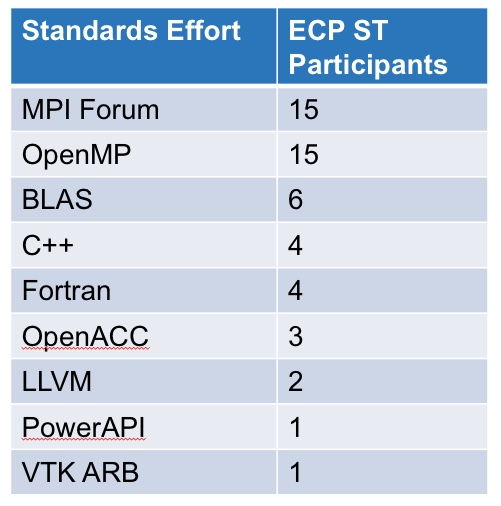
\includegraphics[width=0.5\textwidth]{StandardsInvolvement}
		
		\caption{\label{fig:standards} ECP ST staff are involved in a variety of official and \textit{de facto} standards committees.  Involvement in standards efforts is essential to assuring the sustainability of our products and to assure that emerging Exascale requirements are addressed by these standards.}
	\end{center}
\end{figure}

\subsection{Contributions to External Software Products}\label{subsection:external-contributions}
While much of ECP ST efforts and focus are on the product that we develop and support, it is important to note that some of our important work, and certainly some of our most sustainable and highly leveraged work, is done by providing requirements, analysis, design and prototype capabilities for vendor and other third party software.  Many software studies have shown that 70 to 80\% of the cost of a successful software product goes into post-delivery maintenance. Our effort summarized in Table~\ref{table:externalproducts} expressly eliminate this large cost for DOE because the product is developed and supported outside of DOE.


\begin{table}
	\begin{tabular}{|L{1.5in}|L{4in}|}\hline
			\rowcolor{LightCyan}
			Product & Contribution\\\hline
			Kokkos and RAJA & ECP efforts to provide portable on-node parallel programming and execution environments have led to new features in C++ standards \\\hline
			MPI Forum & ECP ST staff maintain several chapters of the MPI Forum, effort that require a constant involvement with the other authors, as well as participation to the online discussions related to the chapter and regular attendance of the MPI Forum face-to-face activities.\\\hline
			Flang & ECP funds development of the new open source Fortran compiler front end called Flang. Flang provides Fortran language support for LLVM backends, in a similar way as Clang provides support for C and C++.\\\hline 
			All \tools work & Starting in FY20, our \tools\ efforts are organized around delivering capabilities into the LLVM ecosystem.  \\\hline
			SWIG (www.swig.org) & The ECP ST ForTrilinos efforts contributes the capability to generate automatic Fortran bindings from C++ code.\\\hline
			TotalView debugger & ECP ST staff are engaged in co-design of OMPD, the new debugging interface for OpenMP programs, along with RogueWave engineers. This effort helps RogueWave improve their main debugging product, TotalView, by making it aware and compatible with recent advances in OpenMP debugging.\\\hline
			LLVM &  An ECP ST staff member is co-leading design discussions around the parallel IR and loop-optimization infrastructure.\\\hline
			SLATE & ECP ST math libraries efforts inform the design, implementation, and optimization of dense numerical linear algebra routines on most vendor platforms\\\hline
			Cray MPICH MPI-IO & As part of the ExaHDF5 ECP project, the ALCF worked with Cray MPI-IO developers to merge the upstream ROMIO code into the downstream proprietary Cray MPICH MPI-IO, leveraging Cray’s extensive suite of IO performance tests and further tuning the algorithm.  Cray is currently targeting its deployment in an experimental release.\\\hline
			OpenHPC & An ECP ST staff member serves on the OpenHPC Technical Steering Committee as a Component Development representative.\\\hline
		\end{tabular}
		\caption{\label{table:externalproducts} External products to which ECP ST activities contribute.  Participation in requirements, analysis, design and prototyping activities for third-party products is some of the most effective software work we can do.}
	\end{table}

%ECP ST Product Dictionary
%Note: This page is still under construction.
%
%The ECP Software Technology (ST) Product Dictionary is the official list of publicly recognized 
%names to which ECP ST efforts contribute.  While ST teams use an expanded product 
%namespace, the list on this page indicates the eventual access point for ST product development 
%efforts.
%
%This table lists only those products that are typically recognizable to users. Examples:
%1.	MPI is commonly known by users. MPICH and OpenMPI both provide implementations 
%of that product.
%2.	Fortran is a product. Flang is a particular Fortran product. LLVM is a backend for some 
%Fortran compilers.
%3.	FFT is a product. FFTX, FFT-ECP provide FFT capabilities through interchangeable 
%interfaces. 
%4.	C++ is a product. Clacc provides capabilities for Clang, as does LLVM.
%
%Product 
%Dictionary 
%List
%ST products that deliver capabilities through public products 
%(comma separated list)
%
%ADIOS
%
%AML
%
%ALPINE: Ascent, ParaView, Catalyst, Visit, LibSim, In Situ Algorithms
%
%BLAS
%
%SLATE
%
%C
%
%LLVM
%
%C++
%
%LLVM
%
%Caliper
%
%Catalyst
%
%CHAI
%
%Cinema
%
%CUDA
%
%Darshan
%
%DTK
%
%Dyninst
%
%E4S
%
%FFT
%FFTX, FFT\_ECP
%FleCSI
%
%Flux
%
%Fortran
%LLVM/Flang
%GASNet
%
%Ginkgo
%
%HDF5
%
%HPCToolkit
%
%hypre
%
%Kokkos
%
%KokkosKernels
%
%LAPACK
%
%Legion
%
%libEnsemble
%
%MarFS
%
%MFEM
%
%MPI
%MPICH, Open MPI
%OpenACC
%Clacc/LLVM
%OpenCL
%-
%OpenMP
%SOLLVE/LLVM
%PAPI
%
%Papyrus
%
%Paraview
%
%PaRSEC
%
%PETSc/TAO
%
%PnetCDF
%
%PowerStack
%
%RAJA
%
%MPI-IO
%ROMIO
%ScaLAPACK
%SLATE
%SCR
%
%SICM
%
%Spack
%
%SPOT
%
%STRUMPACK
%
%SUNDIALS
%
%SuperLU
%
%SYCL
%
%SZ
%
%TASMANIAN
%
%TAU
%
%Trilinos
%
%UMap
%
%Umpire
%
%Unify
%
%UPC++
%
%VeloC
%
%VisIt
%
%VTK-m
%
%xSDK
%
%ZFP
%
%



%%---------------------------------------------------------------------------%%
%\vspace{3in}
\clearpage
%\newpage
\section{ECP ST Project Summaries}\label{sect:project-summaries}

This section of the ECP ST Capabilities Assessment Report provides two-page summaries of each funded project.  The text provides a project overview and summarizes the key challenges, solution strategy, recent progress and next steps for the project.
\newpage
\subsection{\pmr}
This section present projects in \pmr.
\newpage

\subsubsection{\pmr\ Software Development Kits} 

\paragraph{Overview} 
The \pmr\ SDK effort is focused on identifying meaningful aggregations of products in this technical area.  SDK efforts are in the early stages of planning and execution.  Most of the work on SDKs has been driven from the \ecosystem\ technical area.  A description of the SDK effort can be found in Section~\ref{subsubsect:ecosystem-sdk}.

\newpage
\subsubsection{\stid{1.07} Exascale MPI} \label{subsubsect:mpich}
\paragraph{Overview}

MPI has been the de facto standard programming model for HPC from the
mid 90's till today, a period where supercomputing performance
increased by six orders of magnitude.  The vast majority of DOE's
parallel scientific applications running on the largest HPC systems
use MPI. These application codes represent billions of dollars of
investment. Therefore, MPI must evolve to run as efficiently as
possible on Exascale systems. Our group at Argonne developed a
high-performance, production-quality MPI implementation, called MPICH.
The focus areas of the Exascale MPI / MPICH project are: (1)
continuous improvement of the performance and capabilities of the
MPICH software to meet the demands of ECP and other broader DOE
applications, (2) coordinate vendor and supercomputing center
interactions to ensure efficient solutions to applications, and (3) be
involved in the MPI forum and standardization efforts to ensure
continuity of the work beyond this project.

MPICH team is involved in the formation of the MPI Forum and have been
deeply involved in defining the MPI standard since 1992. MPICH has
helped prototype and define the majority of the features in the MPI
standard. As such, MPICH has been one of the most influential pieces of
software in accelerating the adoption of the MPI standard by the HPC
community. MPICH has been adopted by leading vendors into their own
derivative implementations. Examples include Intel (for Intel MPI), Cray
(for Cray MPI), IBM (for IBM PE MPI), Mellanox (for MLNX-MPI), Microsoft
(for MS-MPI), and Ohio State University (for MVAPICH). MPICH and its
derivatives are exclusively used in 7 of the top 10 supercomputers in
the world today. MPICH is the recipient of a number of awards including
an R\&D 100 award.

\paragraph{Key Challenges}

While we believe MPI is a viable programming model at Exascale, both
the MPI standard and MPI implementations have to address the
challenges posed by the increased scale, performance characteristics
and evolving architectural features expected in Exascale systems, as
well as the capabilities and requirements of applications targeted at
these systems. The key challenges are:

\begin{enumerate}

\item Interoperability with intranode programming models having a high
  thread count~\cite{Hybrid1, Hybrid2, FT2} (such as OpenMP,
  OpenACC and emerging asynchronous task models);

\item Scalability and performance over complex
  architectures~\cite{Perf1, Perf2, FT2, Perf4} (including high core
  counts, processor heterogeneity and heterogeneous memory);

\item Software overheads that are exacerbated by lightweight cores and
  low-latency networks;

\item Enhanced functionality (extensions to the MPI standard) based on
  experience with applications and high-level libraries/frameworks
  targeted at Exascale; and

\item Topics that become more significant as we move to the next
  generation of HPC architectures: memory usage, power, and
  resilience.

\end{enumerate}

\paragraph{Solution Strategy}

The Exascale MPI project has the following primary technical thrusts:
(1) \textbf{Performance and Scalability} (2) \textbf{Heterogeneity}
(3) \textbf{Topology Awareness} (4) \textbf{Fault Tolerance} and (5)
\textbf{MPI+X Hybrid Programming}.

Our solution strategy started by addressing performance and
scalability aspects in MPICH related to network address
management~\cite{memscal}.  Apart from this, we also looked at
communication strategies which allow the MPI library to be as
lightweight as possible~\cite{ch41, ch42}. Other solutions include
investigation and evaluation of communication relaxation hints,
investigation of optimizations to memory scalability in MPICH and
improvements to MPI RMA operations.

Exascale MPI heterogeneity efforts~\cite{Hetero1, Hetero2, Hetero3}
started with the survey on heterogeneous memory architectures on
upcoming DOE machines and how MPICH can take advantage of
them~\cite{hexe}. The efforts also included the investigation of
utilizing heterogeneous memory inside the MPI implementation and
evaluation of applications~\cite{hetero4}. The heterogeneity efforts
further extended to investigating and developing technologies for GPU
integration for the better support of the coming Exascale
supercomputers.

Exascale MPI topology awareness efforts~\cite{Topo1,Topo2} originated
with the investigation and evaluation of hints based on topology
awareness and optimizations to virtual topology functionality in
MPICH~\cite{topo-io,topo-io2}. The other efforts include investigation
of topology-aware collectives and neighborhood collectives in
MPICH~\cite{coll} and evaluation of the selected ECP applications.

Exascale MPI fault tolerance efforts~\cite{FT1, FT2} started with
support for handling noncatastrophic errors in MPI. The second effort
included defining the scope of errors in MPI, a prerequisite for
user-level failure mitigation (ULFM). Other efforts in this direction
includes standardizing ULFM in MPI and evaluating application
suitability for fault tolerance.

Exascale MPI+X hybrid programming developed firstly with effort in
improving interoperation of MPICH with threads~\cite{interthread}.
Secondly, we developed the work-queue data transfer model for
multithreaded MPI communication~\cite{workq}. We have included support
for interaction of MPICH with user-level thread (ULT)
libraries~\cite{ULT}, primarily targeting Argobots and the BOLT
runtime~\cite{BOLT}.  Other issues that are being looked at include the
investigation and evaluation on interaction between MPI and OpenMP and
the study and evaluation of MPI endpoints.

\paragraph{Recent Progress}

Figure~\ref{fig:fy19} provides the details of major milestones completed
in FY2019. In the first milestone, we studied the performance
of the RMA improvements using the large quantum chemistry application
suite NWChem (version 6.6) with ARMCI-MPI and MPICH on the Cray XC40
supercomputer. The results shown that enabling network hardware atomics
with the info hints fully eliminated the performance bottleneck in the
Density Functional Theory (DFT) module and improved the performance
scalability of NWChem DFT. In the second milestone, we studied the
performance impact of ULFM when there is no failure. A study report has
been submitted on performance analysis of the ULFM prototype. In the
third milestone, we studied the performance of MPI Endpoints. The
results shown significant improvement of using MPI endpoints
prototype---the multithreaded MPI communication reached a message rate
that is close to the case of single-threaded MPI communication. We
concluded that exposing the application level parallelism to the MPI
through the use of endpoints enables effectively scheduling of the
traffic. In such a way, multiple hardware resource can be utilized to
reduce the contention between threads and improve performance.

\begin{figure}[htb]
  \centering
  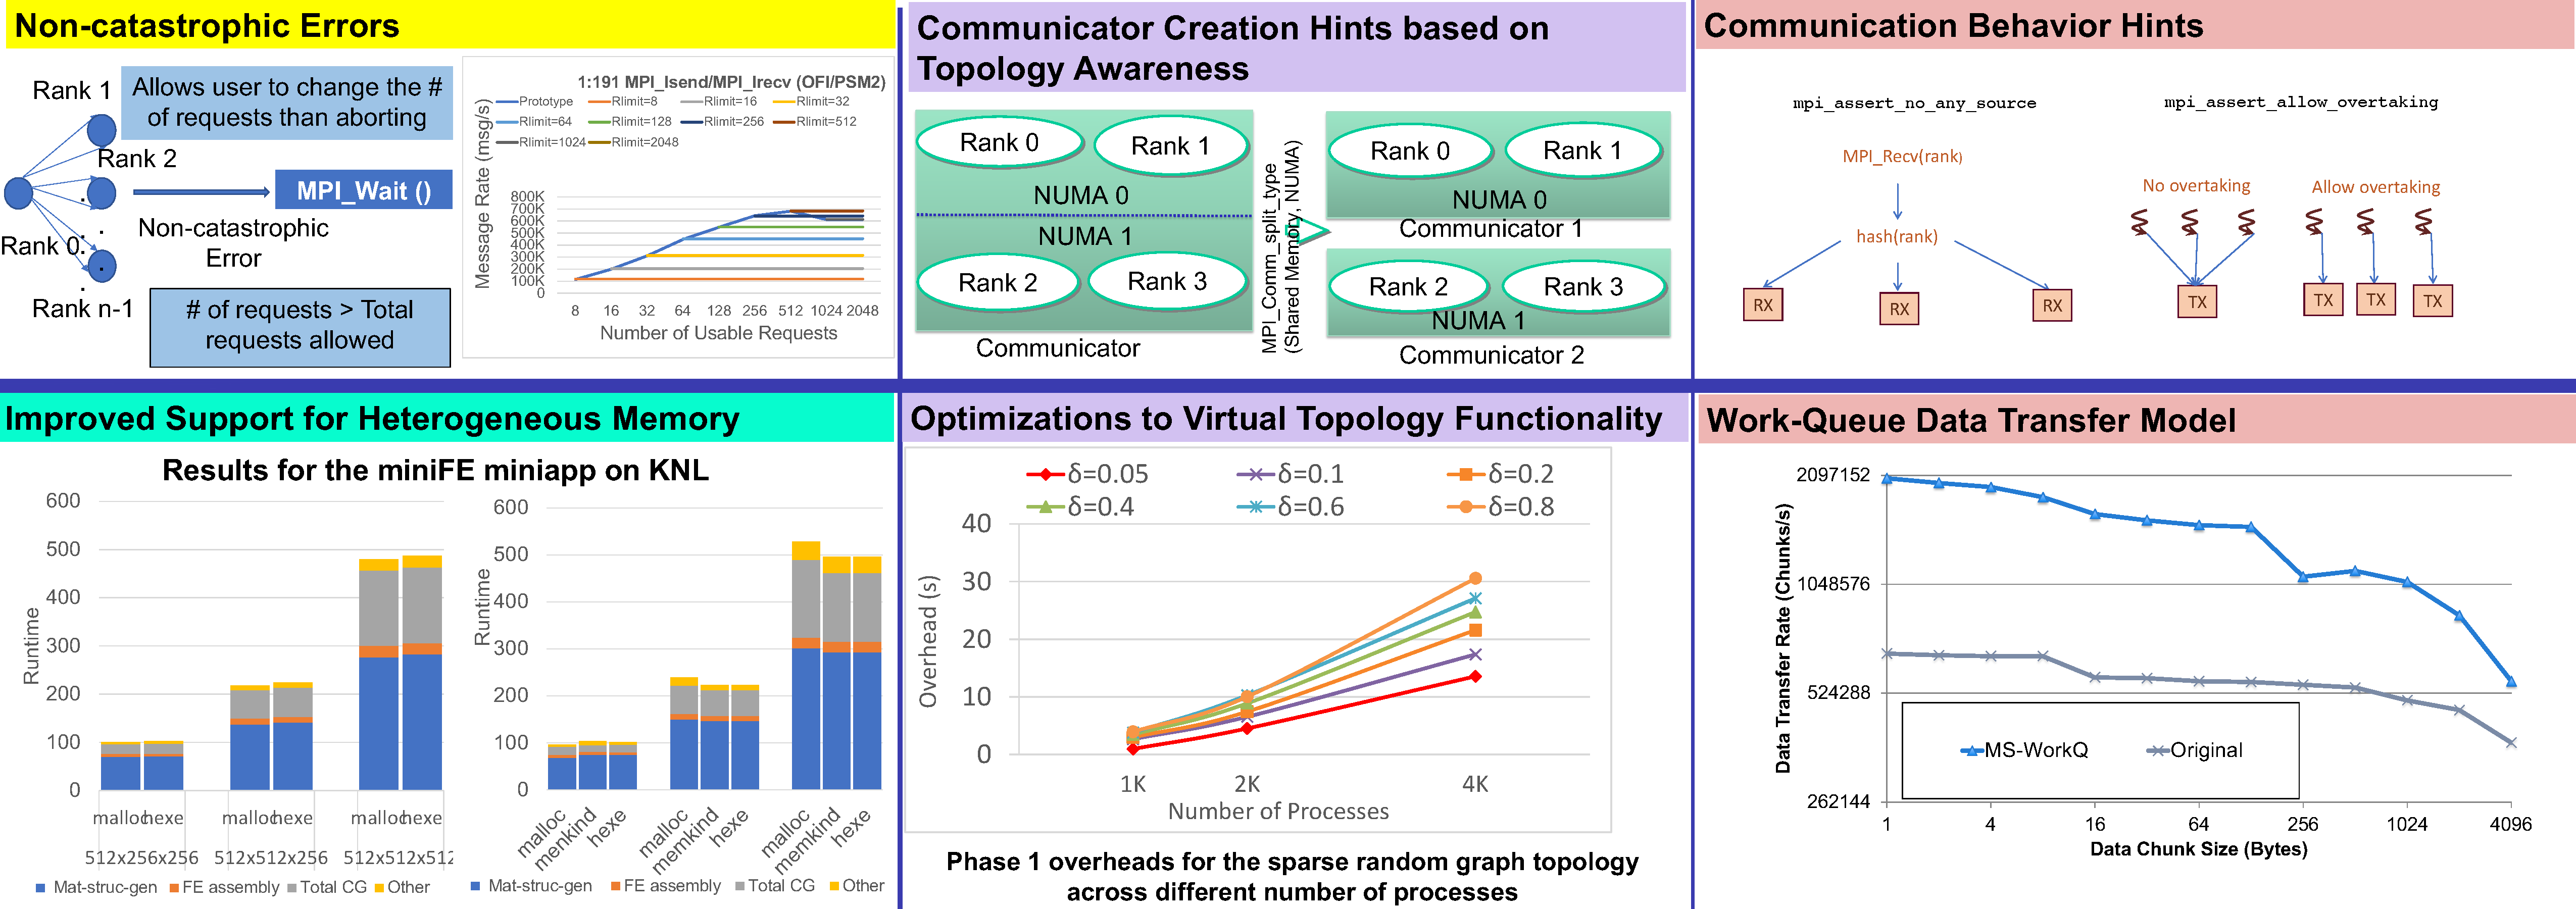
\includegraphics[width=6in]{projects/2.3.1-PMR/2.3.1.07-Exascale-MPI/MPICH-recent-milestones.pdf}
  \caption{\label{fig:fy19}Major MPICH milestones completed in fiscal year 2019}
\end{figure}

In the fourth milestone, we evaluated the benefit of using
topology-aware neighborhood collectives. We used the neighborhood
collective integration in the PETSc scalable linear solvers (KSP)
component for this evaluation. The results did show benefit, but with a
caveat that is the neighborhood collectives incurs significant setup
cost which currently overshadowing the communication benefit. The
addition of ``persistent'' collective operations in MPI-4 will allow us
to remove the per-operation setup cost. In the last milestone, we
performed comprehensive evaluation of the project which included
functional tests and performance tests.  The experiment results using
Nek5000 on OLCF Summit supercomputer shown significant improvements in
performance and scalability due to the techniques developed in this ECP
project.

\paragraph{Next Steps}
A major focus of the ongoing Exascale MPI efforts is MPI+GPU
improvements. This includes improvements for
multiple accelerator nodes and native hardware models, support for
noncontiguous data and software evaluations. Exascale MPI ongoing
efforts also includes a developing a collective selection framework for
improving the performance and scalability of collectives. We are also
making efforts in MPI standardization which includes investigation
application usage of MPI and incorporating those insights into the
MPI standard through continuous participation of the MPI standardization
process.

\newpage
\subsubsection{Legion}

\paragraph{Overview}
The Legion project focuses on the development of the Legion runtime system and programming
model. Our focus is on providing the base capabilities of an alternative task-based 
programming model that seeks to improve the amount of available parallelism and enable a 
separation of concerns of the implementation of a task from how that task and its 
associated data are mapped onto a given system architecture.  Our efforts have focused on 
addressing bugs and adding new features to the implementation but also supporting 
applications that are interested in or already using Legion. 

The Legion programming system is freely available via an open source license on the GitLab
site: \url{https://gitlab.com/StanfordLegion/legion}.

\paragraph{Key Challenges}
Legion focuses on providing a programming model and supporting implementation that will 
help address the challenges applications will face in realizing sustained performance on
what are projected to be the nature of Exascale systems. Increased scales combined with 
the challenges of programming potentially diverse accelerator and node-level processor 
technologies are responsible for a significant challenge that has yet to be fully addressed
by today's most prominent programming systems -- none of which have been fully validated 
on \emph{yet-to-be-determined} system architectures for the Exascale era of computing. 

\paragraph{Solution Strategy}
In funded collaboration between Los Alamos and Stanford University we are providing not
only the implementation of the Legion programming model but also numerous opportunities 
for application developers and participants in the ECP PathForward efforts to learn about 
Legion and data-flow and task-based approaches to programming.  We also closely work with
Combustion-Pele (AD 2.2.2.02) and the data analytics efforts in support of ExaFEL (AD 2.2.4.05)
to provide bug fixes, performance optimizations and implementation help.  We work with 
these applications and are exploring Legion with a few others, and in collaboration with 
the LANL ATDM Programming Models and Runtimes project (ST 2.3.1.02), to identify needs 
and missing features in the programming model and runtime implementation.  In addition, 
we also look at numerous aspects of having the Legion system interoperate with today's 
more widely used programming systems -- e.g. MPI and OpenMP.  This is critical in terms of
providing a path for adoption and experimentation to occur in a more productive fashion.
Finally, we are also actively exploring techniques for simplifying Legion programming to 
help assist in not only potential adoption but also in helping to educate the broader 
community about the programming model and its advantages on Exascale-class systems. 

\paragraph{Recent Progress}

Our most recent progress has been devoted to getting the S3D DNS combustion application 
running on the Summit system at OLCF and the Piz Daint system at the Swiss National 
Supercomputing Centre.  This work is utilizing the most recent version of Legion with a 
goal of both bug, scaling and overall performance enhancements.  This effort is an update
that covers new science relative to our previous work that has recently been 
published~\cite{Treichler:2017}.  At present the full set of performance and application
characteristics for this effort are still being analyzed and in particular, issues
encountered on Summit are being discussed with OLCF staff.  A early look at rough 
numbers suggest anywhere from a $26$ to over $100$X boost in performance over the 
\emph{production} (MPI-based) version of S3D.  Additional Legion features worked on in 
collaboration with LANL's ATDM efforts (ST 2.3.1.02) have resulted in much improved 
scaling capabilities due to reduced runtime overheads in comparison to past work.

Figure~\ref{fig:task-graph} on the following page, shows the task graph for a single time 
step on one node of the Legion implementation of S3D simulating an n-dodecane reaction.  
We hope to soon be able to release a more detailed analysis of the new Legion-S3D runs. 

\begin{figure}[htb]
	\centering
	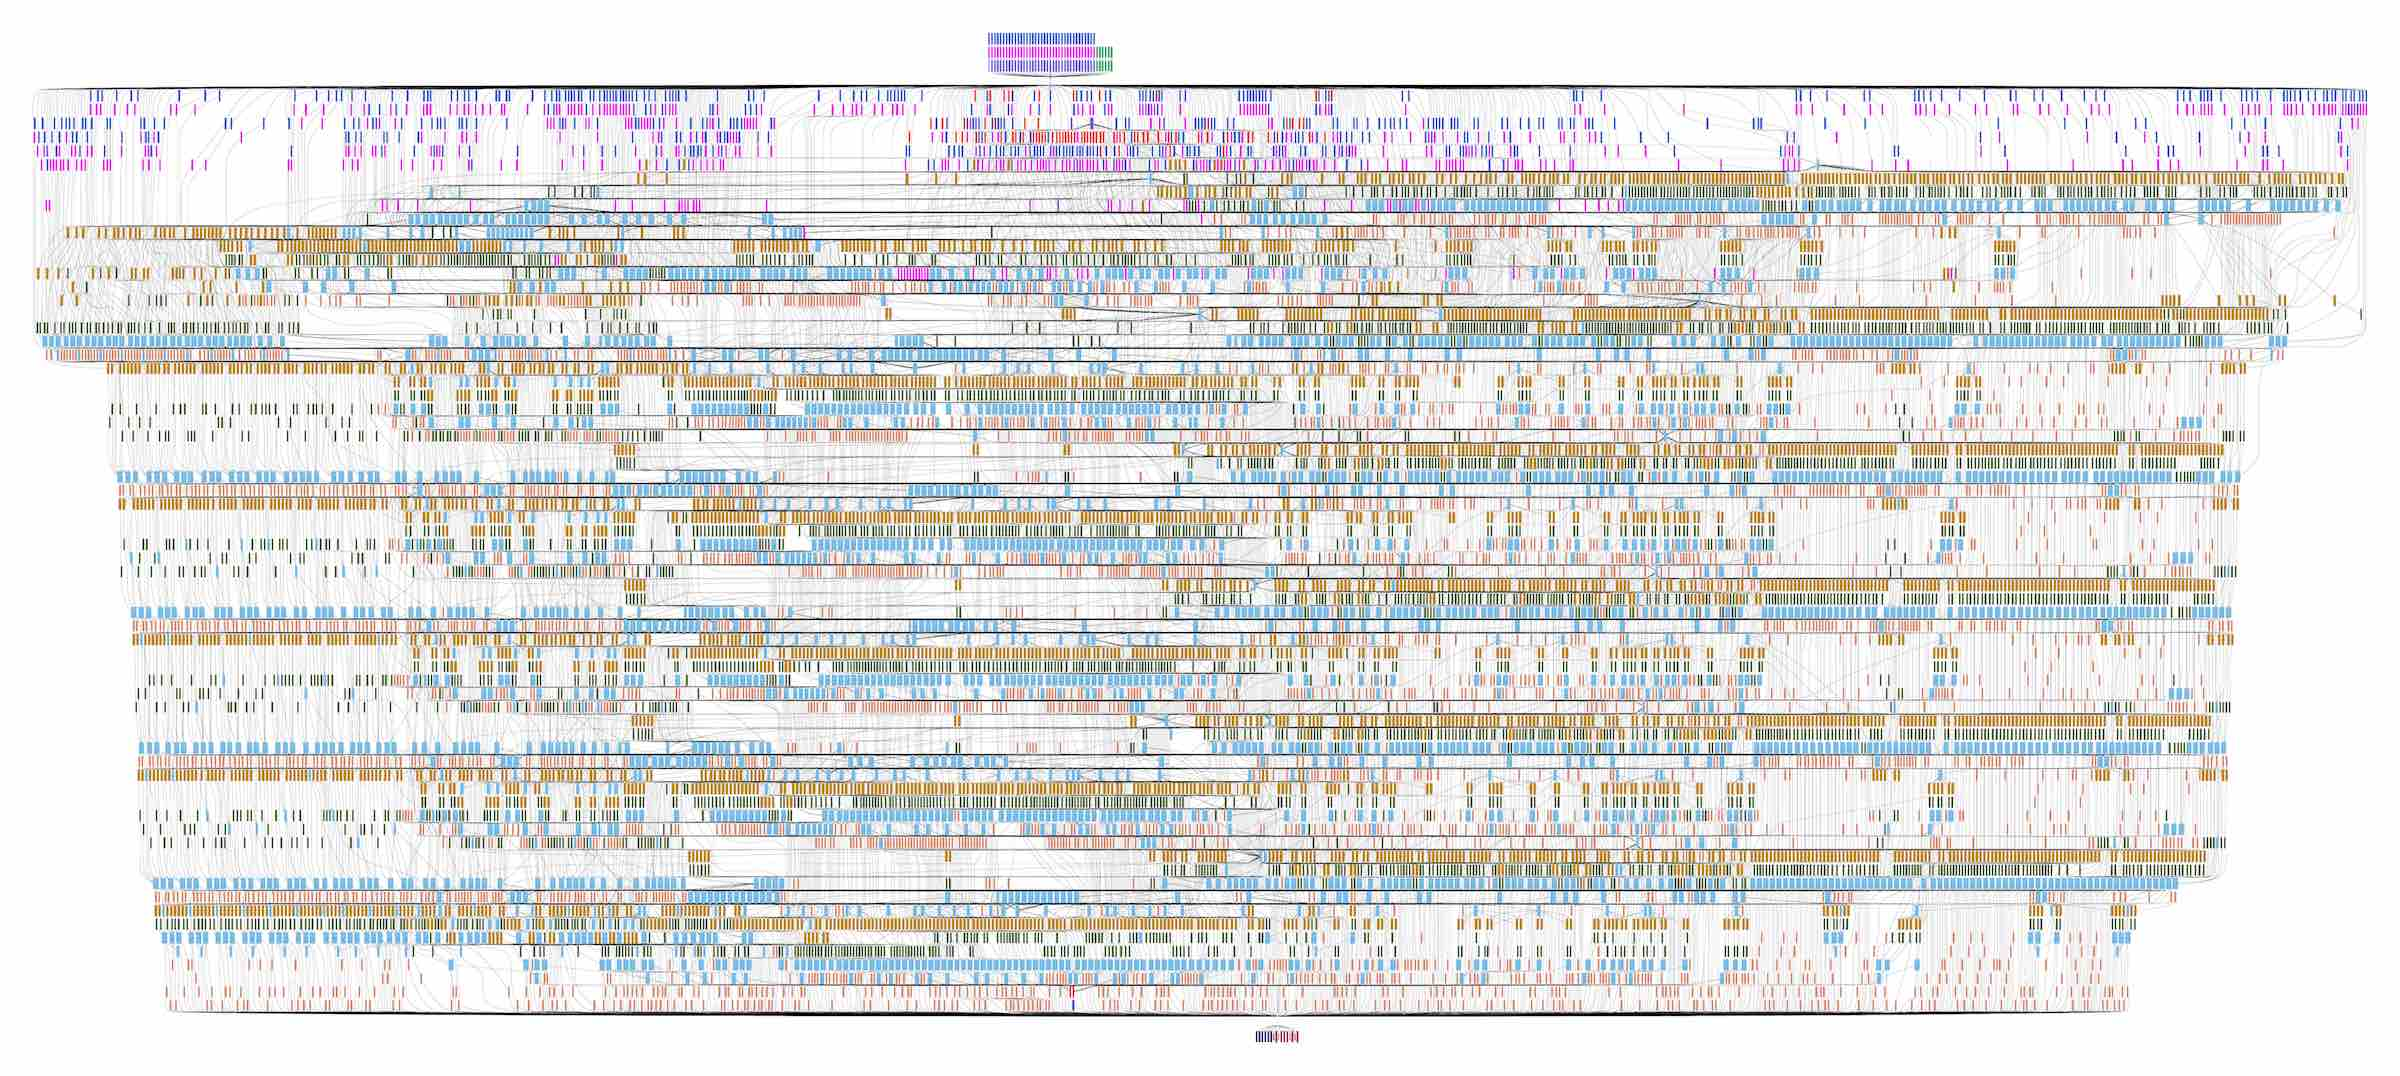
\includegraphics[width=6.5in]{projects/2.3.1-PMR/2.3.1.08-Legion/tg}
	\caption{\label{fig:task-graph}The Legion task graph for a single time step on a 
	single node.  The S3D configuration in this example is simulating n-dodecane 
	chemistry reactions in addition to the direct numerical simulation of the 
	turbulent flow.}
\end{figure}

\paragraph{Next Steps}
We will continue to focus on improving the interoperability of Legion with other programming
systems, simplifying the programming API for the Legion runtime to improve both our educational 
outreach as well as developer productivity, have regular open source releases of Legion and
also work with application teams for debugging, feature improvements and performance 
tuning.  In addition we are actively monitoring the emerging hardware technology components
that are potential targets for use in the Exascale systems that will be eventually deployed 
by both the DOE Office of Science and the NNSA. 

\newpage
\subsubsection{\stid{1.09} Distributed Tasking at Exascale: PaRSEC}


\paragraph{Overview}

The PaRSEC Environment provides a software ecosystem composed of a runtime
component to dynamically execute task-based applications on heterogeneous
distributed systems, and a productivity toolbox that comprises a development
framework for the support of multiple domain specific languages (DSLs) and
extensions, with debugging, trace collection, and analysis tools.
%
The PaRSEC project team is dedicated to solving two challenging and
interdependent problems facing the ECP developer community: First, how to create
an execution model that enables developers to express as much parallelism as
possible in their applications, so that applications effectively utilize the
massive collection of heterogeneous devices ECP machines will deploy. Second,
how to ensure the execution model is flexible and portable enough to actually
provide and sustain a performance benefit by increasing the scientific
productivity of the application developers, not only for the ECP target
environments but for the foreseeable future.

\begin{wrapfigure}[17]{l}{.45\linewidth}
  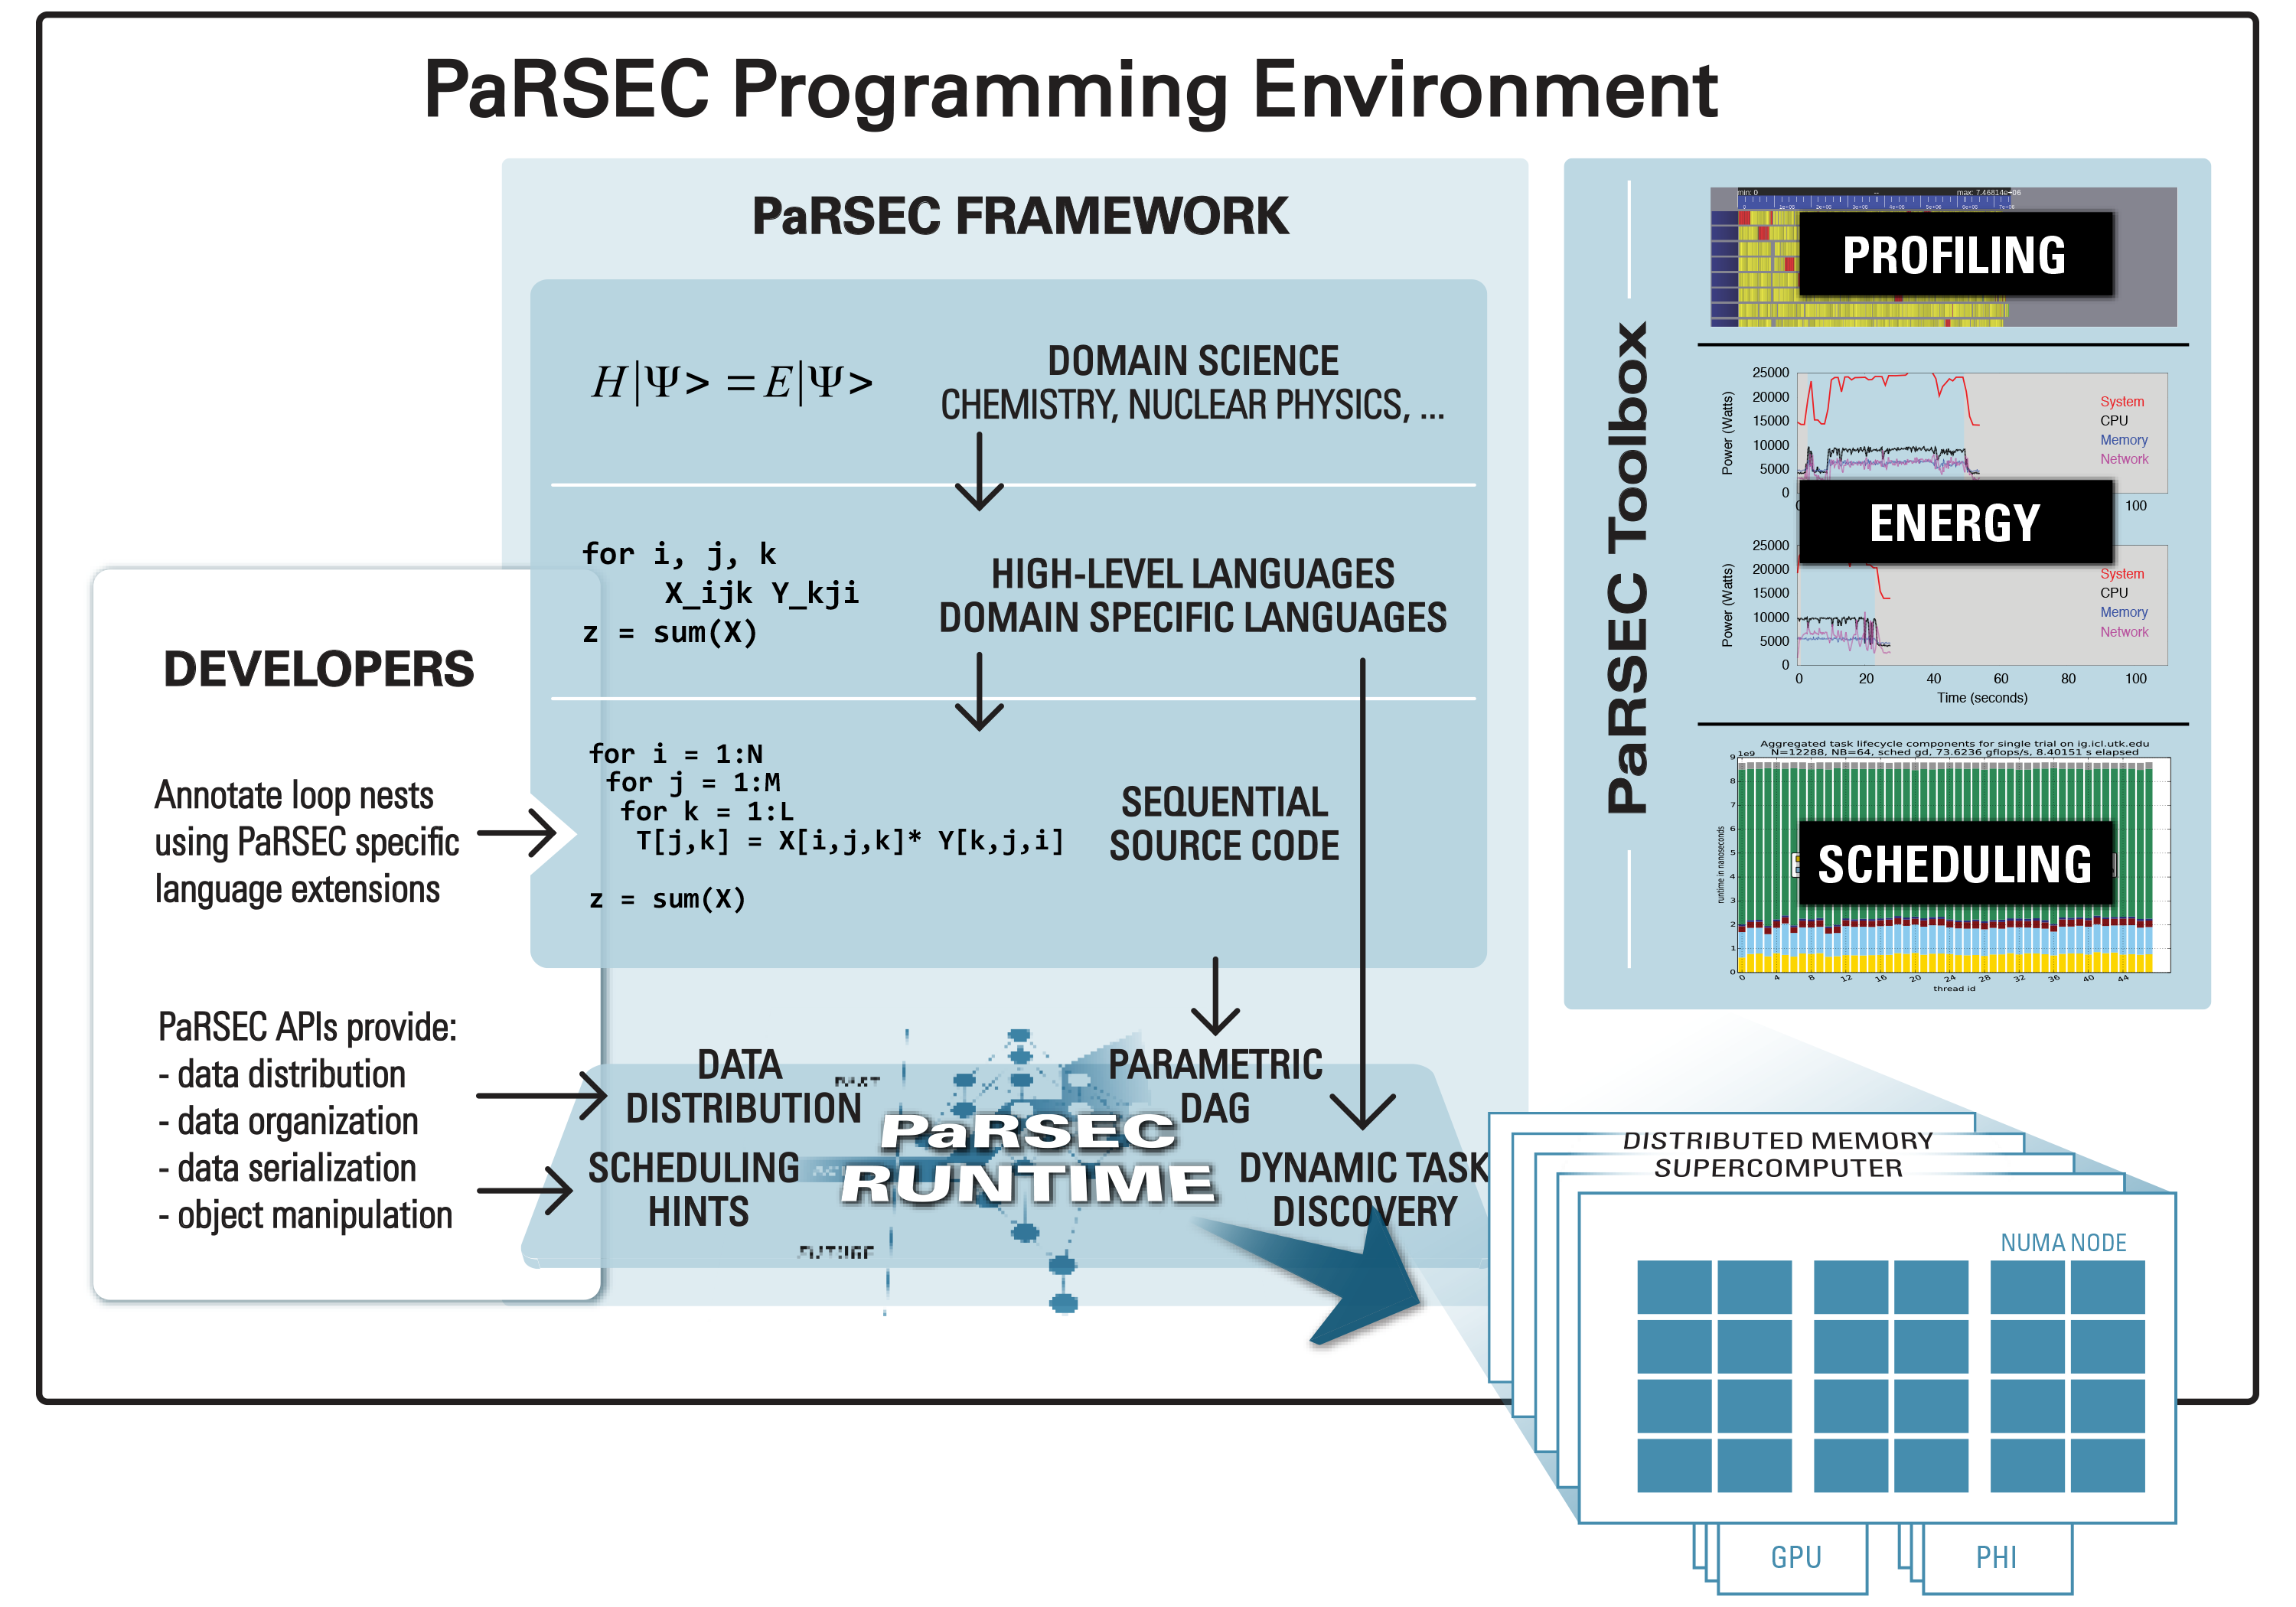
\includegraphics[scale=0.3]{projects/2.3.1-PMR/2.3.1.09-ParSEC/PaRSEC-diagram.png}
  \caption{PaRSEC architecture\label{fig:parsec} based on a modular framework where each
           component can be dynamically activated as needed.}
\end{wrapfigure}
%
PaRSEC is an open source, community-based implementation of a generic task-based
runtime that is freely available, and used by an increasing number of software
libraries.
%  The PARSEC development team is mainly comprised of research staff at % UTK,
%  but regular contributions from the community are provided via our presence %
%  on GitHub and Bitbucket.
The project focuses on providing a stable and efficient infrastructure for quick
prototyping of different approaches to define task-based languages able to
exploit the full range of capabilities of Exascale platforms. Without such a
project, and based on the current state of task-based runtimes, potential users
will be stuck either in fixed programming paradigms, or with a particular,
potentially less efficient, mix of programming languages. The DTE project
provides means to maintain a high competitiveness in the field leading to more
innovation on addressing the challenges we are facing toward scalable,
performant and Exascale ready programming paradigms.

\paragraph{Key Challenges}
%\textit{Describe what is hard to do, why it is challenging.}

As Exascale platforms delivery become a closer deadline, a increasing number of
aspects of the hardware and software environment still pose challenges. First
and foremost, keeping pace with the architectural changes on current and future
platforms requires changes not only on how we take advantage of the hardware
capabilities, but how we reshape our algorithms and applications to expose
enough parallelism to maximize the use of the underlying hardware. The number of
nodes, threads per node, memory hierarchies and support for increased
computational capabilities (accelerators) will continue to increase, while the
currently available programming paradigms are still struggling with parallelism
at the node level.

\paragraph{Solution Strategy}
%\textit{Describe your basic strategy for addressing the challenges.}
The approach followed in PaRSEC is to provide a low-level, flexible and dynamic
runtime able not only to schedule tasks at the node level, but to handle data
transfers between different memory (both inter and intra nodes), memory
hierarchies, heterogeneous architectures with support for accelerators with a
simple programming scheme. The proposed approach envisions a middle-ground
solution, addressing both hardware and software challenges. At the hardware
level a team of dedicated developers extends PaRSEC to map it's capabilities to
the hardware and to improve it's scalability and performance. At the upper
software level the runtime interactions are through Domain Specific Languages
with the target domain scientists in mind, that will facilitate the expression
of algorithmic parallelism with familiar constructs mapped on the exposed
low-level capabilities. To facilitate the integration of PaRSEC-driven libraries
into larger and complex applications, PaRSEC natively interoperate with other
programming paradigms, including some target of the ECP PMR support, such as
PGAS, MPI, OpenMP and Kokkos. This integration provides a smooth transition for
library developers that embrace the PaRSEC runtime, providing a platform where a
shift to a new programming paradigms can be done in stages of increased
complexity~\cite{lorapo-protools,BLR_LU,parsec_pdgemm}.
% In this model, PaRSEC remains in full control of data tracking and
% allocation on the managed accelerator.

\paragraph{Recent Progress}

The software release (2019.11) provides many new additions to the low-level task
runtime, supports for a number of hardware capabilities (GPU, NVLink, P9 atomic
ops), brings significant improvements to the performance and scalability of the
runtime, and addresses many pending issues.
%
% The installation system has been improved to take advantage of the latest
% capability of CMake, and scripts for seamless integration in the ECP software
% ecosystem (via SPack). Significant improvements have also been added on the
% performance and scalability of the runtime, as shown by the results below.
%
On the software quality side, the PaRSEC runtime has been evaluated and amended
to compile and run on all pre-Exascale platforms (ALCF Mira, Theta; OLCF
Summit). PaRSEC now includes a Spack definition file to ease the deployment on
future target systems as part of the system software SDK effort.

\begin{wrapfigure}{l}{.45\linewidth}
\centering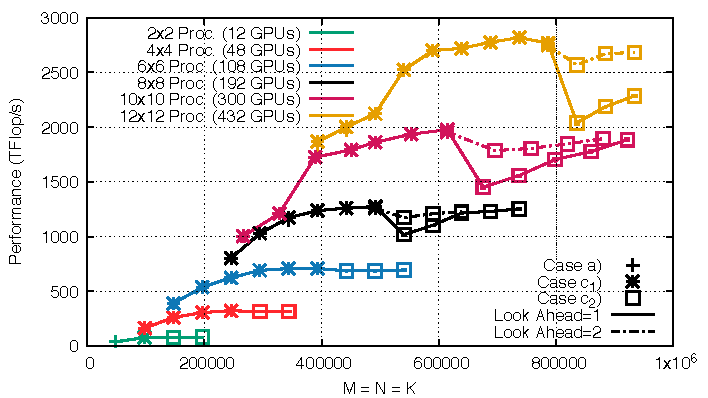
\includegraphics[scale=0.55]{projects/2.3.1-PMR/2.3.1.09-ParSEC/gemm_summit_mean.pdf}
\caption{Strong-scaling performance of the matrix-matrix multiplication
(PDGEMM)\label{fig:PDGEMM}} \end{wrapfigure} The DTE GPU support engine has been
refactored, addressing some of the existing limitations in data management
(allocation and transfer), and adding support for NVLink capabilities to
minimize the transfer cost between GPUs on the same node. All these improvements
have enabled unprecedented performance on distributed, multi-GPU platforms for
real applications.
%
Figure~\ref{fig:PDGEMM} shows a strong scaling performance of PDGEMM from our
DPLASMA math library using PaRSEC to power one of the most compute intensive
operation and study the implementation scalability with an increasing problem
and number of computing elements size. This integration illustrates the runtime
capability to obtain high efficiency for such operation independent on the
number of resources involved in the computation, even in scenarios where the
memory required for the storage of the matrices is larger than the total amount
of memory available on the GPU. A pro-active data transfer management system and
an efficient data transfer mechanisms are some of the PaRSEC underlying features
that enable such level of performance.

An important aspect of the DTE project is to define and prototype scalable
domain specific languages that enable a productive expression of parallelism for
end-user communities. PaRSEC presents multiple programming interfaces
(Parameterized Task Graphs for maximum parallelism, the popular serial task
insertion dataflow model to provide direct access to the runtime). In addition
the DTE team is in close contact with application teams to define parallel
abstractions that are suitable for their domain usage. Notably, the PaRSEC team
has ongoing collaboration with the SLATE linear algebra package and NWChemEx and
GAMESS chemistry package teams. The PaRSEC development team did the first step
toward the integration of their framework into the SLATE (2.3.3.09) in the
context of the shared milestone (STPM11-23). The first prototype of the
application ran in a distributed environment and showed the capability of the
SLATE library using a modern fully capable runtime system. This work involved
enhancing the insert task interface available in the ParSEC runtime to map onto
the logic of a SLATE algorithm.

\begin{wrapfigure}[16]{l}{.45\linewidth}
\vspace*{-1em}\centering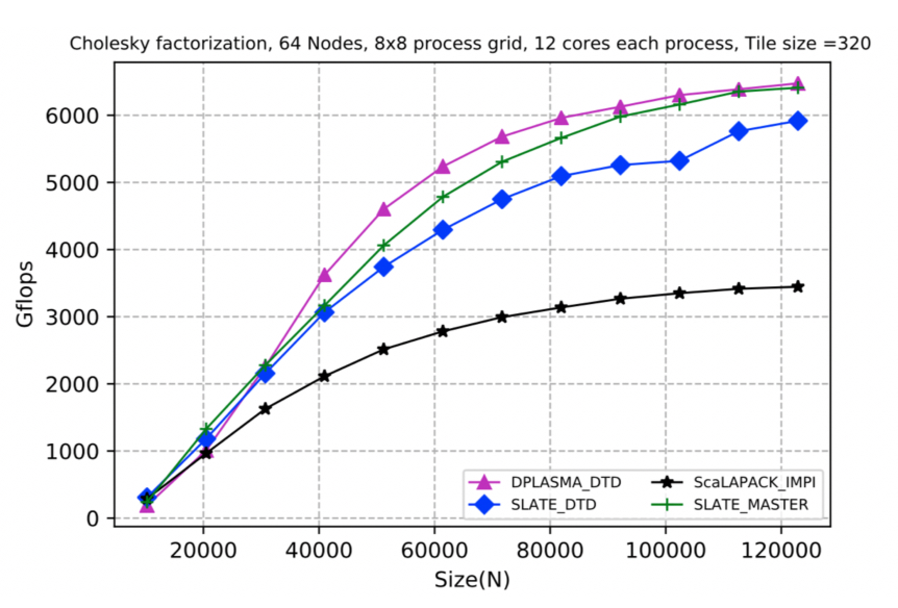
\includegraphics[scale=0.50]{projects/2.3.1-PMR/2.3.1.09-ParSEC/slate_updated_nacl.pdf}
  \caption{Comparison of DPLASMA and SLATE Cholesky factorization over PaRSEC with
           SLATE and ScaLAPACK on 64 nodes 12 cores each\label{fig:slate-parsec}}
\end{wrapfigure}
%
In figure~\ref{fig:slate-parsec}, we compare the integration of SLATE
and PaRSEC against the state of the art. First against the two legacy
domain specific languages that have the capability to do linear
algebra; then against the regular SLATE using OpenMP for intra-node
parallelism, and MPI for communication; and finally against ScaLAPACK,
which is the reference for distributed linear algebra.


\paragraph{Next Steps}
%\textit{Describe what you are working on next.}
% Improve DTE accelerator support and interoperability with other
% programming models
To provide programmers with more supervision over how accelerators are
integrated and used by the runtime, a need to provide finer control of the
resource usage by the runtime system has arisen. We are developing new APIs to
allow the programmers to advise the runtime system with respect to data
placement, prefetching, and management of cache.
%
Programming interoperability should not be limited to node-level programming
models but should extend to distributed programming. Execution modes where part
of the application is expressed in native MPI (including communicating tasks)
and other parts using PaRSEC DSLs, running above the task system in a tightly
coupled manner, are being developed.

% Facilitate DSL integration

% Provide better libraries and tools integration
The set of tools that come with the PaRSEC runtime environment to
assess performance, find bottlenecks, improve scheduling and debug the
task-based application are being improved to expose the information
in a format compatible with TAU, Score-P and other
tools that are already familiar to ECP users.

\newpage
\subsubsection{\stid{1.14} GASNet-EX}
\paragraph{Overview} 

The Lightweight Communication and Global Address Space Support project (Pagoda)
is developing GASNet-EX~\cite{gasnet-site}, a portable high-performance communication layer
supporting multiple implementations of the Partitioned Global Address Space
(PGAS) model.
GASNet-EX clients include Pagoda's PGAS programming interface UPC++~\cite{Bachan:paw17,upcxx-site}
 and the Legion Programming
System~\cite{bauer2012legion,legion-site} (WBS~2.3.1.08).

GASNet-EX's low-overhead communication mechanisms are designed to maximize
injection rate and network utilization, tolerate latency through
overlap, streamline unpredictable communication events, minimize
synchronization, and efficiently support small- to medium-sized
messages arising in ECP applications.  GASNet-EX enables the ECP
software stack to exploit the best-available communication mechanisms,
including novel features still under development by vendors.  The
GASNet-EX communications library and the PGAS models built upon it
offer a complementary, yet interoperable, approach to MPI with OpenMP,
enabling developers to focus their effort on optimizing
performance-critical communication.

We are co-designing GASNet-EX with the UPC++ development team with
additional input from the Legion and
(non-ECP) Cray Chapel~\cite{chapel-chapter,chapel-site} projects.

\paragraph{Key  Challenges}

Exascale systems will deliver exponential growth in on-chip parallelism and
reduced memory capacity per core, 
increasing the importance of strong
scaling and finer-grained communication events.  
Success at Exascale demands that
software needs to minimize the work performed by lightweight cores and avoid the
overhead of long, branchy serial code paths; 
this motivates a requirement for efficient
fine-grained communication.
These problems are exacerbated by application trends; many of the ECP applications require
adaptive meshes, sparse matrices,
or dynamic load balancing.
All of these characteristics favor the use of
low-overhead communication mechanisms that
can maximize injection rate and network utilization, tolerate latency through
overlap, accommodate unpredictable communication events, minimize synchronization,
and efficiently support small- to medium-sized messages. The ECP software stack
needs to expose the best-available communication mechanisms, including novel
features being developed by the vendor community.

\paragraph{Solution Strategy}

The PGAS model is a powerful means of addressing these
challenges and is critical in building other ECP programming systems,
libraries, and applications.  We use the term {\em PGAS} for models that support
one-sided communication, 
including contiguous and non-contiguous remote memory access (RMA) operations such as put/get
and atomic updates. Some of these models also include support for remote function invocation.
GASNet-EX~\cite{gasnet-lcpc18} is a communications library that provides the foundation for implementing
PGAS models, and is the successor to the widely-deployed GASNet library.
We are building on over 15 years of experience with the GASNet~\cite{gasnet-spec,gasnet-site}
communication layer to provide production-quality implementations that include
improvements motivated by
technology trends and application experience.  

The goal of the GASNet-EX work is to provide a portable, high-performance GAS
communication layer for Exascale and pre-Exascale systems, addressing the challenges
identified above.
GASNet-EX provides interfaces that efficiently match the RDMA capabilities of modern
inter-node network hardware and intra-node communication between distinct address spaces.
New interfaces for atomics and collectives have enabled offload to current
and future network hardware with corresponding capabilities.
These design choices and their implementations supply the low-overhead communications
mechanisms required to address the requirements of Exascale applications.

\begin{figure}[htb]
  \centering
  \subfloat[8-byte RMA Latencies\label{fig:rma-lat-bars}]{
     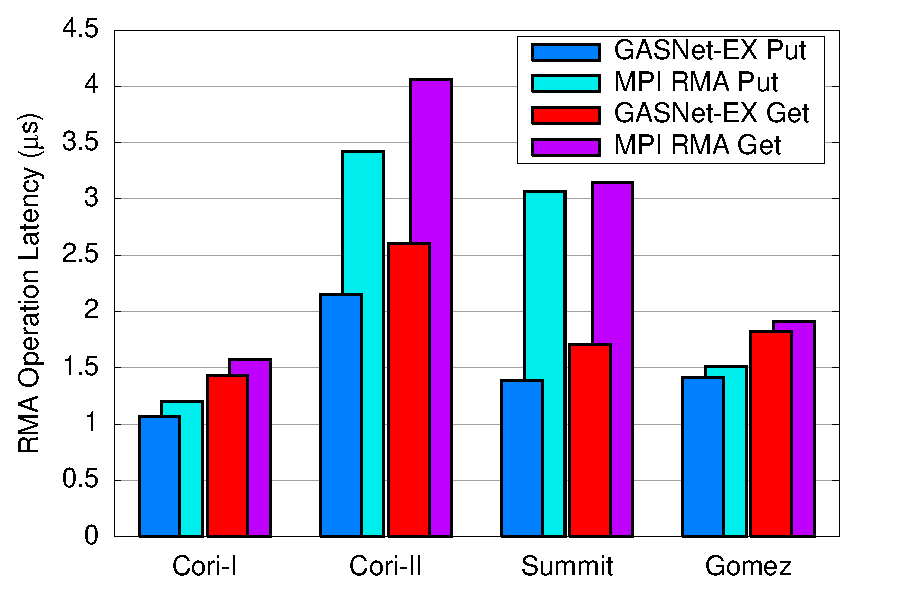
\includegraphics[width=0.432\textwidth]{projects/2.3.1-PMR/2.3.1.14-UPCxx-GASNet/latency_bars.pdf}
  }
  \subfloat[Summit Flood Bandwidth\label{fig:summit-bw}]{
     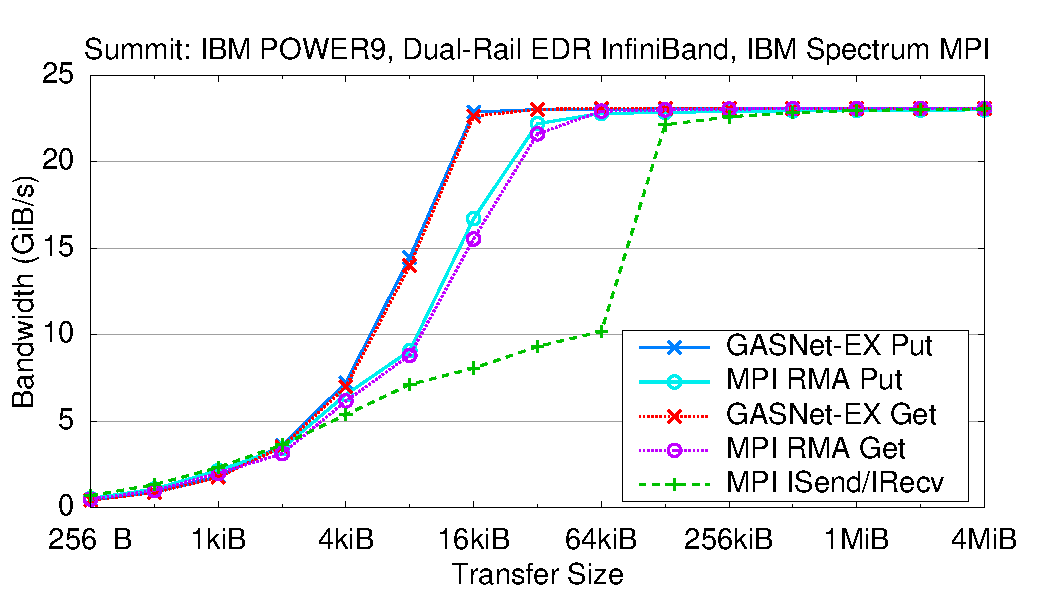
\includegraphics[width=0.504\textwidth]{projects/2.3.1-PMR/2.3.1.14-UPCxx-GASNet/Summit-slide-BW.pdf}
  }
  \caption{\label{fig:gasnet-ex-rma} Selected GASNet-EX vs. MPI RMA Performance Results}
\end{figure}

Figure~\ref{fig:gasnet-ex-rma} shows representative results from a
paper~\cite{gasnet-lcpc18} comparing
the RMA performance of GASNet-EX with MPI on multiple systems including
NERSC's Cori and OLCF's Summit%
\footnote{The paper's results from Summitdev
have been replaced by more recent (June 2019) results from OLCF's newer Summit system.}.
These results demonstrate the ability of a PGAS-centric runtime to
deliver performance as good as MPI, and often better.
%
The paper presents experimental methodology and system descriptions, which are
also available online~\cite{gasnet-site}, along with results for additional
systems.

Figure~\ref{fig:rma-lat-bars} shows the latency of 8-byte RMA Put and Get operations on
four systems, including two distinct networks and three distinct MPI
implementations.
%
GASNet-EX's latency is 6\% to 55\% better than MPI's on Put and 5\% to 45\%
better on Get.
%
Algorithms sensitive to small-transfer latency may become practical in PGAS
programming models due to these improvements relative to MPI.

Figure~\ref{fig:summit-bw} shows flood bandwidth of RMA Put and Get over the
dual-rail InfiniBand network of OLCF's Summit.
GASNet-EX's bandwidth is seen to rise to saturation at smaller
transfer sizes than IBM Spectrum MPI, with the most pronounced differences
appearing between 4KiB and 32KiB.
%
Comparison to the bandwidth of MPI message-passing (dashed green series) illustrates the
benefits of one-sided communication, a major feature of PGAS models.


\paragraph{Recent Progress}

Work on GASNet-EX in the past year has covered several distinct areas.

Co-design work is on-going with the UPC++, Legion and Chapel developers.  These
interactions are bi-directional, guiding design and implementation decisions
made in GASNet-EX as well as in the client runtimes.
%
Recent work~\cite{gasnet-reassembly} for the Cray Aries network has yielded
significant performance improvement on systems of importance to UPC++ and Legion.
Specifically, implementation of a new target-side reassembly protocol improved
AM Long end-to-end latency by up to 33\%, and the effective bandwidth by up to
49\%, while also enabling asynchronous source completion that drastically reduces
injection overheads.

We have begun work to improve interoperability of GASNet-EX and MPI within the
same executable.  Together with the Exascale MPI project (WBS~2.3.1.07) we have
developed an initial implementation of a small library to manage cooperative
progress of multiple communications runtimes.  We have demonstrated the ability
of this library, with suitable calls added to GASNet-EX and MPICH, to resolve
two canonical examples of the class of deadlock it is meant to prevent.

We have completed work to leverage features of the InfiniBand network
present in OLCF's Summit.  One such development is modifications to fully
utilize the multiple InfiniBand network ports (a.k.a ``rails'') in a Summit
node.  Another is use of Mellanox's ``ODP'' (On-Demand Paging) to provide
efficient and robust RDMA transfers to and from memory in a processes' stack
and dynamic heap.

\paragraph{Next Steps}

Our next efforts include:
\begin{enumerate}

\item \textbf{Device (GPU) Memory Support}.
GASNet-EX's RMA APIs have been designed to enable hardware offload of
transfers to and from GPU memories (\textit{e.g.} use of GPUDirect).
Near-future work includes implementation of this capability for OLCF's
Summit.  This work includes adding support for multiple
communications endpoints and multiple memory segments, which also provide
benefit to multi-threaded runtimes by reducing contention for shared resources.

\item \textbf{Specialization for InfiniBand}.  Network-specific implementations
of new GASNet-EX features for the InfiniBand network will provide performance
benefits on systems such as OLCF's Summit.  The benefits of such specialization
for the Cray Aries network has been demonstrated previously~\cite{gasnet-aries}.

\item \textbf{Client-Driven Tuning}.  In collaboration with authors of client
runtimes using GASNet-EX (most notably UPC++ and Legion) and their users (such
as ExaBiome), we will continue to identify and address any significant
bottlenecks or performance anomalies which are discovered.

\end{enumerate}

\subsubsection{UPC++} 
\paragraph{Overview} 
The UPC++ project is developing a C++ library
that supports Partitioned Global Address Space (PGAS) programming~\cite{Bachan:paw17}.
The UPC++ project began in 2012 with a prototype designated V0.1, described in \cite{zheng:ipdps14}.
We are revising the library under the auspices of the DOE's Exascale Computing
Project, to meet the needs of applications requiring PGAS support.
UPC++ is well-suited for implementing elaborate distributed data structures where
communication is irregular or fine-grained. The UPC++ interfaces for
moving non-contiguous data and sending Remote Procedure Calls (RPC)
are composable and closely resemble those used in modern C++.

UPC++ is needed for ECP because it delivers low-overhead communication that runs
at close to hardware speeds, embracing 
interest by vendors in the PGAS model because it 
efficiently matches the RDMA mechanisms offered by
network hardware and on-chip communication between distinct address
spaces.  
Because ECP applications rely on irregular representations
to improve accuracy and conserve memory, the UPC++ library provides
an essential ingredient for the ECP software stack.  It will enable
effective scaling in Exascale software by minimizing the work funneled
to lightweight cores, avoiding the overhead of long, branchy serial
code paths, and supporting efficient fine-grained communication.  The
importance of these properties is exacerbated by application trends;
many ECP applications require the use of adaptive meshes, sparse
matrices, dynamic load balancing, or similar techniques.  UPC++'s
low-overhead communication mechanisms can maximize injection rate and
network utilization, tolerate latency through overlap, streamline
unpredictable communication events, minimize synchronization, and
efficiently support small- to medium-sized messages arising in such
applications.  UPC++ will enable the ECP software stack to exploit
the best-available communication mechanisms, including novel features
being developed by vendors.  This library offers a complementary,
yet interoperable, approach to MPI with OpenMP, enabling developers to
focus their effort on optimizing performance-critical communication.

\paragraph{Key  Challenges}

As the result of technological trends, the cost of data motion is steadily increasing relative to that of computation.  To reduce communication costs we need to 
either reduce the software overheads or hide  communication behind available computation. UPC++ addresses both strategies.
To reduce software overheads, UPC++ takes advantage of the GASNet-EX communication library's \cite{gasnet-spec}
low-overhead communication as well as access to any special hardware
(see the accompanying report on GASNet-EX, which is being co-designed).
UPC++ supports asynchronous communication via classic one-sided communication
(i.e. puts and gets) and remote procedure calls, to support communication hiding.


% A challenge in the ECP-ST effort is to maintain interoperability among run times,
% that invoke the back end to carry out communication. The difficulty is that each
% backend operates under the assumption that it "owns" the network.
% But many ECP applications employ (or will under ECP) multiple runtimes;
% thus interoperability is of paramount concern.
% Our approach is conservative; so long as entries and exits between different
% models is sufficiently coarse grained, then it is feasible to synchronize
% at a barrier at each transition.

\paragraph{Solution Strategy}

The UPC++ project has two primary thrusts:
\begin{enumerate}
\item \textbf{Increased performance through reduced communication costs:} The
UPC++ programmer can expect communication to run at close to hardware speeds.
Asynchronous execution enables an application to hide communication behind
available computation.

\item \textbf{Improved productivity:}  UPC++'s treatment of asynchronous
execution relies on futures and promises, and these simplify the management of
asynchrony.

\end{enumerate}

The PGAS one-sided communication employed by UPC++ (get/put)
benefits application  performance by mapping tightly onto the RDMA
communication supported by the communication network. GASNet-EX provides the
thin middleware
needed to enable this model to run at close to hardware speeds, across platforms ranging from laptops to supercomputers.
One-sided communication also has another benefit.
It decouples synchronization from data motion,
avoiding synchronization overheads of two-sided communication (e.g. message passing).

UPC++'s Remote Procedure Call, which is built on GASNet Active Messages,
provides additional control over asynchronous execution, by enabling
the programmer
to execute procedure calls on remote processors.
RPC is useful in managing access to complicated irregular data structures,
and in expressing asynchronous task execution.

UPC++ addresses productivity via one-sided data motion, remote procedure calls,
and via the provision of futures.
Futures enable the programmer
to capture data readiness state, which is useful in making scheduling decisions, 
via continuations, to execute asynchronously as dependencies become
satisfied. Chaining and conjoining
of asynchronous operations simplify treatment of their completion.



\paragraph{Recent Progress}

symPACK is a direct linear solver for symmetric positive definite sparse matrices.
Originally written using the legacy UPC++ V0.1, we have recently ported symPACK to
use the latest release of UPC++ V1.0. Our experiments conducted on NERSC Edison
confirm that the new UPC++ version preserves the performance of the symPACK solver.


\begin{figure}[htb]
%  \captionsetup{format=centering}
	\centering
	%\includegraphics[width=6in]{sympack-perf}
  \subfloat[\textbf{Push} -- MPI two-sided communication\newline\textbf{Pull} -- UPC++: RPC + RMA Get when ready\newline 2 variants with and without event driven scheduling]{
    \label{fig:sympack:comm}
	  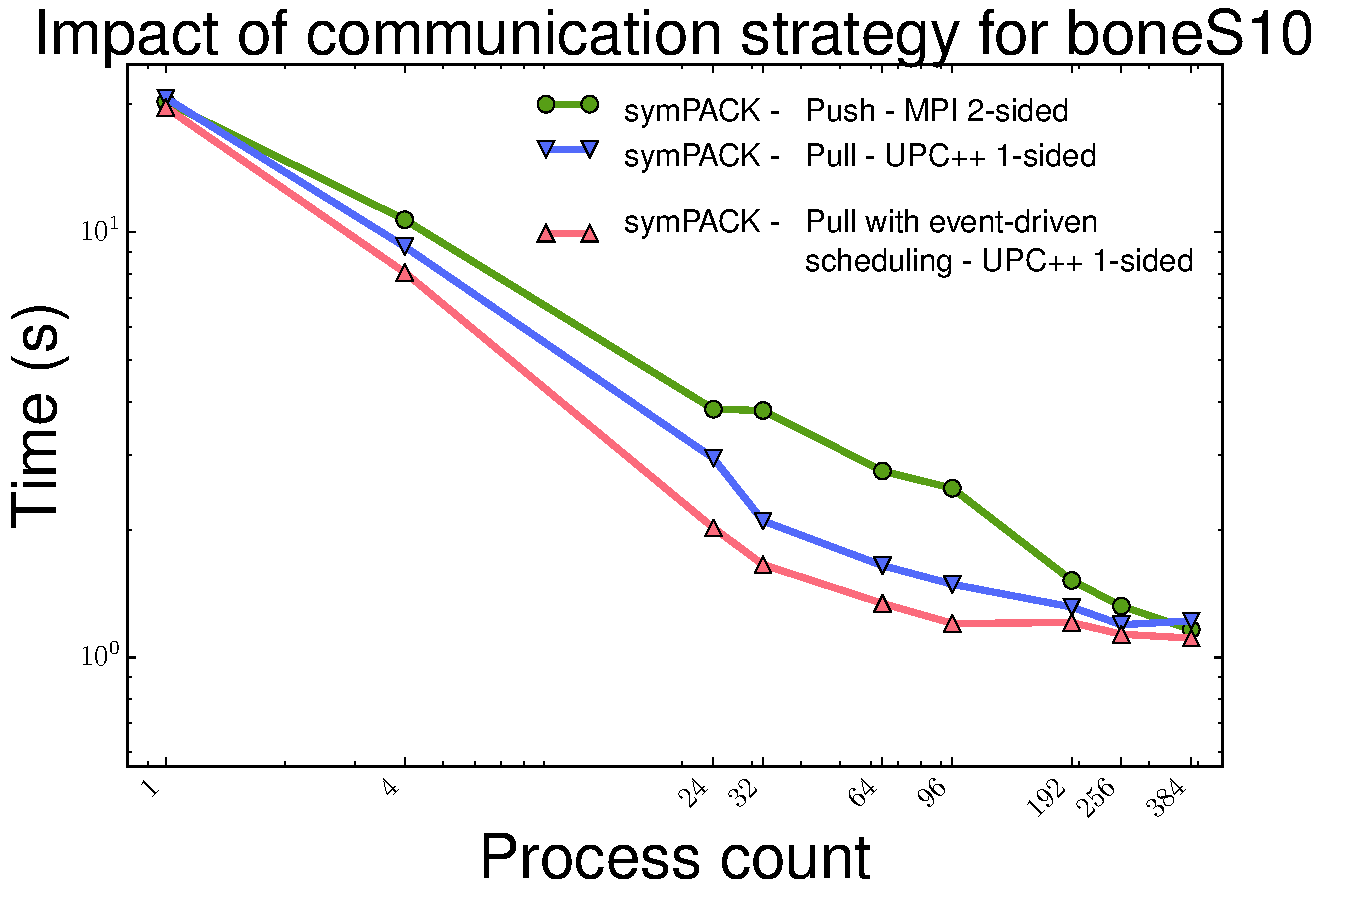
\includegraphics[width=3in]{projects/2.3.1-PMR/2.3.1.14-UPCxx-GASNet/ss_boneS10_comm.pdf}
  }
  \subfloat[Strong scaling of symmetric solvers\newline(Factorization time only)]{
    \label{fig:sympack:scaling}
	  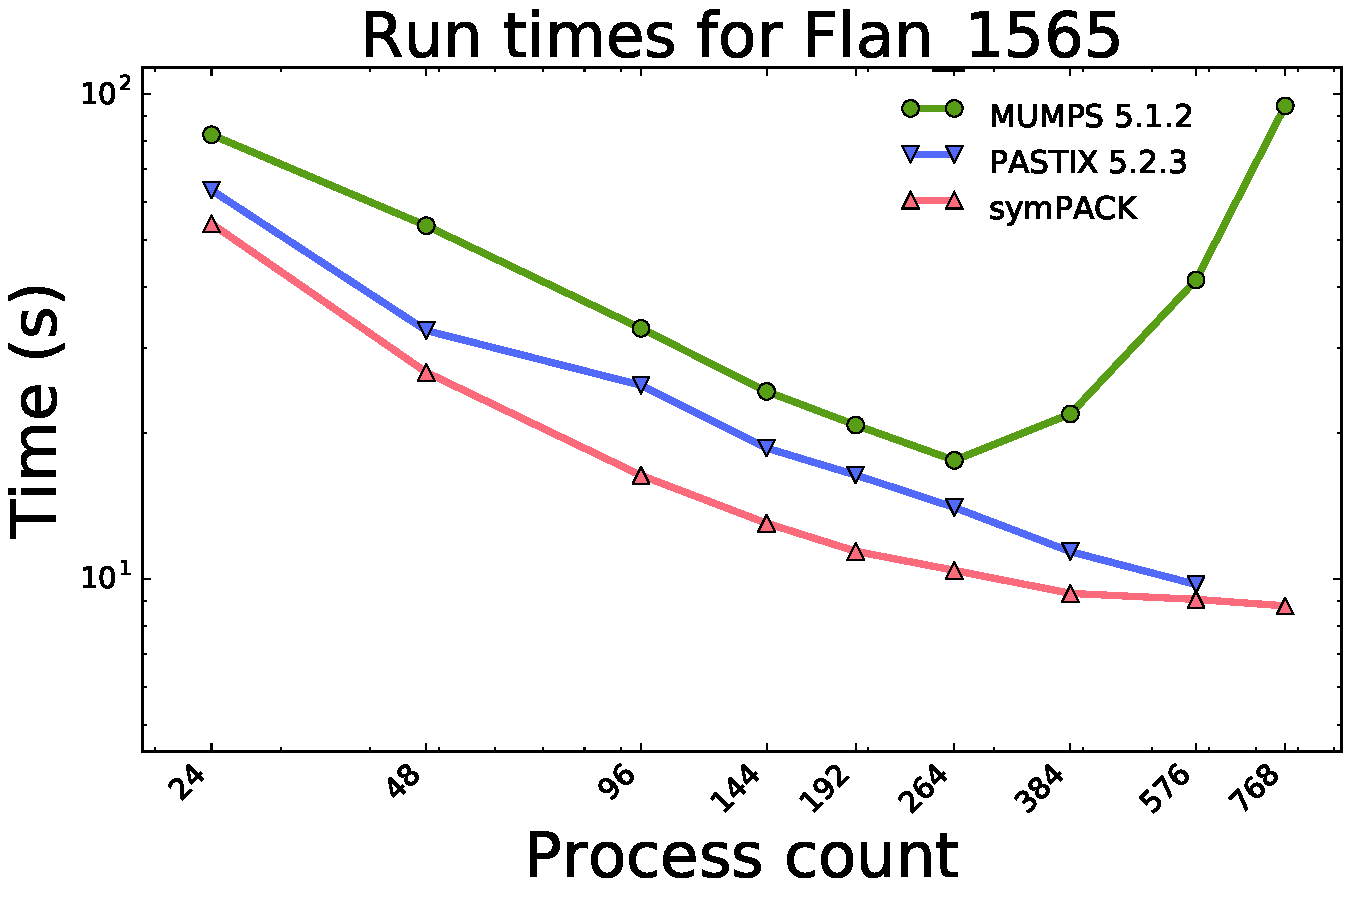
\includegraphics[width=3in]{projects/2.3.1-PMR/2.3.1.14-UPCxx-GASNet/ss_Flan_1565_complex.pdf}
  }
  \caption{\label{fig:sympack-perf}\textbf{Performance of the symPACK solver using UPC++ V1.0} }
\end{figure}



The first experiment, depicted in Fig.~\ref{fig:sympack:comm} compares the performance of three implementations of symPACK:
\begin{itemize}
  \item a \textbf{Push} strategy (the sender ``pushes'' the outgoing message
as soon as possible) using non-blocking MPI two-sided messages,
  \item a \textbf{Pull} strategy (sender ``notifies'' with RPC, receiver RMA gets when ready) using one-sided UPC++ RPC and RMA get,
  \item the same \textbf{Pull} strategy using one-sided UPC++ RPC and RMA get, combined with an event-driven dynamic scheduling policy.
\end{itemize}
UPC++ allows symPACK to implement an efficient Pull strategy using one-sided operations in a simple and efficient fashion.
This implementation surpasses the performance of the original MPI two-sided variant.
Fig.~\ref{fig:sympack:scaling} compares the strong scalability, on NERSC Edison, of symPACK with other state-of-the-art solvers
for sparse symmetric matrices. symPACK can be seen to significantly outperform
the other solvers on this particular problem, a trend which can be observed on most matrices from the SuiteSparse
matrix collection.

%Figure~\ref{fig:sympack-perf} illustrates the benefits of the PGAS model implemented by UPC++ (Mathias' results) .


% Figure~\ref{fig:dht-perf} illustrates the benefits of UPC++'s remote atomics capability with a distributed hash table implementation.
% \begin{figure}[htb]
	% \centering
	% \includegraphics[width=6in]{dht-perf}
	% \caption{\label{fig:dht-perf} {\bf CAPTION GOES HERE STEVE} }
% \end{figure}



\paragraph{Next Steps}


Our next efforts are:
\begin{enumerate}
\item \textbf{Team-aware APIs:} Teams are a mechanism for grouping ranks.
Team-aware APIs  will be developed to enable teams to be used not only in
collective communication (see below) but also in distributed objects,
and certain modes of accessing global shared storage.

\item \textbf{Support for non-blocking collectives:} UPC++ supports a small number
of collectives, and this set will be expanded to accommodate the needs of our
application partners. Support for teams will also be included.
	
	
\end{enumerate}

\newpage
\subsubsection{\stid{1.16} SICM}
\paragraph{Overview} The goal of this project is to create a universal interface for discovering, managing and sharing within complex memory hierarchies. The result will be a memory API and a software library which implements it. These will allow operating system, runtime and application developers and vendors to access emerging memory technologies. The impact of the project will be immediate and potentially wide reaching, as developers in all areas are struggling to add support for the new memory technologies, each of which offers their own programming interface. The problem we are addressing is how to program the deluge of existing and emerging complex memory technologies on HPC systems. This includes the MCDRAM (on Intel Knights Landing), NV-DIMM, PCI-E NVM, SATA NVM, 3D stacked memory, PCM, memristor, and 3Dxpoint. Also, near node technologies, such as PCI-switch accessible memory or network attached memories, have been proposed in exascale memory designs. Current practice depends on ad hoc solutions rather than a uniform API that provides the needed specificity and portability. This approach is already insufficient and future memory technologies will only exacerbate the problem by adding additional proprietary APIs. Our solution is to provide a unified two-tier node-level complex memory API. The target for the low-level interface are system and runtime developers, as well as expert application developers that prefer full control of what memory types the application is using. The high-level interface is designed for application developers who would rather define coarser-level constraints on the types of memories the application needs and leave out the details of the memory management. The low-level interface is primarily an engineering and implementation project. The solution it provides is urgently needed by the HPC community; as developers work independently to support these novel memory technologies, time and effort is wasted on redundant solutions and overlapping implementations. Adoption of the software is focused on absorbtion into existing open source projects such as hwloc, Umpire, CLANG/LLVM, OpenMP, and Jemalloc.
\begin{itemize}
\item  Low-Level Interface: Finished refactor of low-level interface supporting memory arenas on different memory types. Added initial support for Umpire, OpenMP. Reviewing features need to fully support these runtimes. SICM now supports Intel Optane memory, the first NVM memory that can be used as an extension of traditional DRAM memory.
Pull requests have been developed for OpenMP/CLANG/LLVM and Umpire. the patches to Clang/LLVM/OpenMP turn OpenMP memory spaces in OpenMP 5.x into SICM library calls in the LLVM/OpenMP runtime. The same codepath that supports memkind library was refactored to support multiple custom memory allocators – more general than just SICM support.
SICM currently supports "pragma openmp allocate" with  memory types: omp_ (default, large_cap, const, high_bw, low_lat ) _mem_spaces and supports KNL, Optane, testing on Sierra/Summit.

\begin{itemize}
\item  High-Level Graph Interface: Metall is a persistent memory allocator designed to provide developers with an API to allocate custom C++ data structures in both block-storage and byte- addressable persistent memories (e.g., NVMe and Intel Optane DC Persistent Memory) beyond a single process lifetime. Metall relies on a file-backed mmap mechanism to map a file in a filesystem into the virtual memory of an application, allowing the application to access the mapped region as if it were regular memory which can be larger than the physical main-memory of the system.
\item Analysis: 
SICM has employed application profiling and analysis to direct data management across complex memory hierarchy, the team extended the SICM high-level interface with application-directed data tiering based on the MemBrain approach which is more effective than an unguided first touch policy.  The impact of using different data features to steer hot program data into capacity-constrained device tiers was modeled.
\end{itemize}
\paragraph{Next Steps}
\begin{itemize}
\item  Low-Level Interface: Focus on performance of support for runtimes and adding feature requested to support Umpire, OpenMP and MPI and address the slow move pages implementation in the Linux kernel – (collaboration with RIKEN). Test with proxy applications for functionality and correctness. Investigate Linux kernel modifications for page migration in collaboration with ECP project Argo 2.3.5.05 and RIKEN research center in Japan, on-going. Start collaborating with applications to enable use of heterogenous memory on ECP target platforms. Additionally, the team needs to finalize the memory topology discover with the hwloc team.
\item For the analysis work the team will extend and hardend the tools for guiding application memory management and investigate feature categories to classify objects associated with different features such as size, type, allocation time, etc to guide data placement.
\item For the Metall high-level interface we plan to continue outreach to ExaGraph to store graph data as well as other intermediate data into PM leveraging Metall. We also plan to support UMap (user-level mmap library in Argo PowerSteering project) underneath Metall to enhance its performance and capability.
\end{itemize}



\newpage
\subsubsection{\stid{1.17} Open MPI for Exascale (OMPI-X)}\label{subsubsect:openmpi}

%% {\itshape

%% 	\begin{enumerate}
%% 	\item Rename this file to your project WBS-projectname.tex, for example 2.3.3.01-XSDK4ECP.tex.
%% 	\item Complete this template for your project.  Limit your text to two pages, not counting citations.
%% 	\item Please avoid changing the content of main.tex.
%% 	\item Put any references in a .bib file with the same root name, for example 2.3.3.01-XSDK4ECP.bib.
%% 	\item Remember to include any image files you reference in your text.
%%     \item The files 2.3.3.01-XSDK4ECP.tex, 2.3.3.01-XSDK4ECP.bib and xSDK-diagram.jpeg are included as examples for your reference.  You can remove them from what you upload.
%% 	\end{enumerate}
%% }

\paragraph{Overview}
%% \textit{Provide an overview of your project.  You might find that the introductory text from your Fall 2017 Project Summary \url{https://confluence.exascaleproject.org/display/1ST/Fall+2017+ECP+ST+Project+Summaries} useful as a starting draft.}

The OMPI-X project ensures that the Message Passing Interface (MPI)
standard, and its specific implementation in Open MPI meet the needs
of the ECP community in terms of performance, scalability, and
capabilities or features. MPI is the predominant interface for
inter-process communication in high-end computing.  Nearly all of the
ECP application (AD) projects (93\%~\cite{Bernholdt:2018:SMU-tr})
and the majority of software technology (ST) projects
(57\%~\cite{Bernholdt:2018:SMU-tr}) rely on it.
%% Since its
%% inception, the MPI standard has evolved to address the changing needs
%% of massively parallel libraries and applications as well as the
%% systems on which they are run.
With the impending exascale era, the
pace of change and growing diversity of HPC architectures pose new
challenges that the MPI standard must address.  The OMPI-X project is
active in the MPI Forum standards organization, and works within it to
raise and resolve key issues facing ECP applications and libraries.

Open MPI is an open source, community-based implementation of the MPI
standard that is
%% freely available, and
used by a number of prominent
HPC vendors as the basis for their commercial MPI offerings.  The
OMPI-X team is comprised of active members of the Open MPI community,
with an extensive history of contributions to this community.
%% the development and
%% maintenance of the library.
The OMPI-X project focuses on prototyping
and demonstrating exascale-relevant proposals under consideration by
the MPI Forum, as well as improving the fundamental performance and
scalability of Open MPI, particularly for exascale-relevant platforms
and job sizes.  MPI users will be able to take advantage of these
enhancements simply by linking against recent builds of the Open MPI
library.

Without the OMPI-X project, there will be less competition and less
innovation in addressing the needs of ECP users in the critical area
of scalable, performant, and expressive exascale-quality inter-process
communication capabilities.

\paragraph{Key  Challenges}
%% \textit{Describe what is hard to do, why it is challenging.}
A number of aspects of ``exascale'' levels
of computing pose serious challenges to the ``tried and true'' message
passing model presented by MPI and its implementations, including Open
MPI.
%
Keeping pace with changes in HPC architecture is a major challenge.
The MPI ecosystem (the standard and its implementations) needs to
evolve to address challenges
%% on the programming side
driven by
architectural change, as well as taking advantage of new features and
capabilities.
%
As applications and libraries
%% they rely on
build up to exascale,
%% levels of computing and beyond,
the number of nodes, processes, and
threads required will rise significantly, whereas other key resources,
such as memory tend to go \emph{down} on a per-node, -process, or
-thread basis.  This emphasizes the importance of scalability in terms
of both performance and resource utilization.
%% to allow MPI to scale to
%% meet those needs.
%
Finally, we must work within the much larger and broader MPI
community to find approaches to address these challenges which do not
adversely impact the capabilities, performance, or scalability for
other users of MPI and Open MPI.

\paragraph{Solution Strategy}
%% \textit{Describe your basic strategy for addressing the challenges.}
The OMPI-X project is working across a number of fronts to address
these challenges.

\emph{Runtime Interoperability for MPI+X and Beyond} MPI is
increasingly being used concurrently with other runtime environments.
This includes both ``MPI+X'' approaches, where X
%% , in the ECP
%% environment, X
is most often a threading model, such as OpenMP, as
well as the use of multiple inter-process runtimes within a single
application.  Concerns include awareness of other runtimes,
cooperative resource management capabilities, and ensuring that all
concurrently active runtimes make progress.  We will develop APIs and
demonstrate capabilities for interoperability in both MPI+X and
multiple inter-process runtime situations.

\emph{Extending the MPI Standard to Better Support Exascale
Architectures} The MPI community is considering for standardization a
number of ideas that 
%% A number of ideas under consideration by the MPI
%% community for standardization
are particularly important to supporting
the architectural and system size characteristics anticipated for
exascale.  ``Finepoints'' and ``Endpoints''
%% are approaches to
deal
with the growing use of threading for node-level concurrency, in
combination with MPI.  ``Sessions'' increases the flexibility of MPI
semantics in a number of areas, which in turn can open opportunities
for enhanced scalability, as well as easier support for
multi-component applications such as coupled multi-physics
simulations.  We will develop prototype implementations and work with
ECP teams to evaluate the ability of these approaches to address ECP
requirements in order to facilitate the standardization process.

\emph{Open MPI Scalability and Performance} As we push the scale of
both hardware and applications, we stress MPI implementations and
expose areas that need to be improved in order to improve scalability.
OMPI-X is targeting memory usage within Open MPI, as well as remote
memory access (RMA), tag matching, and other areas, for improvements
in both scalability and performance.

\emph{Supporting More Dynamic Execution Environments} We are
developing and implementing strategies to help MPI applications
better deal with topological process layout preferences
%% as well as
%% responding to
and contention in the network.

\emph{Resilience in MPI and Open MPI} Concerns about system and
application resilience increase as either scales in size.
%% (number of
%% components or MPI ranks).
We will provide implementations of the
User-Level Fault Mitigation (ULFM) and ReInit proposals currently
under discussion within the MPI Forum, as well as demonstrations of
their use, in order to help drive standardization discussions, and to
help ECP team understand how they can take advantage of these
capabilities to improve the resilience of their libraries and
applications.

\emph{MPI Tools Interfaces}  Several interfaces within the
MPI standard are primarily used to support performance and
correctness tools.
%% of various kinds.
The MPI Forum is in the process
of making significant revisions and extensions to these interfaces.
We will track the discussions in the Forum and provide prototype
implementations within Open MPI to facilitate evaluation and provide
feedback.
%% on the standardization discussions.
We will work with the
ECP community, including tool developers, to make additional data
available through the MPI\_T interface.

\emph{Quality Assurance for Open MPI}  We are enhancing the
Open MPI testing infrastructure, adding tests to reflect ECP
requirements, and instantiating routine testing on systems of
importance to ECP.

\paragraph{Recent Progress}
%% \textit{Describe what you have done recently.  It would be good to
%% have some kind of figure or diagram in this section.}
The survey of MPI usage conducted last year continues to have impact
in the community.  In an article in The Next Platform in August
described our technical report \cite{Bernholdt:2018:SMU-tr} as a
``must read''.  Additionally, the MPI community, led in part by OMPI-X
team members, has launched a survey to obtain input from the broader
international MPI user community.

During the past year, we have ramped up our work in runtime
interoperability for ``MPI+X'' programming approachs.  We have
prototyped a capability to coordinate placement of ranks and threads
between MPI and OpenMP which cannot be achieved by ``standard''
methods.  This work has garnered significant interest in the community
and we forsee these activities expanding beyond our original
expectations.

%% We have delivered an implementation of the User-Level Fault Mitigation
%% (ULFM) resilience approach, which are under consideration by the MPI
%% Forum for inclusion in the standard.  ULFM provides the basic building
%% blocks for cheap, tailored recovery capabilities within applications
%% and libraries using MPI.  ULFM imposes no overhead on raw
%% communication performance on ECP-relevant hardware.  We are now
%% working with several application teams to demonstrate the capabilities
%% it provides.

%% \begin{wrapfigure}{r}{4in}
%% \begin{minipage}[c]{2in}
%% \vspace{0pt}
%% 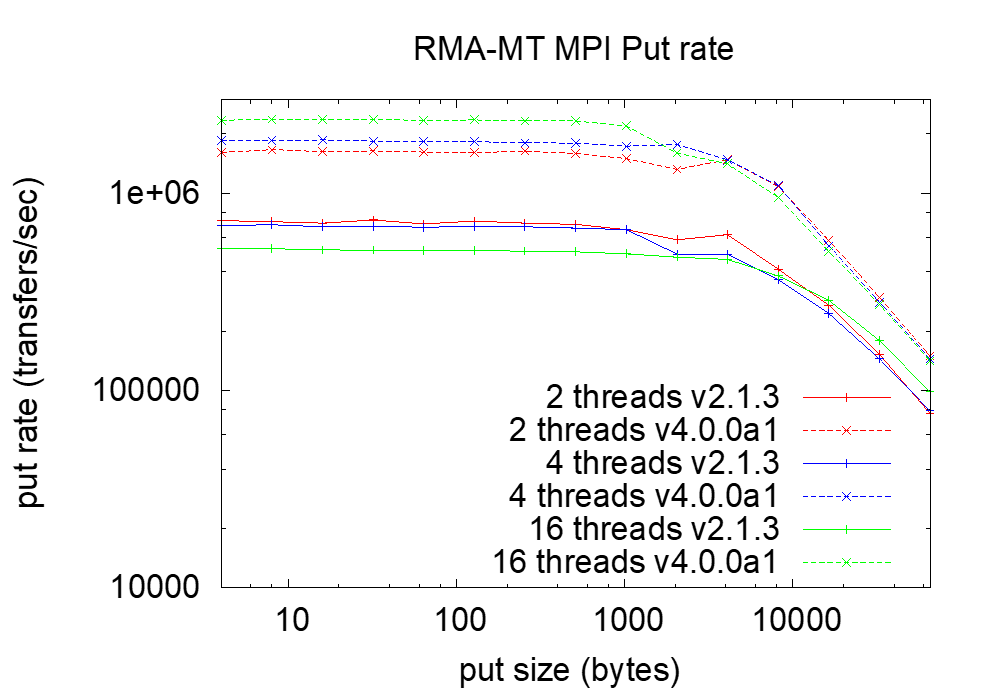
\includegraphics[width=\textwidth]{projects/2.3.1-PMR/2.3.1.11-OMPI-X/pritchard-rma-mt-put-rate.png}
%% \end{minipage}
%% \begin{minipage}[c]{2in}
%% \vspace{0pt}
%% 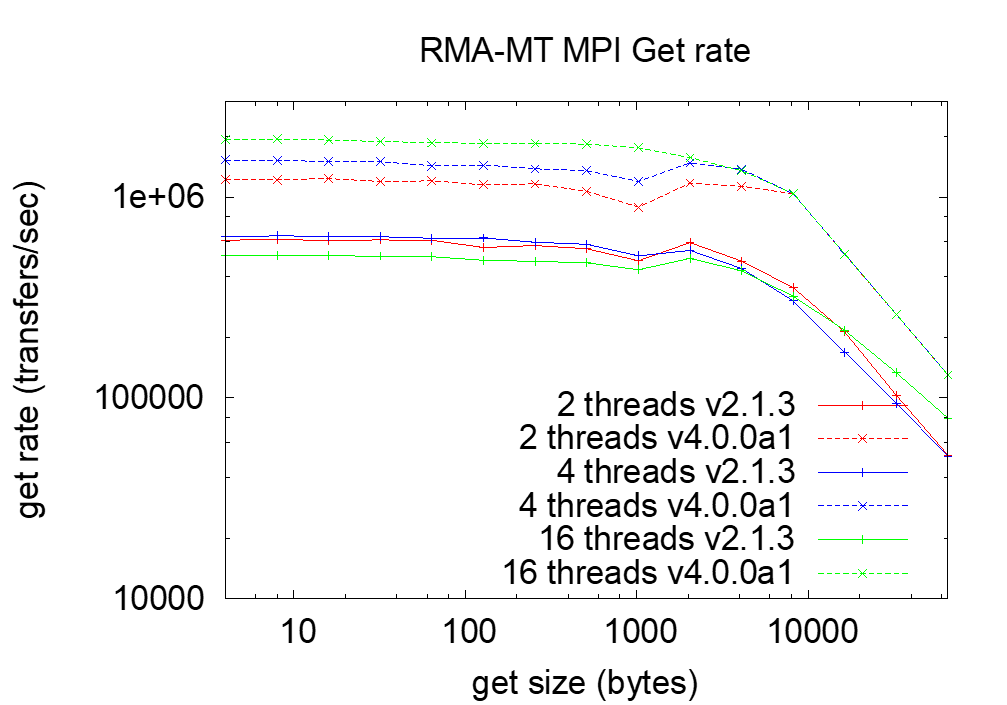
\includegraphics[width=\textwidth]{projects/2.3.1-PMR/2.3.1.11-OMPI-X/pritchard-rma-mt-get-rate.png}
%% \end{minipage}
%% \caption{Comparison of put (left) and get (right) RMA performance in a
%% multi-threaded context for Open MPI.  Recent OMPI-X contributions are
%% reflected in version 4.0.0a1 (top group of lines), in comparison with
%% v2.1.3.}
%% \label{fig:ompix-rma}
%% \end{wrapfigure}

The OMPI-X team has been active in the MPI Forum, driving
conversations about the Endpoints and Finepoints approaches to
supported threaded programming, and the Sessions concept, which will
improve the scalablity and flexibility of MPI.  Our prototype
Finepoints implementation shows improvements of 25\% in communicaton
time and 5\% in total runtime for an ECP mini-application.  New
aggregation techniques have been shown to provide 445\% increase in
communication bandwidth in certain cases.

The OMPI-X team is also active in other areas of the evolution of the
MPI standard. We have been driving development of the ``Sessions''
concept, will allow increased scalability in MPI applications and
implementations, as well as greater flexibility.
%
We are also tracking work on the PMPI tools interface replacement and
the enhancements to the MPI\_T tools interface.  We are working with
other members of the community to bring production-quality
implementations of these updated interfaces to Open MPI.

In the resilience area, we continued prior work on the User-Level
Fault Mitigation (ULFM) capability, fully integrating it into Open MPI
for the v4 release.  We also continue to pursue the ``Reinit'' fault
tolerance approach, completing the initial API design and plan for
implementation within Open MPI.

Behind the scenes of the Open MPI implementation, we are pursuing
efforts to improve performance and scalability, take full advantage of
the increasingly complex and sophisticated memory architectures that
are becoming available at the node level, and providing increased
topology and congestion awareness within the library.  We have made
improvements in RMA performance, which allows better scaling and
provides out-of-the-box performance in Open MPI which is comparable to
highly-tuned vendor implementations.  We have prototyped improved an
message matching implementation which improves matching performance by
up to 2x and saves significantly (1 GB) in memory, providing an
improvement in total runtime for on applicaton of 6\%.  We have also
worked to improve the MPI startup process by up to 5x in some
configurations.  And we have begun baselining memory utilization
in order to analyze and improve memory scalability.

%% We expect to be working on scalability and performance of Open MPI
%% throughout the project, but some early successes have been
%% demonstrated.  We have improved the RMA implementation so achieve
%% performance levels comparable to those obtained only by high tuned
%% implementations by vendors and significantly improved their
%% performance in multi-threaded contexts (Fig.~\ref{fig:ompix-rma}).  We
%% have also been able to improve message matching by up to 2$\times$
%% generally, and up to 45$\times$ on Intel Xeon Phi processors, and we
%% have made significant improvement to performance when MPI is used in a
%% multi-threaded environment.

%% %% Early work with the prototype implementation of Finepoints shows
%% %% improvements of 25\% in communication costs and 5\% in overall
%% %% execution time for one ECP mini-app.
%% %
%% Open MPI support for the MPI\_T interface has been extended~\cite{icl:957} to
%% provide a set of low-level counters to present a more detailed performance
%% characteristics map to tools and to users.
%
Finally, we continue to build out the MTT testing infrastructure and
continuous integration testing capabilities to provide better testing
capabilities for ECP-relevant platforms, including Summit at ORNL.

\paragraph{Next Steps}
%% \textit{Describe what you are working on next.}
We are making progress across multiple fronts, some of which has been
described above.  In FY19, we expect to continue our efforts on MPI+X
interoperability, pushing forward the Finepoints and Sessions
prototypes and standards proposals, as well as implementations of the
PMPI replacement and MPI\_T improvements.  We will also continue our
internal improvements in performance, scalability, and capabilities to
take maximum advantage of modern system capabilities. We are
tentatively planning to merge 2.3.1.15-Qthreads into OMPI-X in the
second phase of ECP ST activities due to the close technical and
personnel connections.
\subsubsection{\stid{1.15} Enhancing Qthreads for ECP Science and Energy Impact} 


\paragraph{Overview} 

``Enhancing Qthreads for ECP Science and Energy Impact'' is a project that aims to improve the performance of applications that use multithreading with communication, e.g., MPI.  Most ECP applications are using this combination of programming models, with the Kokkos or RAJA performance portability libraries and/or the OpenMP API for multithreading.  This project supports the Kokkos ECP software project and OpenMP from the underlying runtime layer to deliver thread-scalable performance to those applications.  To that end, our projects is developing techniques to incorporate support for better network concurrency into the multithreading runtime system.

\paragraph{Key  Challenges}
Our project addresses the challenge of scalably coupling multithreaded parallelism on the many-core node with communication such as MPI, which has traditionally performed poorly in multithreaded mode.  The key challenge arises when multiple threads make communication calls, and those calls must be serviced by the MPI implementation and NIC.  Existing solutions, such as MPI\_THREAD\_MULTIPLE, are often plagued by synchronization overheads.  Even the best vendor MPI implementations incur high overheads when the number of threads exceeds the number of hardware contexts in the NIC. 
While current mechanisms are insufficient even for today's systems, emerging interconnect technologies expose even more network parallelism that must be exploited to maximize performance for Exascale.

\paragraph{Solution Strategy}

Unlike previous approaches, we attack the problem not only from the communication side (MPI), but with assistance from the multithreading runtime system.  Our work adds capabilities to enable the runtime system to identify and optimize for tasks that use communication, distinct from tasks that perform only local computation.  We use the Qthreads runtime~\cite{wheeler2008qthreads}, a scalable, event-driven library for node-level task parallelism, to implement our solution.  This work requires cooperation with a communication library that can scalably process communications operations coming from the runtime system.  For this purpose, we pair Qthreads with the new “FinePoints" library for threaded MPI execution developed in the OMPI-X ECP project.

Developed at Sandia Labs since 2007, Qthreads serves as a back-end for Kokkos and the Cray Chapel language, as well as providing a portable native C API. Complementary to the current ECP project focusing on the coupling of the runtime with communication, development of Qthreads core capabilities is part of the NNSA ASC system software portfolio and has also been part of sponsored vendor collaborations and LDRD projects.  In addition, the techniques developed in this project will be the subject of tech transfer efforts to OpenMP and MPI.  The project technical lead is chair of the OpenMP Subcommittee on Task Parallelism, and one of the other technical experts on the project is a key contributor to the MPI Forum and the OMPI-X ECP project that is enhancing the open-source Open MPI implementation of MPI for exascale.  We are leveraging the work of that project, and synergies between Qthreads and the OpenMP and Kokkos tasking models.


\paragraph{Recent Progress}

Recently, we added the optional network task annotation to task definitions in Qthreads, allowing the identification of communication tasks to the runtime system.  We also demonstrated successful coupling of Qthreads with the MPI FinePoints library.  FinePoints uses a partitioned buffer to collect the contributions of the various tasks executing on the runtime’s threads.  Using only atomics rather than heavyweight locks keeps overhead costs low compared to existing methods like MPI\_THREAD\_MULTIPE, and unlike the Endpoints proposal, the MPI rank space does not expand with the use of more threads.  We ported FinePoints benchmark code to use Qthreads as the multithreading library instead of OpenMP and compared to the performance of the two configurations, shown in Figure~\ref{fig:qthreads-finepoints-graph}. The observed equivalence in performance justifies our use of Qthreads as a proxy for OpenMP, wherein Qthreads can be used for ease of rapid prototyping of new capabilities with eventual tech transfer back to OpenMP.  These results also serve as baselines to measure the performance of our further optimizations against.  Finally, we made an initial port of the miniGhost stencil mini-app to use FinePoints with Qthreads to confirm portability beyond benchmarks.  Tuning of that mini-app is currently work in progress.

\begin{figure}[htb]
	\centering
	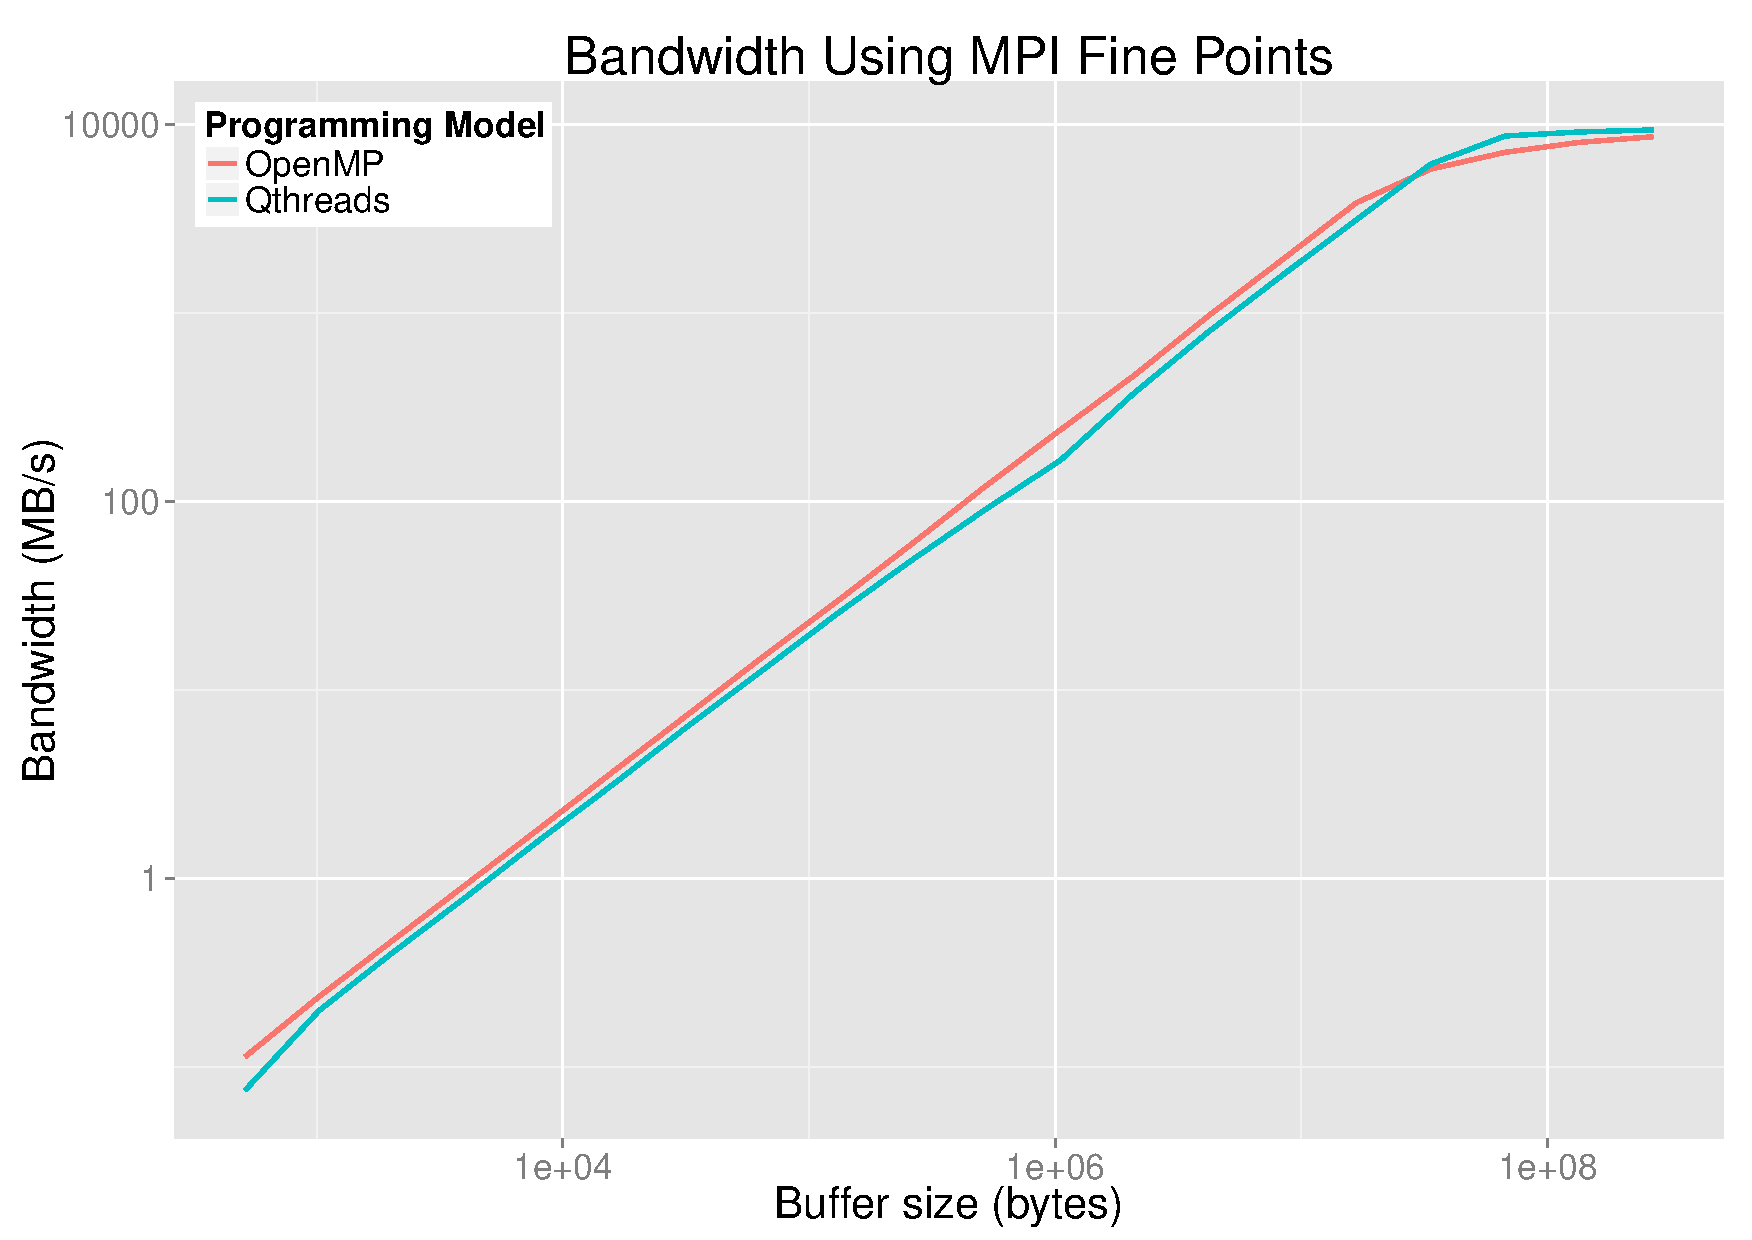
\includegraphics[width=6in]{projects/2.3.1-PMR/2.3.1.17-OMPI-X/FinePointsBW-QtOmp.pdf}
	\caption{\label{fig:qthreads-finepoints-graph}This graph shows the performance of Qthreads and OpenMP paired with the FinePoints library for multithreaded MPI.  The x-axis varies the buffer sizes transferred in each experiment in the series, and the y-axis shows the network bandwidth achieved.  The similar performance of Qthreads and OpenMP justifies use of the former as a suitable proxy for the latter, with the advantage of flexibility for rapid prototyping of new runtime system techniques.}
\end{figure}

Progress from the project through the end of FY18 was incorporated in the Fall 2018 Qthreads release~\cite{qthreads-github}.  We also published a paper at the SC18 Correctness Workshop that showed the feasibility of model checking for correctness testing of tasking runtimes (with Qthreads as the runtime used for demonstration)~\cite{evans2018qthreads-model}.  This work emphasizes the importance of software robustness and the need to work toward systematic rather than ad hoc testing of system software such as threading runtimes.

\paragraph{Next Steps}

We plan to investigate several possible optimizations of the Qthreads runtime improvements in conjunction with FinePoints and the OpenMPI implementation. FinePoints is natively available as an extension of OpenMPI or as a library layered on top of any MPI implementation. We will evaluate new runtime scheduling strategies based on the categorization of network and non-network tasks enabled by our task tagging scheme. We have also begun work on an effort to integrate Qthreads as a threading layer for OpenMPI in place of pthreads. Since the Argobots team at Argonne National Laboratory has been working in a similar vein in MPICH, we will hold a working session with them in 2019 to work toward making both user-level threading libraries compatible with both MPI implementations.

Based on the close ties between the Qthreads project and the OpenMPI-X project, we have asked that the Qthreads project become a part of the OpenMPI-X as part of the project reorganization for the second phase of ECP.


\newpage
\subsubsection{\stid{1.18} ISC4MCM (RAJA)} 

\paragraph{Overview.} 
The Integrated Software Components for Managing Computation and Memory 
Interplay at Exascale (ISC4MCM) project is providing software libraries that 
enable application and library developers to meet advanced architecture 
portability challenges. The project goals are to enable writing performance 
portable computational kernels and coordinate complex heterogeneous memory 
resources among components in a large integrated application. These 
libraries enhance developer productivity by insulating them from much of the 
complexity associated with parallel programming model usage and 
system-specific memory concerns.

The software products provided by this project are three complementary and 
interoperable libraries:
\begin{enumerate}
\item {\bf RAJA:} Software abstractions that enable C++ developers to write
  performance portable (i.e., single-source) numerical kernels (loops). 
\item {\bf CHAI:} C++ ``managed array'' abstractions that enable transparent
  and automatic copying of application data to execution memory spaces at run
    time as needed based on RAJA execution contexts.
\item {\bf Umpire:} A portable memory resource management library that provides
  a unified high-level API for resource discovery, memory provisioning,
    allocation, access, operations, and introspection.
\end{enumerate}

Capabilities delivered by these software efforts are needed to manage the
diversity and uncertainty associated with current and future HPC architecture
design and software support. Moving forward, ECP applications and libraries 
need to achieve performance portability: without becoming bound to particular
(potentially-limiting) hardware or software technologies, by insulating 
numerical algorithms from platform-specific data and execution concerns, and 
without major disruption as new machine, programming models, and vendor
software become available.

These libraries in development in this project are currently used in production
ASC applications at Lawrence Livermore National Laboratory (LLNL). They are
also being used or being explored/adopted by several ECP application and
library projects, including: LLNL ATDM application, GEOS (Subsurface), SW4
(EQSIM), MFEM (CEED co-design), and SUNDIALS.

The software projects are highly-leveraged with other efforts. Team members
include: ASC and ATDM application developers, ASD tool developers, university
collaborators, and vendors. This ECP ST project supports outreach to the ECP
community and collaboration with ECP efforts.

\paragraph{Key Challenges.}

The main technical challenge for this project is enabling production
applications to achieve performance portability in an environment of rapidly
changing, disruptive HPC hardware architecture design. Typical large
applications contain $O(10^5) - O(10^6)$ lines of code and $O(10K)$ loop
kernels. The codes must run efficiently on platforms ranging from laptops to
commodity clusters to large HPC platforms. The codes are long-lived and are
used daily for decades, so they must be portable across machine generations.
Also, the codes are under continual development, with a steady stream of new
capabilities added throughout their lifetimes -- continual validation and
verification is essential, which precludes substantial rewrites from scratch.
Lastly, the complex interplay of multiple physics packages and dozens of
libraries makes it so that the data required for the full set of components
needed for a given simulation may not fit into a single system memory space. To
advance scientific computing capabilities, applications must navigate these
constraints while facing substantial hardware architecture disruption along the
road toward Exascale computing platforms. 

While the software provided by this project has a substantial user base at
LLNL, achieving broader adoption in the ECP (projects without LLNL involvement,
in particular) is another challenge. The software efforts are funded almost
entirely by LLNL programs and the majority of their developers work on LLNL
application projects. So resource limitations is a key issue.

\paragraph{Solution Strategy.}

The software libraries in this project focus on encapsulation and 
application-facing APIs to insulate users from the complexity and 
challenges associated with diverse forms of parallelism and heterogeneous 
memory systems. This approach allows users to exploit new capabilities 
with manageable rewriting of their applications.

RAJA provides various C++ abstractions for parallel loop execution. It
supports: various parallel programming model back-ends, such as OpenMP 
(CPU multithreading and target offload), CUDA, Intel Threading Building Blocks,
etc.; loop iteration space and data view constructs to reorder, 
aggregate, tile, and partition loop iterations; complex loop kernel 
transformations for optimization, such as reordering loop nests, fusing 
loops, etc. RAJA also supports portable atomic operations, parallel scans, 
and CPU and GPU shared memory. After loops have been converted to RAJA, 
developers can explore implementation alternatives via RAJA features without 
altering loop kernels at the application level.

CHAI provides C++ ``managed array'' abstractions that automatically copy 
data to execution memory spaces as needed at run time based on RAJA execution 
contexts. Access to array data in loop kernels looks the same as when using
traditional C-style arrays.

Umpire provides a portable API for managing complex memory resources by 
providing uniform access to other libraries and utilities that provide
system-specific capabilities. Umpire decouples resource allocation from 
specific memory spaces, allocators, and operations. The memory introspection 
functionality of Umpire enables applications and libraries to make memory 
usage decisions based on allocation properties (size, location, sharing 
between packages, etc.)

All three software libraries are open source and available on
GitHub~\cite{RAJA-github, CHAI-github, Umpire-github}. There they provide
regular software and documentation releases. Each project has dedicated email
lists, issue tracking, test suites, and automated testing.

\paragraph{Recent Progress}

In FY18, CHAI and Umpire have been released as open source software projects
and they are now developed on GitHub Recent development has focused on 
user documentation and cleaner integration of these two libraries to give 
applications more flexible and easy access to their capabilities.

Many new features have been added to RAJA in FY18 to enable flexible
loop transformations for complex loop kernels via execution policies.
LLNL applications are assessing this new functionality now in a 
"pre-release" version; it will be generally available before the end of FY18.

The RAJA Performance Suite~\cite{RAJAPerf-github} was released and made 
available on Github in January 2018. The Suite is used to assess and track 
performance of RAJA across programming models and diverse loop 
kernels. It is also being used for compiler acceptance testing in the CORAL 
procurement and was prepared for use as a benchmark for the CORAL-2 procurement.

In 2018, the RAJA project expanded its visibility beyond DOE NNSA Labs. 
Recent presentations include a RAJA tutorial at the 2018 ECP Annual Meeting 
and an application use case study the 2018 NVIDIA GPU Tech Conference (GTC). 
Future tutorials are planned at 2018 ATPESC and GTC 2019. Also, a RAJA paper 
and $1/2$-day tutorial proposal were submitted to SC18.

\paragraph{Next Steps}

Our next efforts include:
\begin{enumerate}
\item {\bf Fill RAJA Gaps:} Not all features are available for all programming
  model back-ends; as models mature, such as OpenMP4.5, these gaps will be
    filled.
\item {\bf Expand RAJA User Guide and Tutorial:} Build example codes and user
  documentation for latest RAJA features and prepare for future tutorials
    (ATPESC 2018 and SC18).
\item {\bf Expand RAJA Performance Suite:} Include kernels that exercise more
  application use cases and RAJA features.
\item {\bf Focus RAJA Vendor Interaction:} Work with CORAL vendors to address
  issues as applications port to the Sierra platform at LLNL; establish early
    interactions with CORAL-2 vendors to ensure RAJA will be supported well on
    CORAL-2 systems.
\item {\bf Expand Umpire Capabilities:} Explore potential collaboration with
  relevant ECP efforts, such as SICM project.
\end{enumerate}
\subsubsection{\stid{1.18} Kokkos} 

\paragraph{Overview} 

The Kokkos C++ Performance Portability Ecosystem is a production-level solution for writing modern C++ applications in an hardware-agnostic way.
Started by Sandia National Laboratories, it is now supported by developers at the Argonne, Berkeley, Oak Ridge, Los Alamos and Sandia National Laboratories as well as the Swiss National Supercomputing (Centre).
It is now used by more than a hundred HPC projects, and Kokkos-based codes are running regularly at-scale on half of the top ten supercomputers in the world. 
The EcoSystem consists of multiple libraries addressing the primary concerns for developing and maintaining applications in a portable way.
The three main components are the Kokkos Core Programming Model, the Kokkos Kernels Math Libraries and the Kokkos Tools.
Additionally, the Kokkos team is participating in the ISO C++ standard development process, to get successful concepts from the Kokkos EcoSystem incorporated into the standard. 
Its development is largely funded as part of the Exascale Computing Project, with a mix of NNSA ATDM and Office of Science sources. 

 
\paragraph{Key Challenges}

One of the biggest challenges for the ExaScale supercomputing era is the proliferation of different computer architectures, and their associated mechanisms to program them.
Vendors have an incentive to develop their own models in order to have maximum freedom of exposing special hardware capabilities, and potentially achieve "vendor-lock-in".
This poses the problem for applications that they may need to write different variants of their code for different machines - an effort which can be simply not feasible for many of the larger application and library projects.

The Kokkos project aims at solving this issue by providing a programming solution which provides a common interface build upon the vendor specific software stacks.
There are a number of technical challenges associated with that. 
First an abstraction must be designed which is restricted enough to allow mapping to a wide range of architectures while allowing exploitation of all the hardware capabilities provided by new architectures. 
Secondly, the development of support for a new architecture may take significant resources. In order to provide a timely solution for applications in line with the availability of the machine, CoDesign collaborations with the vendors are critical.
At the same time software robustness, quality and interface stability is of utmost importance. 
In contrast to libraries such as the BLAS, programming models permeate the entire code base of an application, and are not isolated to simple call sites. 
API changes thus would require a lot of work inside of the users code base. 
A fourth challenge is that in order to debug and optimize the code base tools are required to gain insights into the application. 

Besides the technical challenges, 
a comprehensive support and training infrastructure is absolutely critical for a new programming model to be successful.
Prospective users must learn how to use the programming model, current users must be able to bring up issues with the development team and access detailed documentation, and the development team of the model must be able to continue technical efforts without being completely saturated with support tasks. 
The latter point became a significant concern for the Kokkos team with the expected growth of the user base through ECP.  
Already before the launch of ECP, there were multiple application or library teams starting to use Kokkos for each developer on the core team -- a level not sustainable into the future without a more scalable support infrastructure. 
This issue was compounded by the fact that Kokkos development was funded through NNSA projects, making it hard to justify extensive support for open science applications. 

\paragraph{Solution Strategy}

To address the challenges the Kokkos team is developing a set of libraries and tools which allow application developers to implement, optimize and maintain performance portable codes. 
At its heart the EcoSystem provides the Kokkos Core Programming Model.
Kokkos Core is a programming model for parallel algorithms that use many-core chips and share memory among those cores.
The programming model includes abstractions for frequently used parallel execution patterns, policies that provide details for how those patterns are executed, and execution spaces that denote on which execution agents the parallel computation is performed. 
Kokkos Core also provides fundamental data structures with policies that provide details for how those data structures are laid out in memory, memory spaces that denote in which memory the data reside, and data access traits conveying special data access semantics.
The model works by requiring that application development teams implement their algorithms in terms of Kokkos’ patterns, policies, and spaces. 
Kokkos Core can then map these algorithms onto the target architecture according to architecture-specific rules necessary to achieve best performance.

Kokkos Kernels is a software library of linear algebra and graph algorithms used across many HPC applications to achieve best (not just good) performance on every architecture. The baseline version of this library is written using the Kokkos Core programming model for portability and good performance. The library has architecture-specific optimizations or uses vendor-specific versions of these mathematical algorithms where needed. This reduces the amount of architecture-specific software that an application team potentially needs to develop, thus further reducing their modification cost to achieve “best in class” performance. 

Kokkos Tools is an innovative “plug in” software interface and a growing set of performance measurement and debugging tools that plug into that interface for application development teams to analyze the execution and memory performance of their software. Teams use this performance profiling and debugging information to determine how well they have designed and implemented their algorithms and to identify portions of their software that should be improved. Kokkos Tools interfaces  leverage the Kokkos Core programming model interface to improve an application developer’s experience dramatically, by forwarding application specific information and their context within the Kokkos Core programming model to the tools.

Kokkos Support addresses the challenges of establishing, growing and maintaining the user community.
First and foremost, it provides explicit means for supporting all DOE ECP applications. 
A main component of that is funding for local Kokkos experts at the Sandia, Oak Ridge, Argonne, Berkeley and Los Alamos laboratories which can serve as direct contacts for local applications and the users of the leadership computing facilities. 
Secondly, the project develops and maintains a reusable support infrastructure, which makes supporting more users scalable and cost effective. 

The support infrastructure consists of GitHub wiki pages for the programming guide and API reference, GitHub issues to track feature requests and bug reports, a Slack channel for direct user-to-user and user-to-developer communication, and tutorial presentations and cloud-based Kokkos hands-on exercises. 

The Kokkos Team is also actively engaging the ISO C++ Committee, where it provides about a third of the members interested in HPC.
This strong engagement enables the team to lead or contribute to numerous proposals.
Among those proposals the team leads are abstractions for multi dimensional arrays based on Kokkos View, atomic operations on generic types and linear algebra algorithms based on Kokkos Kernels, which cover not only the classic Fortran BLAS capabilities, but also batched BLAS and mixed precision linear algebra.
The team also has a central role in the primary proposal introducing heterogeneous computing into the C++ standard via the executors concept.

\paragraph{Recent Progress}

The Kokkos project now consists of an integrated developers team spanning five DOE National Laboratories.
In particular both NNSA and Office of Science funded developers are working based off the same task and code management system, use a shared slack channel, and attend a common weekly team meeting.
This ensures that no duplication of effort happens, and makes Kokkos a true inter laboratory project.

Kokkos is now used by many applications in production across the entire spectrum of DOE's super computers.
Support for current production platforms is mature and stable.
Work on supporting the upcoming ExaScale platforms has begun and initial capabilities for AMD GPUs and Intels GPUs are working.
On the AMD side this is despite the fact that full support was previously available, but had to be removed due to the deprecation of the underlying programming model by AMD.

Three Kokkos specific multi-day boot camps were organized with a total attendance on the order of 60 developers.
Additionally the team provided single day tutorials at numerous venues with several hundred attendees in aggregate.
The slack channel now sees daily questions from numerous users, and has attracted even vendor representatives who help answer machine specific questions.
The team finished developing a full API documentation as well as adding use case descriptions for common patterns found in applications.

At the C++ committee, the MDSpan proposal is now in wording review - meaning that the technical design is approved. 
MDSpan will be able to provide all the core capabilities of Kokkos\:\:View.
This includes compile and runtime extents, customizable layouts, and data access traits.
The extension to heterogeneous memory can be achieved by trivial extensions. 
Furthermore, the atomic\_ref proposal was voted into C++20.
This capability will provide atomic operations on generic allocations as powerful as Kokkos' atomic operations.
In particular it allows atomic operations on types independent of their size, and not just the ones native in the hardware.
A very recent development, is the proposal for linear algebra functions.
It entails functionality covering all of BLAS 1, 2, and 3, but extends it to any scalar types (including mixing of scalar types) and batched operations.
The proposal was approved by the relevant study groups, as well as the library evolution incubator group.
The Kokkos team was also able to gain co-authors from NVIDIA, Intel and AMD - providing significant support from the leading hardware vendors.

\paragraph{Next Steps}

The most pressing next task is to complete and then mature support for the upcoming ExaScale architectures.
Most of Kokkos's functionality is expected to be available by the end of FY20 for those systems, which will provide another year of time to mature the support before the first platforms will be delivered.

On the programming model evolution side, more explicit asynchronous capabilities including the creation of graphs of kernel launches is a high priority.

At the plumbing level, the team will start to replace some of the implementation level of Kokkos by the ISO C++ capabilities such as atomic\_ref and mdspan.

For Kokkos tools an upcoming capability will be the addition of autotuning tools. This will help with the increasingly difficult task of coming up with heuristics to determine good runtime settings for kernels on all the different architectures.

And last but not least, the team will work on getting the proposed new ISO C++ capabilities into the C++23 draft standard, so that they will be available to our users as a vendor provided capability during the lifetime of the first ExaScale platforms.

\newpage
\subsubsection{\stid{1.18} Runtime System for Application-Level Power Steering on Exascale Systems} 

\paragraph{Overview} 
Power remains a critical constraint for Exascale. As we design supercomputers at larger scales, power becomes an expensive and limited resource. Inefficient management of power leads to added operational costs as well as low scientific throughput. Although hardware advances will contribute a certain amount towards achieving high energy efficiency, they will not be sufficient, creating a need for a sophisticated system software approach. Significant advances in software technologies are thus required to ensure that Exascale systems achieve high performance with effective utilization of available power. Distributing available power to nodes while adhering to system, job and node constraints involves complex decision making in software. 

The ECP PowerSteering project is developing a \emph{job-level} power management runtime system that will optimize performance of Exascale scientific applications transparently under power and/or energy constraints. Existing research efforts, including Conductor and Adagio, are being actively integrated into Intel's GEOPM runtime system, an ongoing open source effort led by Intel. This integration expands GEOPM's capabilities with the latest research while providing a production-grade, industry-supported open source solution. By developing new platform plugins, this project also supports upcoming target platforms and paradigms for ECP beyond the Intel architectures, and incorporates task-based programming models such as Legion. By being both configurable and cross-platform, GEOPM will help applications achieve maximum performance under a power constraint. 

This project is essential for ECP because it enables Exascale applications to operate safely with optimal performance under power and energy constraints. This project is also essential for building a sophisticated hierarchical software stack proposed by the ECP Argo and ECP Flux projects. Additionally, the project fulfills an essential need for ECP by enabling vendor and academic collaborations that provide for accelerated adoption of best practices and better interoperability at scale.  By leveraging the GEOPM software developed in this project, compute centers can safely operate under power and energy constraints while maximizing performance and scientific throughput. 


\paragraph{Key Challenges}
Power management in software is challenging due to the dynamic phase behavior of applications, processor manufacturing variability, and the increasing heterogeneity of node-level components. While several scattered research efforts exist, a majority of these efforts are site-specific, require substantial programmer effort, and often result in suboptimal application performance and system throughput. Additionally, these approaches are not production-ready and are not designed to cooperate in an integrated manner. A holistic, generalizable and extensible approach is still missing in the HPC community, and a goal for the ECP PowerSteering project is to provide a solution for this technology gap. 

Another set of challenges come from portability issues. Existing solutions are targeted toward specific Intel microarchitectures as well as programming models. Additionally, some of the existing solutions  violate the specified power budget before reaching a steady state, resulting in power fluctuations as well as unsafe operation. As part of this project, we strive to provide portability as well as safe operation using both hardware-level and application-level information for adaptive configuration selection and critical path analysis.

\paragraph{Solution Strategy}
Our solution is to develop a job-level runtime system (Intel GEOPM) that can operate transparently to user applications, and can also cooperate with HPC resource managers and node-level tools. We are taking a two-pronged approach. First, we are working toward consolidating existing research efforts from the community to develop high-quality plugins for GEOPM that can be deployed at Exascale. In parallel, we are developing new algorithms in GEOPM to address other challenges such as heterogeneity and variation. While GEOPM already provides some baseline algorithms, the existing capabilities are not programmer transparent and not sufficient for Exascale. Our advanced algorithms analyze critical paths of scientific applications transparently, balance power between different components intelligently, and provide mechanisms to capture fine-grained application semantics through Caliper. Additionally, these advanced algorithms will support non-Intel architectures such as IBM/NVIDIA and novel task-based programming models such as Legion. We also intend for GEOPM to be a part of a holistic power management stack that does dynamic, hierarchical power management and works closely with resource managers such as SLURM or Flux.  In order to accomplish portability and smooth integration, we are closely collaborating with ECP Argo and ECP Flux projects, with University of Arizona, and with Intel and IBM. 

\paragraph{Recent Progress}
We achieved two milestones in September 2018. The first was to port GEOPM to a non-Intel architecture. We chose IBM Power9 (Witherspoon) architecture for this, which applies well to the Sierra/Summit systems. We developed a DVFS-based model for Intel GEOPM and leveraged NVIDIA's NVML library to create this port. We also studied the impact of basic telemetry and power capping, and helped identify power-related bugs in IBM OPAL firmware. Currently, we are working on extending \texttt{libvariorum} to support IBM Witherspoon. \texttt{Libvariorum} is a device-agnostic, vendor-neutral power management library which will be integrated into GEOPM in our next milestones. 

The second milestone involved integrating Legion with GEOPM and creating a new benchmark for evaluation. GEOPM calls were placed inside Legion source code because the default model is for a separate GEOPM process to be created, and the GEOPM calls use shared memory to talk to that process. While GEOPM works correctly with Legion in this way, it is unable to provide any benefit with dynamic power balancing due to Legion's inbuilt load balancer. As part of our next milestone, we are researching options to change the default mapper in Legion runtime itself, so we can benefit from power balancing and scheduling power intelligently. Releases were made separately for the two milestones on GitHub. We are now working on testing and evaluation of our framework with the new model and collecting new data on the Quartz cluster at LLNL as well as on \texttt{alehouse}, which is a IBM Power9 node that we purchased for our lab to provide for root and privileged access. 

We established the PowerStack community charter in June 2019, involving collaborators across multiple vendors (Intel, IBM, ARM, HPE, AMD), academic institutions (TU Munich, Univ. Tokyo, Univ. Bologna, Univ. Arizona), and national laboratories (Argonne National Lab).The goal for this team is to design a holistic, flexible and extensible concept of a software stack ecosystem for power management. PowerStack explores hierarchical interfaces at three specific levels: batch job schedulers, job-level runtime systems, node-level managers. Each level will provide options for adaptive management depending on requirements of the supercomputing site under consideration. Site-specific requirements such as cluster-level power bounds, user fairness, or job priorities will be translated as inputs to the job scheduler. The job scheduler will choose plugins to ensure compliance, with the primarily responsibility for managing allocations across multiple users and diverse workloads. Such allocations will serve as inputs to a fine-grained, job-level runtime system to manage specific application ranks, in-turn relying on vendor-agnostic node-level measurement and control mechanisms. The figure below presents an overview of the envisioned PowerStack.

\begin{figure}[t]
	\centering
	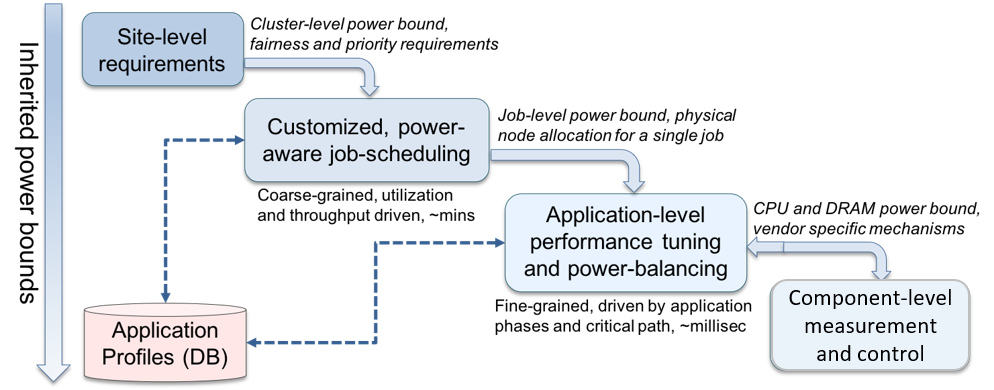
\includegraphics[scale = 0.7]{projects/2.3.1-PMR/2.3.1.19-Argo-PowerSteering/PowerStack_v2.png}
	\caption{Envisioned PowerStack}
	\label{fig:pstack}
\end{figure}

\paragraph{Next Steps}
We will continue our research and development work as planned toward the March 2019 milestones. More specifically, we are migrating to Intel GEOPM's new codebase, working on GPU power capping research, and enabling user-space access to power management on diverse architectures. We also continue to enhance our variation-aware and phase aware model with advanced machine learning and statistical techniques, and are working with Intel on understanding variation data from Theta. In the Legion space, we continue to explore dependency graphs and scheduling of dependency graphs in an intelligent, power-aware manner by creating a new mapper. We are also looking into S3D application code as part of our Legion power model  exploration. Lastly, we are looking into adding Spack support for installing GEOPM. 

\subsubsection{\stid{5.05} Argo} 

\paragraph{Overview} 

The Argo project~\cite{perarnau2017argo} is building portable, open source system software that improves
the performance and scalability and provides increased functionality to
Exascale applications and runtime systems.

We focus on four areas of the OS/R stack where the need from the ECP
applications and facilities is perceived to be the most urgent:
1) support for hierarchical memory;
2) dynamic and hierarchical power management to meet performance
targets;
3) containers for managing resources within a node; and
4) internode interfaces for collectively managing resources across groups
of nodes.


\paragraph{Key Challenges}

Many ECP applications have a complex runtime structure, ranging from in
situ data analysis, through an ensemble of largely independent individual
subjobs, to arbitrarily complex workflow structures~\cite{dreher2017situ}.  At the same time, HPC
hardware complexity increases as well, from deeper memory hierarchies
encompassing on-package DRAM and byte-addressable NVRAM, to heterogeneous
compute resources and performance changing dynamically based on
power/thermal constraints.

To meet the emerging needs of ECP workloads while providing optimal
performance and resilience, the compute, memory, and interconnect resources
must be managed in cooperation with applications and runtime systems; yet
existing resource management solutions lack the necessary capabilities and
vendors are reluctant to innovate in this space in the absence of clear
directions from the community.


\paragraph{Solution Strategy}

Our approach is to augment and optimize for HPC the existing open source
offerings provided by vendors. We are working with ECP applications and
runtime systems to distill the needed new interfaces and to build, test,
and evaluate the newly implemented functionality with ECP workloads.  This
needs to be done in cooperation with facilities, who can provide early
hardware testbeds where the newly implemented functionality can be
demonstrated to show benefits, tested at scale, and matured.  Over the
years we have cultivated an excellent relationship with the vendors
providing HPC platforms because our approach has been to augment and
improve, rather than develop our own OS/R from scratch.  IBM, Cray, and
Intel are eager to integrate the components we develop for ECP that can
help applications.

Our work in each area focuses on the following:

\begin{enumerate}

\item \textbf{Hierarchical memory:} Incorporate NVRAM into the memory hierarchy
using UMap: a user-space \texttt{mmap} replacement for out-of-core data,
leveraging recent \texttt{userfaultfd} mechanism of the Linux kernel for page fault
handling, featuring application-class specific prefetching and eviction
algorithms.  Expose deep DRAM hierarchy by treating high-bandwidth memory
(MCDRAM, HBM) as a scratchpad~\cite{perarnau2016exploring}, managed by the Argonne Memory Library (AML),
which provides applications with asynchronous memory migration
between memory tiers and other convenience mechanisms.

\item \textbf{Power management:}
\emph{PowerStack} explores hierarchical interfaces for power management
at three specific
levels~\cite{Ellsworth:argo,ellsworth_e2sc2016,patki2016,sakamoto2017}: the
global level of batch job schedulers (which we refer to as the Global
Resource Manager or GRM), the enclave level of job-level runtime systems
(open-source solution of Intel GEOPM and the ECP Power Steering project
are being leveraged here), and the node-level through measurement and control
mechanisms integrated with the NRM (described below).
At the node level, we are developing low-level, vendor-neutral
monitoring/controlling capabilities to monitor power/energy consumption,
core temperature and other hardware status~\cite{osti_1353371,zhang2015minimizing}, and control the hardware power
capping and the CPU frequencies. 

\item \textbf{Containers:} Develop a Node Resource Manager (NRM) that leverages
technologies underlying modern container runtimes
(primarily \texttt{cgroups}) to partition resources on compute nodes~\cite{zounmevo2015container},
arbitrating between application components and runtime services.

\item \textbf{Hierarchical resource management:} Develop a set of distributed
services and user-facing interfaces~\cite{perarnau2015distributed} to allow applications and runtimes to
resize, subdivide, and reconfigure their resources inside a job.  Provide
the enclave abstraction: recursive groups of nodes that are managed as a
single entity; those enclaves can then be used to launch new services or to
create subjobs that can communicate with each other.
\end{enumerate}


\paragraph{Recent Progress}

We developed the first stable version of UMap, the user-space memory map
page fault handler for NVRAM.  UMap handler maps application threads'
virtual address ranges to persistent data sets, transparently pages in
active pages and evicts unused pages.  We evaluated the costs and overheads
of various approaches and characterized end-to-end performance for simple
I/O intensive applications.
%
Further work on performance evaluation and capability improvements is
ongoing.  UMap API has been extended to allow for application-specific I/O
strategies.  Read-only support was added to enable the use with released
enterprise versions of the Linux kernel.  UMap now runs on LLNL Sierra.  We
are studying locality-aware eviction and replacement algorithms and are
conducting scaling studies using astronomy application and data.

We developed AML, a memory library for explicit management of deep memory
architectures. Its main feature is a flexible and composable API, allowing
applications to implement algorithms similar to out-of-core for deep
memory.  We provided multiple optimized versions of memory migration
facilities, ranging from a regular copy to a transparent move of memory
pages, using synchronous and asynchronous interfaces and single- and
multithreaded backends.  We validated the initial implementation on Intel's
Knights Landing using a pipelining scheme for stencil applications.  We
also identified interaction points between UMap and AML.  Further
performance and capability improvements are underway.  In particular, we
performed exhaustive studies comparing performance of various approaches
for block-based DGEMM and task-based Cholesky decomposition.

We developed an API between Node Power and Node Resource Manager (NRM),
which in turn allows Global Resource Manager (GRM) to control and monitor
power and other node-local resources.  Additionally, we studied the effect
of power capping on different applications using the NodePower API and
developed power regression models required for a demand-response policy.
We also developed a variation-aware scheduler to address manufacturing
variability under power constraints with Flux infrastructure, and extended
SLURM to support power scheduling plugins.  This was tested on two systems
up to 1,200 nodes and resulted in two publications.  PowerStack is now a
community-wide effort encompassing five industry partners and multiple
academic and research labs across the US, Europe, and Asia.  It enables
prioritization of the critical path, application performance, and
throughput.

We developed the first version of the unified Node Resource Manager.  The
NRM provides high level of control over node resources, including initial
allocation at job launch and dynamic reallocation at the request of the
application and other services.  The initial set of managed resources
includes CPU cores and memory; they can be allocated to application
components via a container abstraction, which is used to describe
partitions of physical resources (to decrease interference), and more.  NRM
integrates dynamic power control using COOLR and libMSR, and provides
support for tracking and reporting of application progress.  Such
functionality is needed by the BSP-oriented power policy, which we are
currently evaluating and scaling up.  Work is also ongoing to support
third-party container technologies such as Docker, Singularity, and
Shifter.  At the job level, we enabled enclave-aware MPI facilities that
can be used to create inter-communicators between MPI jobs launched in
separate enclaves.

On the overall project integration front, we succeeded in creating a first
integrated release, internal for now.  Sources from all the individual
components were pulled into one location.  Testsuites and Spack packages
were created.  We used ChameleonCloud as the first integration platform,
thanks to its capability to provision raw hardware resources.  We also
developed custom CI infrastructure, running on development KNL boxes,
on the ChameleonCloud, and on systems at LLNL.

%\begin{figure}[h]
%\centering
%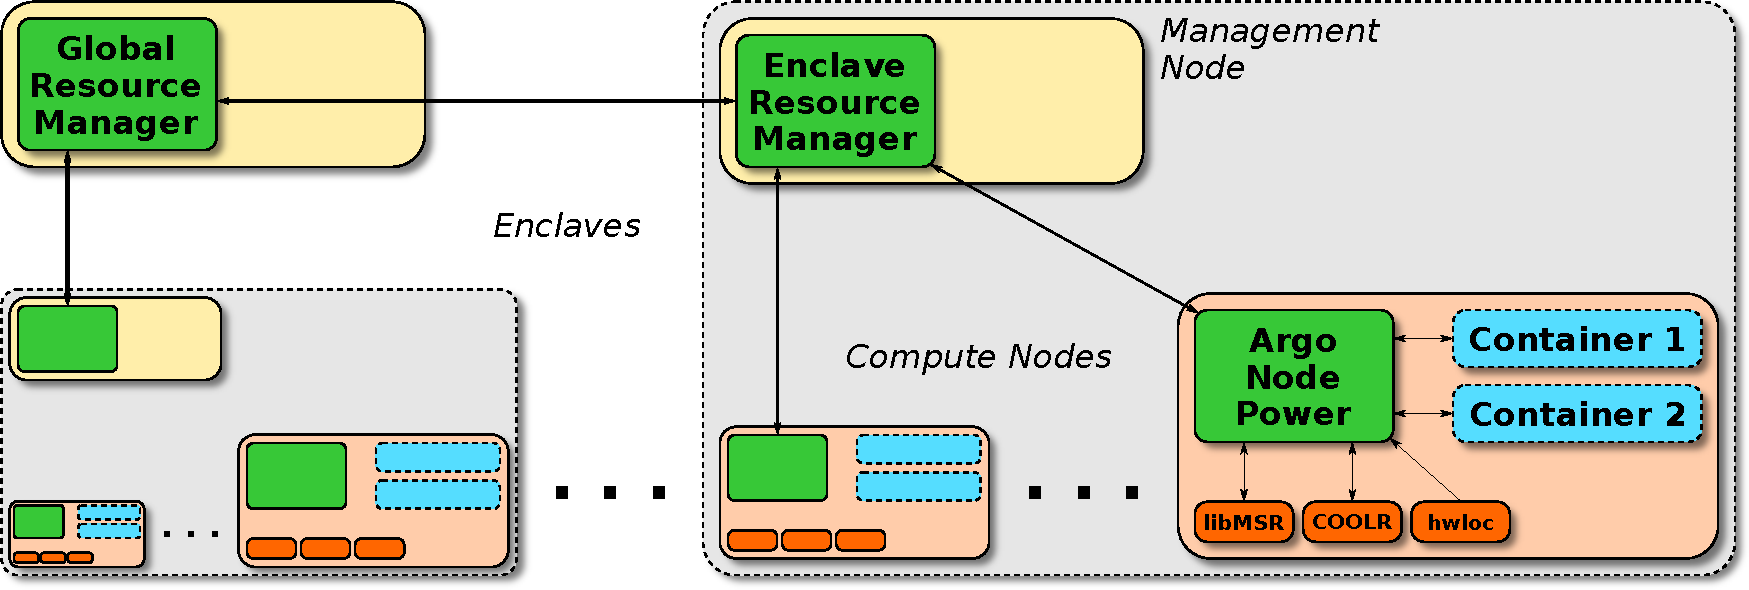
\includegraphics[height=.15\textheight]{projects/2.3.5-Ecosystem/2.3.5.05-Argo/argo-global}\hspace{1em}%
%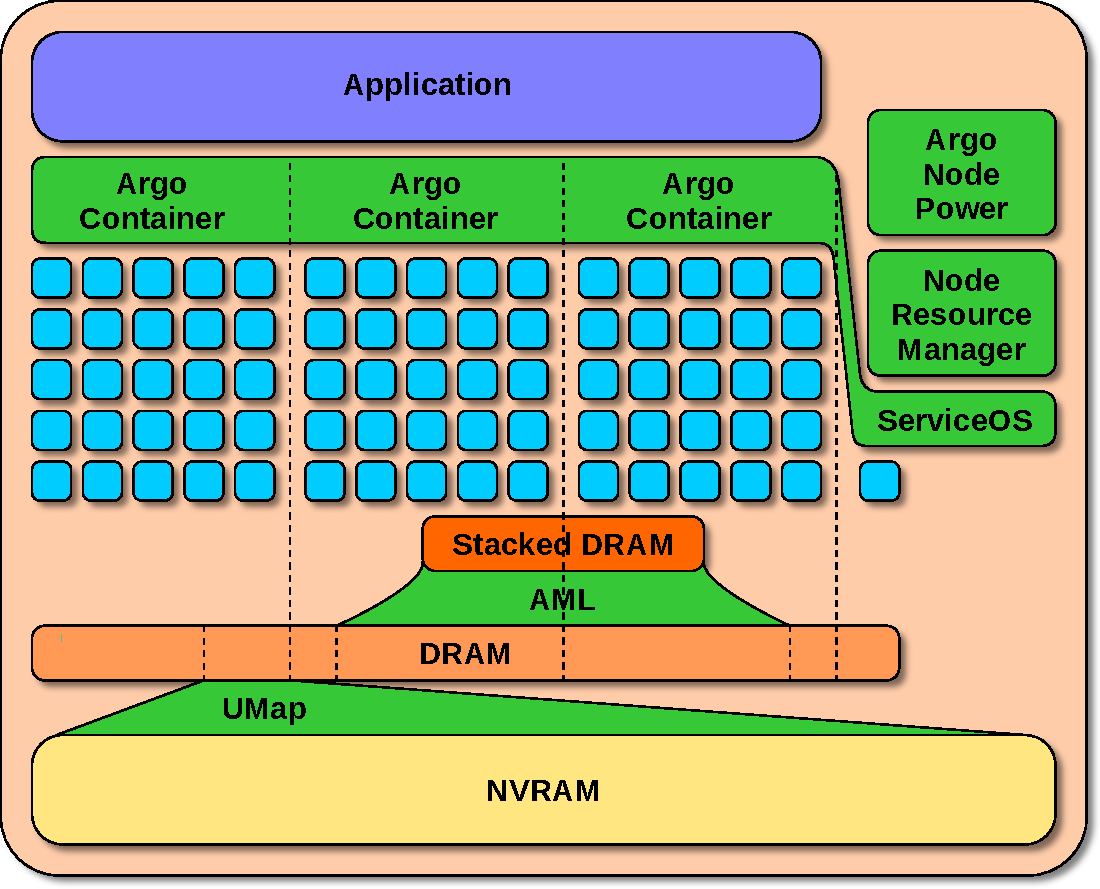
\includegraphics[height=.15\textheight]{projects/2.3.5-Ecosystem/2.3.5.05-Argo/argo-node}
%\caption{Global and node-local components of the Argo software stack and
% interactions between them and the surrounding HPC system components.}
%\end{figure}


\paragraph{Next Steps}

As outlined above, we are actively working on performance and capability
improvements of individual software components and on scaling them up to
leadership-class systems; significant work remains in these areas.

We need to intensify our engagement with ECP applications and runtimes so
that they can benefit from the technologies we have been developing.  We
expect that the newly expanded project team at ANL will enable us to make
significant progress in this area in the near future.

Final software release will take place when the scalability and performance
is validated on a set of relevant ECP workloads.

Looking further into the future, we want to improve resource management for
emerging hardware accelerators, expand dynamic resource management and
placement making it the default, add advanced AI-based autotuning
techniques, use container abstraction to target coupled codes, workflows,
ensembles, and so on.  True byte-addressable NVRAM will enable new,
flexible management and access.

\newpage

\subsection{\tools}
This section present projects in \tools.
\newpage
\subsubsection{\stid{2.01} \tools\ Software Development Kits} 

\paragraph{Overview} 
The \tools\ SDK effort is focused on identifying meaningful aggregations of products in this technical area.  SDK efforts are in the early stages of planning and execution.  Most of the work on SDKs has been driven from the \ecosystem\ technical area.  A description of the SDK effort can be found in Section~\ref{subsubsect:ecosystem-sdk}.

\newpage
\subsubsection{\stid{2.06} Exa-PAPI++}\label{subsubsect:exapapi}

\paragraph{Overview} 

%Understanding the performance characteristics of exascale applications is 
%necessary in order to identify and address the barriers to achieving performance 
%goals. This becomes more difficult as the architectures become more complex. 
%The Performance Application Programming Interface (PAPI) provides both library 
%and application developers with generic and portable access to low-level 
%performance counters found across the exascale machine, enabling users to see
%the relationships between software performance and hardware events. 
%These relationships provide a critical step toward improving performance.

The Exa-PAPI++ 
project is developing a new C++ Performance API (PAPI++) software package 
from the ground up that offers a standard interface and methodology for using
low-level performance counters in CPUs, GPUs, on/off-chip memory, interconnects, 
and the I/O system, including energy/power management. 
PAPI++ is building upon classic-PAPI functionality and strengthening its path to
exascale with a more efficient and flexible software design, one that takes 
advantage of C++'s object-oriented nature but preserves the low-overhead 
monitoring of performance counters and adds a vast testing suite.

In addition to providing hardware counter-based information, a standardizing layer 
for monitoring software-defined events (SDE) is being incorporated that exposes 
the internal behavior of runtime systems and libraries, such as communication and 
math libraries, to the applications. As a result, the notion of performance events is 
broadened from strictly hardware-related events to include software-based 
information. Enabling monitoring of both hardware and software events provides 
more flexibility to developers when capturing performance information.


\paragraph{Key Challenges}

Widely deployed and widely used, PAPI has established itself as fundamental
software infrastructure in every application domain where improving performance
can be mission critical. 
However, processor and system designs have been experiencing radical changes.
Systems now combine multi-core CPUs and accelerators, shared and
distributed memory, PCI-express and other interconnects, and
power efficiency is emerging as a primary design constraint.
These changes pose new challenges and bring new
opportunities to PAPI. At the same time, the ever-increasing importance of
communication and synchronization costs in parallel applications, as well as the
emergence of task-based programming paradigms, pose
challenges to the development of performance-critical applications and create a
need for standardizing performance events that originate from various ECP
software layers.


\paragraph{Solution Strategy}

The Exa-PAPI++ team is preparing PAPI support to stand up to 
the challenges posed by exascale systems by 
\begin{enumerate}
\item widening its applicability and providing robust support for exascale 
hardware resources;
\item supporting finer-grain measurement and control of power, thus offering 
software developers a basic building block for dynamic application optimization 
under power constraints; 
\item extending PAPI to support software-defined events; and 
\item applying semantic analysis to hardware counters so that the application 
developer can better make sense of the ever-growing list of raw hardware 
performance events that can be measured during execution. 
\end{enumerate}

%The Exa-PAPI effort delivers new PAPI components to handle the wide range of
%new hardware and software events for the extreme scale platforms that will form
%the basis of exascale computing. To achieve this, Exa-PAPI implements a variety
%of monitoring and sampling capabilities for the different technologies, which
%are exported to the ECP application community. 
%%
%Exa-PAPI also provides finer-grain measurement and control of power, thus
%offering software developers a basic building block for dynamic application
%optimization under power constraint. Other hardware efforts in Exa-PAPI are the
%development of components for monitoring network interconnect events, as well as
%components targeted at the deep and heterogeneous memory hierarchies that we
%are already seeing in new architectures.

In summary, the team will be channeling the monitoring capabilities of hardware 
counters, power usage, software-defined events into a robust PAPI++ software 
package. PAPI++ is meant to be PAPI's replacement---with a more flexible and 
sustainable software design.


\paragraph{Recent Progress}

On the \textbf{software event} front, the PAPI team has designed and implemented 
a new API to expose any kind of software-defined events. Since September 2019,
the SDE functionality is publicly available through the main repository of PAPI. 
As a result, software packages that reside in any layer of the software stack can now 
export information to the outside world in a uniform, well supported, and 
standardized way. 
 %
Since the concept of software-defined events is still new to PAPI, the team has worked
closely with developers of different ECP libraries and runtimes that serve as natural targets
for the adoption of the new SDE API.
As of today, we have integrated SDEs into the sparse linear algebra library MAGMA-Sparse 
(2.3.3.13 CLOVER), the tensor algebra library TAMM (2.2.1.02 NWChemEx), 
the task-scheduling runtime PaRSEC (2.3.1.09 PaRSEC), and the compiler-based 
performance analysis tool BYFL (2.4.2 HE). 

%\vspace{-4pt}
\begin{figure}[!h]
\begin{center}
  \subfloat[ ]{\label{fig:sde_magma}
  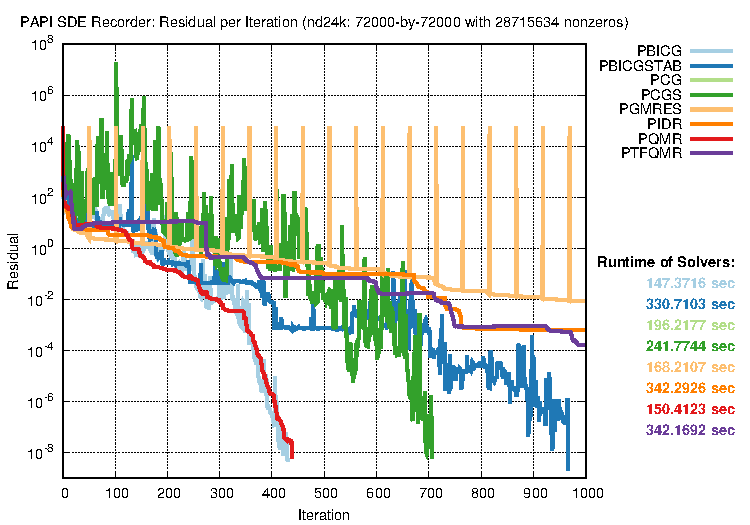
\includegraphics[width=0.49\linewidth]{projects/2.3.2-Tools/2.3.2.06-EXA-PAPI/Exa-PAPI_sde_magma.pdf}}
  \subfloat[ ]{\label{fig:sde_parsec}
  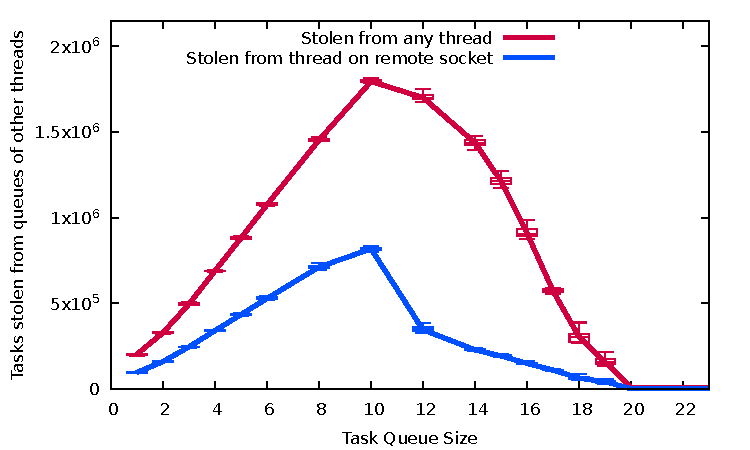
\includegraphics[width=0.49\linewidth]{projects/2.3.2-Tools/2.3.2.06-EXA-PAPI/Exa-PAPI_sde_parsec.pdf}}
%\vspace{-8pt}
\end{center}
\vspace{-9pt}
\caption{(a) PAPI SDE-Recorders log convergence of different ILU-preconditioned MAGMA-sparse Krylov solvers for a 2D/3D Problem; (b) PAPI SDEs count number of times the scheduler stole tasks from the task queue of another thread in PaRSEC.}
\end{figure}
%\vspace{-8pt}
%
%
The examples in Figure~\ref{fig:sde_magma} illustrate how the convergence of Krylov solvers can be
visualized with the help of PAPI SDEs. Each of these solvers behave very differently 
for different problems and matrices, which, once more, stresses the importance of 
\emph{exposing these details in a standardized way}. This allows the domain
scientist to quickly identify the fastest and most robust method of choice for 
their very unique problems. Most importantly, this information can now be obtained without 
expert knowledge about algorithm-specific characteristics,
and without having to instrument MAGMA library code, but simply by calling \verb+PAPI_read()+
in the top-level application.

Figure~\ref{fig:sde_parsec} serves as a second showcase, illustrating the evolution of 
task stealing during the execution of a PaRSEC application that is based on 
fork-join parallelism with 20 tasks generated at each fork.
With SDEs in PARSEC, a user can get a view of what is happening inside the runtime
by simply calling \verb+PAPI_start()+ and \verb+PAPI_stop()+ in their application, without the need to
instrument the PaRSEC runtime code. 


\vspace{10pt}
On the \textbf{hardware counter} front, we have developed support for the latest 
features on NVIDIA Volta GPUs (V100) as featured on the Summit and Sierra systems.
Specifically, PAPI users can now monitor both GPU hardware events and the NVLINK performance. 
Additionally, we developed PAPI capabilities for monitoring power consumption, fan speed, 
temperature, and power capping support for the V100 GPUs. 
The latest version of PAPI (5.7.0, released April 2019) has fully integrated support for the 
NVIDIA GPU counters and power management.
Similar efforts are currently in progress enabling users to monitor performance counters 
as well as power consumption on the AMD Vega GPUs.


\paragraph{Next Steps}

Our next efforts will focus on:
\begin{enumerate}
\item \textbf{Formulation of requirements for new PAPI C++ API:} 
		Create and circulate a survey to the ECP teams to assess their needs for hardware 
		and software performance counter functionality. Based on the survey results, 
		we will determine what features are needed for the new PAPI C++ interface. 
		Furthermore, perform a software requirement analysis, and explore novel concepts 
		for expressing software event and hardware counter 
		monitoring through the same PAPI C++ interface.
%
\item \textbf{Decompose PAPI's SDE functionality as standalone library}: 
		The SDE functionality will be decomposed from the PAPI package and made 
		available as a separate library. The production-ready version of the PAPI SDE 
		library will have fully integrated support for enabling SDEs in ECP software
		layers, as well as monitoring these new events through the PAPI interfaces.
%
\item \textbf{Formulation of a roadmap for refactoring traditional PAPI to PAPI++ software package}:
		Start the PAPI++ design process 
		for a modular framework that includes a new C++ API in addition to the traditional C 
		and Fortran APIs to preserve backward-compatibility. This effort involves a managed 
		transition away from our legacy PAPI software while continuing to add support for new 
		ECP hardware (released during FY20-21) until the official release of PAPI++.
\end{enumerate}

\newpage

\subsubsection{\stid{2.08} HPCToolkit} 
\paragraph{Overview} 

The HPCToolkit project is working to develop performance measurement and analysis tools to help ECP software developers understand where and why their programs do not fully exploit hardware resources within and across nodes of extreme-scale parallel systems. Key deliverables of the project are a suite of software tools that developers need to measure and analyze the performance of parallel applications as they execute on existing ECP testbeds and new technologies needed to measure and analyze performance on forthcoming Exascale systems.

To provide a foundation for performance measurement and analysis, the project team is working with community stakeholders, including standards committees, vendors, and open source developers to improve hardware and software support for measurement and attribution of application performance on extreme-scale parallel systems. The project team has been engaging vendors to improve
 hardware support for performance measurement in next generation systems and working with other software teams to design and integrate new capabilities into operating systems, runtime systems, communication libraries, and application frameworks that will enhance the ability of software tools to accurately measure and attribute code performance on extreme-scale parallel systems.  Using emerging hardware and software interfaces for monitoring code performance, the project team is working to extend capabilities to measure computation, data movement, communication, and I/O as a program executes to pinpoint scalability bottlenecks, evaluate resource consumption, and quantify inefficiencies. 




% HPCToolkit as well as the technologies that the project is contributing to the hardware and software ecosystem is needed for ECP because no existing tools are able to measure and precisely attribute the performance of software executing on scalable parallel systems with heterogeneous node-level compute technologies. The project is working to develop tools that attribute performance of code at all levels of the software stack including the application, runtime systems, libraries, and operating systems on  traditional CPUs as  well as accelerators.

\paragraph{Key  Challenges}

In recent years, the complexity, diversity, and the rate of change of architectures for extreme-scale parallel systems have increased dramatically. For higher efficiency, heterogeneous designs that couple multicore processors with accelerators and employ more complex memory hierarchies have been increasing in importance. In addition,  the DOE is purposefully pursuing multiple independent architectural designs for next generation parallel systems as part of risk mitigation. For performance tools, the need to support multiple diverse architectural paths significantly increases tool complexity. 
% For instance, performance measurement and analysis methodologies for accelerators such as graphics processor units that play a central role in the emerging CORAL systems are completely different than methodologies used for measuring the performance on alternative designs in ECP testbeds based on manycore processors.
At the same time, the complexity of applications is increasing dramatically as developers struggle to expose billion-way parallelism, map computation onto heterogeneous computing elements, and cope with the growing complexity of memory hierarchies. While application developers can employ abstractions to hide some of the complexity of emerging parallel systems, performance tools must be intimately familiar with all of the idiosyncratic features added to these systems to improve performance or efficiency, develop measurement and analysis techniques that assess how well these features are being exploited, and then relate these measurements back to software to create actionable feedback that will guide developers to improve the performance, efficiency, and scalability of their applications.

\paragraph{Solution Strategy}

Development of HPCToolkit as part of ECP is focused on preparing it for production use at Exascale by enhancing it in several ways. First, the team is adding new capabilities to measure and analyze interactions between software and key hardware subsystems in extreme-scale platforms, including more complex memory hierarchies and accelerators. Second, the team is working to improve performance attribution given optimized code for complex node-level programming models used by ECP developers, including OpenMP and template-based programming models such as LLNL's RAJA and Sandia's KOKKOS. To support this effort, the project team is enhancing the Dyninst binary analysis toolkit, which is also used by other ECP tools. Third, the team is improving the scalability of HPCToolkit so that it can be used to measure and analyze extreme-scale executions. Fourth, the project team is working to improve the robustness of the tools across the range of architectures used as ECP platforms. Fifth, the team will enhance HPCToolkit's user interfaces to help analyze performance bottlenecks on extreme-scale platforms.  Finally, the project team will work other ECP teams to ensure that they benefit from HPCToolkit's capabilities to measure, analyze, attribute, and diagnose performance issues on ECP testbeds and forthcoming Exascale systems.  

\paragraph{Recent Progress}

Over the last year, the HPCToolkit project has significantly enhanced the ability to measure and analyze application performance. 

\begin{itemize}
\item
The project team added a new measurement substrate to HPCToolkit to measure performance using the Linux perf\_events interface. Using perf\_events enables HPCToolkit to measure operating system activity and thread blocking in addition to application execution. Figure~\ref{fig:hpctoolkit-kernel} displays a screenshot of HPCToolkit's code-centric user interface that shows how HPCToolkit reports information about kernel activity on behalf of an application as part of an application's performance. 
%The screenshot shows that the performance of data movement occurring as part of interprocess communication in a parallel code is a function of how fast a single hardware thread can perform a copy loop within the operating system kernel.
 \item
To accurately attribute code performance to elements of complex, parallel software frameworks that have been transformed  by optimizing compilers, HPCToolkit employs an approach that combines information recorded by compilers about line maps and the provenance of inlined code with direct analysis of machine code to recover information about a program's control flow. Over the past year, the project team has developed improved techniques for recovering control flow graphs from machine code 
 and employed them to relate application performance to inlined functions, templates, and  loops in highly optimized code on both host processors and attached accelerators. Figure~\ref{fig:hpctoolkit-perfsuite} shows the precise attribution of performance measurements to C++ templates employed as part of LLNL's RAJA portability layer.
\item
The project team has developed novel capabilities for measurement, analysis, and attribution of applications that employ graphics processing units (GPUs) as accelerators.  This work includes leading the design of the OMPT tool application programming interface as part of the emerging OpenMP 5.0 standard, developing a measurement infrastructure as part of {\tt libomptarget}---an open source library for offloading code onto accelerators, enhancing HPCToolkit to ingest measurement data from accelerators, and extending HPCToolkit to analyze binaries for NVIDIA's GPUs to attribute performance of offloaded code. Figure~\ref{fig:hpctoolkit-perfsuite} illustrates how HPCToolkit can attribute the performance of code offloaded onto a GPU to the host context that offloaded the computation.
\end{itemize}

\begin{figure}[t]
\centering
\begin{subfloat}[HPCToolkit kernel activity performance metrics.\label{fig:hpctoolkit-kernel}]%{.48\textwidth}
\centering
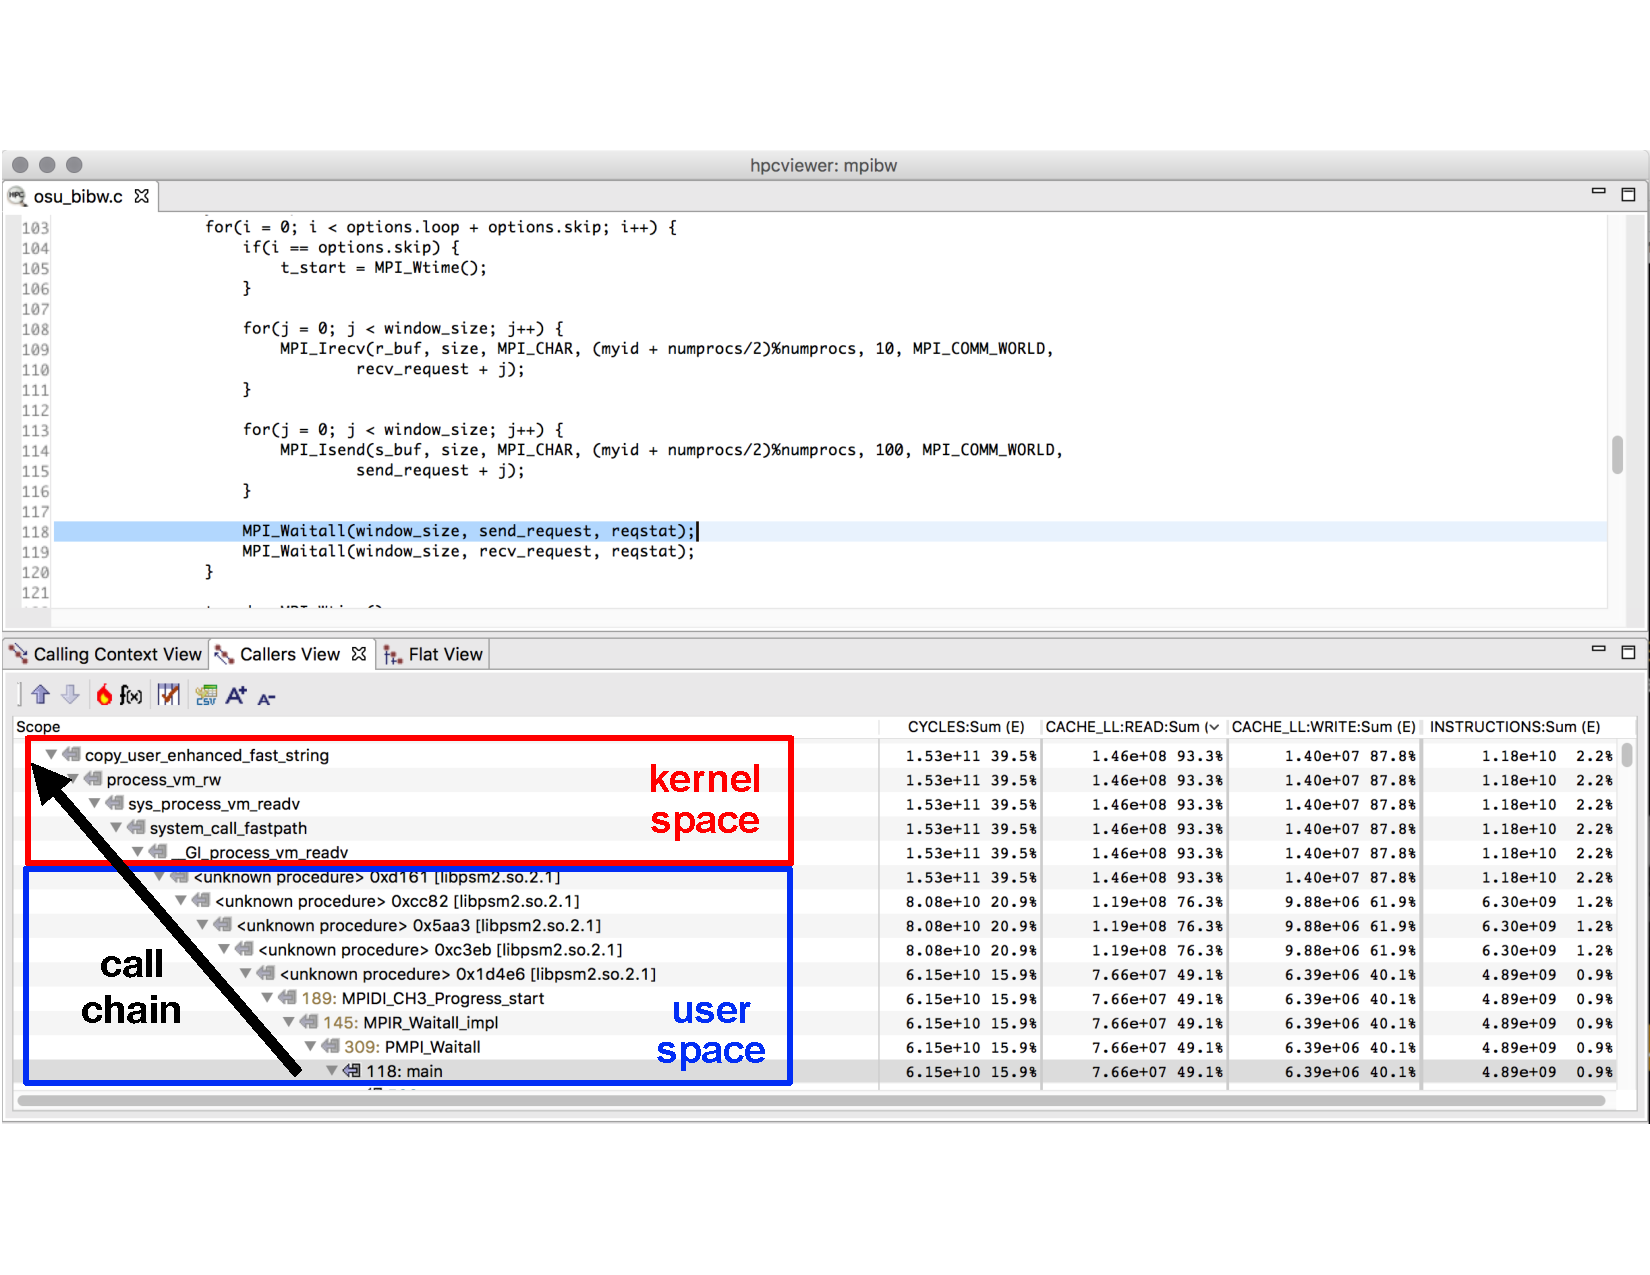
\includegraphics[width=.48\textwidth]{projects/2.3.2-Tools/2.3.2.08-HPCToolkit/hpctoolkit-kernel}
%\caption{The December 2017 release of HPCToolkit includes support for measuring and attributing performance metrics of kernel activity on behalf of an application.}
%\label{fig:hpctoolkit-kernel}
\end{subfloat}
\hfill
\begin{subfloat}[HPCToolkit GPU offloaded performance.
\label{fig:hpctoolkit-perfsuite}]%{.48\textwidth}
\centering
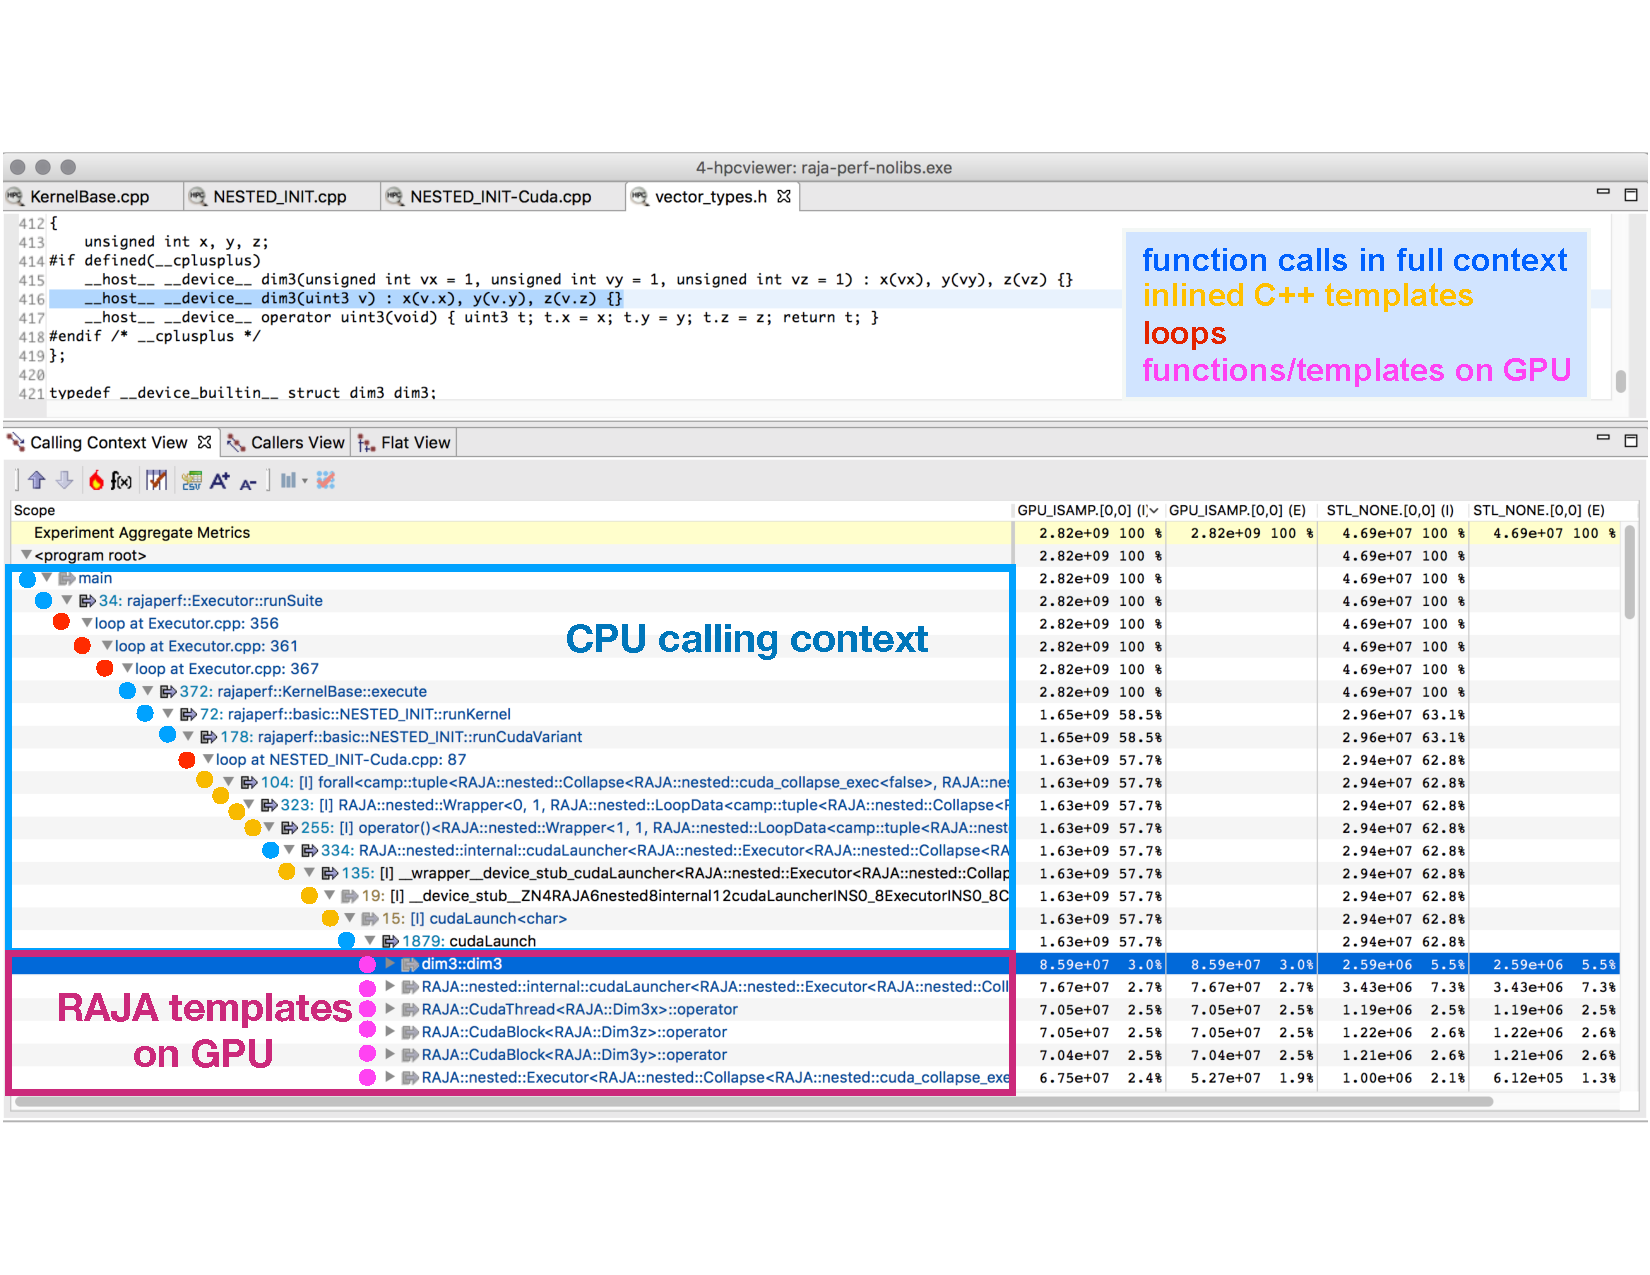
\includegraphics[width=.48\textwidth]{projects/2.3.2-Tools/2.3.2.08-HPCToolkit/hpctoolkit-perfsuite}
%\caption{HPCToolkit now measures and attributes the performance of computation offloaded to GPUs using LLNL's RAJA template-based programming model.}
%\label{fig:hpctoolkit-perfsuite}
\end{subfloat}
\caption{The December 2017 HPCToolkit release supports measuring and attributing performance metrics of kernel activity on behalf of an application.  HPCToolkit now measures and attributes the performance of computation offloaded to GPUs using LLNL's RAJA template-based programming model.}
\end{figure}
\vspace{-1ex}

\paragraph{Next Steps}

The next steps in the project are to:
\begin{itemize}
\setlength\itemsep{0em}
\item Work with the OpenMP standards committee to finalize tool interfaces as part of the emerging OpenMP standard.
\item Complete and deploy implementation of  HPCToolkit's support for measurement and analysis of code offloaded onto NVIDIA GPUs. 
%Work to integrate GPU measurement support back into the open-source {\tt libomptarget} library.
\item Integrate new support for task-based parallelism developed as part of the project's Dyninst binary analysis infrastructure into HPCToolkit's binary analyzer to accelerate analysis of large executables.
\item Complete work on data-centric performance analysis capabilities that  measure and attribute data movement costs to program variables.
\item Complete and deploy a framework for regression testing of HPCToolkit.
\item Work with DOE and Intel on performance measurement technologies for the A21 Exascale platform.
\end{itemize}

\newpage
\subsubsection{\stid{2.10} PROTEAS | Clacc: OpenACC in Clang and LLVM}\label{s:clacc}

\newcommand{\todo}[1]{\textbf{\textcolor{red}{#1}}}

\paragraph{Overview}

Heterogeneous and manycore processors (e.g., multicore CPUs, GPUs, Xeon Phi,
etc.) are becoming the de facto architectures for current HPC platforms and
future Exascale platforms.  These architectures are drastically diverse in
terms of functionality, performance, programmability, and scalability,
significantly increasing the complexity that ECP application developers face
as they attempt to fully utilize the available hardware.

A key enabling technology being pursued as part of the PROTEAS project is
OpenACC.  While OpenMP has historically focused on shared-memory multi-core
programming, OpenACC was launched in 2010 as a portable programming model
for heterogeneous accelerators.  Championed by institutions like NVIDIA,
PGI, and ORNL, OpenACC has evolved into one of the most portable and well
recognized programming models for accelerators today.

Despite the importance of OpenACC, the only non-academic open-source OpenACC
compiler cited by the OpenACC website is GCC \cite{openaccOrgTools}.
However, GCC has lagged behind commercial compilers, such as PGI's, in
providing production-quality support for the latest OpenACC specifications
\cite{openACCValidationSuite}.  Moreover, GCC is known within the compiler
community to be challenging to extend and, especially within the DOE, is
losing favor to clang and LLVM for new compiler research and development
efforts.

\textit{Claac}~\cite{clacc:2018:denny} is a major goal of the PROTEAS project. 
Overall, the goal is to build on clang and LLVM to develop an
open-source, production-quality OpenACC compiler ecosystem that is easily
extensible and that utilizes the latest research in compiler technology.
Such an ecosystem is critical to the successful acceleration of ECP
applications using modern HPC hardware.  
The PROTEAS objectives for clacc are:

\begin{enumerate}

\item Develop production-quality, standard-conforming OpenACC compiler
and runtime support as an extension of clang/LLVM.

\item As part of the compiler design, leverage the clang ecosystem to enable
the future construction of source-level OpenACC tools, such as pretty
printers, analyzers, lint tools, debugger extensions, and editor extensions.

\item As the work matures, contribute OpenACC support to upstream clang/LLVM
so that it can be used by the broader HPC and parallel programming
communities.

\item Throughout development, actively contribute upstream any clang/LLVM
improvements that are mutually beneficial to both our OpenACC work and to
the broader clang/LLVM ecosystem.

% \item OpenARC is our in-house compiler for OpenACC.  We are utilizing
% OpenARC as a research platform for rapidly prototyping cutting-edge compiler
% techniques for translating and optimizing OpenACC.

\end{enumerate}

%\todo{Talk about our experience with OpenARC and how that positions us well
%to work on OpenACC?}

\paragraph{Key Challenges}

\begin{enumerate}

\item \textbf{OpenACC Support:} Developing production-quality,
standards-conforming OpenACC compiler and runtime support is a large
undertaking.  Complicating that undertaking further is the need for
optimization strategies that are competitive with existing commercial
compilers, such as PGI's, which have been developed over many years since
before the conception of the OpenACC standard.

\item \textbf{Source-to-Source:} Source-to-source translation from OpenACC
to another programming language can significantly reduce the effort to
implement OpenACC.  However, a well known issue with LLVM's compiler front
end, clang, is that its AST, the source-level representation, was designed
to be immutable.  Moreover, analysis and optimization capabilities are
implemented at the level of the LLVM intermediate representation (IR) not at
the AST level, but such capabilities would be critical for lowering
OpenACC's descriptive language to a more prescriptive language, like OpenMP.

\item \textbf{Production-Quality:} Clang and LLVM are sophisticated tools
with a complex codebase and a large team of developers who diligently screen
contributions to maintain a clean design and correct operation.  As for any
production-quality compiler, developing and contributing improvements to
clang and LLVM can be significantly more challenging and time-consuming than
for research-quality compilers.

\item \textbf{OpenMP Alternative:} We believe that OpenACC's current
momentum as the go-to directive-based language for accelerators will
continue into the foreseeable future.  Nevertheless, some potential OpenACC
adopters hesitate over concerns that OpenACC will one day be replaced by
OpenMP features.  A tool to migrate OpenACC applications to OpenMP could
alleviate such concerns, encourage adoption of OpenACC, and thus advance
utilization of acceleration hardware in ECP applications.

\end{enumerate}

\paragraph{Solution Strategy}

~
\vspace{-1em}

\begin{tabular}{@{\hspace{-1.5em}}p{.77\textwidth}p{.23\textwidth}@{}}

\begin{enumerate}

\item A key feature of the clacc design is to lower OpenACC to OpenMP.  This
design has several benefits:

\begin{enumerate}

\item By building on clang/LLVM's existing OpenMP compiler and runtime
support, it reduces the effort necessary to construct a production-quality
OpenACC implementation.

\item It facilitates repurposing for OpenACC existing OpenMP static analysis
and debugging tools.

\item It facilitates porting applications from OpenACC to OpenMP to
alleviate the aforementioned concerns about developing applications in
OpenACC.

\end{enumerate}

\item To ensure clacc's successful implementation and eventual acceptance
upstream, we have begun and will continue design discussions with the
clang/LLVM communities throughout clacc's development.

\item To handle clang's immutable AST, clacc's design reuses a clang feature
called TreeTransform, which was originally designed for C++ template
specializations.

\end{enumerate}

&

\raisebox{-\totalheight}{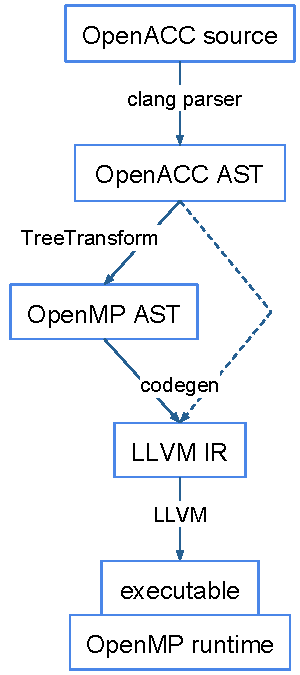
\includegraphics[scale=.65]{projects/2.3.2-Tools/2.3.2.10-PROTEAS-YTUNE/clacc.pdf}}

\end{tabular}

\vspace{-1em}

\begin{enumerate}

\setcounter{enumi}{3}

\item To take advantage of analyses and optimizations at the LLVM IR level,
we are investigating ongoing efforts to develop a parallel LLVM IR, which
clacc could use as an alternative code generation target.

\item To stage our development effort, we are initially implementing clacc
with two simplifications: we are implementing a prescriptive interpretation
of OpenACC to achieve correct behavior, and we are implementing and testing
only within C.  We will extend this implementation with the necessary
analyses and optimizations for a descriptive interpretation and for C++
afterward.  

\item Throughout clacc development, we are continuously integrating the
latest upstream clang/LLVM changes, and we are running and extending the
clang/LLVM test suites to detect regressions and incompatibilities.  We are
also investigating OpenACC benchmarks \cite{specAccel} and validation test
suites \cite{openACCValidationSuite} to ensure correct OpenACC behavior and
good performance.

% \item We will utilize OpenARC, an OpenACC compiler we have developed
% in-house as a research platform for rapidly prototyping cutting-edge
% compiler analyses and optimizations.  After a successful proof-of-concept
% implementation in OpenARC, we will port and harden such compiler techniques
% in clacc.

\end{enumerate}


\paragraph{Recent Progress}

\begin{enumerate}

\item Prototyped the translation of an initial set of OpenACC directives and
clauses to OpenMP.

\item Investigated OpenACC applications, benchmarks, and validation test
suites for use in clacc testing.  Reached out to ECP application teams who
have expressed interest in OpenACC.

\item Initiated clacc design discussions within the clang/LLVM developer
community.

\item Contributed to upstream clang/LLVM a number of fixes and other
improvements to clang attribute and printing support, the clang/LLVM testing
infrastructure, and the OpenMP implementation.

\end{enumerate}


\paragraph{Next Steps}

\begin{enumerate}

\item Complete clacc support for a prescriptive interpretation of OpenACC
for correct behavior, and continue to contribute mutually beneficial
improvements to upstream clang/LLVM as we develop them.

\item Continue clacc design discussions with the clang/LLVM developer
community.

\item Explore applications from ECP teams we have previously contacted.
	
\end{enumerate}

\subsubsection{\stid{2.10} PROTEAS | PAPYRUS: Parallel Aggregate Persistent Storage}\label{s:papyrus}

\paragraph{Overview} 
Papyrus is a programming system that provides features for scalable, aggregate, persistent memory in an extreme-scale system for typical HPC usage scenarios. Papyrus provides a portable and scalable programming interface to access and manage parallel data structures on the distributed NVM storage. Papyrus allows the programmers to exploit large aggregate NVM space in the system without handling complex communication, synchronization, replication, and consistency models. Papyrus consists of three components, virtual file system (VFS)~\cite{Kim:2017:DIP}, C++ template container library (TCL)~\cite{Kim:2017:DIP}, and key-value store (KV)~\cite{Kim:2017:PHP}.
%Figure~\ref{fig:papyrus-fig} illustrates the overview of Papyrus.
(1) PapyrusVFS provides a uniform aggregate NVM storage image for the different types of NVM architectures. It presents an illusion of a single large NVM storage for all NVM devices available in the distributed system. Unlike other traditional kernel-level VFSs, PapyrusVFS is a lightweight user-level VFS, which is provided as a library so that applications can link to or dynamically load it. PapyrusVFS implements a subset of POSIX API related to file I/O. (2) PapyrusTCL provides a high-level container programming interface whose data elements can be distributed to multiple NVM nodes. PapyrusTCL provides three containers, including map, vector, and matrix, implemented as C++ templates. PapyrusTCL is built on top of PapyrusVFS. This enables PapyrusTCL to be decoupled from a specific NVM architecture and to present a high-level programming interface whose data elements are distributed across multiple NVM nodes transparently. (3) PapyrusKV is a novel embedded KVS implemented specifically for HPC architectures and applications to provide scalability, replication, consistency, and high performance, and so that they can be customized by the application. It stores keys and values in arbitrary byte arrays across multiple NVMs. PapyrusKV provides configurable consistency technique controlled by the application during the program execution dynamically to meet application-specific requirements and/or needs. It also supports fault tolerance and streamlined workflow by leveraging NVM's persistence property.

%\begin{figure}[htb]
%    \centering
%    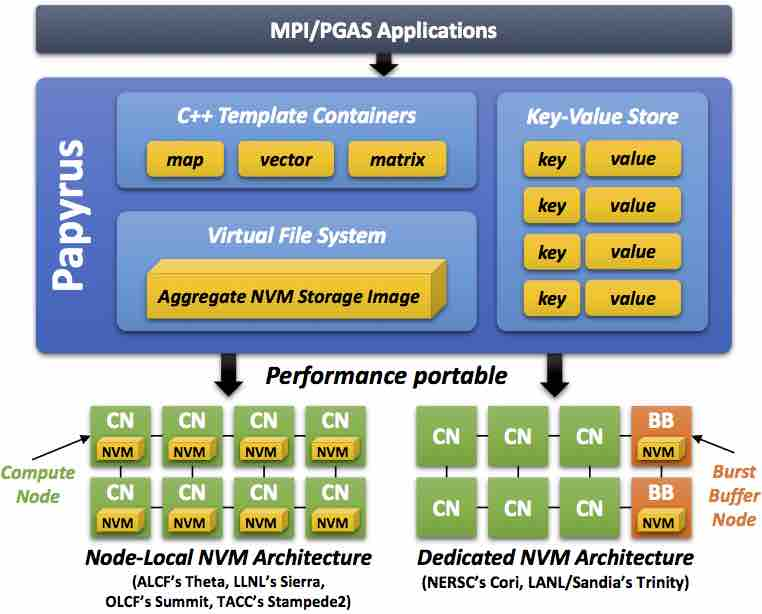
\includegraphics[width=5in]{papyrus-fig}
%    \caption{\label{fig:papyrus-fig}Papyrus consists of three components, virtual file system, C++ template containers, and key-value store}
%\end{figure}

\paragraph{Key Challenges}
In HPC, NVM is quickly becoming a necessary component of future systems, driven, in part, by the projections of very limited DRAM main memory per node and plateauing I/O bandwidth. More concretely, recently-announced DOE systems, such as NERSC's Cori, LANL/Sandia's Trinity, LLNL's Sierra, OLCF's Summit, TACC's Stampede2, and ALCF's Theta, include some form of NVM. This NVM will be used in two fundamental ways. First, it will be used as a cache for I/O to and from the traditional HDD-based external parallel file systems. In this case, most scientists believe that the caching can be implemented transparently, shielding complexity from the applications and users. Second, NVM will be used as an extended memory to provide applications with access to vast amounts of memory capacity beyond what is feasible with DRAM main memory. More interestingly, in HPC, this extended memory can be aggregated into a much larger, scalable memory space than that provided by a single node alone. In this second case, however, no portable and scalable programming systems exist.

\paragraph{Solution Strategy}
We describe our key goals for Papyrus: high performance, scalability, portability, interoperability with existing programming models, and application customizability. First, \textbf{high performance} is a clear need in HPC. The design of Papyrus should provide the opportunity to exploit NVM resources efficiently. Second, \textbf{scalability} is important in HPC as most of the applications must run on large sectors of the systems - thousands to hundreds of thousands of processors. Papyrus should not inhibit scalability; it should provide an interface that is able to scale as the application and system do. Third, \textbf{portability} is a necessary requirement because HPC applications must be able to run on multiple, diverse platforms at any given time. The upcoming DOE systems all have NVM integrated into the systems in different ways. Papyrus must provide both functional portability and performance portability across systems with different architectures. Fourth, \textbf{interoperability} is a practical requirement of HPC applications. Papyrus must be designed so that it can be incrementally introduced into an application without conflicting with existing HPC programming models and languages like MPI, UPC, OpenMP, OpenACC, C, C++, and Fortran. Furthermore, Papyrus should leverage characteristics of these other programming models when possible. Interoperability allows programmers to adopt Papyrus incrementally in legacy MPI applications avoiding major rewrites of the application. Fifth, \textbf{application customizability} is a key requirement to achieve high performance and scalability. HPC applications have many different usage scenarios, and thus Papyrus should have customizable parameters for key features that impact other important properties like performance and scalability.

\paragraph{Recent Progress}

Meraculous~\cite{Georganas:2014:PDB} is a state-of-the-art de novo assembler written in UPC. Its parallel algorithm for de Bruijn graph construction and traversal leverages the one-sided communication in UPC to facilitate the requisite random access pattern in the global de Bruijn graph. The de Bruijn graph is implemented as a distributed hash table with an overlapping substring of length {\it k}, referred to as a {\it k-mer}, as key and a two-letter code [ACGT][ACGT] as value as shown in \autoref{fig:papyrus-meraculous}. A hash function is used to define the affinities between UPC threads and hash table entries. We ported the distributed hash table written in UPC to a PapyrusKV database. The keys in the database are k-mers and the values are two-letter codes. The PapyrusKV runtime calls the same hash function in the UPC application to determine the owners of key-value pairs in the database by specifying the custom hash function when the database is created. Thus, the thread-data affinities in UPC and PapyrusKV are the same as shown in \autoref{fig:papyrus-meraculous}. PapyrusKV requires fewer lines of source code than UPC because it calls standard put and get API functions without implementing an application-specific algorithm for the distributed hash table construction and traversal. \autoref{fig:papyrus-meraculous-eval} shows the performance comparison between PapyrusKV and UPC of Meraculous on Cori. Both versions are built and run using Berkeley UPC, an MPI-interoperable UPC implementation. We measured the total execution time on 32, 64, 128, 256, and 512 UPC threads (32 UPC threads per node). UPC shows better performance than PapyrusKV due to its RDMA capability and built-in remote atomic operations during the graph traversal. The performance gap between UPC and PapyrusKV decreases as the number of UPC threads increases. On 512 UPC threads, PapyrusKV runs 1.5 times slower than UPC. This is mainly because of the asynchronous migration in PapyrusKV during the graph construction.

%\begin{figure}[htb]
%\centering
%\includegraphics[width=3in]{projects/2.3.2-Tools/2.3.2.09-PROTEAS/papyrus-meraculous}
%\caption{K-mer distributed hash table implementations in UPC and PapyrusKV.}
%\label{fig:papyrus-meraculous}
%\end{figure}
%
%\begin{figure}[htb]
%\centering
%\includegraphics[width=3in]{projects/2.3.2-Tools/2.3.2.09-PROTEAS/papyrus-meraculous-eval}
%\caption{Meraculous performance comparison between PapyrusKV (PKV) and UPC on Cori.}
%\label{fig:papyrus-meraculous-eval}
%\end{figure}


\begin{figure}[t]
    \centering
    \begin{subfloat}[K-mer distributed hash table implementations in UPC and PapyrusKV.\label{fig:papyrus-meraculous}]
        \centering
        \includegraphics[width=.48\textwidth]{projects/2.3.2-Tools/2.3.2.10-PROTEAS-YTUNE/papyrus-meraculous}
    \end{subfloat}
    \hfill
    \begin{subfloat}[Meraculous performance comparison between PapyrusKV (PKV) and UPC on Cori.\label{fig:papyrus-meraculous-eval}]
        \centering
        \includegraphics[width=.48\textwidth]{projects/2.3.2-Tools/2.3.2.10-PROTEAS-YTUNE/papyrus-meraculous-eval}
    \end{subfloat}
    \caption{Using PapyrusKV for Meraculous.}
\end{figure}

%\begin{figure}[t]
%    \centering
%    \begin{subfigure}[b]{0.45\textwidth}
%        \includegraphics[width=.99\textwidth]{projects/2.3.2-Tools/2.3.2.09-PROTEAS/papyrus-meraculous}
%        \caption{K-mer distributed hash table implementations in UPC and PapyrusKV.}
%        \label{fig:papyrus-meraculous}        
%    \end{subfigure}
%    \hfill
%    \begin{subfigure}[b]{0.45\textwidth}
%        \includegraphics[width=.99\textwidth]{projects/2.3.2-Tools/2.3.2.09-PROTEAS/papyrus-meraculous-eval}
%        \caption{Meraculous performance comparison between PapyrusKV (PKV) and UPC on Cori.}
%        \label{fig:papyrus-meraculous-eval}
%    \end{subfigure}
%    \caption{Using PapyrusKV for Meraculous.}
%\end{figure}


This past year, we have added data compression and encryption to Papyrus. For data compression, the overhead of data access and movement becomes a serious bottleneck compared to compute overhead in large-scale HPC systems. We integrated data compression methods into Papyrus to achieve storage reduction and performance improvement. 
For data encryption, we need to protect sensitive data (e.g., health records, DNA data) that is being used in distributed infrastructures, and users need practical methods to secure their data throughout its lifecycle. We will introduce data encryption in Papyrus to add an extra layer of security in the complex scientific workflows.


\paragraph{Next Steps}
Our next efforts are:

\begin{enumerate}
\item \textbf{Versioning: } Versioning can be used to provide new levels of reliability and performance optimization. We will design and implement versioning in Papyrus.

\item \textbf{Performance optimization:} New APIs and hardware support is being developed for NVM technologies; we are implementing optimizations in Papyrus to take advantage of these advances.

\end{enumerate}

\subsubsection{\stid{2.10} PROTEAS-TUNE: Programming Toolchain for Emerging Architectures and Systems} 

\paragraph{Key  Challenges:}
Programmer productivity and performance portability are two of the most important challenges facing users of future exascale computing platforms. Application developers targeting ECP architectures will find it increasingly difficult to meet these two challenges without integrated capabilities that allow for flexibility, composability, and interoperability across a mixture of programming, runtime, and architectural components. 

\paragraph{Solution Strategy:}
The PROTEAS-TUNE project was formed as a strategic response to this challenge. (The PROTEAS-TUNE project is the result of the merging of previous ECP projects PROTEAS [PROgramming Toolchain for Emerging Architectures and Systems] and Y-Tune: Autotuning for Cross-Architecture Optimization and Code Generation in FY20.) 
This project has three high-level goals. First, PROTEAS-TUNE will provide a programming pathway to anticipated exascale architectures by addressing programmability and portability concerns of emerging technology trends seen in emerging architectures. In particular, the project focuses on improvements to LLVM and OpenACC. Additionally, the team has significant experience with CUDA, OpenCL, and other programming models that will enable ECP applications teams to explore programming options to find the most effective and productive approaches without constraining programming models or software solutions. Second, PROTEAS-TUNE will prototype an integrated programming framework strategy will deliver solutions on these emerging architectures that will be further refined for these architectural capabilities, and make sure that they transition to vendors, standards activities, applications, and facilities. Thirdly, PROTEAS-TUNE includes autotuning which makes it possible to separate a high-level C/C++/FORTRAN implementation from architecture-specific implementation (OpenMP, OpenACC, CUDA, etc.), optimization, and tuning. It also provides a flexible programming framework and integrated toolchain that will provide ECP applications the opportunity to work with programming abstractions and to evaluate solutions that address the exascale programming challenges they face. 


Specifically, the PROTEAS-TUNE focuses on seven thrusts to improve capabilities and performance portability for applications on exascale architectures: 

\begin{itemize}
\item 
    Improve the core-LLVM compiler ecosystem; 
\item 
	Design and implement the OpenACC heterogeneous programming model for LLVM (Clacc);
\item 
	Use performance modeling and optimization to enable code transformation and performance portability;
\item 
	Refine autotuning for OpenMP and OpenACC programming models in order to directly target challenges with heterogeneous architectures;
\item 
    Improve performance measurement and analysis tools (TAU) for the target exascale architectures and apply it to applications to improve performance;
\item 
    Develop and implement portable software abstractions (Papyrus) for managing persistent memory; and,
\item 
    Aggressively engage applications, SDK, vendor, and software teams to demonstrate and deploy.
    
\end{itemize}

Importantly, the team’s solutions are based on significant, continuing work with LLVM, OpenACC, OpenMP, ARES HLIR, OpenARC, TAU, SuRF and CHiLL. The team has extensive experience and a demonstrated track record of accomplishment in all aspects of this proposed work including existing software deployments, interaction with application teams, vendor interaction, and participation in open source community and standards organizations. Also, the team champions its successful solutions in ECP procurements, community standards, and open-source software stacks, like LLVM, in order to improve their use.

%\paragraph{Key  Challenges:}
%Programmer productivity and performance portability are two of the most important challenges facing applications targeting future Exascale computing platforms. Application developers targeting evolving ECP architectures will find it increasingly difficult to meet these dual challenges without help from integrated capabilities that allow for flexibility, composability, and interoperability across a mixture of programming, runtime, and architectural components. In particular, an integrated programming toolchain is critical for Exascale delivery. First, it will provide a programming pathway to anticipated Exascale architectures by addressing programmability and portability concerns of emerging technology trends seen in pre-procurement machines. It will also enable ECP applications teams to explore programming options to find the most effective and productive approaches without constraining programming models or software solutions. Second, an integrated programming framework strategy will deliver solutions that will be further refined for the architecture capabilities known to be in the system procurement. This is essential for maintaining developer productivity and attaining performance portability as ECP requirements evolve.
%
%
%\paragraph{Solution Strategy:}
%The PROTEAS (\textit{PROgramming Toolchain for Emerging Architectures and Systems}) project is a strategic response to the continuous changes in architectures and hardware that are defining the landscape for emerging ECP systems. PROTEAS is a flexible programming framework and integrated toolchain that will provide ECP applications the opportunity to work with programming abstractions and to evaluate solutions that address the Exascale programming challenges they face. Specifically, the PROTEAS objectives are to
%
%\begin{enumerate}
%    
%    \item Provide productive and performance-portable programming solutions based on directive-based methodologies that support current language paradigms and flexible prototyping of interfaces specifically directed at heterogeneous and manycore processors, deep memory hierarchies, and nonvolatile memory systems (NVM);
%    
%    \item Provide integrated performance assessment solutions for these programming systems that will enable automatic performance analysis and performance-driven optimization;
%    
%    \item Provide an integrated programming toolchain that is powerful enough to prototype the above solutions, while flexible enough to extend its functionality over time;
%    
%    \item Refine our toolchain and solutions through engagement with ECP applications teams who will evaluate prototypes, provide feedback, promote application readiness, and facilitate use of ECP prototype and eventual production machines; and,
%    
%    \item Champion our successful solutions in ECP procurements, community standards (e.g., OpenACC, OpenMP), and open-source software stacks (e.g., LLVM).
%    
%\end{enumerate}
%
%Our team has started with a strong existing base of relevant technological and software capabilities. Importantly, our solutions are based on our significant, continuing work with LLVM, ARES HLIR, OpenARC, and TAU. We have extensive experience and a demonstrated track record of accomplishment in all aspects of this proposed work including existing software deployments, interaction with application teams, vendor interaction, and participation in open source community and standards organizations.
%
%Our strong emphasis on delivering an effective toolchain to application developers within the next few years emphasizes the importance of adopting an integrated programming solution that will be further refined for the architecture capabilities known to be in the Exascale system procurement. We will develop an integrated system (i.e. compilers, runtime systems, debuggers, and performance tools) suitable for deployment in the 2021 timeframe. The experience gained from this development will inform vendor collaborations, proposals to standards committees, and existing open source software to make key elements of our developed technology ready for ECP deployment, either from vendors, through the ECP SDKs, or directly from other open-source venues.
%
%While PROTEAS will be oriented towards foreseeable architectural trends, it will not lock in to specific choices that will constrain what new hardware features it can address. Rather, it is important for the programming framework to embody interoperability, open interfaces, and flexibility in the toolchain, allowing it to pursue high-value solutions as opportunities arise and thereby achieve Exascale performance potential. 

\paragraph{Recent Progress:}

Our recent work has focused on five topics:

\begin{enumerate}
    
    \item OpenACC and Clacc~\cite{clacc:2018:denny}. Develop production-quality, standard-conforming OpenACC compiler and runtime support as an extension of Clang/LLVM. See \S\ref{s:clacc}.
    
    \item Papyrus~\cite{Kim:2017:DIP,Kim:2017:PHP} for portability across NVM architectures. 
    Develop a portable interface to NVM architectures to provide massive, persistent data structures as required by many applications.
    See \S\ref{s:papyrus}.
    
    \item Performance analysis with Tau by adding additional functionality for new architectures. 
    Improve a widely-used performance analysis framework by adding functionality for new architectures and software systems.
    See \S\ref{subsubsect:tau}.

    \item Improving LLVM. In collaboration with numerous other ECP projects, PROTEAS is contributing improvements to the LLVM compiler infrastructure. These improvements include simple bugfixes to the existing infrastructure, monitoring Flang progress, developing Clacc (see \S\ref{s:clacc}), and contributing to the development of a new parallel intermediate representation (see \url{https://github.com/Parallel-IR/llvm-pir/wiki}).
    
    \item Outreach and collaboration with ECP applications teams. 
    We have interacted with over a dozen applications teams to help prepare their applications for ECP. See \S\ref{s:clacc}, \S\ref{s:papyrus}, and \S\ref{subsubsect:tau}.
    
\end{enumerate}

\paragraph{Next Steps:}

Our next efforts are:

\begin{enumerate}
	\item Clacc. Continue developing OpenACC support by lowering OpenACC directives to use the existing LLVM OpenMP infrastructure.
    
	\item Papyrus. Improve support for versioning and other performance improvements.
    
    \item Tau. Improve performance instrumentation for deep memory hierarchies in Tau, focusing primarily on various GPUs and emerging NVM.
    
    \item LLVM Parallel IR. Develop a conceptual prototype for mapping LLVM Clang operations to the proposed Parallel IR, and implement a prototype.

\end{enumerate}

\subsubsection{\stid{2.10} PROTEAS | TAU Performance System}\label{subsubsect:tau}

\paragraph{Overview} 
The TAU Performance System is a versatile profiling and tracing toolkit that supports performance instrumentation, measurement, and analysis. It is a robust, portable, and scalable performance tool for use in parallel programs and systems over several technology generations. It is a ubiquitous performance tool suite for shared-memory and message-passing parallel applications written in C++, C, Fortran, Java, Python, UPC, and Chapel. In the PROTEAS project, TAU is being extended to support compiler-based instrumentation for the LLVM C, C++, and Fortran compilers using higher-level intermediate language representation. TAU is also targeting support for performance evaluation of directive based compilation solutions using OpenARC and it will support comprehensive performance evaluation of NVM based HPC systems.  Through these and other efforts, our objective to better support parallel runtime systems such as OpenMP, OpenACC, Kokkos, ROCm, and CUDA in TAU. Figure~\ref{figure:tau} gives an example of using TAU's parallel profile analysis tool, ParaProf.

\paragraph{Key Challenges} 
Scalable Heterogeneous Computing (SHC) platforms are gaining popularity, but it is becoming more and more complex to program these systems effectively and to evaluate their performance at scale. Performance engineering of applications must take into account multi-layered language and runtime systems, while mapping low-level actions to high-level programming abstractions.  Runtime systems such as Kokkos can shield the complexities of programming SHC systems from the programmers, but pose challenges to performance evaluation tools.  Better integration of performance technology is required.  Exposing parallelism to compilers using higher level constructs in the intermediate language provides additional opportunities for instrumentation and mapping of performance data.  It also makes possible developing new capabilities for observing multiple layers of memory hierarchy and I/O subsystems, especially for NVM-based HPC systems. 

\paragraph{Solution Strategy} Compilers and runtime systems can expose several opportunities for performance instrumentation tools such as TAU.  For instance, using the OpenACC profiling interface, TAU can tap into a wealth of information during kernel execution on accelerators as well measure data transfers between the host and devices. This can highlight when and where these data transfers occur and how long they last.  By implementing compiler-based instrumentation of LLVM compilers with TAU, it is possible to how the precise exclusive and inclusive duration of routines for programs written in C, C++, and Fortran.  Furthermore, we an take advantage of the Kokkos profiling interface to help map lower level performance data to higher level Kokkos constructs that are relevant to programmers. The instrumentation at the runtime system level can be achieved by transparently injecting the TAU Dynamic Shared Object (DSO) in the address space of the executing application. This requires no modification to the application source code or the executable. 

\begin{figure}[htb]
\centering
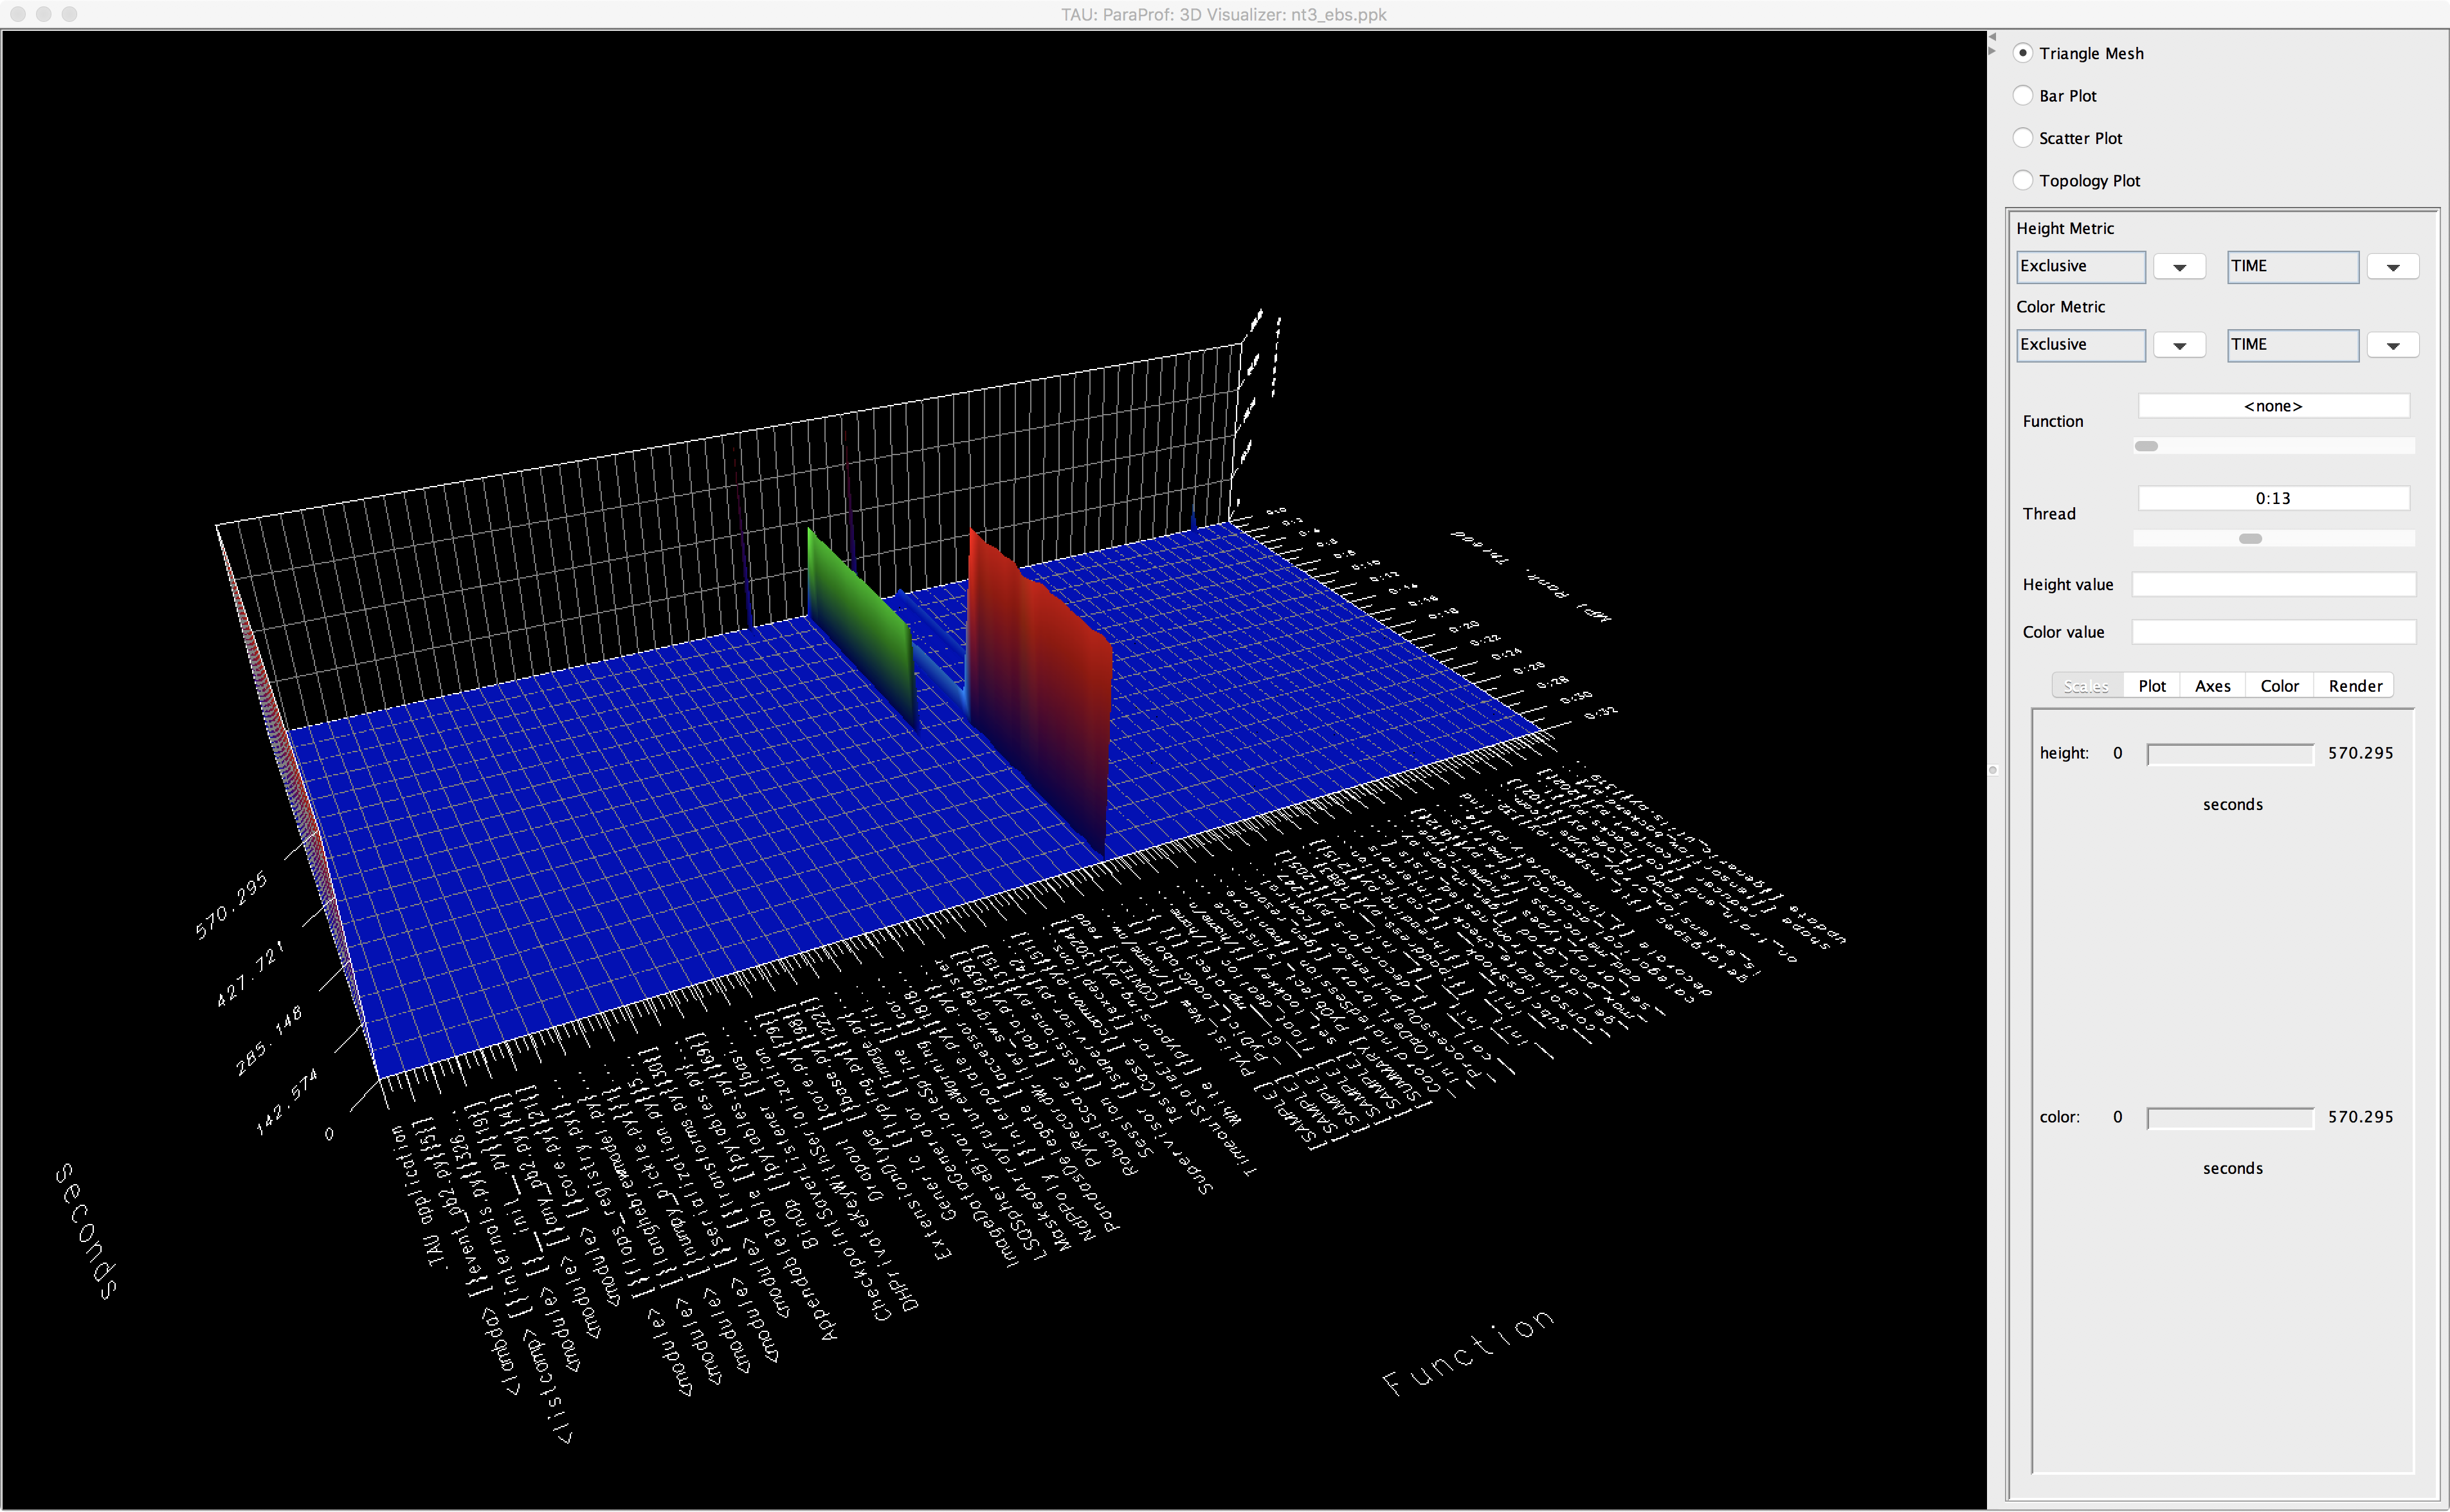
\includegraphics[width=6in]{projects/2.3.2-Tools/2.3.2.10-PROTEAS-YTUNE/tau-3d-candle}
\caption{
  TAU's ParaProf profile browser shows the parallel performance of the CANDLE application, where half the threads are engaged in one activity (\texttt{pthread\_cond\_wait}) while the other half is engaged in some other activity (\texttt{Eigen::internal::gebp\_kernel}).
}
\label{figure:tau}
\end{figure}

\paragraph{Recent Progress}
\begin{enumerate}
\item \textbf{CANDLE} Extended TAU to enhance performance evaluation of multii-threaded Python3 and CUDA and applied it to evaluate the performance of the CANDLE ECP Benchmarks.

\item \textbf{Improved CUDA and OpenMP support} Added support for newer GPUs and enhancements to the CUPTI profiling interface in TAU, including multithreaded kernel launch support.  Further updated the OpenMP Tools Interface support in TAU, to support the evolving 5.0 standard. 

\item \textbf{NVM Measurement} Updated support for PAPI and LIKWID hardware counter library, which exposes memory hierarchy counters to TAU.

\item \textbf{LLVM Instrumentation} Per-function selective instrumentation support for compiler-based instrumentation was implemented in TAU, using a TAU LLVM plugin.

\item \textbf{AMReX} TAU OpenACC measurement was demonstrated on the AMReX library.

\item \textbf{CODAR} TAU integrated measurement of ADIOS 1.13 using a callback mechanism, and runtime performance data aggregation and monitoring of a coupled fusion simulation using the Scalable Observation System (SOS).
\end{enumerate}

\paragraph{Next Steps}
\begin{enumerate}
\item \textbf{NVM instrumentation} 
Design and implement support for supporting deep memory hierarchies in TAU for supporting MCDRAM based systems. 

\item \textbf{NVM Measurement} 
Comprehensive profiling and tracing support for NVM architectures.

\item \textbf{PHIRE} 
Improved LLVM IR-based instrumentation using PHIRE.

\item \textbf{Outreach}
Continued outreach activities to demonstrate comprehensive performance evaluation support in TAU for OpenARC, LLVM, CUDA, Kokkos, ROCm, and NVM based programming frameworks for SHC platforms. 
\end{enumerate}

\subsubsection{\stid{2.10} YTune} 

\paragraph{Overview}

We are developing tools and an application development workflow that separates a high-level C/C++/FORTRAN implementation from an architecture-specific implementation (OpenMP, CUDA, etc.), optimization, and  tuning.   This  approach
will enable Exascale application  developers to express and  maintain a
single, portable implementation of their computation that is also legal code
that can be compiled and run by using standard tools.   The autotuning compiler
and search framework will transform the baseline code into a   collection of
highly-optimized implementations. This reduces the need for extensive manual tuning.
Both code transformation and autotuning are essential in ECP for providing
performance portability on Exascale platforms.  Due to significant architectural
differences in ECP platforms, attaining performance portability may  require
fundamentally different  implementations of software -- different strategies for
parallelization, loop order,  data layout, and exploiting SIMD/SIMT.  A key
concern of ECP is the high cost of developing  and maintaining
performance-portable applications for  diverse Exascale architectures, including
manycore CPUs and GPUs. 
Ideally Exascale application developers would express their
computation separate from   its mapping to hardware, while autotuning compilers can automate this mapping and achieve performance portability.

\paragraph{Key  Challenges}
Autotuning has the potential to dramatically improve the performance portability of Petascale and Exascale applications.  To date, autotuning has been used primarily in high-performance applications through tunable libraries or previously tuned application code that is integrated directly into the application.
If autotuning is to be widely used in the HPC community,
support for autotuning must address the software engineering challenges, manage configuration overheads, and continue to demonstrate significant performance gains and portability across architectures.
In particular, tools that configure the application must be integrated into the application build process so that tuning can be reapplied as the application and target architectures evolve.

\paragraph{Solution Strategy}
We are developing pluggable software infrastructure that incorporates
autotuning at different levels: compiler optimization, runtime configuration of application-level parameters and system software.
To guarantee success in the ECP time frame, we are collaborating with
application teams, such as SuperLU and QMCPACK, to impact performance of their
codes and libraries.

The autotuning compiler strategy revolves CHiLL, which has the following distinguishing features:
(1) \textit{Composable transformation and code generation}, such
that the same tool can be applied
to multiple different application domains;
(2) \textit{Extensible to new domain-specific transformations} that can be represented as transformations on loop nest iteration spaces are also
composable with existing transformations;
(3) \textit{Optimization strategies and parameters exposed to autotuning:}
By exposing high-level expression
of the autotuning search space as transformation recipes, the compiler writer, an expert programmer or embedded DSL designer can directly \
express how to compose
 transformations that lead to different implementations.
A part of our efforts in ECP are to migrate these capabilities of CHiLL
into the Clang/LLVM open-source compiler, as well as provide lightweight
interfaces through Python, C++, and REST APIs/web services.

For example, we have developed a \textit{brick data layout library and code generator} for
stencil computations within CHiLL.
Recent trends in computer architecture that favor computation over data movement incentivize high-order methods.  Paradoxically, high-order codes can be challenging for compilers/optimization to attain high performance.  Bricks enable high performance and make fine-grained data reuse and memory access information known at compile time.  The SIMD code generation achieves performance portability
for high-order stencils for both CPUs with wide SIMD units (Intel Knights
Landing) and GPUs (NVIDIA Pascall).  Integration with autotuning attains
performance that is close to Roofline performance bound for both manycore CPU
and GPU architectures.

The Search using Random Forests (SuRF) search framework is a separate tool in Y-Tune that optimizes the search over an autotuning search space.  While
SuRF provides support to CHiLL for compiler-directed autotuning, it can
also be integrated directly with applications and runtimes to search over
application parameters and alternative code variants.
SuRF is an asynchronous search framework that consists of sampling a small number of input parameter configurations and progressively fitting a surrogate model over the input-output space until exhausting the user-defined maximum number of evaluations. The framework is designed to operate in the master-worker computational paradigm, where one master node fits the surrogate model and generates promising input configurations and worker nodes perform the computationally expensive evaluations and return the outputs to the master node. We implemented both MPI- and scheduler-based master-worker approaches.


\paragraph{Recent Progress}


We have pursued the following main activities since the beginning of 2018:

\textit{Autotuning capability in LLVM:}
The key idea is to support the use of pragmas in the C++ source to guide transformations to be applied. These can include the types of transformation recipes used in CHiLL, but also parallelization directives for OpenMP and OpenACC that would interact with SOLLVE and PROTEAS. Our initial focus is the implementation of user/tool-directed optimizations in Polly, which is a polyhedral framework in LLVM with some similar features to CHiLL. An initial plan for pragmas in Clang and LLVM metadata has been developed. Several existing open-source LLVM projects allowing for just-in-time (JIT) compilation of C++ code have been identified and are being evaluated for use with autotuning. A summer intern has been identified who will work on the JIT/autotuning explorations.

\vspace*{.1in}
\noindent
\textit{SuRF for SuperLU and QMCPACK:}
We focused on testing and hardening SuRF for tuning SuperLU package. We used 6 matrices that come from different DOE applications and ran SuRF in an asynchronous mode with up to 32 nodes. We compared the results from SuRF to those from OpenTuner. On all instances tested, we found that SuRF obtains comparable results but in half the time of OpenTuner. We also observed that SuRF found high quality solutions in short computation time and used the remaining time for neighborhood exploration. Therefore, we implemented early stopping criterion. We also did single node tuning experiments with QMC. Since the current search space of QMCPACK is rather small, we did not evaluate it at scale. Currently, we are working with the QMCPACK developers to expose more parameters.
Recently, we developed stopping criterion based on local convergence and expected improvement over time. This allows the search to terminate in shorter computation time. Currently, we are expanding the search for multinode autotuning where each evaluation spans multiple nodes.

\vspace*{.1in}
\noindent
\textit{Brick Library:}
We developed a code generator for the Brick Data Layout library for stencils
that is performance-portable across CPU and GPU architectures, and addresses the
needs of modern multi-stencil and high-order stencil computations. The key
components of our approach that lead to performance portability are (1) a
fine-grained brick data layout designed to exploit the inherent multidimensional
spatial locality common to stencil computations; (2) vector code generation that
can either target wide SIMD CPU instructions sets such as AVX-512 and SIMT
threads on GPUs; and, (3) integration with autotuning framework to apply
architecture-specific tuning. For a range of stencil computations, we show that
it achieves high performance for both the Intel Knights Landing (Xeon Phi) CPU,
and the NVIDIA P100 (Pascal) GPU \cite{P3HPC_Bricks}. 

\paragraph{Next Steps}
In the near future, we will release the CHiLL autotuning compiler, and
demonstrate application and library kernel performance gains from 
using the brick data layout.  We will continue the transition of CHiLL capabilities to LLVM.
In SuRF, we plan to explore multinode search, and integrate SuRF into the compiler-directed autotuning we are doing.

\begin{figure}[h]
%\begin{wrapfigure}{r}{0.35\textwidth}                                                                                                     
\begin{center}
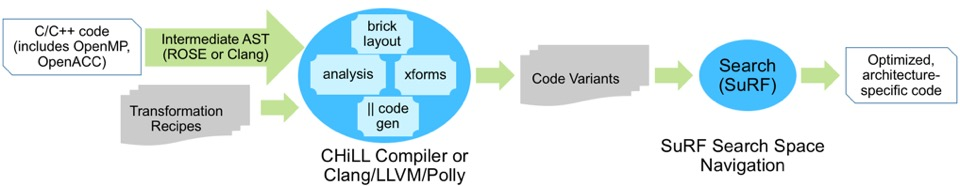
\includegraphics[width=.8\textwidth]{projects/2.3.2-Tools/2.3.2.10-PROTEAS-YTUNE/YTune-solution.jpg}
% 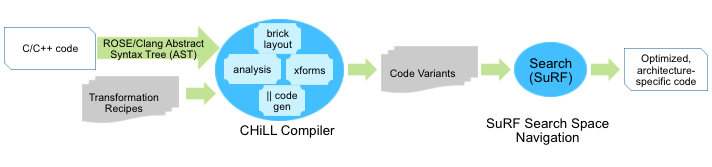
\includegraphics[width=.8\textwidth]{YTune-solution.png}
% \includegraphics[width=.8\textwidth]{PastedGraphic-1.png    }
\end{center}
\caption{Y-TUNE Solution Approach.}
%\caption{S.}                                                                                                                              
%\end{wrapfigure}                                                                                                                          
\end{figure}

%\end{document}

\newpage
\subsubsection{SOLLVE} 

%% {\itshape
%% 
%% 	\begin{enumerate}
%% 	\item Rename this file to your project WBS-projectname.tex, for example 2.3.3.01-XSDK4ECP.tex.
%% 	\item Complete this template for your project.  Limit your text to two pages, not counting citations.  
%% 	\item Please avoid changing the content of main.tex.  
%% 	\item Put any references in a .bib file with the same root name, for example 2.3.3.01-XSDK4ECP.bib.
%% 	\item Remember to include any image files you reference in your text.
%%     \item The files 2.3.3.01-XSDK4ECP.tex, 2.3.3.01-XSDK4ECP.bib and xSDK-diagram.jpeg are included as examples for your reference.  You can remove them from what you upload.
%% 	\end{enumerate}
%% }


\paragraph{Overview}
OpenMP is a directive-based API for intra-node programming that is widely used  in ECP applications. Implementations of OpenMP and  tools to facilitate OpenMP application development.are available in all DOE LCFs.  
The specification is supported by a stable community of vendors, research labs, and academics who
participate in the efforts of the  OpenMP Architecture Review Board (ARB) and its Language Committee to evolve its features.
The mission of the SOLLVE project is to further enhance  OpenMP and its implementations to meet the performance and productivity goals of ECP applications. 

SOLLVE has identified open ECP application software requirements, developed features and/or implementation technology to address them, and created use cases that motivate the need for enhancements. 
 The project continues to identify needs and works to standardize them via 
%In addition to 
active participation in the deliberations of the Language Committee.  
%SOLLVE has moreover produced 
% prototype
%implementations of key new features to support their rapid adoption.

The project is  developing a verification and validation (V\&V) suite to assess implementations and
enable evaluations by DOE  facilities. It is constructing a high-quality,  robust 
OpenMP implementation based on the LLVM compiler. 
%%% BC put in suitable place: resolution of various interoperability 
 SOLLVE plays a critical
role in specifying, implementing, promoting, and deploying functionality
that will enable ECP application developers to reach their goals using OpenMP.
%The project will demonstrate the high impact of new features via their use in selected
%ECP applications.

\paragraph{Key  Challenges}
%\textit{Describe what is hard to do, why it is challenging.}
%need more features, need more implementations (with quality)
Gaps in OpenMP functionality exist as a result of the rapid evolution of node architectures and  base programming languages, as well as a lack of focus on performance portability before version 5.0.  
 Since vendor representatives dominate the  OpenMP Language Committee, effort is needed  to secure their support with regard to the scope of the API, as well as  the syntax and semantics of new features.

%large feature set, many new features are important for ECP
The API has greatly expanded in recent years as some of these gaps are closed, placing a large burden on its implementers. 
The timely provision of  robust implementations of new features that are critical for ECP is therefore particularly challenging.
%%Must we delete this line?
For performance portability, consistent approaches in multiple implementations is highly desirable. Interoperability concerns have emerged as a  new challenge.
 
 %need help to get good performance. 

Given the lack of availability of implementations with features that target accelerators, many existing codes have used alternative APIs for GPUs: a significant effort will be required to replace those approaches by OpenMP. A broad effort is required to develop and apply best practices for new features and platforms. 

\paragraph{Solution Strategy}
We address the challenges by focusing on the following primary activities:

\begin{enumerate}
\item {\bf Application requirements}
Ongoing in-depth interactions with selected ECP application teams have resulted in a list of required extensions, some of which have been met by the recent 5.0 specification.  New needs are being identified. This work informs all other project activities by producing use cases, detailed feedback and example codes. It moreover contributes to the OpenMP Examples document. 
\item {\bf OpenMP specification evolution}
Members of the SOLLVE project are active participants in the OpenMP Language committee.  The project creates early prototypes for new features based on ECP use cases, develops concrete proposals and submits them for standardization. Several proposed features  were included in OpenMP 5.0, ratified November 2018. More are under development for version 5.1.
\item {\bf LLVM  Compiler}
SOLLVE implements new OpenMP features in the LLVM compiler and develops analyses and transformations that enhance, and provide consistency to, OpenMP performance. Its open source solutions may be leveraged in vendor compilers.
The compiler is available on LCF platforms.
\item {\bf Lightweight OpenMP runtime}
The BOLT runtime, built upon ultra-lightweight threading, addresses the need for efficient nested parallelism and improved task scheduling, it develops better support for interoperability with MPI. BOLT is integrated and delivered with the project's LLVM compiler. 
\item {\bf Validation and Verification (V\&V)} 
A V\&V suite is being implemented that allows vendors, users and facilities to assess the coverage
and standard compliance of OpenMP implementations. A ticket system for bug reporting and inquiries has also been deployed to facilitate interaction with end users.
\item{\bf Training and Outreach}
 Tutorials and webinars are delivered to provide information on OpenMP features and their usage, as well as updating on the status of  %their support in vendor and open source 
 implementations. Deeper interaction with application programmers via hackathons supports the development of ECP codes using all available OpenMP features.
%  also provides immediate feedback to compiler and tool developers as the application teams experiment with the use of new features.  
\end{enumerate}
%%revision needed starting here: publications from IWOMP, Lingda, etc.


\paragraph{Recent Progress}
Figure \ref{fig:sollve-update} shows the latest progress on the 5 core SOLLVE
thrust areas. The {\bf training and outreach} activity is a
cross-cutting effort which is supported by resources from SOLLVE and  ECP Broader Engagement,
 with contributions by external collaborators, notably Lawrence Berkeley National
Laboratory.   
%Oak Ridge and Delaware are not external so I commented this out in the hope it can benefit the figure
%project and
%external partners, namely collaborators from Lawrence Berkeley National
%Laboratory, Oak Ridge, University of Delaware and other academic institutions.
A number of articles have also been published
as part of the SOLLVE
effort~\cite{openmp-tr6,zinenko.cc.2018,vandv2019,
tregion, Mishra:2019:KFA:3314872.3314915,
udm, loopTransPragmas, DBLP:conf/iwomp/SreenivasanJHBS19,
DBLP:conf/iwomp/ScoglandSOHES19, DBLP:conf/iwomp/0001WLSS19,
DBLP:conf/iwomp/KaleIKKC19, Bak2019OptimizedEO, lsrt, boltPACT19}.


%% The value that SOLLVE brings to ECP is observed in the ease of leveraging
%% different OpenMP features related to data mappings, parallelism exposure (e.g.
%% {\bf concurrent} or {\bf simd} directives) and control (affinity), runtime
%% scheduling and accelerator (device) offloading (e.g. GPUs or FPGAs).

\begin{figure}[t]
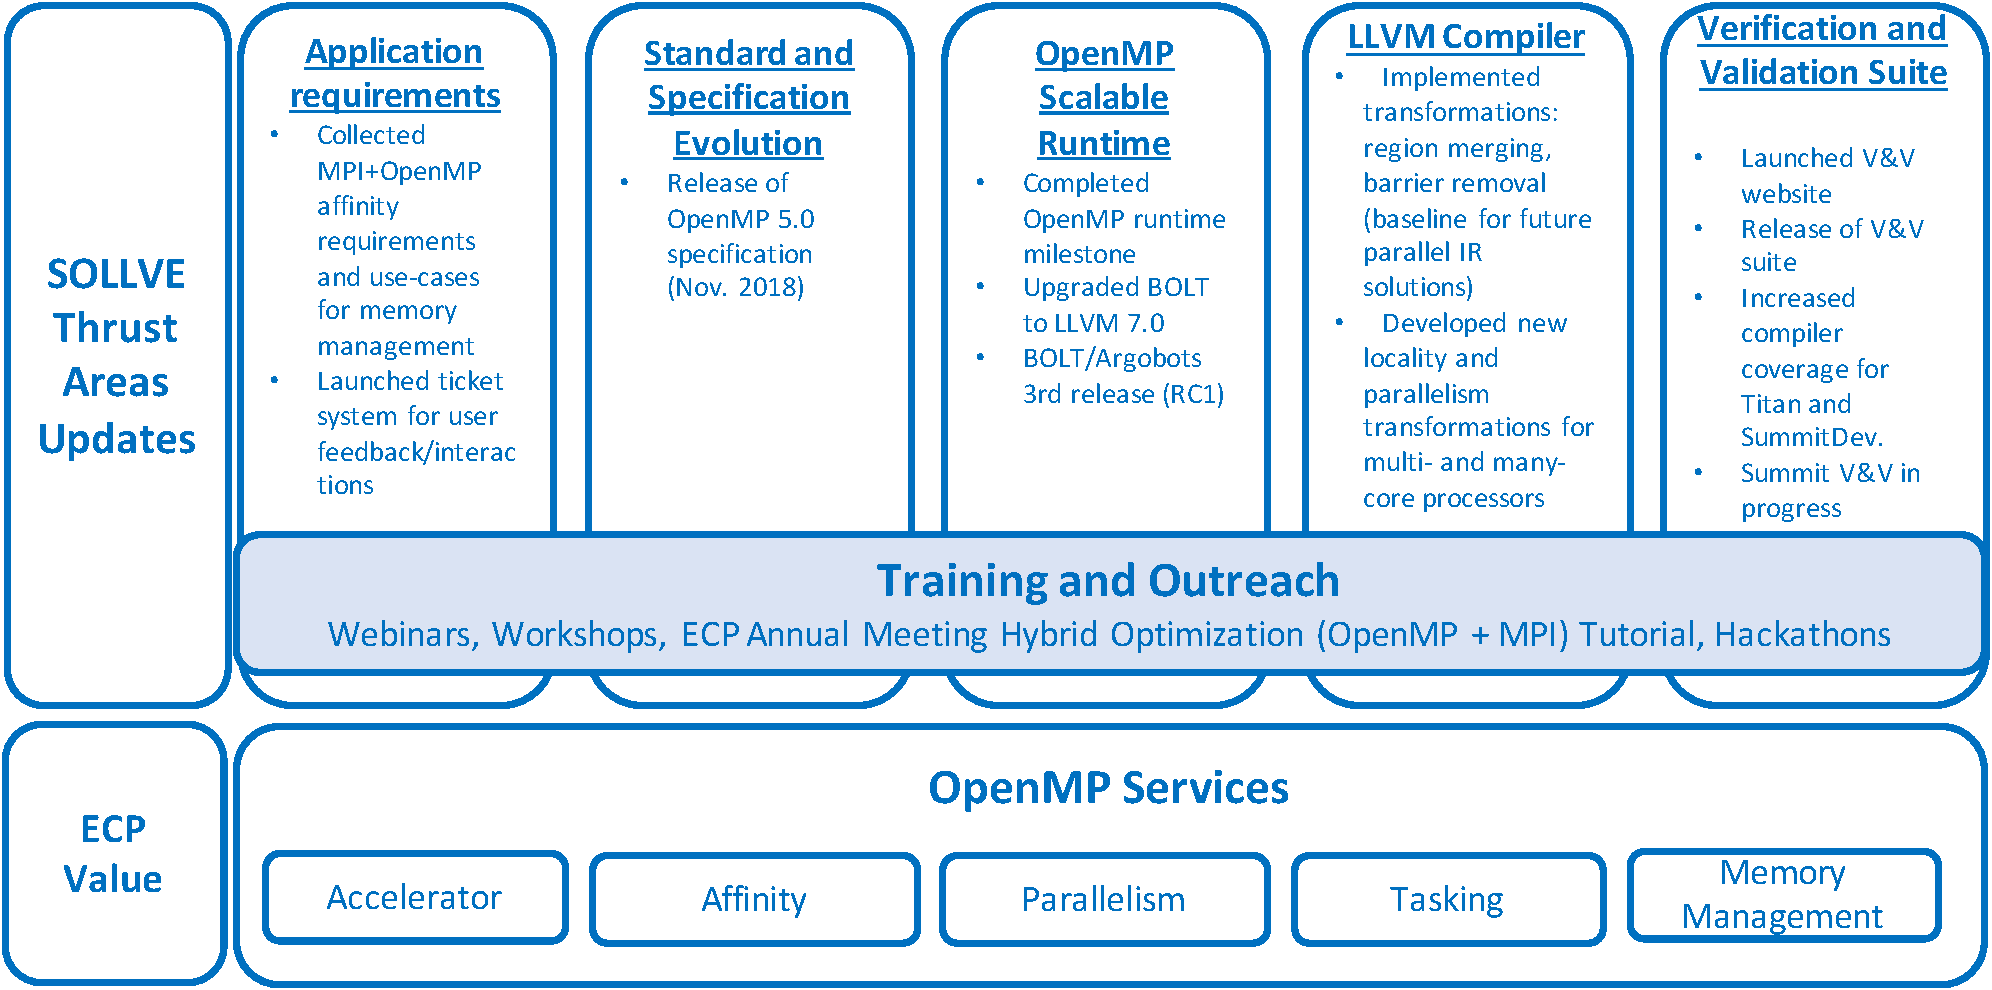
\includegraphics[width=1.0\linewidth,height=9.1cm]{SOLLVE-progress}
\caption{\label{fig:sollve-update}SOLLVE thrust area updates}
\end{figure}
%\textit{Describe what you have done recently.  It would be good to have some kind of figure or diagram in this section.}

\paragraph{Next Steps}
The following next steps are planned:
\begin{itemize}
\item Applications: Continue to interact with ECP applications teams, evaluate implementations of new features and explore new requirements; 
% create mini-apps to help evaluate OpenMP accelerator support; 
 identify best practices for the use of OpenMP on accelerators;
%for memory management API and concurrent parallel construct; prepare and coordinate %OpenMP webinar focusing on memory management, deep copy and tasking. Spack %package development and deployment with applications. 
\item OpenMP specification: Continue work toward the next version of the standard via ECP-motivated feature development and participation in the OpenMP Language Committee: version 5.1 is already well under way and is due for release November 2020;
%Next face-to-face meeting in January 2019; ratify and vote latest memory management %features and mappers, vote on examples, add to loop scheduling and tasking for affinity %research. 
\item LLVM compiler: Improve performance of device offloading and optimize generation of code within target devices; generalize to enable reuse across multiple offloading architectures; develop infrastructure to support integration of Fortran front end; increase parallel region performance; 
%develop new optimizations for loop transformations; refine Clang based implementation of data layout transformations for OpenMP offloading; improve general testing; evaluate on Summit and other ECP systems. 
\item OpenMP runtime: provide support for 5.0 spec; improve performance of MPI+OpenMP codes; address broader set of interoperability challenges; address advanced tasking requirements;
% and MPI implementations
\item V\&V suite: Continue expanding the coverage of the V\&V Suite, with main focus on 4.5 features;  expand Fortran tests; work with ARB Examples Committee; improve ALCF toolchains;
\end{itemize}

%\textit{Describe what you are working on next.}

\subsubsection{\stid{2.11} Argobots: Flexible, High-Performance Lightweight Threading }

\paragraph{Overview}

Efficiently supporting massive on-node parallelism demands highly
flexible and lightweight threading and tasking runtimes. At the
sametime, existing lightweight abstractions have shortcomings while
delivering generality and specialization.  Our group at Argonne
developed a lightweight, low-level threading and tasking framework,
called Argobots.  The key focus areas of this project are: (1) To
provide a framework that offers powerful capabilities for users to
allow efficient translation of high-level abstractions to low-level
implementations. (2) To provide interoperability with other
programming systems such as OpenMP and MPI as well as with other
software components (e.g., I/O services). (3) To provide a programming
framework that manages hardware resources more efficiently and reduce
interference with colocated applications.

\paragraph{Key Challenges}

Several user-level threading and tasking models have been proposed in
past to address the shortcomings of OS-leve threads, primarily with
respect to cost and flexibility. Their lightweight nature and flexible
generic interface play an important role at managing efficiently the
massive concurrency expected at the Exascale level.  Existing
user-level threading and tasking models, however, are either too
specific to applications or architectures or are not as powerful or
flexible. Existing runtimes tailored for generic use \cite{GNUPth,
  PLDI97_Taura, COSET05_Thibault, COB14_Nakashima, MTAAP08_Wheeler,
  PPoPP99_Taura, SenSys06_Dunkels, TBB1, EuroPar08_Perache} are
suitable as common frameworks to facilitate portability and
interoperability but offer insufficient flexibility to efficeintly
capture higher-level abstractions, while specialized runtimes
\cite{ATC02_Adya, SolarisThreads, SOSP03_von_Behren, StateThreads,
  PLDI07_Li, MTAAP09_Porterfield, WMPP05_Cuvillo, IntelOMP, Nanos++,
  LCPC96_Kale, PACT14_Treichler} are tailored to specific environment.

\paragraph{Solution Strategy}

Argobots offers a carefully designed execution model that balances
generality of functionality with providing a rich set of controls to
allow specialization by end users or high-level programming models
\cite{seo2018}.  Delivering high performance in Argobots while
providing a rich set of capabilities is achieve by heavily optimizing
critical paths as well as by exposing configuration knobs and a rich
API that allow users to trim unnecessary costs. Furthermore, Argobots
honors high degrees of expressibility through three key aspects:

\begin{enumerate}

\item Capturing the requirements of different \emph{work units}, which
are the most basic manageable entities. Work units that require
private stacks and context-saving capabilities, referred to as
\textit{user-level threads} (ULTs, also called \textit{coroutines} or
\textit{fibers}), are fully fledged threads usable in any context.
\emph{Tasklets} do not require private stacks. They are more
lightweight than ULTs because they do not incur context saving and
stack management overheads.  Tasklets, however, are restrictive; they
can be executed only as atomic work units that run to completion
without context switching.

\item Exposing hardware computational units through \emph{execution
streams} as OS-level threads to execute work units. Unlike existing
generic runtimes, ESs are exposed to and manageable by users.

\item Allowing full control over \emph{work unit management}.  Users
can freely manage \emph{scheduling} and mapping of work units to ESs
through \emph{thread pool} management, and thus achieving the desired
behavior. Figure~\ref{fig:sollve-argobots} illustrates the various
building blocks in the Argobots framework and the interactions between
them to build a hypothetical system.

\end{enumerate}

\begin{figure}[htb]
  \centering
  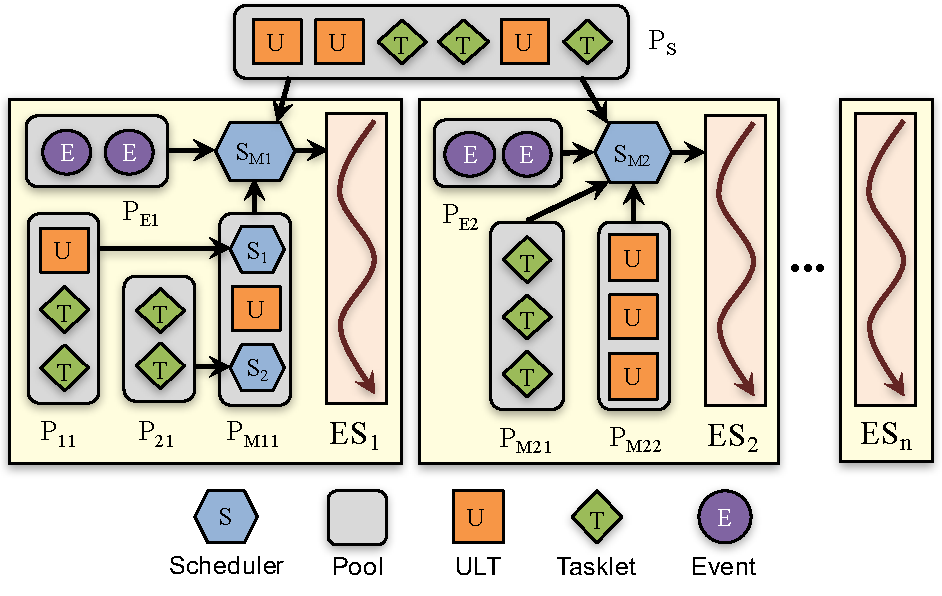
\includegraphics[height=3in]{projects/2.3.2-Tools/2.3.2.11-SOLLVE/SOLLVE-ARGOBOTS.pdf}
  \caption{\label{fig:sollve-argobots}Argobots execution model}
\end{figure}


\paragraph{Recent Progress}

Argobots was built from the ground up focusing on fast critical paths
and a flexibly API. Several programming systems, such as OpenMP, Cilk,
and Charm++, have been demonstrated to run efficiently using Argobots
as their underlying threading layer. Our most recent successful
integration is our BOLT OpenMP runtime that demonstrated significant
improvements over commercial and open source production OpenMP
runtimes. Furthermore, composing multiple programming systems or
libraries proved to be more efficient using Argobots as the
interoperation layer as opposed to a OS-level interaction. This was
demonstrated by achieving performance when multiple application
threads access the MPI stack or when applications are collocated I/O
services that incur significant overheads to deliver high response
times.

Argobots featured three software releases and publications in top tier
venues in the field. It has been recently extended with new thread
management techniques, called \emph{dynamic promotion}, that adapt to
application needs in terms of suspension as an alternative to
user-hinted distinction between work units. This effectively improves
user productivity while relying on runtime adaptation to deliver high
performance~\cite{iwasaki2018}. Recently, the Argobots API was also
extended to facilitate better resource utilization under idleness, has
been hadned with performance optimizations and stabilization, and
experienced improvements in the debugging infrastructure.

\paragraph{Next Steps}

Argobots continues to grow in terms of features, integration or
composition with other systems, and hardening. Below is a short
list of the major ongoing and planned extensions and optimizations.

\begin{enumerate}

\item Extend and optimize Argobots for BOLT needs. While Argobots is
used by several systems, BOLT is one of those that rely heavily on
Argobots to perform well and offer necessary abstractions. We plan to
continue involving Argobots in our BOLT optimization process and
extend Argobots and optimize it accordingly.

\item Investigating composition challenges and opportunities outside
MPI. Our investigation of using Argobots as the interoperability layer
between heterogeneous software systems involved mostly MPI (given its
prominence) and I/O services to some extent. This investigation is
only preliminary; several HPC programming systems and libraries rely
on OS-level threads and their composition might benefit for Argobots
and warrants investigation.

\end{enumerate}

\subsubsection{\stid{2.11} BOLT: Lightning Fast OpenMP}\label{subsubsect:bolt}

\paragraph{Overview}

OpenMP is central for several applications that target Exascale,
including ECP applications, to exploit on-node computational
resources.  Unfortunately, current production OpenMP runtimes, such as
those that ship with Intel and GNU compilers, are inadequate for the
massive and fine-grained concurrency expected at the Exascale level.
These runtimes rely on heavy-handed OS-level threading strategies that
incur significant overheads at fine-grained levels and exacerbate
interoperability issues between OpenMP and internode programming
systems, such as MPI and OpenSHMEM.  Our solution is a production
quality OpenMP runtime (called BOLT) that leverages user-level threads
instead of OS-level threads (e.g., Pthreads).  Due to their
lightweight nature, managing and scheduling user-level threads incurs
significantly less overheads.  Furthermore, interoperability between
BOLT and internode programming systems opens up new optimization
opportunities by promoting asynchrony and reducing hardware
synchronization (atomics and memory barriers).  Initial studies on
this proposal can be found in \cite{amer2018, ccgrid, ppopp}. This
report briefly summarizes the issues in OpenMP runtimes that rely on
OS-level threading, describes BOLT as the solution to this challenge,
the current status in the BOLT effort, and the next steps for further
improvements.

\paragraph{Key Challenges}

The growing hardware concurrency in High Performance Computing (HPC)
cluster nodes is pushing applications to chunk work more fine-grained
to expose parallelism opportunities.  This is often achieved through
nested parallelism either in the form of parallel regions or by
explicit tasks.  Nested parallel regions can potentially cause
oversubscription of OS-level threads to CPUs and thus lead to
expensive OS-level thread management.  Such heavy costs usually
outweigh the benefits of increased concurrency and thus compel the
OpenMP programmer to avoid nested parallel regions altogether.  Such
workaround, however, not only causes poor resource utilization from
insufficient parallelism but is also not always possible.  For
instance, the nested level could be outside the control of the user
because it belongs to an external library that also uses OpenMP
internally.  Internode programming systems, such as MPI and OpenSHMEM,
are not aware of OpenMP semantics, such as the notion of an OpenMP
task.  What these internode systems understand is the low-level
threading layer used by OpenMP, such as Pthreads.  This threading
layer serves as the interoperability medium between OpenMP and the
internode programming system and has a direct impact on performance.
It is notoriously known that OS-level thread safety in production MPI
libraries suffers significant performance issues. While continued
progress on improving OS-level thread safety in these important
internode programming systems is crucial for traditional
interoperability, we propose in this work exploring an orthogonal
direction that assumes a more lightweight interoperability layer.

\paragraph{Solution Strategy}

Both fine-grained parallelism and interoperability issues suffer from
the heavy nature of working at the level of OS threads.  Our solution
to both challenges leverages user-level threads.  Using user-level
threads as the underlying threading layer for the OpenMP runtime
offers a significantly better trade-off between high concurrency and
thread management overheads.  This allows users to generate
fine-grained concurrency and oversubscription without worrying about
the performance collapse that is observed in current OpenMP runtimes.
Our OpenMP runtime, BOLT, is derived from the LLVM OpenMP runtime and
leverages Argobots, a highly optimized lightweight threading library,
as its underlying threading layer.  OpenMP threads and tasks are
spawned as Argobots work units and nested parallel regions are managed
through an efficient work-stealing scheduler.  Furthermore, new
compiler hints and runtime optimizations have been developed to allow
reducing thread management overheads even further~\cite{iwasaki2018}.
Interoperability improvements have also been demonstrated by having
BOLT interoperate with an MPI library (MPICH) through the Argobots
threading layer rather than OS-level threads.  Results showed that
this approach allows better communication progress and outperforms the
traditional Pthreads-level interaction~\cite{seo2018}.

\paragraph{Recent Progress}

Our recent development of BOLT mainly focuses on efficient OpenMP
thread scheduling and management~\cite{BOLT}. BOLT takes substantial
advantage of its base implementation of LLVM OpenMP in terms of ABI
compatibility and coverage of functionalities, while we found the
necessity of further performance optimizations to fully exploit
fine-grained OpenMP parallel regions. After simple replacement of
Pthreads call sites with Argobots functions, we adopted several
resource management optimizations to reduce contentions and promote
reuse of resources. Thanks to low-level scheduling functions exposed
by Argobots, BOLT could implement OpenMP affinity tailored to a
ULT-based runtime. Our study also  the importance of a thread
coordination algorithm: it determines how to synchronize with other
threads (e.g., busy wait or suspension). To get the optimal
performance, existing runtime systems need to tune the wait policy
parameter based on the level of oversubscription, while our advanced
thread coordination algorithm in BOLT transparently keeps good
performance regardless of the degree of thread oversubscription. As
shown in Figure~\ref{fig:sollve-bolt}, BOLT achieves similar
performance compared with leading state-of-the-art OpenMP runtimes
under flat parallelism, while outperforming all the existing runtimes
under nested parallelism.

\begin{figure}[t]
  \centering
  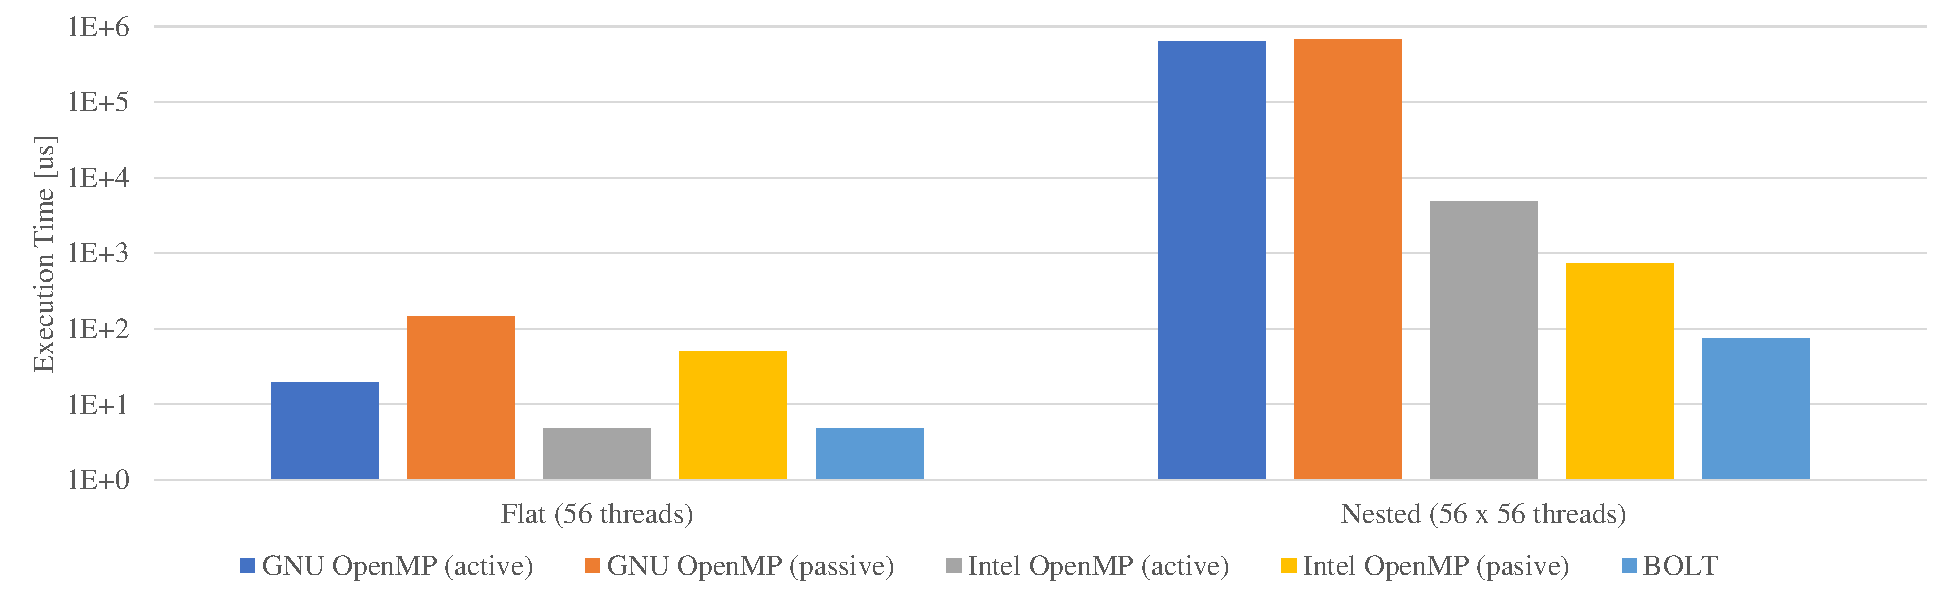
\includegraphics[width=0.9\columnwidth]{projects/2.3.2-Tools/2.3.2.11-SOLLVE/SOLLVE-BOLT.pdf}

  \caption{\label{fig:sollve-bolt}Performance of parallel regions on a
two-socket Intel Skylake machine (56 cores in total). GNU OpenMP 8.0
and Intel OpenMP 17.2.174 are used. The flat benchmark creates 56
OpenMP threads while the nested 56 OpenMP threads each of which opens
an inner parallel region with 56 threads. We changed the wait policy
for GNU and Intel OpenMP. See the paper \cite{BOLT} for details.}

\end{figure}

We note that design and implementation of BOLT are highly regarded in
the HPC community. The most significant achievement is the Best Paper
Award at PACT '19; our paper on BOLT, titled ``BOLT: Optimizing OpenMP
Parallel Regions with User-Level Threads''~\cite{BOLT} won a Best
Paper Award at the 28th international conference on Parallel
Architectures and Compilation Techniques (PACT '19), which is
considered to be a top tier venue in this field.

The latest BOLT 1.0rc2 has been upgraded to be compatible with LLVM
OpenMP 9.0, which further improves performance and functionalities
especially for GPU offloading. We also created a development branch
that keeps reflecting the latest changes in the LLVM OpenMP's master
branch so that BOLT users can try the up-to-date features with ULT
support. Interaction and integration are a critical piece for the BOLT
project. Our effort in the SOLLVE Spack package, which was one of the
SOLLVE milestones, aims at a tighter integration with the other
components of the SOLLVE project. Our efforts include interaction and
evaluation with (1) ECP applications that have fine-grained
parallelism such as nested parallel regions and tasking (e.g., ECP
SLATE) and (2) runtime systems via the Argobots layer (for example,
MPICH and Open MPI) that can take advantage of ULT's lightweight
synchronization for resource management.

\paragraph{Next Steps}

One of the largest advantages of BOLT is an underlying lightweight
thread implementation, flexible scheduling, and high interoperability
thanks to Argobots. The following list includes our next plans:

\begin{enumerate}

\item Investigates opportunities of utilizing lightweight threads for
other optimizations in the context of OpenMP. BOLT successfully
enhanced performance of OpenMP threads, while it remains unexplored
how BOLT could elevate performance of other parallel units (e.g.,
data-dependent tasking and GPU offloading). We are planning to
investigate room for optimizations and implement them with
evaluation.

\item Improves the interoperability with MPI runtimes. Although the
basic scheme is provided via the Argobots layer, its optimization is
premature. In addition to improvement of the interoperability between
MPI and Argobots, we will investigate an OpenMP-specific
interoperability issue if exists.

\item Collaborates with more applications and users. BOLT has gained
the attention of the HPC community, but its reach and impact remain
limited. In order to find potential room for optimizations and
evaluate the performance of BOLT in real workloads, we further
investigate other applications, including ECP ones, that BOLT can
benefit.

\end{enumerate}

\newpage
\subsubsection{\stid{2.12} Flang}\label{subsubsect:flang}

\paragraph{Overview}

The Flang project provides an open source Fortran
\cite{iso-fortran-2004} \cite{iso-fortran-2010} \cite{iso-fortran-2018}
compiler.  The project was recently formally accepted as a component
of the LLVM Compiler Infrastructure (see \url{http://llvm.org})~\cite{llvm:homepage}.
Leveraging LLVM, Flang will provide a cross-platform Fortran solution available to
ECP and the broad, international LLVM community. The goals of the project include
extending support to GPU accelerators and target Exascale systems, and supporting
LLVM-based software and tools R\&D of interest to a large deployed
base of Fortran applications.

LLVM's growing popularity and wide adoption within the
broader HPC community make it an integral part of the modern software ecosystem.
This project provides the foundation for a Fortran solution that will complement and interoperate with the
Clang/LLVM C++ compiler.  We aim to allow Fortran to grow into a
modernized open source form that is stable, has an active footprint
within the LLVM community, and will meet the needs of a broad
scientific computing community.

\paragraph{Key Challenges}
Today there are several commercially-supported Fortran compilers,
typically available on only one or a few platforms.  None of these are
open source.  While the GNU gfortran open source compiler is available
on a wide variety of platforms, the source base is not modern
LLVM-style C++ and the GPL open source license is not compatible with
LLVM, both of which can impact broader community participation and adoption.

The primary challenge of this project is to create a source base with
the maturity, features, and performance of proprietary solutions with
the cross-platform capability of GNU compilers, and which is licensed
and coded in a style that will be embraced by the LLVM community.
Additional challenges come from robustly supporting all Fortran
language features, programming models, and scalability required for effective use on Exascale systems. 

\paragraph{Solution Strategy}

With the adoption of Flang into the LLVM community as an official subproject,
our strategy focuses on development and delivery of a solid, alternative Fortran
compiler for DOE's Exascale platforms.  In addition, we must be good shepherds
within the LLVM community to establish and grow a vibrant community of our own. This is
in the best interest of ECP as well as the long-term success of Fortran in the
LLVM community and the many industry and academic projects that rely upon it. 

Our path to success will rely on significant testing across not only
the various facilities but also across a very broad and diverse set of applications.
Given the relatively early development stage of Flang, this testing will be paramount 
in the delivery of a robust infrastructure to ECP and the broader community. 

\paragraph{Recent Progress}

After several years of effort and support from NNSA, Flang was successfully ``adopted''
by the LLVM community and is currently in the process of making a transition from a
stand-alone git repository to an LLVM hosted project.  This represents a significant
result and the current code is available as ``F18'' via GitHub:

\begin{center}
\url{https://github.com/flang-compiler/f18}
\end{center}

When it officially completes the move to LLVM's repository it will be renamed ``Flang''. 

The current capabilities of ``F18'' include the full Fortran 2018
standard and OpenMP 5.X syntax and semantics.  As part of the
development of the parsing and semantic analysis portions of the
front-end, over five million lines of Fortran code has been
successfully processed. We will continue and expand this level of
testing as we near the completion of the first full (sequential)
compiler early in the 2020 calendar year.  This effort includes the
use of a Fortran-centric intermediate representation (Fortran IR --
``FIR'') that leverages recent activities within Google
on \href{Multi-Level Intermediate Representations}
{https://www.blog.google/technology/ai/mlir-accelerating-ai-open-source-infrastructure/}
(MLIR) for use with the implementation of FIR.

\paragraph{Next Steps}
Our short-term priorities are focused on the completion of the
sequential compiler, the creation of a significant testing
infrastructure, and helping to lead the interactions and overall
discussions within the LLVM community.  Longer term efforts
will shift to support OpenMP 5.X features critical to ECP applications
on the target Exascale platforms.  We are actively exploring finding a
common leverage point between Clang's current OpenMP code base and
Flang.  This would enable the reuse of existing code versus writing
everything from scratch in Flang.  We see this as a critical path
forward to enabling a timely release of a node-level parallelizing
compiler for ECP.  Additional work will focus on features that would
benefit Fortran within the LLVM infrastructure as well as general and
targeted optimization and analysis capabilities.


\newpage


\subsection{\mathlibs}
This section present projects in \mathlibs.
\newpage
\subsubsection{\stid{3.01} xSDK4ECP} 
\paragraph{Overview} The xSDK4ECP project is creating a value-added aggregation of DOE math and scientific libraries through the {\em xSDK} (Extreme-scale Scientific Software Development Kit)~\cite{xsdk:homepage}, which increases the combined usability, standardization, and interoperability of these libraries as needed by ECP. The project focuses on community development and a commitment to combined success via quality improvement policies, better build infrastructure, and the ability use diverse, independently developed xSDK libraries in combination to solve large-scale multiphysics and multiscale problems.  We are extending draft xSDK package community policies and developing interoperability layers among numerical libraries in order to improve code quality, access, usability, interoperability, and sustainability. Focus areas are (1) coordinated use of on-node resources, (2) integrated execution (control inversion and adaptive execution strategies), and (3) coordinated and sustainable documentation, testing, packaging, and deployment.

xSDK4ECP is needed for ECP because it enables ECP apps such as ExaAM and ExaWind to seamlessly leverage the entire scientific libraries ecosystem.  For example, ExaWind has extremely challenging linear solver scaling problems.  xSDK4ECP provides access to all scalable linear solvers with minimal changes.  xSDK4ECP is also an essential element of the product release process for ECP ST.  xSDK4ECP provides an aggregate build and install capability for all ECP math libraries that supports hierarchical, modular installation of ECP software.  Finally, xSDK4ECP provides a forum for collaborative math library development, helping independent teams to accelerate adoption of best practices, enabling interoperability of independently developed libraries and improving developer productivity and sustainability of the ECP ST software product.

\paragraph{Key Challenges}
The complexity of application codes is steadily increasing due to more sophisticated scientific models.  While some application areas will use Exascale platforms for higher fidelity, many are using the extra computing capability for increased coupling of scales and physics.  Without coordination, this situation  leads to difficulties when building application codes that use 8 or 10 different libraries, which in turn might require additional libraries or even different versions of the same libraries.

The xSDK represents a different approach to coordinating library development and deployment.  Prior to the xSDK, scientific software packages were cohesive with a single team effort, but not across these efforts. The xSDK goes a step further by developing community policies followed by each independent library included in the xSDK.  This policy-driven, coordinated approach enables independent development that still results in compatible and composable capabilities.

\paragraph{Solution Strategy}

The xSDK effort has two primary thrusts:
\begin{enumerate}
	\item \textbf{Increased interoperability:} xSDK packages can be built with a single Spack package target.  Furthermore, services from one package are accessible to another package.
	\item \textbf{Increased use of common best practices:}  The xSDK has a collection of community policies that set expectations for a package, from best design practices to common look-and-feel.
\end{enumerate}

xSDK interoperability efforts began first with eliminating incompatibilities that prohibited correct compilation and integration of the independently developed libraries.  These issues include being able to use a common version of a library such as SuperLU by PETSc and Trilinos.  The second, and ongoing phase is increased use of one package's capabilities from another.  For example, users who build data objects using PETSc can now access Trilinos solvers without copying to Trilinos data structures.

xSDK community package policies~\cite{xsdk-policies:homepage,
xSDK-community-package-policies2018} are a set of minimum requirements (including topics of configuring, installing, testing, MPI usage, portability, contact and version information, open source licensing, namespacing, and repository access) that a software package must satisfy in order to be considered xSDK compatible. The designation of xSDK compatibility informs potential users that a package can be easily used with others. 

xSDK community installation policies~\cite{xSDK-community-installation-policies2017} help make configuration and installation of xSDK software and other HPC packages as efficient as possible on common platforms, including standard Linux distributions and Mac OS X, as well as on target machines currently available at DOE computing facilities (ALCF, NERSC, and OLCF) and eventually on new Exascale platforms.

Community policies for the xSDK promote long-term sustainability and interoperability among packages, as a foundation for supporting complex multiphysics and multiscale ECP applications. In addition, because new xSDK packages will follow the same standard, installation software and package managers (for example, Spack~\cite{gamblin+:sc15}) can easily be extended to install many packages automatically.


\paragraph{Recent Progress}

Figure~\ref{fig:xsdk-schematic} illustrates a new {\em Multiphysics
	Application C}, built from two complementary applications that can
readily employ any libraries in the xSDK, shown in green.  Current xSDK member packages (xSDK-0.4.0, released December 2018) are the four founding libraries
(hypre~\cite{hypre:homepage}, PETSc~\cite{petsc:homepage}, SuperLU~\cite{superlu:homepage}, and Trilinos~\cite{trilinos:homepage}), three libraries added in xSDK-0.3.0, released December 2017 (MAGMA~\cite{magma:homepage}, MFEM~\cite{mfem:homepage}, and SUNDIALS~\cite{sundials:homepage}), and ten more libraries added in this release, including seven with DOE support (AMRex~\cite{amrex:homepage}, DTK~\cite{dtk:homepage}, Omega\_h~\cite{omega_h:homepage}, PLASMA~\cite{plasma:homepage}, PUMI~\cite{pumi:homepage}, STRUMPACK~\cite{strumpack:homepage}, and Tasmanian~\cite{tasmanian:homepage}) and three in the broader community (deal.II~\cite{deal.ii:homepage}, PHIST~\cite{phist:homepage}, and SLEPc~\cite{slepc:homepage}).  
Application domain components are represented
in orange.  Of particular note is Alquimia~\cite{alquimia:homepage}, a domain-specific interface
that support uniform access to multiple biogeochemistry capabilities, including
PFLOTRAN~\cite{pflotran:homepage}.  Additional libraries are working toward becoming xSDK member packages and plan to participate in future xSDK releases.
\begin{figure}[htb]
	\centering
	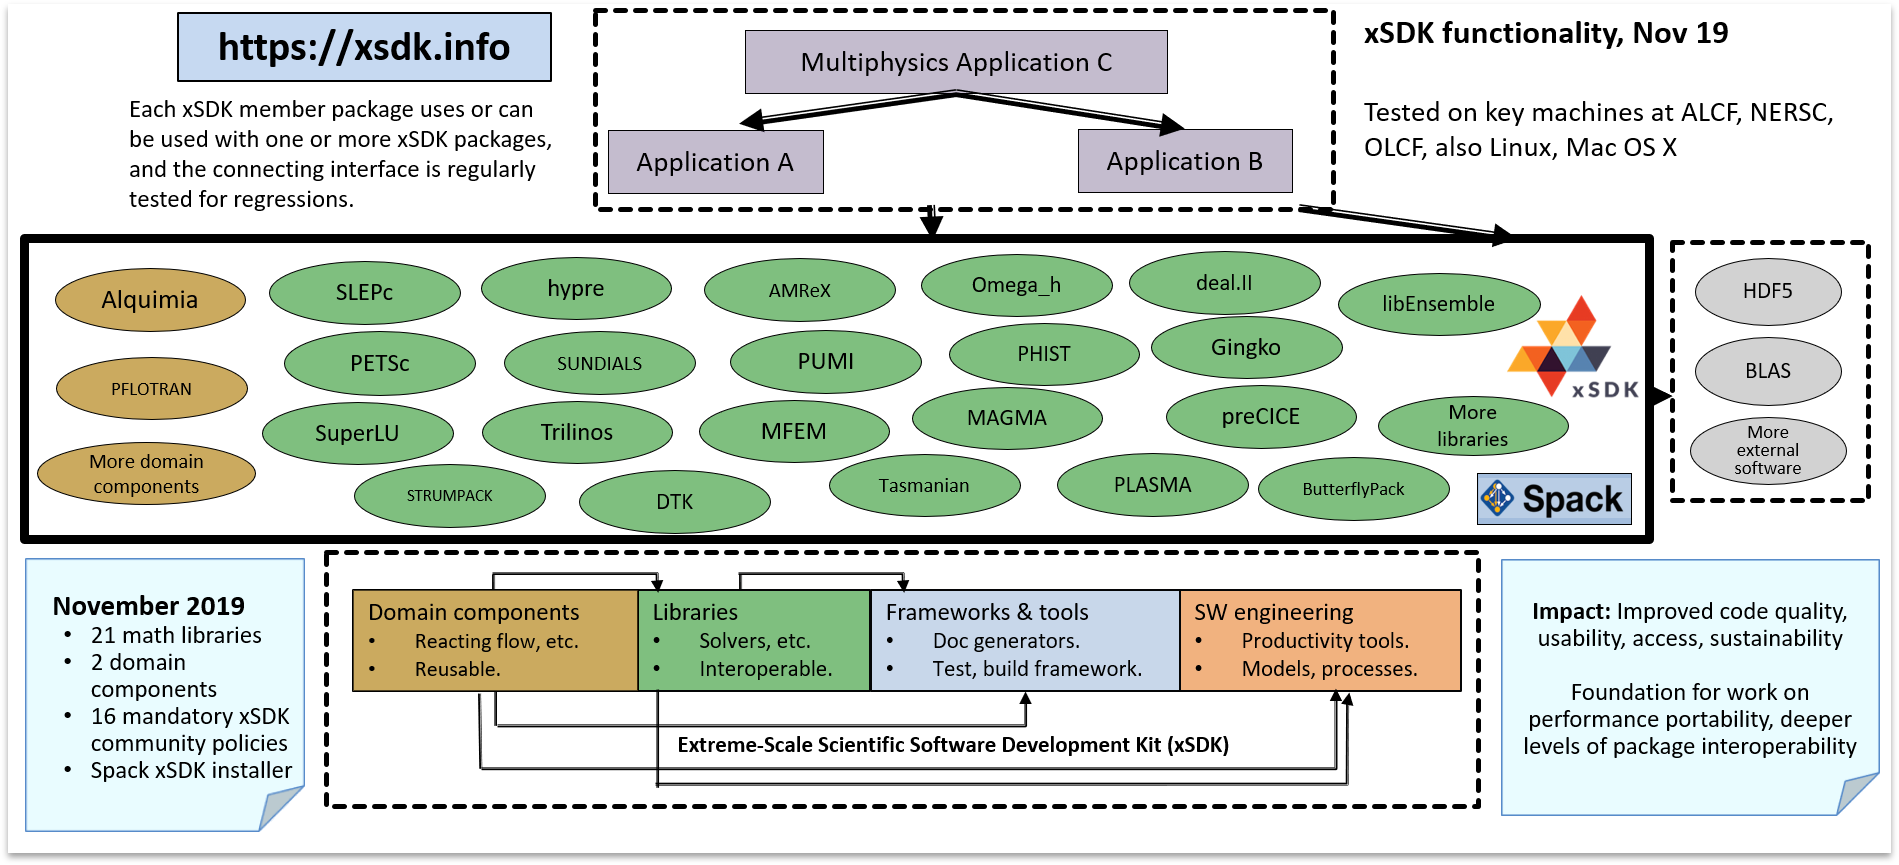
\includegraphics[width=6in]{projects/2.3.3-MathLibs/2.3.3.01-xSDK/xSDK-diagram.png}
	\caption{\label{fig:xsdk-schematic}The December 2018 release of the xSDK contains many of the most popular math and scientific libraries used in HPC.  The above diagram shows how multiphysics and multiscale applications can readily access xSDK packages.}
\end{figure}

% The arrows among the xSDK libraries indicate current support for
% a package to call another to provide scalable linear solvers
% functionality on its behalf.  For example, {\em Application~A} could
% use PETSc for an implicit-explicit time advance, which in turn could
% interface to SuperLU to solve the resulting linear systems with a
% sparse direct solver.  {\em Application~B} could use Trilinos to solve
% a nonlinear system, which in turn could interface to hypre to solve
% the resulting linear systems with algebraic multigrid.  Of course,
% many other combinations of solver interoperability are also possible.
Each xSDK member package uses or can be used with one or more xSDK packages, and the connecting interface is regularly tested for regressions.  
The sites \url{https://xsdk.info/example-usage} and 
\url{https://xsdk-project.github.io/ATPESC2018HandsOnLessons}, as well as
\cite{Klinvex-xSDKTrilinos} provide examples of
xSDK usage, including interoperability among linear solvers in hypre,
PETSc, SuperLU, and Trilinos.


\paragraph{Next Steps}


Our next efforts are:
\begin{enumerate}
	\item \textbf{Include more libraries:} xSDK4ECP will continue efforts to expand the number of participating packages, adapt community policies, and exploit increased interoperability.  We are coordinating with broader SDK efforts and working toward the inclusion of additional domain application packages.
	\item \textbf{Extend application usage:}  xSDK4ECP will continue partnering with application teams to evaluate the effectivness of current functionality and to motivate new capabilities.
% 		\item \textbf{Process control transfer interfaces:} The ever-increasing use of concurrency within the top-level MPI processes requires that computational resources used by an application or library can be transferred to another library. Transfer of these resources is essential for obtaining good performance.  The xSDK project will develop interfaces to support sharing and transfer of computational resources.
	
\end{enumerate}

\newpage
\subsubsection{\stid{3.06} PETSc-TAO} \label{subsubsect:petsc}
\paragraph{Overview} 

Algebraic solvers (generally nonlinear solvers that use sparse linear solvers via Newton's method) and ODE/DAE 
integrators form the core computation of many numerical simulations. No scalable ``black box'' sparse solvers 
or integrators work for all applications, nor single implementations that work well for all scales of 
problem size. Hence, algebraic solver packages provide a wide variety of algorithms and implementations 
that can be customized for the application and range of problem sizes at hand. PETSc~\cite{petsc:homepage,petsc-man} 
is a widely used software library for the scalable solution of linear, nonlinear, and ODE/DAE systems and 
computation of adjoints (sometimes called sensitivities) of ODE systems. We focus on three topics: (1) partially 
matrix-free scalable solvers efficiently use many-core and GPU-based systems; (2) reduced synchronization 
algorithms that can scale to larger concurrency than solvers with synchronization points; and (3) performance 
and data structure optimizations for all the core data structures to better utilize many-core and GPU-based 
systems as well as provide scalability to the Exascale.

The availability of systems with over 100 times the processing power of today's machines compels the utilization 
of these systems not just for a single ``forward solve'' simulation (as discussed above) but rather within a 
tight loop of optimization, sensitivity analysis (SA), and uncertain quantification (UQ). This requires the 
implementation of a new, scalable library for managing a dynamic hierarchical collection of running scalable simulations, where the simulations directly feed results into the optimization, SA, and UQ solvers.  This library, 
which we call libEnsemble, directs the multiple concurrent ``function evaluations'' through the tight coupling 
and feedback described above. This work consist of two parts: (1) the development of libEnsemble and (2) the 
extension of TAO~\cite{tao-man} (our PETSc-based scalable optimization library) with new algorithms and 
software to utilize libEnsemble.

\paragraph{Key Challenges}

A key challenge for for scaling the PETSc/TAO numerical libraries to Exascale systems is that 
traditional ``sparse-matrix-based'' techniques for linear, nonlinear, and ODE solvers, as well 
as optimization algorithms, are memory-bandwidth limited.  Another difficulty is that any 
synchronizations required across all compute units--for example, an inner product or a 
norm--can dramatically affect the scaling of the solvers.

Running an ensemble of simulation requires a coordination layer that handles load balancing and
allows the collection of running simulations to grow and shrink based on feedback. Thus, this 
library must be able to dynamically start simulations with different parameters, resume 
simulations to obtain more accurate results, prune running simulations that the solvers 
determine can no longer provide useful information, monitor the progress of the simulations, 
and stop failed or hung simulations, and collect data from the individual simulations both 
while they are running and at the end.

\paragraph{Solution Strategy}

To address the scalability of the numerical libraries, we are developing new solvers and data 
structures including pipeline Krylov methods that delay the use of the results of inner products 
and norms, allowing overlapping of the reductions and other computation; partially matrix-free 
solvers using high-order methods that have high floating-point-to-memory-access ratios and
good potential to use many-core and GPU-based systems; and in-node optimizations of sparse 
matrix-matrix products needed by algebraic multigrid to better utilize many-core systems
using a thread neutral ``bypass MPI'' approach, which implements default interprocessor 
communication using MPI but bypasses the use of MPI in performance-critical regions 
for higher performance and thereby maintains MPI portability.

Our strategy for coordinating ensemble computations has been to develop libEnsemble
to satisfy our needs.  This library should not be confused with workflow-based 
scripting systems; rather it is a library that, through the tight coupling and 
feedback described above, directs the multiple concurrent ``function evaluations''
needed by optimization, SA, and UQ solvers.

\paragraph{Recent Progress}

In the past year, we have released PETSc 3.10 (available at \url{http://www.mcs.anl.gov/petsc})
that features enhanced GPU support.  In particular, PETSc’s algebraic multigrid (AMG) consists 
of two main components: the setup (coarsening) phase which has both GPU and CPU intensive 
portions and the solve stage which can run largely or completely on the GPU. A key 
requirement is minimizing the amount of communication needed between the CPU 
and GPU during both phases of the computation.  In the PETSc~3.10 release, we 
completed porting key AMG kernels for both phases to GPUs via CUDA, enabling
this code to run on a combination of the CPU and GPU.

\begin{figure}
\centering
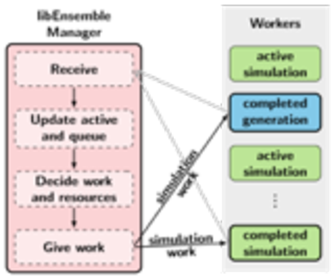
\includegraphics[width=0.3\textwidth]{projects/2.3.3-MathLibs/2.3.3.06-PETSc-TAO/lib_ensemble}
\caption{The libEnsemble control flow showing a manager coordinating workers executing 
calculations of either simulation functions or generation functions.}
\label{fig:petsc-tao-fig}
\end{figure}

We have also developed the libEnsemble API, implemented it in Python, released 
version 0.4 (available at \url{https://github.com/Libensemble/libensemble}),
and provided a Spack installation.

\paragraph{Next Steps}

Our next efforts are:
\begin{enumerate}
  \item \textbf{Release libEnsemble with active management capabilities}: Add active management 
    capabilities into libEnsemble to set precision of the simulation and to store information 
    from simulations to evaluate objectives as they evolve. Work with application teams to 
    determine requirements on libEnsemble and provide assistance in its usage.
  \item \textbf{Release PETSc/TAO with optimized support for LCF machines and ECP applications}:
    Work with application teams to provide assistance in PETSc/Tao usage. Provide optimizations 
    based on application profiling.
\end{enumerate}


\newpage
\newcommand{\ignore}[1]{}
\subsubsection{\stid{3.07} Factorization Based Sparse Solvers and Preconditioners for Exascale} \label{subsubsect:strumpack}

\paragraph{Overview} 
% \textit{Provide an overview of your project.  You might find that the introductory text from your Fall 2017 Project Summary \url{https://confluence.exascaleproject.org/display/1ST/Fall+2017+ECP+ST+Project+Summaries} useful as a starting draft.}
In this project we will deliver factorization based sparse solvers
encompassing the two widely used algorithm variants: supernodal
(SuperLU library) and multifrontal (STRUMPACK library). STRUMPACK is
further enhanced with scalable preconditioning functionality using
hierarchical matrix algebra. Both libraries are purely algebraic,
applicable to a large variety of application domains. We will address
several challenges that arise in Exascale computing, with the following
focus areas: 
(1) Develop novel approximation algorithms that have lower
arithmetic and communication complexity with respect to the size of the
input matrix;
(2) Develop new parallelization strategies that reduce
inter-process communication and expose task parallelism and vectorization
for irregular computations involving sparse data structures to better
use on-node resources;
(3) Integrate our software into the higher level
algebraic solvers such as hypre, PETSc, Trilinos, and collaborate with
ECP application teams for application-specific and hardware-specific tuning
of the parameters space to achieve optimal efficiency of our solvers.

Our solver technology is essential for ECP, because many DOE simulation
and data analysis codes expected to run on the Exascale machines need
solutions of sparse algebraic systems, and many high fidelity simulations
involve large-scale multiphysics and multiscale modeling problems that
generate highly ill-conditioned and indefinite algebraic equations,
for which pure iterative methods such as Krylov and multigrid, albeit
readily parallelizable on large machines, cannot converge to the solution.
The factorization based algorithms being developed herein
represent an important class of methods that are indispensable building
blocks for solving those numerically challenging problems. Our software
can often be used as a reliable standalone solver, or as a preconditioner
for Krylov iterative methods, or as a coarse grid solver in multigrid
methods, just to name a few.

\paragraph{Key Challenges}
%\textit{Describe what is hard to do, why it is challenging.}
At Exascale we need to address several major challenges:
decreasing amount of memory per core, larger impact of communication
cost and load imbalance, more heterogeneous architecture.
Our new design of algorithms and codes need to focus on
reducing communication and synchronization and task scheduling 
instead of floating point operation throughput. In sparse factorization
methods, we expect new bottlenecks in parts of the code
that previously received little attention. For example, the preprocessing
step involves numerical pivoting for selecting stable pivots and
symbolic factorization, which do not yet parallelize well on manycore
architectures with fine-grained parallelism.
At Exascale, direct solvers are more likely to
be used in a preconditioning strategy, for example, in block Jacobi
preconditioning, in domain decomposition methods or as coarse-grid
solvers in algebraic multigrid, which requires repeated triangular
solves. The challenge here is to mitigate the low arithmetic intensity
and high degree of data dependency.

Compared to iterative methods, the primary bottleneck of direct solvers
is the asymptotically higher growth in memory need and floating point
operations, especially for problems from three-dimensional geometry.
It is imperative to develop novel factorization methods which require
much less memory footprint and data movement.


\paragraph{Solution Strategy}
%\textit{Describe your basic strategy for addressing the challenges.}
We will address these challenges in several thrust areas.
The new techniques will be implemented in the two software packages SuperLU
and STRUMPACK. The former is a widely used sparse direct solver based on
supernodal factorization and the latter is a newer direct
solver/preconditioner package based on multifrontal factorization 
and hierarchical low-rank matrix structures.
% Parallel pre-pivoting for both packages.

The improvements for SuperLU will be mainly in two areas: (1) develop
a communication-avoiding 3D factorization code that have provably 
lower communication complexity; (2) develop a synchronization-avoiding
triangular solve code to enable more overlap of communications of different
processes at different substitution steps.

In addition to exploiting structural sparsity as SuperLU does, STRUMPACK
also exploits data sparseness in the dense blocks of sparse factors using
low-rank representations, which leads to linear scaling $O(n)$ or $O(n \log n)$
memory and arithmetic complexity for PDEs with smooth kernels.
The developments for STRUMPACK will focus on several areas:
(1) develop robust stopping criteria --- both absolute and relative --- for
    adaptive (incremental) randomized sampling scheme to reveal numerical
    ranks in the low-rank compression routine. The goal is to use
    enough samples for stability, but not too many for efficiency;
(2) add OpenMP support for both HSS compression and ULV factorization routines,
    especially use OpenMP task construct to support irregular parallelism.
(3) reduce MPI communication in all stages of the code, including HSS
    construction, ULV factorization and triangular solve;
(4) in addition to HSS, develop codes to support other simpler low-rank
    format, such as HOLDR. The HSS format has asymptotically lower complexity
    than HOLDR, but has larger prefactor constant. We expect HSS to be more
    useful for large-scale problems while HOLDR is more useful for mid-range
    problems;
(5) work with the ECP application teams to examine their specific problem
    characteristics and develop the best clustering/ordering methods to 
    reveal low-rank structures.

\paragraph{Recent Progress}
%\textit{Describe what you have done recently.  It would be good to have some kind of figure or diagram in this section.}
In the past six months, we have made good progress in several areas.
For the latest releases of both packages, we integrated a parallel
pre-ordering algorithm called Approximate-Weight Perfect Matching (AWPM)
for pivot selection~\cite{AWPM2018}. The other improvements are:
\begin{enumerate}
\item We released a new version v6.1.0 of SuperLU\_DIST, which contains
      the following features:
      1) Improvement on strong scaling of the 
      triangular solve -- up to 4.4x faster than Version 5.x on 4000+
      cores~\cite{LiuTriSolve2018};
      2) On-node threading optimization leading up to 3x speedup on a Cori-KNL node;
\item We released a new version v3.1.0 of STRUMPACK, which contains the
      following new features:
      1) Changes to the build system for xSDK compliance;
      2) Improvements on the scalability of the HSS algorithms --
      dense matrix HSS compression is up to 4.7x faster on 8 nodes (256 cores)
      of Cori-Haswell and 2.4x faster on Cori-NKL, the HSS-embedded sparse
      factorization is up to 2.2x faster on 8 Cori-KNL nodes;
      3) Improvement in HSS ULV solve with reduced communication and more
      OpenMP support, leading up to 7x faster in matrix redistribution and
      1.4x faster in the entire solve.
\item For both STRUMPACK and SuperLU, we performed initial bottleneck study
  for two ECP applications: CEED (MFEM indefinite Maxwell simulation) and
  ExaSGD (Optimizing stochastic grid dynamics). We identified performance
  bottlenecks of the solvers, proposed remedies, and documented the
  findings in the milestone memo: 
{\url{https://jira.exascaleproject.org/secure/attachment/15207/MS-ECP-App-Bottlenecks-study-Oct-2018.pdf}}.
  The plots below show strong scaling of STRUMPACK up to 8192 cores of 
  Cori-Haswell. Numerical factorization scales well, but ParMETIS ordering 
  becomes a serious bottleneck; it is even slower than serial METIS when using
  1000+ cores. But for large problems, serial METIS cannot be run on one node.
  The symbolic analysis phase also needs improvement at large scale.
\end{enumerate}

\vspace{-.3in}
\begin{figure}[htb]
\begin{minipage}[b]{0.48\columnwidth}
\centering
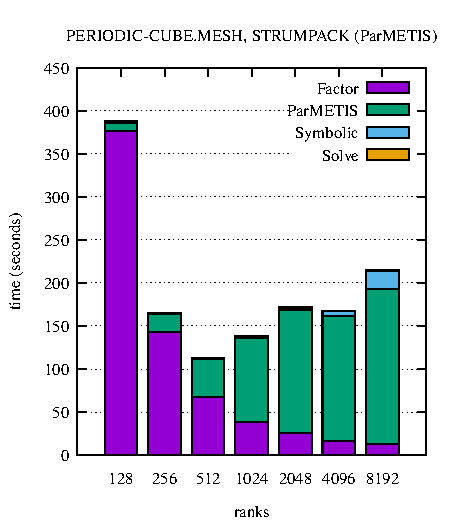
\includegraphics[scale=0.7]{projects/2.3.3-MathLibs/2.3.3.07-STRUMPACK-SuperLU/periodic-cube-scaling-strumpack.pdf}
\caption{STRUMPACK scaling with ParMETIS.}
\label{fig:strumpack-parmetis-scaling}
\end{minipage}
\begin{minipage}[b]{0.48\columnwidth}
\centering
\includegraphics[scale=0.7]{projects/2.3.3-MathLibs/2.3.3.07-STRUMPACK-SuperLU/periodic-cube-scaling-strumpack_metis.pdf}
\caption{STRUMPACK scaling with METIS.}
\label{fig:strumpack-metis-scaling}
\end{minipage}
\end{figure}

\ignore{  %%%% from last period ....
\begin{enumerate}
\item We developed and evaluated a fully algebraic sparse preconditioner in 
      STRUMPACK. On top of the baseline multifrontal direct solver, we use
      low-rank compression in dense frontal matrices to obtain approximate
      factorization. We showed that our MF+HSS preconditioner is more robust
      for numerically hard problems than many alternatives. Our code
      strong scales to over 6000 cores~\cite{ghysels2017-ipdps}
      (Fig.~\ref{fig:strumpack-scaling}).
\item We developed several strategies to enhance scalability of triangular
      solve in SuperLU\_DIST. One is an asynchronous tree-based 
      broadcast/reduction scheme which reduces latency and improves
      communication load balance. Another is efficient threading implementation
      and BLAS operations. The new code is 4.4x and 6.1x faster on 4096 cores
      with one and 50 right-hand sides, respectively~\cite{LiuTriSolve2018}
      (Fig.~\ref{fig:superlu-trisolve}).
\item We developed a new communication-avoiding 3D sparse LU factorization
      (IPDPS) algorithm that has provably asymptotic lower communication
      complexity in both latency and volume. The prototype implementation
      in SuperLU\_DIST achieves up to 27x improvement over the baseline 
      2D algorithm when run on 24,000 cores of Edison at
      NERSC~\cite{sao2018}.
\item In collaboration with ExaGraph ECP project, we evaluated the performance
      of a parallel pre-ordering algorithm called Approximate-Weight Perfect
      Matching (AWPM) for pivot selection in SuperLU\_DIST. 
      For most practical problems (e.g.,DOE apps, and SuiteSparse) the 
      weights of the perfect matchings generated by AWPM often within 99\%
      of the optimum. The MPI+OpenMP implementation on Cori at NERSC scales          up to 256 nodes –-- 2500x faster than serial MC64, and up to 114x
      speedup on 256 nodes (17,408 cores) Cori-KNL~\cite{AWPM2018}.
      The interface to AWPM are already implemented in both STRUMPACK and
      SuperLU and are released.
\end{enumerate}
} %%%% ignored from last period ....


\paragraph{Next Steps} Our future efforts will focus on the following areas:
%\textit{Describe what you are working on next.}
\begin{itemize}
\item We will build detailed performance models and performance specific
  code optimizations for the ECP applications that use our solvers.
\item We will design and implement new algorithms for the GPU systems.
\end{itemize}

\ignore{  %%%% from last period ....
\begin{itemize}
\item For STRUMPACK, we will improve the performance of the HSS solve
      routine, add OpenMP and reduce communication. We will implement
      the HOLDR low-rank format.
\item For both STRUMPACK and SuperLU, we will build detailed performance
      models and performance specific code optimizations for the ECP
      applications that use our solvers.
\end{itemize}
} %%%% ignored from last period ....

%%%% FFTX sub-project
\subsubsection{\stid{3.07} Sub-project: FFTX} \label{subsubsect:fftx}

\newpage
\subsubsection{\stid{3.12} Enabling Time Integrators for Exascale Through SUNDIALS} \label{subsubsect:SUNDIALS}

\paragraph{Overview} 

This project is enhancing the SUNDIALS library of numerical software packages for integrating differential systems in time using state-of-the-art adaptive time step technologies for use on exascale systems.  Through software infrastructure developments, this project is enabling the efficient and robust SUNDIALS time integrator packages to easily interoperate with external linear and nonlinear solver packages developed for exascale computing.  In addition, this project is providing a many-vector capability so that SUNDIALS time integrators can more easily operate on data divided over heterogeneous architectures.  Lastly, this project is supporting the deployment and use of SUNDIALS packages within ECP applications, mainly through incorporation into the discretization-based Co-Design Centers, AMReX and CEED.

Efficient time integrators are essential for ECP because they are at the core of every time-dependent simulation application.  However, many applications do not use state-of-the-art methods, and if they do, they often do not yet use them fully on their systems.  For example, at the start of the ECP the astrophysics code, Nyx, used an adaptive integration package for solving individual reactions.  However, by applying a time integration package to a larger reaction system, the code is able to vectorize more of the calculations and get an accurate solution much faster.  By allowing for solvers tuned to exascale systems and vectors that are heterogeneous, SUNDIALS will be more applicable for use in multiphysics systems running on exascale platforms.



\paragraph{Key  Challenges}

Current implementations of efficient time integrators face challenges on many fronts.  First, integrators typically have treated the full physical problem with a single step size or have relied on low order operator splitting methods to couple physical processes at different time scales. While research is moving forward within the time integration community on methods for multirate systems, the software infrastructure needs to be in place to accommodate these schemes once they are developed.   Second, typical integrators operate on problem data in the form of vectors.  These operations suffer from low arithmetic intensity, and their efficiency is often memory bandwidth limited.  Lastly, implicit integrators, which are required in many exascale systems, require efficient linear and nonlinear solvers to be highly effective.  In addition, by applying integrator-dependent controls on these solvers, their efficiency can be significantly increased.  Applying these controls, however, often requires that information about the integrator and its progress be passed to the solver, and software must be designed to effectively pass that information while ensuring adequate encapsulation to provide ease of maintenance and software extension.

\paragraph{Solution Strategy}

This project includes a number of implementation activities that will prepare the SUNDIALS suite of time integrators for exascale systems. A major activity is a redesign of all linear solver interfaces and encapsulation of the nonlinear solvers within the time integrators in SUNDIALS.  The new linear solver interfaces make it much easier to interface external solver packages while maintaining the efficiency of SUNDIALS integrators. Encapsulating the nonlinear solvers reduces redundant code and allows the time integrators to better leverage common code resulting in a lower code maintenance burden within SUNDIALS.  In addition, the integrators are able to take advantage of outside nonlinear solvers.  

This project also introduced a set of optional fused vector kernels into SUNDIALS.  These kernels execute multiple vector operations at once thereby reducing the number of kernel launches in GPU environments and also reducing the number of communications required for reduction operations.  These new kernels were added to all supplied SUNDIALS vectors and are invoked through optional interfaces.

Lastly, this project is developing a many-vector capability for SUNDIALS.  Due to the tight data encapsulation within SUNDIALS, users are able to supply any vector they would like underneath the integrators.  This project will supply the infrastructure needed to make it easy to place a vector of vectors underneath the integrators.  This vector of vectors is essential for later implementation of time integrators that will advance various parts of the system with different time step sizes.  This many-vector capability will also ease the use of different programming environments as differing vectors can be instantiated on different parts of a hybrid machine. 

\paragraph{Recent Progress}

In May of 2018, SUNDIALS 4.0.0-dev was released, including new fused vector kernels in the vector API and in all supplied vectors.  Results show speedup from using these routines, especially for parallel reductions.  In September of 2018, SUNDIALS 4.0.0-dev.2 was released, including a full redesign of the nonlinear solver interfaces to the time integrators and encapsulation of the nonlinear solevrs.  Figure \ref{fig:sunorg1} shows the new organization of SUNDIALS where separate nonlinear solver interfaces are provided for Newton and fixed point nonlinear solver methods.  These interfaces are shared across all SUNDIALS integrators.  
Individual integrators have the freedom to supply specific information from the integrator that controls the solver.  In addition, the SUNDIALS team has been collaborating closely with the AMReX Co-Design Center team to 
design effective interfaces to SUNDIALS time integrators from AMReX for applications using ODE integrators,
such as for chemistry reaction systems as in Nyx, Castro, and PELE.

\begin{figure}[htb]
	\centering
	\includegraphics[width=6in]{projects/2.3.3-MathLibs/2.3.3.12-SUNDIALS-hypre/sunorg1.pdf}
	\caption{\label{fig:sunorg1}New structure of SUNDIALS showing options for the new SUNNONLINEARSOLVER classes.}
\end{figure}

\paragraph{Next Steps}

During the remainder of FY19, this project team will:
\begin{enumerate}
\item Complete a release of SUNDIALS with a new many-vector that will enable easier use of SUNDIALS on heterogeneous architectures and for multiphysics systems.
\item Complete a scalable demonstration example program that will enable performance assessments on large-scale problems and provide a testbed for new time integrators.
\item Continue to support AMReX and CEED Co-Design Centers in their use of SUNDIALS for ECP applications.
\end{enumerate}

\subsubsection{\stid{3.01} hypre} 


\paragraph{Overview} 
The {\sl hypre} software library \cite{hypre,hypre_design_impl_2006} provides high performance preconditioners and solvers for the solution of large sparse linear systems on massively parallel computers, with particular focus on algebraic multigrid solvers. One of {\sl hypre}’s unique features is the provision of a (semi)-structured interface, in addition to a traditional linear-algebra based interface. The semi-structured interface is appropriate for applications whose grids are mostly structured, but with some unstructured features. Examples include block-structured grids, composite grids in structured adaptive mesh refinement (AMR) applications, and overset grids. These interfaces give application users a more natural means for describing their linear systems, and provide access to methods such as structured multigrid solvers, which can take advantage of the additional information beyond just the matrix. Since current architecture trends are favoring regular compute patterns to achieve high performance, the ability to express structure has become much more important. The {\sl hypre} library provides both unstructured and structured multigrid solvers, which have shown excellent scalability on a variety of high performance computers, e.g Blue Gene systems (unstructured solver BoomerAMG has scaled up to 1.25 million MPI cores with a total of 4.5 million hardware threads). It is used by many ECP application teams, including ExaAM, Subsurface, ExaWind, CEED, and more. It requires a C compiler and an MPI implementation, but it also runs in an OpenMP environment. It has some GPU capabilities.
\paragraph{Key  Challenges}

While {\sl hypre}'s solvers contain much parallelism, their main focus is the solution of sparse linear systems, leading to  very large demands on memory bandwidth. In addition, the use of multiple levels, while greatly aiding convergence of the solvers, leads to decreasing systems sizes, number of operations and parallel efficiencies on coarser levels. Particularly the unstructured algebraic multigrid solver BoomerAMG\cite{HeYa2002}, which is {\sl hypre}'s most often used preconditioner, suffers from increasing communication complexities on coarser levels. Coarse grid operators are generated by multiplying three matrices leading to increasing numbers of nonzeroes per row in the resulting matrices and with it increasing numbers of neighbor processes. While BoomerAMG's solve phase mainly consists of matrix vector products and smoothing operations, which are fairly straight forward to parallelize, even on a GPU, its setup phase is highly complex, including many branches, a lot of integer operations as well as some sequential passages. Current  interpolation strategies that lead to best convergence and performance on distributed memory machines are not suitable for implementation on GPUs or similar architectures requiring extreme parallelism. There are several algorithms that are more suitable for GPUs, such as direct interpolation, which however leads to degraded convergence. It could possibly be improved using Jacobi interpolation. All these options would need to be implemented and tested on GPUs. Since {\sl hypre} is a mature product with many solvers and interdependent features, any significant changes that affect the whole library, are tedious and require much testing to ensure that the library stays backward compatible and no features are broken.

\paragraph{Solution Strategy}

Since the upcoming computer architectures are heterogeneous with accelerators, it was very important to enable {\sl hypre} for GPUs. We looked into various options, such as the use of CUDA, OpenMP 4.5, as well as RAJA and Kokkos. We limited the latter two options to the structured interface and solvers which are more natural candidates for such an approach due to their use of macros, called BoxLoops, for loops.
Since computer architectures continue to change rapidly, it is important to come up with strategies that will facilitate future porting of the software. Therefore we decided to develop a new memory model that addresses the use of different memory locations.

\paragraph{Recent Progress}

Under internal LLNL funding we pursued the following ECP-related tasks: enabling portions of several solvers for GPUs, and introducing a new memory model that is based on an abstract machine model.
We  implemented the new memory model as well as 
various GPU capabilities in {\sl hypre}. For the structured solvers, SMG and PFMG\cite{AsFa1996}, both setup and solve phase can now completely be run on GPUs, using both CUDA or OpenMP4.5, and do not require unified memory. In addition, options to use RAJA and Kokkos are available, albeit not well tested yet. 
Porting the unstructured solver, BoomerAMG turned out to be far more complex. Currently only the solve phase can be run on the GPU for select smoothers, mainly Jacobi smoothers, and requires unified memory. The setup phase can currently be performed on the CPU only.

\begin{figure}
\centering
	\includegraphics[width=5in]{projects/2.3.3-MathLibs/2.3.3.01-xSDK/COGMRES.png}
	\caption{\label{fig:cogmres} Performance of new GMRES on Vulcan at LLNL}
\end{figure}
`
Under new ECP funding, we implemented a new GMRES solver that has better communication and parallelization properties than the current one and showed improved performance on a BG/Q. 
Figure \ref{fig:cogmres} illustrates the percentage of improvement for increasing the Krylov subspace size k for a 27-point 3D diffusion problem with n x n x n grid points per core using 8192 cores, where n=10, 20, 30, 40, 50, 60. 
For most runs loop unrolling in 8 batches was used, except for `10, no', where none was used to show the effect of saving communication and for n=40, where 4 batches were used. The current implementation is restricted to the CPU, but the solver shows great potential for GPUs. The design of the new solver was a collaboration with the ExaWind team, who demonstrated excellent GPU performance in a paper submitted to Numerical Linear Algebra with Applications \cite{cogmres}. 
We have also started to introduce a new integer datatype called HYPRE$\_$BigInt. The current {\sl hypre} version requires that all integers are converted to 64 bits when solving linear systems greater than 2 billions using the unstructured solvers. The new datatype will allow to only convert variables that need to be 64 bits in that case. This will improve performance and memory usage.

\paragraph{Next Steps}

We will pursue the following tasks:

\begin{itemize}

\item We will finalize the implementation of HYPRE$\_$BigInt and make the new capability available to {\sl hypre} users. 

\item We will continue to add new GPU capabilities to {\sl hypre}. This includes converting various components that are currently running only on the CPU to be usable on the GPU using CUDA or OpenMP 4.5. We will particularly focus on some of the smoothers, e.g. polynomial smoothers, the new GMRES solver, as well as suitable setup kernels. We also plan on improving the efficiency of interfacing applications with {\sl hypre}'s solvers.
\end{itemize}
In addition, we would like to work with ECP application teams who are using {\sl hypre} or would like to use it, to achieve best performance by tuning the solvers for them and potentially implementing suitable algorithmic changes. 



\newpage
\subsubsection{\stid{3.13} FFT-ECP}\label{subsubsect:fftecp}


\paragraph{Overview}

The FFT-ECP project indends to provide a sustainable 2D and 3D Fast Fourier 
Transform (FFT) library 
for distributed-heterogeneous parallel systems as the one projected for 
the upcoming exascale computing systems. FFT-ECP will leverage
established but {\it ad hoc} 
software tools that have traditionally been part of application 
codes, but not extracted as independent, supported libraries. 
These 3D FFTs rely on third-party 1D FFTs, either from FFTW or 
from vendor libraries.

The main objective of the FFT-ECP project is to:
\begin{itemize}
\item Collect existing FFT capabilities recently made available from ECP 
      application teams (LAMMPS/fftMPI and HACC/SWFFT);
\item Assess gaps and make available as a sustainable math library;
\item Explore opportunities to build 3D FFT libraries on vendor 1D and 
      2D kernels, especially leveraging on-node concurrency from 2D and 
      batched 1D formulations;
\item Focus on capabilities for Exascale platforms;
\item Emphasize leverage of vendor capabilities and addressing vendor 
      deficiencies over creation of new and independent software stack.
\end{itemize}

This effort is 
essential to providing a new and sustainable FFT software stack that 
leverages the large investment by the broader HPC community in FFT 
software. The payoff from this effort is almost guaranteed. 

FFTs are used in many applications such as molecular dynamics, 
spectrum estimation, fast convolution and correlation, signal 
modulation and many wireless multimedia applications. The 
distributed 3D FFT is one of the most important kernels involved 
in Molecular Dynamics (MD) computations and its performance can 
affect MD scalability at large scale. MD requires to solve 3D FFTs 
of medium size ($10^6--10^8$ points). The performance of the first 
principles calculations strongly depends on the performance of the 
FFT solver that performs many FFTs of size $\approx 10^7$ points in 
a calculation that we call batched FFT. Moreover, many Poisson PDE 
type of equations arising from many engineering areas such as PLASMA 
simulation, density field, etc., need to solve FFT of size above $10^9$. 

We found that more than dozen of ECP applications use FFT in their codes.
ECP applications that require FFT-based solvers suffer from the lack of 
fast and scalable 3D FFT routines for distributed-heterogeneous parallel 
systems as the ones projected for the upcoming exascale computing systems. 
To address these needs, FFT functionalities will first be delivered 
to the LAMMPS (molecular dynamics) and HACC (Hardware Accelerated
Cosmology Code) ECP applications. 
LAMMPS and HACC use their own FFTMPI and SWFFT FFT libraries, respectively.
FFT-ECP will first provide GPU-acceleration to these libraries.
The main components in the FFT-ECP framework are illustrated in 
Figure~\ref{fig:fft-ecp-pipeline}. The first and last step address the need 
for flexible FFT API to take application specific input and output (bricks/pencils), 
including arbitrary initial decompositions. The approach that we will persue for 
this step is to start from the current FFTMPI and SWFFT implementations and 
provide effient GPU support for their main communication primitives. 

\begin{figure}[htb]
    \centering
    \includegraphics[width=0.75\textwidth]{projects/2.3.3-MathLibs/2.3.3.13-CLOVER/ffttransormations}
    \caption{\label{fig:fft-ecp-pipeline}
    An overall 3D FFT-ECP computational pipeline:~
      1) Need flexible FFT API to take application specific input and output
         (bricks/pencils/etc., shown on the left and on right);~
      2) Need efficient packing/unpacking (on a node) and MPI communication
         routines (shown in the middle);~
      3) Need efficient 1D (or 2D in some cases) FFTs on the node (shown in the middle).}
\end{figure}

\paragraph{Key  Challenges}
\begin{enumerate}
\item
\textbf{Communication costs:}
Today's machines have very complex memory hierarchies and thus data movement, 
data layout translation, and communication should be the main focus of any 
distributed FFT library that aims to improve the performance of any ECP 
application that relies on FFT. Vendors and optimized open-source libraries 
provide very well optimized and tuned FFT routines for a single node or a 
single GPU. Therefore, although any effort on optimizing FFT kernels will 
be helpful, we prefer to target an approach that uses the available existing 
kernels and adapts them to build a more general and scalable 3D FFT library.

\item
\textbf{Appplication specifics:}
ECP applications that require FFT-based solvers suffer from the lack of fast 
and scalable 3D FFT routines for distributed-heterogeneous parallel systems 
as the ones projected for the upcoming exascale computing systems. Also, ECP 
applications may not be able to use existing FFT libraries without 
application-specific adjustments and tuning. For that, one of the main key to 
succeed with such project, is not only to study and analyze the current 
existing FFT libraries but also to study ECP application needs, study their 
FFT implementation and provide them with a suitable modular high-performance 
implementation that is flexible and easy to use and integrate in their framework.

\item
\textbf{Performance portability:}
Finally, providing many application and hardware-specific versions along with 
their parameterizations and different optimization techniques will inevitably 
create a tuning challenge. We have extensive expertize and well proven track 
record in the development and use of autotuning techniques for important GPU 
kernels. The FFT-ECP software will be linked to our autotuning tools, which 
combined with our kernels designs and use of various state-of-the-art building 
blocks will provide performance portability, software interoperability, and sustainability.
\end{enumerate}

\paragraph{Solution Strategy}

\begin{enumerate}
\item
\textbf{Evolving design:}
We will leverage vendor-optimized nodal FFT libraries as well as existing 
FFT capabilities recently made available from ECP application teams.
We will start with the fftMPI and SWFFT designs. These FFT libraries
are already integrated in ECP applications and extending them to
heterogeneous parallel systems will directly benefit the applications
and provide integrated solutions. More functionalities and application
specific optimizations will be added at a second step to support other 
ECP applications. 
\item
\textbf{Focus on communications and GPU optimizations:}
FFTs are communication bound and a main phocus in FFT-ECP is on algorithmic
design to minimize communication and efficient GPU implementations. 
Communication/computation cost and memory overhead will be analyzed and developed
for different FFT variants on current and future architecture with distributed 
and heterogeneous multi-GPU nodes. 
%Optimizing data movement as well as overlaping
%data copy with the data communication is the main bottleneck of any distributed 
%memory FFT library that must be overcommed.
\item
\textbf{Co-design with ECP application teams and vendors:}
The FFT-ECP team interacts on a regular basis with the ECP application teams
and vendors. Flexible FFT API is needed to take application specific input and 
output (bricks/pencils), including arbitrary initial decompositions. 
The APIs will be synchronized with ECP applications to be flexible, e.g., 
allowing easy construction of application-specific loading from 
and storing to arbitrary tiling of a 3D domain, data transformations from 
brick-to-pencil, pencil-to-brick, and pencil-to-pencil. Local packing and 
unpacking kernels would be accelerated leveraging GPUs' high bendwidth.
% and effient GPU transposition kernels that are already available in MAGMA.
\end{enumerate}

\paragraph{Recent Progress}
The FFT-ECP team completed an evaluation and design phase for FFTs targeting distributed 
accelerated systems. This included analysis of the current performance of FFT 
libraries and a design framework for the FFT-ECP project~\cite{thsd2018ECPFFT}. 


%The milestone delivered on the following sub-tasks:
%\begin{enumerate}
%\item Evaluation and benchmarking of current/existing FFT libraries from 
%      open-source developers and vendors;
%\item Evaluation and benchmarking of the FFT code used in other ECP 
%      applications, including LAMMPS and HACC;
%\item Study the interoperability between current vendor FFT libraries and 
%      the existing FFT library used in ECP applications, particularly for 
%      use in heterogeneous nodes with many accelerators;
%\item Propose a framework design for FFT-ECP and investigation for possible 
%      integration and/or use of vendor- developed or open-source FFT codes 
%      with our 2-D and 3-D FFT-ECP framework that emphasizes multi-GPU nodes;
%\item Analysis of the communication/computation cost and memory overhead for
%      different FFT variants and provide a study of the behavior on current 
%      and future architectures with distributed and heterogeneous multi-GPU nodes.
%\end{enumerate}

\paragraph{Next Steps}

\begin{enumerate}
\item
\textbf{Q1-Q2 FY19:}
Design and implementation phase.
\item
\textbf{Q3-Q4 FY19:}
Implementation optimization and features phase.
\end{enumerate}

\subsubsection{\stid{3.13} CLOVER Sub-project PEEKS} 
\paragraph{Overview} 
The PEEKS subproject is a focused team effort to advance the capabilities of the
ECP software stack in terms of communication-avoiding Krylov solvers and
advanced preconditioning techniques featuring fine-grained parallelism.
Previously developed techniques that are available as prototype codes -- as
well as novel algorithm developments -- are turned into production-quality 
implementations and integrated into the ECP software ecosystem 
as part of the Trilinos~\footnote{\url{https://trilinos.org/}} and the  
Ginkgo~\footnote{\url{https://github.com/ginkgo-project/ginkgo}} software 
stacks. 
%With the PEEKS project focus being on algorithm development an software design 
%and leading developers of the Trilinos and Ginkgo software packages being 
%involved in the PEEKS project, a strong focus is on software interoperability 
%and software sustainability. In consequence, there exists a strong link to the 
%other ECP math libraries and the xSDK4ECP project coordinating the ECP 
%mathematical library interoperability efforts. All technology developed in 
%PEEKS is available and disseminated via the xSDK software stack.


\paragraph{Key  Challenges}
Developing preconditioned iterative solvers for the US flagship supercomputers 
deployed in ECP, we acknowledge three major challenges coming from the hardware 
architecture:
\begin{enumerate}
\item 
Fine-grained parallelism in a single node that has to be exploited efficiently 
by the iterative solver and the preconditioner.
\item
Rising communication and synchronization cost.
\item
Computational power growing much faster than memory power, resulting on 
increased pressure on the bandwidth of all cache/memory levels.
\item 
Low-precision special function units like Tensor cores that are increasingly 
adopted by hardware architectures require sophisticated numerical schemes to be 
useful for general purpose scientific computing.
\end{enumerate}

All challenges require the redesign of existing iterative solvers with respect 
to higher parallelism within all building blocks, a reduced number of 
communication and synchronization points, favoring computations over 
communication, and adopting multiprecision algorithms for efficient hardware 
utilization. 
In the last few decades, numerous efforts 
have investigated the potential of communication-avoiding (CA) and pipelined 
Krylov solvers~\cite{yamazakiipdps2014,Cornelis2018TheCC}; however, the 
implementations usually 
remained in prototype status and rarely made it into production code. 
Similarly, significant effort was put into developing new preconditioning 
techniques that allow for the efficient parallelization of the preconditioner 
setup and the preconditioner 
application~\cite{chowisc2015,anzteuropa2015,ANZT20181}. 
Again, most implementations were experimental and rarely adopted by application 
code.
Also the concept of accelerating iterative methods by using lower precision 
formats for parts of the computations or memory access was extensively 
investigated in literature~\cite{carson1,carson2,doi:10.1002/cpe.4460}, 
while production-ready implementations are still a scarce resource. 

%In the PEEKS project we address the challenge of turning prototype 
%implementations into production-ready functionality by improving robustness 
%and 
%safeguarding against numerical breakdown, developing application- and 
%architecture-specific optimizations, and integrating into ECP application 
%projects and into a sustainable and extensible mathematical software stack.

\paragraph{Solution Strategy}

The primary thrusts of the PEEKS project are:
\begin{enumerate}
    \item \textbf{Architecture-portable software design:}
	In the Ginkgo C++ software effort, we design and develop a next-generation 
	sparse linear algebra library able to run on multi- and manycore 
	architectures. The library design is guided by radically decoupling the 
	algorithm implementation from the hardware-specific kernel implementations, 
	therewith allowing for ecosystem extensibility while allowing for heavy, 
	architecture-specific kernel optimization. 
   \item \textbf{Sustainability efforts:}
	The Ginkgo software development cycle adheres the Better Scientific 
	Software (BSSw) design principles~\cite{betterscientificsoftware} that 
	ensure production-quality code by featuring unit testing, automated 
	configuration and installation, Doxygen code documentation, as well as a 
	continuous integration and continuous benchmarking 
	framework~\cite{pasc_anzt}. Ginkgo is an 
	open source effort licensed under BSD 3-clause and ships with the latest 
	version of the xSDK package (v.0.5.0). 
   \item \textbf{Pipelined and CA Krylov methods:} 
    We realize pipelined and 
	communication-avoiding Krylov methods in production-quality code, and 
	we are actively collaborating with the ECP ExaWind project to integrate 
        our new features into their application~\cite{Yamazaki-lowsynch}. 
	\item \textbf{ParILUT -- A parallel threshold ILU:}  We are spearheading 
	the manycore-parallel computation of threshold-based 
	incomplete factorization preconditioners~\cite{sisc_anzt,ipdps_anzt}. 
	\item \textbf{Adaptive precision block-Jacobi:}  We realized a 
	production-ready block-Jacobi preconditioner that reduces the runtime by 
	carefully selecting the storage format of the distinct block inverses 
	without impacting the preconditioner quality~\cite{toms_anzt}. 
   \item \textbf{Software-defined events (SDE):}  We team up with the ECP 
    Exa-PAPI project to design and realize an ecosystem for software-defined 
    events. The idea is to provide application scientists with easy access 
    to library-, domain- and solver-specific metrics via the PAPI interface. 
    This avoids cumbersome code instrumentation and library recompilation for 
    debugging algorithm behavior or identifying performance 
    bottlenecks~\cite{doi:10.1177/1094342019846287}. 
\end{enumerate}

\paragraph{Recent Progress}
\begin{enumerate}
\item 
For improving the Ginkgo software quality and performance reproducibility, we 
realized a continuous benchmarking system permanently evaluating the 
performance of central building blocks and archiving the data~\cite{pasc_anzt}. 
We 
also realized a web-based Ginkgo Performance Explorer that allows to 
interactively explore archived performance 
data~\cite{gpewebpage}.
\item
We implemented and released five variations of communication-avoiding
and pipelined Krylov solvers in the Belos Trilinos package.
\item
We demonstrated the efficient use of communication-avoiding Krylov methods in Trilinos
inside wind turbine simulations of the ECP ExaWind project~\cite{Yamazaki-lowsynch}.
\item 
We deployed ParILUT, the first production-ready manycore-parallel algorithm for 
generating threshold-based incomplete factorization preconditioner and 
demonstrated significant speedups over state-of-the-art 
algorithms~\cite{ipdps_anzt} (see Figure~\ref{fig:ParILUTperf}).
%\item
%We released a production-ready adaptive precision block-Jacobi preconditioner 
%in the Ginkgo software library. This preconditioner separates the memory 
%format 
%from the computation format, adapts the memory format to the numerical 
%properties, and reduces the runtime cost on high-end GPUs by about 20\% 
%without 
%impacting the preconditioner quality~\cite{toms_anzt}.
\end{enumerate}

\begin{figure}[htb]
	\centering
	\includegraphics[width=6in]{projects/2.3.3-MathLibs/2.3.3.13-CLOVER/parilutspeedup}
	\caption{\label{fig:ParILUTperf}Speedup of the ParILUT over conventional 
	threshold-ILU generation on different manycore architectures. Test problems 
	are taken from the Suite Sparse Matrix Collection.}
\end{figure}


\paragraph{Next Steps}


Our next efforts are:
\begin{enumerate}
	\item \textbf{Low-synchronous orthogonalization:} The success of 
	communication-avoiding Krylov methods motivates to push the synchronization 
	limits further by deploying low-synchronous orthogonalization methods.
        (Collaboration with the ExaWind team at NREL.)
	\item \textbf{Parallel incomplete factorization preconditioner 
	application:} With the advances in the parallel incomplete factorization
	preconditioner generation, the focus increasingly turns to the efficient 
	preconditioner application. We enhance the concept of sparse approximate 
	inverse approximation for incomplete factorization preconditioners, and 
	extend the scope to novel hardware architectures featuring attractive 
	performance in the low-precision regimes.
%	\item \textbf{Get-set usage of software-defined events:} Together with the 
%	Exa-PAPI team, deployed software-defined events (SDE) in the Ginkgo sparse 
%	linear algebra library. These provide the user with access to 
%	domain-specific events like, e.g., preconditioner invocations, 
%	synchronizations, precision format changes. With building blocks differing 
%	in the resource usage, we investigate the possibility of instant power and 
%%	frequency scaling for reducing the power and energy footprint.
%	\item \textbf{Graph analytics kernels:} Preconditioning techniques like 
%	block Jacobi have a strong need for efficient and low-overhead graph 
%	analytics tools identifying strongly-connected components. We deploy GPU 
%	kernels providing this functionality while introducing only negligible 
%	overhead to the preconditioner generation.
	\item \textbf{Multiprecision sparse matrix formats:} Operations with sparse 
	matrices are memory-bound on virtually all architectures. We investigate 
	how splitting the matrix int several operators stored in value-optimized 
	less complex floating point precision formats can help improving the 
	performance of ECP applications.
	\item \textbf{Polynomial preconditioners:} The communication cost of 
	numerical preconditions is high. In particular for communication-avoiding 
	pipelined Krylov methods, the synchronization necessary by standard 
	preconditioning can become a bottleneck. We will deliver a new
        polynomial preconditioner in Trilinos (Belos). We will investigate the effectiveness 
	and efficiency of polynomial preconditioners for ECP applications.
\end{enumerate}

\subsubsection{\stid{3.13}CLOVER Sub-project SLATE}\label{subsubsect:slate}

\paragraph{Overview}

The Software for Linear Algebra Targeting Exascale (SLATE)
provides fundamental dense linear algebra capabilities
to DOE and the HPC community at large.
To this end, SLATE provides
parallel Basic Linear Algebra Subprograms (BLAS), norms,
linear systems solvers, least square solvers,
singular value and eigenvalue solvers.

The ultimate objective of SLATE is to replace the
venerable Scalable Linear Algebra PACKage (ScaLAPACK) library,
which has become the industry standard for dense linear algebra operations
in distributed-memory environments.
After two decades of operation,
ScaLAPACK is past the end of its life cycle and overdue for a replacement,
as it can hardly be retrofitted to support GPUs,
which are an integral part of today's HPC hardware infrastructure.

Primarily, SLATE aims to extract the full performance potential and maximum
scalability from modern HPC machines with large numbers nodes,
large numbers of cores per node, and multiple GPUs per node.
For typical dense linear algebra workloads, this means getting close
to the theoretical roofline peak performance and scaling to the full size of
the machine.
This is accomplished in a portable manner by relying on standards
like MPI and OpenMP.

SLATE functionalities will first be delivered to the ECP applications
that most urgently require SLATE capabilities
(NWChem, GAMESS, EXAALT, QMCPACK, CANDLE, etc.)
and to other software libraries
that rely on underlying dense linear algebra services
(STRUMPACK, SuperLU, etc.).
Figure~\ref{fig:slate-architecture} shows the role of SLATE
in the ECP software stack.

While the initial objective of SLATE is to serve as a successful,
drop-in replacement for ScaLAPACK with support for GPU accelerators,
the ultimate goal of SLATE is to deliver dense linear algebra capabilities
beyond the capabilities of ScaLAPACK.
This includes new features such as communication-avoiding
algorithms and randomization algorithms, as well as the potential to
support variable size tiles and block low-rank compressed tiles.

\begin{figure}[htb]
    \centering
    \includegraphics[width=0.75\textwidth]{projects/2.3.3-MathLibs/2.3.3.13-CLOVER/SLATE-architecture.jpg}
    \caption{\label{fig:slate-architecture}
    SLATE in the ECP software stack.}
\end{figure}

\paragraph{Key  Challenges}

\begin{enumerate}

\item
\textbf{Designing from the ground up:}
The SLATE project's primary challenge stems from the need to design the package
from the ground up, as no existing software package offers
a viable path forward for efficient support of GPUs
in a distributed-memory environment.

\item
\textbf{Facing harsh hardware realities:}
SLATE is being developed in a difficult hardware environment, where virtually
all the processing power is on the GPU side.
Achieving efficiency requires aggressive offload to GPU accelerators
and careful optimization of multiple bottlenecks, including 
interconnect technology lagging behind the computing
capabilities of the GPUs.

\item
\textbf{Facing harsh software realities:}
SLATE is being developed using cutting-edge software technologies,
and relies on modern C++ features and recent extensions
to the OpenMP standard, many of which are not fully supported by compilers
and their runtime environments.
In terms of GPU acceleration, standardized solutions are still in flux.
Also, while complete parallel programming frameworks exist, at this stage
they have to be considered research prototypes.

\end{enumerate}

\paragraph{Solution Strategy}

\begin{enumerate}

\item
\textbf{Evolving design:}
Due to the inherent challenges of designing a software package
from the ground up, the SLATE project started
with a careful analysis of the existing and emerging
implementation technologies~\cite{abdelfattah2017roadmap},
and followed with a phase
of laying out the initial design~\cite{kurzak2017designing}.
Since then, the team rolls out new computational routines every quarter.
While we continue to refactor as needed to achieve high performance, the basic
design has solidified and been published~\cite{gates2019slate-design}.

\item
\textbf{Focus on GPUs:}
Efficient GPU acceleration is the primary focus of performance
engineering efforts in SLATE.
Where applicable, highly optimized vendor implementations of GPU operations
are used, such as the batched \texttt{gemm} routine.
Where necessary, custom GPU kernels are developed, as in the case of computing
matrix norms.
Care is taken to hide communication by overlapping it with GPU computations.

\item
\textbf{Community engagement:}
The SLATE team interacts on a regular basis with the OpenMP community,
represented in ECP by the SOLLVE project, and with the MPI community,
represented in ECP by the OMPI-X project and the Exascale MPI project.
The SLATE team also engages the vendor community through our contacts
at Cray, IBM, Intel, NVIDIA, AMD, and ARM.

\end{enumerate}

\paragraph{Recent Progress}

% During 2018, the SLATE team implemented parallel BLAS, parallel norms,
% linear system solvers (LU, Cholesky, Hermitian indefinite $LTL^T$),
% and least squares solvers (QR, LQ).
During 2019, the SLATE team continued to add to its suite:
mixed-precision linear solvers for LU and Cholesky in March,
matrix inversion for LU and Cholesky in June,
and Hermitian eigenvalue and singular value solvers in September.
Routines are available in the four standard precisions (single, double,
complex-single, complex-double).
% We also continued to implement performance improvements, such as a CPU--GPU
% coherency protocol inspired by the MOSI cache consistency protocol, and
% improved handling of row-major matrices for efficient row-swapping in LU.
In addition to SLATE's native C++ API, compatibility APIs for LAPACK
and ScaLAPACK users are also provided, so that SLATE can serve
as a drop-in replacement.
All developments are documented in SLATE Working Notes
\footnote{\url{http://www.icl.utk.edu/publications/series/swans}.}


\paragraph{Next Steps}

\begin{enumerate}

\item
\textbf{Users' Guide and Developers' Guide:}
These guides will supplement SLATE's online Doxygen documentation by thoroughly
explaining both SLATE's public interface---how to integrate it into an
application, with examples---as well as SLATE's internal design, to help
new developers and outside collaborators understand the codebase. As living
documents, they will be continually updated as SLATE matures.

\item
\textbf{Band solvers:}
To SLATE's existing general band LU solvers,
we are adding Hermitian band Cholesky factorization and solve,
along with Hermitian band BLAS and norm routines.

\item
\textbf{Performance improvements:}
We have observed several routines that are not performing as well as expected.
In some cases, such as in QR, LQ, and parallel norms, we have already identified
improvements to be made to the algorithm, such as refactoring loops to improve
parallelism. In other cases, we are analyzing traces to identify and
correct problems.

\item
\textbf{Generalized Hermitian eigenvalue solver:}
We will extend SLATE's Hermitian eigenvalue solver to
handle generalized Hermitian-definite eigenvalue problems, of the form
$Ax = \lambda Bx$, $ABx = \lambda x$, or $BAx = \lambda x$.
These are of strong interest in mechanics and chemistry applications,
among others.

\item
\textbf{New C++, C, and Fortran application programming interfaces (APIs):}
The BLAS and (Sca)LAPACK APIs have served well over the past 40 years, but are
rooted in out-dated FORTRAN 77 limitations such as cryptic 5--6 letter
abbreviations (e.g., \texttt{dgemm, dgesv}). For SLATE, we will design a new,
user-friendly C++ interface (e.g., \texttt{multiply, solve}, respectively). New
C and Fortran APIs will also give better direct access to SLATE's features and
Matrix objects, without requiring use of our ScaLAPACK compatibility interface.

\item
\textbf{Non-symmetric eigenvalue problem:}
Computing the non-symmetric eigenvalue problem is significantly more
computationally expensive than the Hermitian eigenvalue problem. Our
implementation will leverage the latest advances, such as aggressive early
deflation, to achieve high performance.

\end{enumerate}

\newpage
\subsubsection{\stid{3.14} ALExa}


\paragraph{Overview}

The ALExa project ({\sl Accelerated Libraries for Exascale}) focuses on
preparing the DTK, Tasmanian and ForTrilinos libraries for exascale platforms and
integrating these libraries into ECP applications.  These libraries deliver
capabilities identified as needs of ECP applications: (1) the ability to
transfer computed solutions between grids with differing layouts on parallel
accelerated architectures, enabling multiphysics projects to seamlessly
combine results from different computational grids to perform their required
simulations (DTK);
%
(2) the ability to construct fast and memory efficient surrogates to large
scale engineering models with multiple inputs and large number of outputs,
enabling uncertainty quantification (both forward and inverse) as well as
optimization and efficient multi-physics simulations in projects such as
ExaStar (Tasmanian); and
%
(3) the ability to interface large and complex Fortran-based codes to the
growing collection of Trilinos advanced solver capabilities that can
utilize next-generation platforms, the interface is done without C/C++
interface code.

These capabilities are being developed through ongoing interactions with our
ECP application project collaborators to ensure they will satisfy requirements
of these customers.  The libraries in turn take advantage of other ECP/SW
capabilities currently in development, including Trilinos and ForTrilinos,
Kokkos and SLATE.  The final outcome of the ECP project will be a set of
libraries deployed to facilities and also made broadly available as part of
the xSDK4ECP project.


{\bf DTK} (Data Transfer Kit)

{\it Purpose:} Transfers computed solutions between grids with differing
layouts on parallel accelerated architectures.

{\it Significance:} Coupled applications frequently have different grids with
different parallel distributions; DTK is able to transfer solution values
between these grids efficiently and accurately.

{\it Mesh and mesh-free interpolation capabilities:} multivariate data
interpolation between point clouds and grids; compactly supported radial basis
functions; nearest-neighbor and moving least square implementations; support
for standard finite-element shape functions and user-defined interpolants;
common applications include conjugate heat transfer, fluid structure
interaction, and mesh deformation.

{\it Performance portable search capabilities:} shared memory and GPU
implementations of spatial tree construction; shared memory and GPU
implementations of various spatial tree queries; MPI front-end for
coordinating distributed spatial searches between sets of geometric objects
with different decompositions; communication plan generation based on spatial
search results.

{\it URL:} https://github.com/ORNL-CEES/DataTransferKit


{\bf Tasmanian} (Toolkit for Adaptive Stochastic Modeling and Non-Intrusive
Approximation)

{\it Purpose:} Constructs efficient surrogate models for high dimensional
problems and performs parameter calibration and optimization geared towards
applications in uncertainty quantification (UQ).

{\it Significance:} UQ pertains to the statistical properties of the output
from a complex model with respect to variability in multiple model inputs;
large number of simulations are required to compute reliable statistics which
is prohibitive when dealing with computationally expensive engineering
models. A surrogate model is constructed from a moderate set of simulations
using carefully chosen input values; analysis can then be performed on the
efficient surrogate.

{\it Sparse grids capabilities:} surrogate modeling and design of experiments
(adaptive multi-dimensional interpolation); reduced (lossy) representation of
tabulated scientific data; high dimensional numerical quadrature; data mining
and manifold learning.

{\it DiffeRential Evolution Adaptive Metropolis (DREAM) capabilities:}
Bayesian inference; parameter estimation/calibration; model validation.
global optimization and optimization under uncertainty.

{\it URL:} http://tasmanian.ornl.gov


{\bf ForTrilinos} (Fortran for Trilinos)

{\it Purpose:} ForTrilinos provides a seamless pathway for large and complex
Fortran-based codes to access Trilinos without C/C++ interface code.
This access includes Fortran versions of Kokkos abstractions for code
execution and data management..

{\it Significance:} The Exascale Computing Project (ECP) requires the successful
transformation and porting of many Fortran application codes in preparation for
ECP platforms. A significant number of these codes rely upon the scalable
solution of linear and nonlinear equations. The Trilinos Project contains
a large and growing collection of solver capabilities that can utilize
next-generation platforms, in particular scalable multicore, manycore,
accelerator and heterogeneous systems. Trilinos is primarily written in C++,
including its user interfaces. While C++ is advantageous for gaining access to
the latest programming environments, it limits Trilinos usage via Fortran.

{\it SWIG capabilities:}  an interface generator, SWIG, which the project is
extending, to create the object-oriented Fotran wrapper code that users can
access directly. This language translation will occur in both directions;
ForTrilinos will provide an inversion of control functionality that enables
custom extensions of the Trilinos solvers that are Fortran-based. Once the
ForTrilinos project is complete, a functional, extensible suite of capabilities
to access Trilinos on next-generation computing systems will be provided.

{\it URL:} https://github.com/trilinos/ForTrilinos

\paragraph{Key Challenges}

\indent

{\bf DTK:} General data transfer between grids of unrelated applications
requires many-to-many communication which is increasingly challenging as
communication to computation ratios are decreasing on successive HPC systems.
Search procedures to locate neighboring points and mesh cells require tree
search methods difficult to optimize on modern accelerated architectures due
to vector lane or thread divergence. Maintaining high accuracy for the
transfer requires careful attention to the mathematical properties of the
interpolation methods and is highly application-specific.

{\bf Tasmanian:} Complex models usually have significant variability in
execution time for different model inputs, which leads to massive down-time
when employing the standard fork-join adaptive sparse grid algorithms.  After
the surrogate has been constructed, collecting the samples for statistical
analysis (or multi-physics simulations) requires a massive number of basis
evaluations and many sparse and dense linear operations.

{\bf ForTrilinos:} Developing the interfaces to the C++ libraries that provide
access to cutting-edge research, such as Trilinos,  is of significant benefit
to Fortran community. However, such interfaces must be well documented,
sustainable and extensible, which would require significant amount of resources
and investment. This is further complicated by the requirements to support
heterogeneous platforms (e.g., GPUs) and inversion-of-control functionality.
The manual approach to such interfaces has been shown to be unsustainable as it
requires interface developers to have in-depth expertise in  multiple languages
and the peculiarities in their interaction on top of the time commitment to
update the interfaces with changes in the library.

\paragraph{Solution Strategy}

\nobreak


\indent

{\bf DTK:} State-of-the-art, mathematically rigorous methods are used in DTK
to preserve accuracy of interpolated solutions.  Algorithms are implemented in
a C++ code base with extensive unit testing on multiple platforms.  Trilinos
packages are used to support interpolation methods.  Kokkos is used to achieve
performance portability across accelerated platforms.

{\bf Tasmanian:} Implement asynchronous DAG-based sparse grids construction
methods that preserve the convergence properties of the fork-join algorithms
but are insensitive to fluctuations in model simulation time.  Port the basis
evaluations and linear algebra to the GPU accelerators, and leverage the
SLATE/MAGMA capabilities to ensure performance portability across relevant
platforms.

{\bf ForTrilinos:} Develop a Fortran module for the Simplified Wrapper
Interface Generator (SWIG) utility~\cite{beazley1996swig}. SWIG is used to parse
C++ code and generate wrapper code, and was already used for this purpose for
several dozen target languages, most notably Python. The project took the
approach of adding a Fortran 2003 wrapper generator for SWIG in order to
fulfill many of the critical feature requirements for ForTrilinos.
The developed SWIG/Fortran functionality allowed to proceed with automatic
generation of Fortran interfaces to selected Trilinos libraries. The work is
conducted in phases, with each phase increasing the number of wrapped of
Trilinos packages.

%----------------------------------------

\paragraph{Recent Progress}

\indent

{\bf DTK:} Extensive optimization work has yielded significant performance
improvements on accelerated and heterogeneous architectures. Work with partner
application ExaAM (WBS 2.2.1.05) created a preliminary multiphysics driver
capability for additive manufacturing simulations.

\begin{figure}[htb]
        \centering
        \includegraphics[width=3.0in]{projects/2.3.3-MathLibs/2.3.3.14-ALExa-ForTrilinos/dtk-gpu}
        \caption{\label{fig:dtk-gpu}DTK search performance relative to Boost with Intel Xeon E5-2698 and Nvidia P100. 10M points randomly distributed in a unit cube, 1M queries. The time is in seconds. Speedup in bold.}
\end{figure}

{\bf Tasmanian:} The infrastructure of Tasmanian has been upgraded to support
the broader ECP focus of the work.  GPU acceleration of sparse grid surrogates
has been implemented.  Tasmanian recently enabled the ExaStar project to
reduce the size of a large-memory table of neutrino opacities by 10X while
still preserving accuracy.

\begin{figure}[htb]
        \centering
        \includegraphics[width=1.5in]{projects/2.3.3-MathLibs/2.3.3.14-ALExa-ForTrilinos/tasmanian-gpu}
        \caption{\label{fig:tasmanian-gpu}Tasmanian approximation (right) of neutrino capacities (left).}
\end{figure}

{\bf ForTrilinos:}
Figure~\ref{fig:fortran_ioc} illustrates a new Inversion-of-Control~(IoC)
implementation in ForTrilinos. The new approach allows Fortran users to define
an operator by using a derived type on the Fortran side, and use Trilinos
algorithms, e.g. Krylov solvers, to solve the linear system with that operator.

\begin{figure}[htb]
    \centering
    \includegraphics[scale=0.8,width=6in]{projects/2.3.3-MathLibs/2.3.3.14-ALExa-ForTrilinos/ForTrilinos_ioc}
    \caption{\label{fig:fortran_ioc}The proposed Inversion-of-Control approach
    allowing Fortran applications to define operators on Fortran side while
    still using ForTrilinos types.}
\end{figure}

This approach allows the user callback functions to interact with native Fortran
types and ForTrilinos class wrapper types. In the same vein, users would not
have to manually pass \texttt{type(C\_PTR)} instances into and out of the
callback function, as the C++ Fortran conversions can be tedious and
error-prone, which indeed is the motivation for using SWIG to generate
ForTrilinos.  Another important feature is that it allows the application code
to extend Trilinos without having to generate any new interface code, either by
hand or using SWIG. In other words, the Fortran end user should not have to know
C++ or SWIG.

%----------------------------------------

\paragraph{Next Steps}

\indent

{\bf DTK:} DTK search and communication capabilities will deployed in a new,
lightweight library, ArborX, to provide these ECP investments to a broader
user base.

{\bf Tasmanian:} Work will continue with the development of mixed precision
algorithms for fast surrogate evaluations and integratinv the capability within
the ExaStar project.

{\bf ForTrilinos:} the next efforts will include
\begin{enumerate}
  \item \textbf{Provide wrappers for more libraries:} ForTrilinos will continue
    efforts to increase the number of wrapped Trilinos libraries. The scheduled
    release of the next phase of the project will include libraries
    corresponding to nonlinear solvers, such as NOX.
  \item \textbf{Integrate developed capabilities into applications:} E3SM-MMF
    is an Earth system model development and simulation project. It relies on
    Trilinos for its implicit capabilities. The ForTrilinos project will
    integrate the developed nonlinear solver with IoC into E3SM-MMF to provide
    path forward to heterogeneous stack.
  \item \textbf{Provide interfaces for heterogeneous platforms:} ForTrilinos
    will develop support for heterogeneous memory through providing access to
    Kokkos-based interfaces in Trilinos. This will allow full exposure to
    Trilinos capabilities targeting Exascale machines.
\end{enumerate}

%----------------------------------------

% \subsubsection{\stid{3.14} ForTrilinos}

\paragraph{Overview}

The Exascale Computing Project (ECP) requires the successful transformation and porting of many Fortran application codes in preparation for ECP platforms. A significant number of these codes rely upon the scalable solution of linear and nonlinear equations. The Trilinos Project contains a large and growing collection of solver capabilities that can utilize next-generation platforms, in particular scalable multicore, manycore, accelerator and heterogeneous systems. Trilinos is primarily written in C++, including its user interfaces. While C++ is advantageous for gaining access to the latest programming environments, it limits Trilinos usage via Fortran. Several ad hoc translation interfaces exist to enable Fortran usage of Trilinos, but none of these interfaces is general-purpose or written for reusable and sustainable external use.

ForTrilinos provides a seamless pathway for large and complex Fortran-based
codes to access Trilinos without C/C++ interface code. This access includes
Fortran versions of Kokkos abstractions for code execution and data management.
The project uses an interface generator, SWIG, which the project is extending,
to create the object-oriented Fortran wrapper code that users can access directly. This language translation will occur in both directions; ForTrilinos will provide an inversion of control functionality that enables custom extensions of the Trilinos solvers that are Fortran-based. Once the ForTrilinos project is complete, a functional, extensible suite of capabilities to access Trilinos on next-generation computing systems will be provided. Several examples of this technology will be demonstrated within ECP codes with the aim of meeting their simulation goals and illustrate the technology to other Fortran-based ECP codes. As a second benefit to ECP from this effort, the ForTrilinos approach of using SWIG to generate interfaces could be extended to other C/C++ based tools and software within the ECP stable.

\paragraph{Key Challenges}

Developing the interfaces to the C++ libraries that provide access to cutting-edge research, such as Trilinos,  is of significant benefit to Fortran community. However, such interfaces must be well documented, sustainable and extensible, which would require significant amount of resources and investment. This is further complicated by the requirements to support heterogeneous platforms (e.g., GPUs) and inversion-of-control functionality. The manual approach to such interfaces has been shown to be unsustainable as it requires interface developers to have in-depth expertise in  multiple languages and the peculiarities in their interaction on top of the time commitment to update the interfaces with changes in the library.

ForTrilinos addresses both the issue of reducing interface generation cost through investment in tool configuration and usage to make the process as automatic as possible, and the issue of providing the full-featured interface to Trilinos library, including access to manycore, accelerator and heterogeneous solver capabilities in Trilinos.

\paragraph{Solution Strategy}

The ForTrilinos project has two primary thrusts:
\begin{enumerate}
  \item \textbf{SWIG development to support Fortran wrapping:} The new Fortran
    module for SWIG allows for automatic generation of interfaces.
  \item \textbf{Incremental wrapping of selected Trilinos functionality:}
    ForTrilinos provides robust interfaces to selected Trilinos capabilities,
    including distributed data objects, linear and nonlinear solvers.
\end{enumerate}

ForTrilinos started with developing a Fortran module for the Simplified Wrapper Interface Generator (SWIG) utility~\cite{beazley1996swig}. SWIG is used to parse C++ code and generate wrapper code, and was already used for this purpose for several dozen target languages, most notably Python. The project took the approach of adding a Fortran 2003 wrapper generator for SWIG in order to fulfill many of the critical feature requirements for ForTrilinos.

The developed SWIG/Fortran functionality allowed to proceed with automatic generation of Fortran interfaces to selected Trilinos libraries. The work is conducted in phases, with each phase increasing the number of wrapped of Trilinos packages.

The first phase, completed in the first year, developed interfaces for a critical set of features required for solving linear and eigen-problems. The second phase addresses nonlinear solver, including developing automatic approach for inversion-of-control capability. Finally, in the third phase, the challenge of interoperable heterogeneous data passing between Fortran and C++, including GPU data, is addressed, including performance testing.

\paragraph{Recent Progress}

Figure~\ref{fig:fortran_ioc} illustrates a new Inversion-of-Control~(IoC)
implementation in ForTrilinos. The new approach allows Fortran users to define
an operator by using a derived type on the Fortran side, and use Trilinos
algorithms, e.g. Krylov solvers, to solve the linear system with that operator.

\begin{figure}[htb]
    \centering
    \includegraphics[scale=0.8,width=6in]{projects/2.3.3-MathLibs/2.3.3.14-ALExa-ForTrilinos/ForTrilinos_ioc}
    \caption{\label{fig:fortran_ioc}The proposed Inversion-of-Control approach
    allowing Fortran applications to define operators on Fortran side while
    still using ForTrilinos types.}
\end{figure}

This approach allows the user callback functions to interact with native Fortran
types and ForTrilinos class wrapper types. In the same vein, users would not
have to manually pass \texttt{type(C\_PTR)} instances into and out of the
callback function, as the C++ Fortran conversions can be tedious and
error-prone, which indeed is the motivation for using SWIG to generate
ForTrilinos.  Another important feature is that it allows the application code
to extend Trilinos without having to generate any new interface code, either by
hand or using SWIG. In other words, the Fortran end user should not have to know
C++ or SWIG.

\paragraph{Next Steps}

Our next efforts include:
\begin{enumerate}
  \item \textbf{Provide wrappers for more libraries:} ForTrilinos will continue
    efforts to increase the number of wrapped Trilinos libraries. The scheduled
    release of the next phase of the project will include libraries
    corresponding to nonlinear solvers, such as NOX.
  \item \textbf{Integrate developed capabilities into applications:} E3SM-MMF
    is an Earth system model development and simulation project. It relies on
    Trilinos for its implicit capabilities. The ForTrilinos project will
    integrate the developed nonlinear solver with IoC into E3SM-MMF to provide
    path forward to heterogeneous stack.
  \item \textbf{Provide interfaces for heterogeneous platforms:} ForTrilinos
    will develop support for heterogeneous memory through providing access to
    Kokkos-based interfaces in Trilinos. This will allow full exposure to
    Trilinos capabilities targeting Exascale machines.
\end{enumerate}
 % merged with ALExa
\newpage


\subsection{\dataviz}
This section present projects in \dataviz.
\newpage
\subsubsection{\stid{4.01} \dataviz\ Software Development Kits} 

\paragraph{Overview} 
The \dataviz\ SDK effort is focused on identifying meaningful aggregations of products in this technical area.  SDK efforts are in the early stages of planning and execution.  Most of the work on SDKs has been driven from the \ecosystem\ technical area.  A description of the SDK effort can be found in Section~\ref{subsubsect:ecosystem-sdk}.

\newpage
\subsubsection{\stid{4.09} ADIOS} 
\paragraph{Overview} 
The Adaptable I/O Systems, ADIOS~\cite{liu2014hello}, is designed to tackle I/O and data management challenges posed  by  large-scale computational science applications running on DOE computational resources. ADIOS has  dramatically  improved  the I/O performance of Petascale  applications from a   wide range of science disciplines, thereby enabling them to accomplish their missions. The ADIOS ECP project is working on goal of transforming the ADIOS 1.x version, which has been used successfully on Petascale resources into a tool that will efficiently utilize  the underlying Exascale hardware, and create a   community I/O framework that can allow different ECP software to be easily  “plugged” into the framework. The cornerstone of this project are to 1) efficiently  address Exascale technology changes in compute, memory, and interconnect for Exascale applications; 2) develop  a  production-quality data staging method to support Exascale applications and software  technologies that require flexible in situ data reduction and management capabilities; and 3) use state  of the  art software engineering methodologies to    make it   easier for the DOE community to    use, maintain, and extend ADIOS. More precisely, our aim is to    develop and deploy a   sustainable and extensible software ecosystem. To make this into an ecosystem (rather than a point solution),this effort must result in  an  infrastructure than can be used effectively, customized, and shared among a   variety of users, Exascale applications, and hardware technologies. Technically, we are achieving  this goal  by: refactoring ADIOS  with the  goal  of improving modularity, flexibility, and extensibility by using C++; and extending, tuning, and hardening core services, such as I/O and staging that supports Exascale applications, architectures, and technologies.

\paragraph{Key  Challenges}
The core challenge of ADIOS is in its name -- adaptability.  In order to present a uniform user interface while also being able to harness the performance improvements available in the wide variety of storage and interconnect capabilities, the internal structure of the ADIOS framework must address a number of portability, functionality, and performance tuning challenges.  The internals should be constructed so that with no more than a small flag or runtime configuration a science code can move from doing I/O into a large Lustre parallel file system (with automatic calculation of file striping and number of files per directory) to utilizing burst buffer storage (with controls for delayed synchronization between the buffer and an archival store) or feeding the data directly into a concurrent application   

The challenge of supporting hardware portability and runtime performance tuning also impose a third related challenge for software engineering of the system.  In order for the code to be sustainable in the long term, while also offering guarantees of service to the end user, requires special attention to the architecture of the code base.  The consequences of trying to address these three challenges, hardware portability, runtime performance, and sustainable engineering, have driven our approach and deliverable schedule for ADIOS in ECP.

\paragraph{Solution Strategy}

The ADIOS effort has two primary thrusts:
\begin{enumerate}
	\item \textbf{Scalable I/O:} ADIOS has a data format designed for large scale parallel I/O and has data transport solutions to write/read data from/to the storage system(s) efficiently.
	\item \textbf{Scalable data staging support:}  ADIOS includes data transport solutions to work on data in transit, that is, to move data memory-to-memory, from one application stage to another without using file system I/O.
\end{enumerate}

The challenges of portability and performance apply for both of these thrusts; to a certain extent, the third challenge around software engineering emerges from the need to support these two very different categories under a single user interface.  Capitalizing on the experiences and performance expertise from our initial ADIOS platform, the ECP project wraps and extends this functionality to make it more sustainable, maintainable, and hopefully also more approachable for a wide community of users and developers.  The project approach focuses on doing deep dives with end scientist users and developers in order to make sure that the computer science development process leads to specific, verifiable results that impact the customers.


\paragraph{Recent Progress}

A new version of the Application Programming Interface unifies staging I/O and file I/O~\cite{ADIOS2-docs}, and the new, object-oriented, code framework~\cite{ADIOS2-git} supports  writing and reading files in two different file formats (ADIOS BP format and HDF5 format) and in situ with different staging implementations for various use cases. The new framework focuses on sustainable development and code reusability. The team also created the new scalable staging transport learning from the many lessons from using ADIOS for data staging and code coupling by applications in the past. As can be seen in Figure~\ref{fig:adios-example}, this past experience with methods and deep science engagements has led to demonstrations at leadership computing scale (on Titan and Summit).

\begin{figure*}[!th]
	\begin{center}
		\includegraphics[width=0.75\textwidth]{projects/2.3.4-DataViz/2.3.4.09-ADIOS/ADIOS_in_ECP.png}
		\caption{An example of using ADIOS to support ECP science.  This sketch represents the demonstration at the February 2018 ECP Meeting, which featured WDM Fusion, CODAR, ADIOS, and other joint ECP activities.  Note that all of the green arrows in the figure represent data communication or storage handled by the ADIOS infrastructure.}
		\label{fig:adios-example}
	\end{center}
\end{figure*}

The new design focuses on stability and scalability so that applications can rely on it in daily production runs just as they have relied on the high performance file I/O of ADIOS. The new code base is governed with state-of-the art software development practices, including GitHub workflow of Pull-Requests with reviews, continuous integration that enforces well-tested changes to the code only, and nightly builds to catch errors on various combinations of architecture and software stack as soon as possible. Static and dynamic analysis are integrated to the GitHub workflow to catch errors before they cause trouble. Code coverage tools also help with increasing code quality. The team has access to and the code is continuously tested on DOE machines (Summit, Cori and Theta) using several ECP application codes and realistic science simulation setups (e.g. for WDMApp, E3SM-MMF and EXAALT application setups). 


\paragraph{Next Steps}
In the fourth year, the team has multiple goals: a) to tune ADIOS for Summit, evaluating its performance in ECP applications on this system, determine problems and improve the code base b) develop a performance testing framework that allows for experimentation with real applications and for easier collection of performance metrics,  c) to evaluate how to incorporate ADIOS technology in the HDF5 software and d) to add ADIOS to more ECP applications, specifically targeting this year the OpenPMD particle data format and library used by WarpX. 

\newpage
\subsubsection{\stid{4.10} DataLib} 

\paragraph{Overview} 

Data Libraries and Services Enabling Exascale Science (DataLib). The
DataLib project encompasses multiple related activities in user-level
storage and I/O support for ECP codes on upcoming DOE platforms,
providing a number of options for effectively storing and retrieving
data and tools for assessing I/O behavior and performance.
%
The \textbf{ROMIO} and \textbf{Parallel netCDF} (PnetCDF) activities
focus on existing standards-based interfaces in broad use, assisting
in performance debugging on new platforms and augmenting existing
implementations to support new storage models (e.g., “burst
buffers”). In addition to being used directly by applications, ROMIO
and PnetCDF are also indirectly used in HDF5 and netCDF-4. Our work is
ensuring that these libraries are ready for upcoming platforms and
effective for their users (and ready as alternatives if other
libraries fall short).
%
The \textbf{Darshan} I/O characterization toolset is an instrumentation tool
deployed at facilities to capture information on I/O behavior of
applications running at scale on production systems. It has become
popular at many DOE facilities and is usually “on by default”. Darshan
data dramatically accelerates root cause analysis of performance
problems for applications and can also (in some cases) assist in
correctness debugging. Our work in this project focuses on extending
Darshan to new interfaces and ensuring readiness on upcoming
platforms.
%
The \textbf{Mochi} and \textbf{Mercury} software tools are building blocks for
user-level distributed HPC services. They address issues of
performance, programmability, and portability in this key facet of
data service development. Mercury is being used by Intel in the
development of their DAOS storage service and in other data service
activities, while within ECP the HXHIM and UnifyCR projects also have
plans to leverage these tools. In addition to working with these
stakeholders and ensuring performance and correctness on upcoming
platforms, we are also working with ECP application teams to customize
data services for their needs (e.g., memoization, ML model management
during learning).

\paragraph{Key Challenges}

Each of these subprojects has its own set of challenges. Libraries
such as ROMIO and PnetCDF have numerous users from over a decade of
production use, yet significant changes are needed to address the
scale, heterogeneity, and latency requirements of upcoming
applications. New algorithms and methods of storing data are required.
%
For Darshan, the challenge is to operate in a transparent manner in
the face of continuing change in build environments, to grow in
functionality to cover new interfaces while remaining ``lean'' from a
resource utilization perspective, and to interoperate with other tools
that use similar methods to hook into applications.
%
Mochi and Mercury are new tools, so the challenge in the context of
these tools is to find users, adapt and improve to better support
those users, and gain a foothold in the science community.

\paragraph{Solution Strategy}

\emph{Transparently refactoring application I/O.}
Collective I/O is an important optimization in codes where phases of
I/O are naturally identifiable: individual I/O operations from
application processes are transparently refactored (i.e., without
application code changes) to achieve the same goals at lower cost. We
will improve collective I/O techniques for Exascale through tighter
integration with I/O forwarding layers, topology awareness, and
employing collective approaches in higher-level libraries where
additional information is available.

\emph{Intermediate storage and alternative data organizations.}
Nonvolatile memory (NVM) or
solid-state disk (SSD) integrated into platforms provides a pool of
fast storage where data can be stored temporarily or staged for
writing to an external store (e.g., parallel file system). Recognizing
that this data is transient, alternative organizations (e.g.,
provide higher performance.

\emph{Capturing and reconstructing I/O behavior.}
Darshan characterizes fully the POSIX and MPI-IO layers and captures
some statistics for HDF5 and PnetCDF. We will improve our coverage of
HDF5, PnetCDF, and ADIOS to better enable understanding of these
codes. We will reach out to other library teams to consider
characterization of them as well (e.g., SCR, FTI, PIO, SILO).

\emph{Mercury porting and support for relevant platforms.}
Mercury is an RPC/bulk data communication library for use in HPC
services and co-developed by the HDF Group. We will work with system
vendors to enable efficient Mercury communication on the platforms of
interest (e.g., UCX/PAMI on IBM).

\emph{Data service co-design with application teams.}
A number of candidate ECP applications have data service needs (e.g.,
material property databases, producer-consumer data pipelines,
multi-scale/physics simulation coupling, multi-modal data organization
and indexing). We will identify application teams with data service
requirements that are particularly ill-suited to solution by vendor
offerings (e.g., parallel file systems, standard burst buffers,
cloud-based databases) and co-design, develop, and evolve specialized
services based on our components to meet their specific requirements
for ECP.

\paragraph{Recent Progress}

\emph{Darshan.}
Darshan has won a 2018 R\&D 100 Award. The award is given by R\&D magazine
to the 100 top new technologies for the year. The Darshan software
package enables researchers to investigate and tune the I/O behavior of
complex high-performance computing (HPC) applications. A key feature of
the package is its ability to run on some of the largest systems in the
world, including Crays, IBM Blue Gene systems and Linux clusters. 

We've begun designing automatic tracing in Darshan (STDM12-13), starting
with an analysis of use cases provided by a number of stakeholders.


\emph{Mochi and Mercury.}
Nightly tests are now running on Aires, InfiniBand, and OmniPath networks
(STDM12-7). See below for more information on STDM12-7.

\emph{PnetCDF.}
Figure~\ref{fig:pnetcdf} illustrates a refactoring of the PnetCDF
library to include a dispatch layer. The dispatch layer provides a
mechanism for implementing multiple back-ends under the standard
API. This functionality is being used to enable writing in a log
format for intermediate data and access of data in the netCDF-4 format
(stored in HDF5 files).

The PnetCDF Burst Buffer capabilities have been tested, and results were
published at the PDSW workshop in conjunction with SC18 (STDM12-10).
ADIOS and netCDF-4 read capabilities have been implemented in PnetCDF,
and testing of ADIOS read capabilities under PnetCDF (STDM12-11) is
underway.
%
We continue to make improvements in support of E3SM workloads.

\emph{ROMIO.}
Integration of pipelined I/O functionality into ROMIO (STDM12-9) is complete,
specifically into the Lustre driver. We continue to improve the LogFS
ROMIO back-end.

\emph{ParSplice.}
Work with ParSplice is complete for now (STDM12-21). Specialized segment
store attains similar performance as a tightly integrated solution for
current problem sizes. As the application team scales up, we expect
the scalability of the segment store to provide a performance benefit,
but this is TBD.

\emph{Portage/JALI}. Examining Portage/JALI as next candidate for service
specialization (STDM12-21).

\begin{figure}[htb]
        \centering
        \includegraphics[height=2.5in]{projects/2.3.4-DataViz/2.3.4.10-DataLib/pnetcdf-figure.pdf}
        \caption{\label{fig:pnetcdf} The new PnetCDF dispatch layer provides flexibility to target different back-end formats and devices under the PnetCDF API used by many existing applications.
        }
\end{figure}

\paragraph{Next Steps}
Closing on the end of our first three year project period, we are focusing
on (a) wrapping up software releases of Darshan, PnetCDF, and Mercury
suite (STDM12-13, STDM12-11, and STDM12-12); (b) adding new optimized
collective I/O capabilities in ROMIO (STDM12-14); (c) completing automatic
triggering of tracing in Darshan (STDM12-13); and (d) investigating
additional use cases of specialized services in ECP applications
(STDM12-21). 


\newpage
\subsubsection{\stid{4.13} ECP/VTK-m}

\paragraph{Overview}
The ECP/VTK-m project is providing the core capabilities to perform scientific visualization on Exascale architectures.
The ECP/VTK-m project fills the critical feature gap of performing visualization and analysis on processors like graphics-based processors and many integrated core.
The results of this project will be delivered in tools like ParaView, VisIt, and Ascent as well as in stand-alone form.
Moreover, these projects are depending on this ECP effort to be able to make effective use of ECP architectures.

One of the biggest recent changes in high-performance computing is the increasing use of accelerators.
Accelerators contain processing cores that independently are inferior to a core in a typical CPU, but these cores are replicated and grouped such that their aggregate execution provides a very high computation rate at a much lower power.

Current and future CPU processors also require much more explicit parallelism.
Each successive version of the hardware packs more cores into each processor, and technologies like hyper threading and vector operations require even more parallel processing to leverage each core's full potential.

VTK-m is a toolkit of scientific visualization algorithms for emerging processor architectures.
VTK-m supports the fine-grained concurrency for data analysis and visualization algorithms required to drive extreme scale computing by providing abstract models for data and execution that can be applied to a variety of algorithms across many different processor architectures.

The ECP/VTK-m project is building up the VTK-m codebase with the necessary visualization algorithm implementations that run across the varied hardware platforms to be leveraged at the Exascale.
We will be working with other ECP projects, such as ALPINE, to integrate the new VTK-m code into production software to enable visualization on our HPC systems.

\paragraph{Key  Challenges}
The scientific visualization research community has been building scalable HPC algorithms for over 15 years, and today there are multiple production tools that provide excellent scalability.
However, our current visualization tools are based on a message-passing programming model.
More to the point, they rely on a coarse decomposition with ghost regions to isolate parallel execution \cite{Ahrens2001,Childs2010}.
However, this decomposition works best when each processing element has on the order of a hundred thousand to a million data cells \cite{ParaViewTutorial} and is known to break down as we approach the level of concurrency needed on modern accelerators \cite{Moreland2012:Ultravis,Moreland2013:UltraVis}.

DOE has made significant investments in HPC visualization capabilities.
For us to feasibly update this software for the upcoming Exascale machines, we need to be selective on what needs to be updated, and we need to maximize the code we can continue to use.
Regardless, there is a significant amount of software to be engineered and implemented, so we need to extend our development resources by simplifying algorithm implementation and providing performance portability across current and future devices.


\paragraph{Solution Strategy}
The ECP/VTK-m project leverages VTK-m \cite{Moreland2016:VTKm} to overcome these key challenges.
VTK-m has a software framework that provides the following critical features.

\begin{enumerate}
\item \textbf{Visualization building blocks:}
  VTK-m contains the common data structures and operations required for scientific visualization.
  This base framework simplifies the development of visualization algorithms \cite{VTKmUsersGuide}.
\item \textbf{Device portability:}
  VTK-m uses the notion of an abstract device adapter, which allows algorithms written once in VTK-m to run well on many computing architectures.
  The device adapter is constructed from a small but versatile set of data parallel primitives, which can be optimized for each platform \cite{Blelloch1990}.
  It has been shown that this approach not only simplifies parallel implementations, but also allows them to work well across many platforms \cite{Lo2012,Larsen2015,Moreland2015}.
\item \textbf{Flexible integration:}
  VTK-m is designed to integrate well with other software.
  This is achieved with flexible data models to capture the structure of applications' data \cite{Meredith2012} and array wrappers that can adapt to target memory layouts \cite{Moreland2012:PDAC}.
\end{enumerate}

Even with these features provided by VTK-m, we have a lot of work ahead of us to be ready for Exascale.
Our approach is to incrementally add features to VTK-m and expose them in tools like ParaView and VisIt.


\begin{figure}[t]
  \centering
  \includegraphics[width=2in]{projects/2.3.4-DataViz/2.3.4.13-ECP-VTK-m/VTKm-Multiblock}\quad
  \includegraphics[width=2in]{projects/2.3.4-DataViz/2.3.4.13-ECP-VTK-m/VTKm-Gradients}\quad
  \includegraphics[width=2in]{projects/2.3.4-DataViz/2.3.4.13-ECP-VTK-m/VTKm-FieldToColors}
  \caption{
    Examples of recent progress in VTK-m include (from left to right) multiblock data structures, gradient estimation, and mapping of fields to colors.
  }
  \label{fig:VTKmRecent}
\end{figure}

\paragraph{Recent Progress}
The VTK-m project is organized into many implementation activities.
The following features have been completed in the FY18 fiscal year.

\begin{itemize}
\item \textbf{Multiblock Data:}
  Treat multiple blocks of data, such as those depicted in Figure \ref{fig:VTKmRecent} at left, as first-class data sets.
  %Direct support of multiblock data not only provides programming convenience but also allows us to improve scheduling tasks for smaller groups of data.
\item \textbf{Gradients:}
  Gradients, depicted in Figure \ref{fig:VTKmRecent} at center, are an important metric of fields and must often be derived using topological data.
  %Gradients are also fundamental in finding important vector field qualities like divergence, vorticity, and q-criterion.
\item \textbf{Field to Colors:}
  Pseudocoloring, demonstrated in Figure \ref{fig:VTKmRecent} at right, is a fundamental feature of scientific visualization, and it depends on a good mechanism of converting field data to colors.
\item \textbf{VTK-m 1.1 Release:}
  VTK-m 1.1 was released in December 2017.
\item \textbf{Extract External Surface:}
  When rendering solid objects, it is only necessary to render the external surface of the object as the interior of the volume is hidden \cite{Lessley2016,Lessley2017}.
  %As such, external surface extraction is one of the most common operations in scientific visualization applications.
\item \textbf{Coordinate system transformations:}
  3D rendering systems operate in Cartesian coordinate systems.
  However, data are sometimes referenced in cylindrical or spherical coordinate systems.% to match the physical structure of the data.
  %Consequently, visualization tools need a fast method to convert coordinates among different spaces.
\item \textbf{Affine Transformations:}
  Affine transformations, which include translate, rotate, and scale, are a common and important method to manipulate objects in 3D space.
\item \textbf{Location Structures:}
  Finding mesh components from a coordinate in space requires search structures.
\item \textbf{Rendering Topological Entities:}
  It is often helpful to analysts to view representations of the constitute components of a mesh.
\item \textbf{OpenMP:}
  %Much of the code we wish to integrate with uses OpenMP \cite{OpenMP}, which can conflict with other threading implementations.
  %VTK-m now supports multiple threading libraries, including OpenMP, to better match the code it integrates with.
  VTK-m now supports OpenMP \cite{OpenMP} to better match the code it integrates with.
\end{itemize}

\paragraph{Next Steps}
Our next efforts include:

\begin{itemize}
\item \textbf{Dynamic Types:}
  %The initial implementation of VTK-m used templating to adjust to different data structures.
  %However, when data types are not known at compile time, which is common in applications like ParaView and VisIt, templating for all possible combinations becomes infeasible.
  Provide mechanisms to enable runtime polymorphism.
\item \textbf{ZFP:}
  We are assisting the ZFP project (WBS 2.3.4.11) by helping them implement {\zfp} in VTK-m and port across ECP platforms.
\item \textbf{Clip:}
  Cuts away a mesh based on a spatial intersection or field values.
\item \textbf{Ghost Cells:}
  Provide better support for ghost/halo regions across blocks in a mesh.
\item \textbf{Merge Points:}
  Combine points in a mesh that can be considered coincident.
\item \textbf{Connected Components:}
  Identify regions in a mesh where all cells are topologically connected to each other.
\item \textbf{Particle Advection:}
  Many flow visualization algorithms depend on computing the movement of weightless particles in a flow vector field.
%% \item \textbf{Lightweight Cell Library:}
%%   There is much repetition between VTK-m and other visualization code to perform operations on cells.
%%   We would like to consolidate that code into a lightweight library.
\end{itemize}

\noindent
{\tiny Sandia National Laboratories is a multimission laboratory managed and operated by National Technology \& Engineering Solutions of Sandia, LLC, a wholly owned subsidiary of Honeywell International Inc., for the U.S. Department of Energy's National Nuclear Security Administration under contract DE-NA0003525. \hfill SAND~2018-13745~R
\par}

\newpage
\subsubsection{\stid{4.14} VeloC: Very Low Overhead Checkpointing System} 

\paragraph{Overview} 

The VeloC-SZ project aims to provide VeloC, a high-performance, scalable
checkpoint/restart framework that leverages multi-level checkpointing
(the combination of several resilience strategies and heterogeneous
storage) to ensure that ECP applications run to completion with
minimal performance overhead. It delivers a production-ready solution
that increases development productivity by reducing the complexity of
having to deal with a heterogeneous storage stack and multiple vendor
APIs. VeloC offers a client library that can be used by the
applications to capture local application states, which are then
coordinated and persisted using a resilience engine.  VeloC runs the resilience engine asynchronously, which overlaps a large part of the checkpointing
with the application runtime, thereby reducing its overhead.

VeloC has been released and shows significant lower checkpointing
overhead for several ECP applications, such as HACC, LatticeQCD, 
EXAALT. VeloC is a next generation checkpointing system that builds on SCR, which won the prestigious R\&D 100 award in 2019. 

\paragraph{Key Challenges}
VeloC faces several key challenges:
\begin{itemize}
    \item \textbf{I/O bottlenecks:} applications typically employ simple checkpoint-restart mechanisms to survive failures that directly use a parallel file system. With diminishing I/O bandwidth available per 
    core, this leads to high checkpointing overhead and is not sustainable
    \item \textbf{Deep heterogeneous storage} To compensate for diminishing
    parallel file system I/O bandwidth per core, the storage stack
    is becoming increasingly deeper and heterogeneous: node-local NVRAM, burst buffers, key-value stores, etc. However, the variety of vendors and performance characteristics make it difficult for application developers to take advantage of it.
    \item \textbf{Restart-in-place:} a majority of failures affect only a small
    part of the nodes where the job is running. Therefore, reusing the 
    surviving nodes immediately after a failure is more efficient than
    submitting a new job (which may wait in the batch queue) that restarts from the latest checkpoint.
    \item \textbf{Portability and robustness:} applications need to run on
    a variety of supercomputing architectures, each featuring distinct
    capabilities. Their critical data structures that need to be checkpointed are constantly growing in size and complexity. Therefore,
    a flexible checkpointing solution is needed that can adapt to a variety
    of scenarios and configurations without sacrificing performance and scalability.
\end{itemize}

\paragraph{Solution Strategy}

To address these challenges, VeloC adopts the following principles:

\begin{itemize}
    \setlength{\itemindent}{-2em}
    \item \textbf{Multi-level checkpointing:} is based on the idea that
    a majority of failures can be mitigated without involving the parallel file system: node-local checkpoints can be used to recover from 
    software bugs, replication/erasure coding can be used to recover from 
    most combinations of node failures. This reduces the frequency of
    checkpointing to the parallel file system and therefore the I/O
    bottlenecks.
    \item \textbf{Asynchronous mode:} once a node-local checkpoint has been
    written, applications do not need to wait for replication, erasure
    coding or writes to the parallel file system: these can be applied
    in the background, while the application continues running. However,
    in this case, it is important to minimize interference.
    \item \textbf{Transparent use of heterogeneous storage:} we developed
    several techniques that can leverage a variety of 
    local storage (in-memory file systems, flash storage) and external
    storage (burst buffers, key-value stores, parallel file systems) options. These techniques select the best available storage options,
    tune them with the optimal parameters and leverage any vendor-specific
    API if needed to transfer data.
    \item \textbf{Job scheduler integration:} to implement restart-in-place,
    we have developed a series of scripts that interact with a variety
    of job schedulers to run jobs with spare nodes, continue execution on failures, restart on the surviving nodes and spares using the fastest possible recovery strategy (which ideally avoids reading checkpoints
    from the parallel file system). This is transparent to the users.
    \item \textbf{Declarative API and automated serialization:} 
    we offer a simple API that enables users to either manually
    capture checkpoints into files or to define memory regions
    that are automatically serialized into checkpoint files.
    \item \textbf{Modular design:} applications link with a client
    library that is responsible to manage local checkpoints, while
    a separate engine is responsible to employ the rest of the resilience
    strategies as plugin-able modules. This simplifies the implementation of the asynchronous mode, enables users the flexibility choose any
    combination of resilience strategies, as well as to customize 
    the checkpoiting pipeline (e.g., add new post-processing operations
    such as analytics or compression)
\end{itemize}
    
\paragraph{Recent Progress}

We met and closely collaborated with several ECP application teams in
an effort to address their checkpointing needs. Most of our current
efforts involve the HACC, LatticeQCD and EXAALT teams. The integration
with HACC aimed to isolate the checkpointing code in a plugin to enable
easier maintenance, ability to switch checkpointing on/off and sharing
of critical data used for checkpoints with other in-situ plugins (e.g., analytics, post-processing, etc.). To this end, we designed and 
implemented a VELOC checkpointing plugin for CosmoTools, the
in-situ framework used by HACC. For LatticeQCD and EXAALT, the integration
has been performed directly into the main code. Integration with 
other ECP applications is ongoing.

\begin{wrapfigure}{l}{0.47\textwidth}
  \includegraphics[width=0.4\textwidth]{projects/2.3.4-DataViz/2.3.4.14-VeloC-SZ/veloc-arch}
  \caption{VeloC: Architecture}%
  \label{fig:veloc:arch}%
\end{wrapfigure}


In parallel with the co-design effort done in collaboration with the
ECP application teams, we improved the asynchronous mode mentioned previously and illustrated in Figure~\ref{fig:veloc:arch}. Specifically, 
we have introduced an experimental hybrid local checkpointing strategy
that leverages hybrid local storage (memory, flash) simultaneously to
enable faster asynchronous flushes to the parallel file system~\cite{VeloCIPDPS19}. Furthermore, we have explored interference mitigation strategies
during asychronous checkpointing based on the prediction of shared
resource utilization, which can be used for better scheduling of
background operations~\cite{PredictionEuroPar19}.

The latest release v.1.2 introduces several new capabilities: (1) non-collective mode that enables processes
to checkpoint independently rather than as a single group;
(2) improved file-based mode that preserves custom file names
when flushing to the parallel file system, which is especially
useful for applications that make use of the SCR-to-VeloC 
compatibility translation library; (3) AXL, the library
responsible for transfers to/from external storage now auto-detects
and configures the best way to transfer files between local and
external storage.

In addition, we have added several new features that facilitate better integration with the ECP ecosystem: (1) restart-in-place scripts
for the following platforms: ANL Theta, ORNL Summit, LLNL Lassen;
(2) automated testing infrastructure based on Travis, which facilitates a smooth transition towards the ECP continuous integration initiative;
(3) Python bindings, which enables the use of VeloC in applications
that make use of high level analytics and artificial intelligence
libraries (e.g. Keras); (4) Spack installation packages and integration
into the OpenHPC distribution.

%\begin{figure}[t]
%  \begin{subfloat}[HACC\label{fig:veloc:hacc}]
%  \centering
%  \includegraphics[width=.47\textwidth]{projects/2.3.4-DataViz/2.3.4.14-Vel%oC-SZ/veloc-hacc}
%  \end{subfloat}
%  \hfill
%  \begin{subfloat}[LatticeQCD\label{fig:veloc:lqcd}]
%  \centering
%  \includegraphics[width=.47\textwidth]{projects/2.3.4-DataViz/2.3.4.14-Vel%oC-SZ/veloc-lqcd}
%  \end{subfloat}
% \caption{VeloC results with ECP applications: increase in execution time %due to checkpointing (lower is better)}
%  \label{fig:veloc:results}%
%end{figure}

Finally we expanded the documentation and created tutorials that were
presented at various international venues to raise awareness about
VeloC within the broader HPC community at international level.

\paragraph{Next Steps}

We are working towards several goals: (1) improving the integration 
of VeloC  with resource managers to automate the process of checking 
the status of jobs and nodes, detect failures and relaunch jobs on failed nodes; (2) improving portability and robustness by introducing support for
flexible client-engine communication (e.g. Mercury) and advanced
serialization (e.g. C++ high-level data structures); (3) continue 
hardening the integration with existing ECP applications; (4) improve 
the automated testing infrastructure  and build environment for VeloC to support comprehensive testing on ECP machines. 

In parallel, we will continue to collaborate with the
application teams to address new requirements should they arise.
Furthermore, we will expand our user base beyond ECP to interact and
get feedback from the broader international community.

\subsubsection{\stid{4.14} ECP SZ: Fast, Effective, Parallel Error-bounded Exascale Lossy Compression for Scientific Data}

\paragraph{Overview}

Extreme scale simulations and experiments are generating more data than can be stored, communicated and analyzed. Current lossless compression methods suffer from low compression ratio and do not adequately address the limitations in storage bandwidth and storage space of projected exascale systems. Existing lossy compressors are not covering the needs of many ECP applications.

The VeloC-SZ project is extending and improving the SZ lossy compressor for structured and unstructured scientific datasets respecting user-set error controls. SZ offers an excellent compression ratio as well as very low distortion and compression time. Further work is essential, however, to improve our SZ lossy compressor for ECP scientific datasets, while ensuring that user-set error controls are respected. Specifically, we are: (i) optimizing SZ compression ratios, accuracy and speed based on end-user needs (ii) refactoring SZ in C++ to improve to support all data types used in ECP applications and I/O libraries, (iii) integrating and optimizing the integration of SZ in ECP client applications, (iv)  porting and optimizing SZ for Aurora and Frontier, (v) developing automatic compression parameter tuning, (vi) delivering a comprehensive test suite and extensively testing SZ and its different implementations for all client ECP applications. Our goal is to produce a high-quality lossy compressor responding to the needs of ECP exascale applications and experiment users. To this end, we are working with multiple ECP application teams, including ExaSky cosmology teams (HACC), molecular dynamics simulations groups (EXAALT), x-ray laser imaging experimentalists (ExaFEL), and computational chemists (NWChem-X, GAMESS) to optimize SZ for their applications and to harden SZ.

\paragraph{Key Challenges}

SZ faces several key challenges:
\begin{itemize}
\item One challenge in optimizing lossy compression for scientific applications is the large
diversity of scientific data, dimensions, scales, and dynamic data changes in both space and time. Each application requires specific parameters tuning and in some cases, a specific compression pipeline.
\item Another challenge is supporting the compression optimization for a large variety of data formats. A template based approach must be used to improve robustness, debugging and testability.
\item A third challenge is the diversity of the integration schemes for the different ECP client applications: HACC integrates SZ in a proprietary I/O library (GIO), Exafel integrates SZ directly in the LCLS data processing pipeline. GAMESS integrates SZ in the application directly replacing some code sections. NWChem-X integrates SZ for checkpoint/restart. 
\item Optimization of SZ for Aurora and Frontier requires writing portable accelerator codes that are non trivial for complex compression pipeline. 
\item While automatic compression parameter tuning to maximize compression performance (speed and accuracy) is useful for end-users to avoid a cumbersome optimization process, is not trivial to implement. 
\item The SZ testing infrastructure (unit test, correctness test, performance test, regression test, continuous integration) will need to be adapted and its performance optimized for the new C++ implementation. 
\end{itemize}

\paragraph{Solution Strategy}

As for the first challenge, we keep a close communication with ECP application users to understand their specific demands on the lossy compression. For instance, we have a weekly meeting with ECP application teams to discuss the required error bounds and compression speed and quality. We also provide multiple types of error bounds (such as absolute error bound, PSNR, relative error bound) allowing users to control the errors in different ways. We also exploit an adaptive prediction method to optimize the compression quality for diverse datasets. 

As for the second challenge, we refactor SZ in C++, starting from the current C version. This refactoring is the perfect occasion to implement a new more modular design of SZ, capable of integrating more stages in the compression pipeline and of selecting compression stages based on specific application data features.

As for the third challenge, our weekly meetings with the application teams provide us a clear understanding of the integration pathway as well as the expected performance. We also often discuss potential solutions with application teams when needed. 

Concerning the fourth challenge, we are in contact with ALCF and OLCF as well as with vendors to access simulators and early systems that will help to optimize the aceelerator implementations.

For the fifth challenge, we are designing and integrating of a control loop capable of adjusting compression parameters from user set constraints. The automatic part of the tuning will use optimization techniques to exploration of a large potential configuration space.

Concerning the test suite, we are continuously developing and improving it. We will need to adapt it for C++ as part of the SZ refactoring. We will also use ECP testing environment when it becomes available.

\paragraph{Recent Progress}

SZ is an open source software on github, and the latest version is SZ 2.1.7, which has been optimized compared with SZ 2.0. 

SZ 2 also has significant improvement on compression ratio compared to SZ 1, especially on high-compression cases. Specifically, SZ 2 adopts a hybrid prediction model by leveraging both Lorenzo predictor and linear-regression prediction method. It splits each dataset into multiple non-overlapped blocks and selects the bestfit prediction approach in each block by a sampling method. Figure \ref{fig:sz-principle} demonstrates the core step (data prediction and linear-scaling quantization) in SZ lossy compression using a 2D dataset and that SZ still produces a high visual quality for the NYX VX field with a compression ratio of 156:1.

\begin{figure}[htb]
\centering
\includegraphics[width=2.8in]{projects/2.3.4-DataViz/2.3.4.14-VeloC-SZ/sz-illu.png}
\includegraphics[width=3.2in]{projects/2.3.4-DataViz/2.3.4.14-VeloC-SZ/Visual-quality-NYX-SZ.png}
\vspace{-2mm}
	\caption{\label{fig:sz-principle} SZ principle and  original vs. decompressed NYX VX field}
\end{figure}

We have improved the compression quality for different ECP applications significantly, including ECP HACC, EXAFEL, GAMESS, and others. For instance, SZ leads to higher compression ratio for asbolute error bound on these datasets than the second best lossy compressor, with comparative compression rate. We also implemented effective compression method supporting point-wise relative error bounds for the ECP ExaSky project. Experiments with point-wise relative error bound based compression shows that our solution leads to 31\%-210\% higher compression ratio than other lossy compressors do (best paper at IEEE CLUSTER18). We accelerated the compression rate significantly (by 50\% in most of cases) by a table-lookup method, which was published in IEEE MSST19. 
Moreover, SZ allows users to customize their own prediction method to adapt to the special features of datasets. For instance, the compression ratio has been improved about 2$\sim$3X by leveraging the patterns existing in the GAMESS dataset (overall best paper award at IEEE Cluster 2018).  

All the improvements and functionalities developed in SZ comes from user practical requirements. SZ supports multiple I/O libraries such as HDF5, PnetCDF, and ADIOS; and it also supports both C and Fortran. We also developed various parallel versions such as multi-threaded version and GPU version. SZ also supports random access during the data decompression, allowing users to decompress only interesting regions/parts of the data. We also optimized the I/O performance by exploring the best tradeoff between the compression ratio and compression rate, also taking into account the varied bandwidth with increasing execution scales. This work was published in IEEE Cluster 2019.

\paragraph{Next Steps} Our next efforts are: Improve compression performance by analyzing SZ's performance, refactoring SZ in C++, integrating SZ in more ECP applications, and implementing a portable GPU version for Aurora and Frontier and improving SZ testing environment.

%\textbf{Support advanced error controls allowing the user to specify relative error bounds and to control the error distribution.} We will write a report describing the integration of additional error controls (relative error bound and control of error distribution) in SZ.

\newpage
\subsubsection{\stid{4.15} ExaHDF5}\label{subsubsect:exahdf5}

\paragraph{Overview} 

Hierarchical Data Format version 5 (HDF5) is the most popular high-level I/O library for scientific applications to write and read data files. The HDF Group released the first version of HDF5 in 1998 and over the past 20 years, it has been used by numerous applications not only in scientific domains but also in finance, space technologies, and many other business and enginering fields. HDF5 is the most used library for performing parallel I/O on existing HPC systems at the DOE supercomputing facilities. NASA gives HDF5 software the highest technology readiness level (TRL 9), which is given to actual systems ``flight proven'' through successful mission operations. 

In this project, we have developed various HDF5 features are in development to address efficiency and other challenges posed by data management and parallel I/O on exascale architectures. The ExaIO-HDF5 team is productizing features and techniques that have been previously prototyped, exploring optimization strategies on upcoming architectures, maintaining and optimizing existing HDF5 features tailored for ECP applications. Along with supporting and optimizing I/O performance of HDF5 applications, new features in this project include transparent data caching in the multi-level storage hierarchy, topology-aware I/O related data movement in exascale systems, full single-writer and multi-reader (SWMR) for workflows, asynchronous I/O, querying data and metada, and sub-filing. 

Many of the funded exascale applications and co-design centers require HDF5 for their I/O, and enhancing the HDF5 software to handle the unique challenges of exascale architectures will play an instrumental role in the success of the ECP. For instance, AMReX, the AMR co-design center is using HDF5 for I/O, and all the ECP applications that are collaborating with AMReX will benefit from improvements to HDF5. The full SWMR feature will support the needs of ExaFEL’s workflow in appending data incrementally. The virtual Object Layer (VOL) and interoperability features with netCDF and ADIOS data open up the rich HDF5 data management interface to a large number of file formats. The project will be releasing these new features in HDF5 for broad deployment on HPC systems. Focusing on the challenges of exascale I/O, technologies will be developed based on the massively parallel storage hierarchies that are being built into pre-exascale systems. The enhanced HDF5 software will achieve efficient parallel I/O on exascale systems in ways that will impact a large number of DOE science as well as industrial applications.

\paragraph{Key  Challenges}
\paragraph{}
There are challenges in developing I/O strategies for using a hierarchy of storage devices and topology of compute nodes efficiently, developing interoperability features with other file formats, and integrating existing prototyped features into production releases. 

\textit{Efficient use of hierarchical storage and topology.} Data generation (e.g., by simulations) and consumption (such as for analysis) in exascale applications may span various storage and memory tiers, including near-memory NVRAM, SSD-based burst buffers, fast disk, campaign storage, and archival storage. Effective support for caching and prefetching data based on the needs of the application is critical for scalable performance. Also, support for higher bandwidth transfers and lower message latency interconnects in supercomputers are becoming more complex, in terms of both topology as well as routing policies. I/O libraries need to fully account for this topology in order to maximize I/O performance, and current I/O mechanisms fail to exploit the system topology efficiently.

%\textit{Interoperability with other file formats.} HDF5 offers a rich data model and powerful features for operating on data, and using these capabilities to access data stored in other data formats would be a valuable productivity boost to application developers and workflows. The team is developing  interoperability features that will enable ECP applications to use HDF5 function calls to read data directly from other file formats. Development includes functionality to read “classic” netCDF (including PnetCDF) and ADIOS/BP files, as these formats are in active use in DOE application communities focused on exascale deliverables. 

\textit{Asynchronous I/O}: Asynchronous I/O allows an application to overlap I/O with other operations. When an application properly combines asynchronous I/O with nonblocking communication to overlap those operations with its calculation, it can fully utilize an entire HPC system, leaving few or no system components idle.  Adding asynchronous I/O to an application's existing ability to perform nonblocking communication is a necessary aspect of maximizing the utilization of valuable exascale computing resources.


\paragraph{Solution Strategy}

\textit{Utilizing complex compute and storage hardware. } Data Elevator is being developed in this project to exploit multi-level storage hierarchies. The Data Elevator library intercepts HDF5 file access calls and redirects them to intermediate faster caching storage layers, which future application reads or writes will then access. When updates or writes to the intermediate data are finished, Data Elevator's server daemon moves the data transparently to its final destination on colder storage layers, such as disk-based parallel file system.  This occurs transparently to the application, without modifying the source code or placing a burden on user to move the data explicitly to and from the intermediate caching storage layer.

In our prior work, improved communication times were achieved for a wide spectrum of data movement patterns such as those seen in multi-physics codes, parallel I/O aggregation, and in situ analysis, and have also improved the time to access parallel file systems. The team is developing these topology-aware optimization strategies as a Virtual File Driver (VFD), which can be plugged in to HDF5. 

\begin{wrapfigure}{r}{0.51\textwidth}
  \begin{center}
    %\includegraphics[width=0.48\textwidth]{projects/2.3.4-DataViz/2.3.4.15-HDF5-UnifyCR/VOL-Overview.pdf}
    \includegraphics[width=0.48\textwidth]{projects/2.3.4-DataViz/2.3.4.15-HDF5-UnifyCR/async_io_overview.pdf}
  \end{center}
  \caption{An overview of asynchronous I/O as a HDF5 VOL connector}
  \label{fig:asyncio-overview}
\end{wrapfigure}

%\textit{Interoperability with other file formats.} To open the HDF5 API for interfacing with various file formats and to provide the capability of intercepting HDF5 API calls, a ``Virtual Object Layer'' (VOL) feature is being developed. The VOL adds a new abstraction layer internally within the HDF5 library and is implemented just below the public API. The VOL intercepts all HDF5 API calls that access objects in a file and forwards those calls to an “object connector”, which can be pre-linked, or loaded dynamically. A VOL connector can store HDF5 data model objects in a variety of ways. Figure \ref{fig:vol-overview} shows a high-level view of the VOL, where intercepted HDF5 API calls can interface with other file formats and object storage. We will create VOL connectors to access the netCDF and ADIOS/BP file formats, so that applications can use the HDF5 API to operate on data stored in these formats. The interoperability functions in the VOL support the pre-defined datatypes (integers, floating-point values, strings, etc.) in these formats, and will also support compound datatypes, i.e., a user-defined combination of pre-defined datatypes, in netCDF and will use compound datatypes to support ADIOS’ complex datatypes, which represent complex numbers.

\textit{Asynchrnous I/O Virtual Object Layer (VOL) Connector}: Implementation of asynchronous I/O operations can be achieved in different ways. Since the native asynchronous interface offered by most existing operating systems and low-level I/O frameworks (POSIX AIO and MPI-IO) does not include all file operations, we chose to perform I/O operations in a background thread. With recent increase in the number of available CPU threads per processor, it is now possible to use a thread to execute asynchronous operations from the core that the application is running on without significant impact to the application's performance. As shown in Figure \ref{fig:asyncio-overview}, when an application enables asynchronous I/O, a background thread is started. Each I/O operation is intercepted and an asynchronous task is created, storing all the relevant information before inserting it into the asynchronous task queue. The background thread monitors the running state of the application, and only starts executing the accumulated tasks when it detects the application is idle or performing non-I/O operations. When all I/O operations have completed and the application issues the file close call, the asynchronous I/O related resources, as well as the background thread itself, would be freed.

\paragraph{Recent Progress}
\emph{Prototype implementation of Data Elevator read prefetching.} The project team has developed a prototype implementation of read caching and prefetching functionality and tested with various data read kernels from real applications. Using the burst buffers on Cori, the Data Elevator achieves 1.2--3X performance improvement over a highly tuned HDF5 code in reading data. Performance evaluation included representative I/O of convolution on climate modeling data, gradient computation of a plasma physics data, and voriticity computation of a combustion dataset. 

\emph{Integration of VOL into the HDF5 develop branch. } VOL feature branch has been integrated into the main HDF5 development branch. Earlier in the project, an older VOL branch was brought in sync with the latest development branch, but this has been enhanced to allow stacking multiple VOL connectors. The development branch with the VOL feature has been tested with various VOL connector codes. A pass-through VOL connector also has been developed to test stack-ability of multiple VOL connectors. 

\emph{Supporting ECP application I/O}
The ExaIO-HDF5 team has been working with various applications in the ECP portfolio. Applications and the AMReX co-design center have seen some performance issues, mainly because of less optimal configurations, such as using too few file system servers (e.g. Lustre Object Storage Targets or OSTs), producing a large number of metadata requests, using MPI collective buffering that was observing poor performance on NERSC's Cori. By simply changing these configurations, HDF5 achieved higher performance in writing files. 

\emph{Asynchronous I/O}
We have evaluated the proposed asynchronous I/O framework on the Cori supercomputer at the National Energy Research Scientific Computing Center (NERSC) with several benchmarks and I/O kernels. Experimental results show that our method can effectively mask the I/O cost when the application is idle or performing non-I/O operations. 

\paragraph{Next Steps}

The ExaIO-HDF5 team is designing subfiling - a strategy for reducing locking and contention on parallel file systems, developing topology-aware I/O, fine-tuning asynchronous I/O and the Data Elevator caching and prefetching functionality, and supporting ECP AD and ST teams and facilities in improving performance of HDF5. 

\subsubsection{\stid{4.15} UnifyCR -- A file system for burst buffers} 

\paragraph{Overview} 

The view of storage systems for HPC is changing rapidly. Traditional, 
single-target parallel file systems have reached their cost-effective 
scaling limit. As a result, hierarchical storage systems are being designed 
and installed for our nation's next-generation leadership class systems. 
Current designs employ “burst buffers” as a fast cache between compute 
nodes and the parallel file system for data needed by running jobs and 
workflows. Burst buffers are implemented as compute-node local storage 
(e.g., SSD) or as shared intermediate storage (e.g., SSD on shared burst 
buffer nodes).

Because burst buffers present an additional complexity to effectively
using supercomputers, we are developing UnifyFS, a user-level file system, 
highly-specialized for shared file access on HPC systems with distributed 
burst buffers.  UnifyFS will address a major usability 
factor of current and future systems, because it will enable 
applications to gain the performance advantages from distributed burst buffers 
while providing ease of use similar to that of a parallel file system.


\paragraph{Key  Challenges}

The hierarchical storage for future HPC systems will include compute-node
local SSDs as burst buffers. This distributed burst buffer design promises
fast, scalable I/O performance because burst buffer bandwidth and capacity
will automatically scale with the compute resources used by jobs and
workflows. However, a major concern for this distributed design is how to
present the disjoint storage devices as a single storage location to
applications that use shared files. The primary issue is that when concurrent
processes on different compute nodes perform I/O operations, e.g., writes,
to a shared file, the data for the file are scattered across the separate
compute-node local burst buffers instead of being stored in a single
location. Consequently, if a process wants to access bytes from the
shared file that exist in the burst buffer of a different compute node,
that process needs to somehow track or look up the information for locating
and retrieving those bytes. Additionally, there is no common interface across
vendors for accessing remote burst buffers, so code for cross-node file
sharing will not be easily portable across multiple DOE systems with
different burst buffer architectures, further increasing programming
complexity to support shared files.

For the reasons outlined above, it is clear that without software support 
for distributed burst buffers, applications
will have major difficulties utilizing these resources. 

\begin{figure}[htb]
        \centering
        \includegraphics[width=3.5in]{projects/2.3.4-DataViz/2.3.4.15-HDF5-UnifyCR/UnifyFS-overview}
        \caption{\label{fig:UnifyFS-overview} \textbf{UnifyFS Overview.} Users will be able to give commands in their batch scripts to launch UnifyFS within
their allocation. UnifyFS will work with POSIX I/O, common I/O libraries, and
VeloC. Once file operations are transparently intercepted by UnifyFS, they
will be handled with specialized optimizations to ensure high performance.}
\end{figure}

\paragraph{Solution Strategy}

To address this concern, we are developing UnifyFS, a user-level file system,
highly-specialized for shared file access on HPC systems with distributed
burst buffers. In Figure \ref{fig:UnifyFS-overview}, we show a high
level schematic of how UnifyFS works. Users load UnifyFS into
their jobs from their batch scripts. Once UnifyFS is instantiated, user
applications can read and write shared files to the mount point just like
they would the parallel file system. File operations to the UnifyFS
mount point will be intercepted and handled with specialized optimizations
that will deliver high I/O performance. 

Because bulk-synchronous I/O dominates the 
I/O traffic most HPC systems, we target our approach at
those workloads. Examples of bulk-synchronous I/O include checkpoint/restart
and periodic output dumps by appliations. Thus, UnifyFS  addresses a major usability
factor of current and future systems. We designed UnifyFS such
that it transparently intercepts I/O calls, so it will integrate
cleanly with other software including I/O and checkpoint/restart libraries.
Additionally, because UnifyFS is tailored for HPC systems and workloads,
it can deliver high performance.



\paragraph{Recent Progress}

In the third year of this project, the team worked to implement the
design plan that was established in the first
year of the project (See Figure \ref{fig:milestone2}). In particular
we completed the replacement of MPI communication with DataLib software; we developed
support for moving data into and out of UnifyFS by I/O libraries and VeloC;
we implemented and tested support for VeloC; we updated and improved our integration
with resource managers; we furthered our efforts to evaluate and implement support for I/O 
libraries. Additionally, we detected and fixed numerous bugs, improved documentation, and
implemented a metadata abstraction layer, and released UnifyFS 0.9.
\begin{figure}[htb]
        \centering
        \includegraphics[width=4in]{projects/2.3.4-DataViz/2.3.4.15-HDF5-UnifyCR/milestone2}
        \caption{\label{fig:milestone2} \textbf{UnifyFS Design.} The UnifyFS
instance consists of a dynamic library and a UnifyFS daemon that runs
on each compute node in the job. The library intercepts I/O calls to
the UnifyFS mount point from applications, I/O libraries, or VeloC and communicates them to the UnifyFS daemon that handles the I/O operation.}
\end{figure}


Our source code for UnifyFS is available on 
GitHub at \url{https://github.com/LLNL/UnifyFS}. 
\paragraph{Next Steps}

For our next milestone effort, we are focused on delivering a design for 
the UnifyFS API for use by HDF5 and other I/O libraries. Additionally, we are continuing work on 
integrating and supporting ECP collaborator software including:
I/O libraries HDF5, MPI-IO, PnetCDF, and ADIOS; improving
support for ECP VeloC; and targeting integration with ECP applications such as
E3SM, GEOS, and Chombo.
We also plan to release UnifyFS 1.0 early in the 2020 calendar year.




\newpage

\subsubsection{\stid{4.16} ALPINE} 


\paragraph{Overview} 

ECP ALPINE/{\zfp} will deliver in situ visualization and analysis infrastructure along with lossy compression for floating point arrays to ECP Applications.  

\textbf{ALPINE} developers come from the ParaView~\cite{alpine:Paraview1,alpine:Paraview2} and VisIt~\cite{alpine:VisIt} teams and ALPINE solutions will deliver in situ functionality in those tools, as well as through Ascent~\cite{alpine:Ascent}, a new in situ infrastructure framework that focuses on flyweight processing. 
%
ALPINE  focuses on four major activities: 
\begin{enumerate}
        \setlength{\itemsep}{1pt}
        \setlength{\parskip}{0pt}
        \setlength{\parsep}{0pt}
\item Deliver Exascale visualization and analysis algorithms that will be critical for ECP Applications as the dominant analysis paradigm shifts from post hoc (post-processing) to in situ (processing data in a code as it is generated). 
\item Deliver an Exascale-capable infrastructure for the development of in situ algorithms and deployment into existing applications, libraries, and tools. 
\item Engage with ECP Applications to integrate our algorithms and infrastructure into their software. 
\item Engage with ECP Software Technologies to integrate their Exascale software into our infrastructure. 
\end{enumerate}


\paragraph{Key  Challenges}

Many high performance simulation codes are using post hoc processing.  
Given Exascale I/O and storage constraints, in situ processing will be necessary. 
In situ data analysis and visualization selects, analyzes, reduces, and generates extracts from scientific simulation results during the simulation runs to overcome bandwidth and storage bottlenecks associated with writing out full simulation results to disk. 
The ALPINE team is addressing two problems related to Exascale processing --- (1) delivering infrastructure and (2) delivering performant in situ algorithms.
The challenge is that our existing infrastructure tools need to be made Exascale-ready in order to 
achieve performance within simulation codes' time budgets, support many-core architectures, scale to massive concurrency, and leverage deep memory hierarchies.
The challenge for in situ algorithms is to apply in situ processing effectively without a human being in the loop.
This means that we must have adaptive approaches to automate saving the correct visualizations and data extracts.


\paragraph{Solution Strategy}

A major strategy for our team is to leverage existing, successful software, ParaView and VisIt, including their  in situ libraries Catalyst~\cite{Catalyst} and LibSim~\cite{alpine:LibSim}, and then to integrate and augment them with ALPINE capabilities to address the challenges of Exascale. 
%
Both software projects represent long-term DOE investments, and they are the two dominant software packages for large-scale visualization and analysis within the DOE Office of Science (SC) and the DOE National Nuclear Security Agency (NNSA). 
These two products provide significant coverage of ECP Applications, and we can leverage their existing engagements to deliver ALPINE's algorithms and infrastructure. 
%Our development strategy consists of placing all new algorithms developed in a single code repository, and deploying this code in both
%ParaView and VisIt.
%
We are also developing an additional  in situ framework, Ascent.  Ascent is a ``flyweight'' solution, meaning that it is focused on a streamlined API, minimal memory footprint, and small binary size.
Our solution strategy is two-fold, in response to our two major challenges: infrastructure and algorithms.

For infrastructure, we have developed a layer on top of the VTK-m library for ALPINE algorithms.
This layer is where all ALPINE algorithms will be implemented, and it is deployed in ParaView, VisIt, and Ascent.
Thus all development effort by ALPINE will be available in all of our tools.
Further, by leveraging VTK-m, we will be addressing issues with many-core architectures.
Figure~\ref{fig:alpine_infrastructure} illustrates our software strategy.

\begin{figure}[htb]
	\centering
	\includegraphics[width=3in]{projects/2.3.4-DataViz/2.3.4.16-ALPINE-ZFP/alpine_infrastructure.png}
	\caption{\label{fig:alpine_infrastructure}ALPINE's strategy for delivering and developing software.  We are making use of existing software (ParaView, VisIt), but making sure all new development is shared in all of our tools.  The dotted lines represent ongoing work, specifically that the Ascent API will work with ParaView and VisIt.}
\end{figure}

ALPINE is developing a suite of in situ  algorithms designed to address in I/O and data output constraints.   We have four mature algorithms.  
\begin{description}  
	\setlength{\itemsep}{1pt}
    \setlength{\parskip}{0pt}
    \setlength{\parsep}{0pt}
	\item [Lagrangian analysis] of vector flow allows more efficient and complete tracking of flow.  It can save vector field data with higher accuracy and less storage than the traditional approaches~\cite{alpine:Sane:EGPGV18,alpine:Sane:EGPGV19,alpine:Binyahib:LDAV19}.
	\item [Topological analysis] can be used to detect features in the data and adaptively steer visualizations with no human in the loop.  For example, contour trees can identify the most significant isosurfaces in complex simulations and then the resulting visualizations can use these isosurfaces~\cite{alpine:Carr:TVCG19}.
	\item [Adaptive sampling]   can be used to guide visualizations and extracts to the most important parts of the simulation, significantly reducing I/O.  Figure~\ref{fig:alpine-sampling-example} shows an adaptive sampling technique based on importance to preserve  features in the data~\cite{alpine:Biswas:ISAV18,alpine:Dutta:Entropy19,alpine:Liu:SC19poster}.
	\item [Moments-based pattern detection] can be used to find rotation-invariant patterns~\cite{alpine:Bujack:WSCG17,alpine:Yang:PR17,alpine:Wang:TopoVis17}. 
\end{description}

\begin{figure*}[htb]
	\begin{center}
		\includegraphics[width=0.65\textwidth]{projects/2.3.4-DataViz/2.3.4.16-ALPINE-ZFP/nyxSamplingExample.png}
		\caption{Point rendering results from Nyx simulation using (left to right):  ALPINE adaptive sampling  (sampling ratio 0.5\%); regular sampling  (sampling ratio 1.5\%); random sampling  (sampling ratio 0.5\%).}
		\label{fig:alpine-sampling-example}
	\end{center}
\end{figure*}

\paragraph{Recent Progress}

In recent infrastructure work, we have  integrated VTK-m into VisIt and ParaView (STDA04-32) and 
ALPINE infrastructure has been fully integrated into ParaView and VisIt to support ALPINE algorithms to run both on CPUs and GPU accelerators.  
ParaView visualization support was added via  Ascent Python Extracts.  

For algorithms, we have completed the initial R\&D phase for our four mature algorithms (STDA04-5).  
To address a wider range of application needs, ALPINE is expanding its suite of algorithms.  These new algorithms are in the development and prototyping stage:
\begin{description}
	\setlength{\itemsep}{1pt}
	\setlength{\parskip}{0pt}
	\setlength{\parsep}{0pt}
	\item [Scalable Statistics] can be used to summarize data and timesteps in situ.  These basic VTK-m based filters can move post-processing steps in situ or, e.g. to trigger saving specific timesteps. 
	\item [Tracking over time]  analyzes multivariate simulation data sets and explores temporal relationships of variables based on  important scientific features. Statistical data modeling techniques represent simulation data in situ and both feature-driven and feature-agnostic techniques can be utilized for analysis purposes. 
	\item [Automated Viewpoint Selection] can be used to select optimal viewpoints for visualizations in situ.  
	\item [Feature extraction] uses segmented merge trees to encode a wide range of threshold based features.  An embedded domain specific language (EDSL) can describe algorithms using a  task graph abstraction~\cite{Petruzza:IPDPS18} and execute it using different runtimes (e.g., MPI, Charm++, Legion).
\end{description}

In recent milestones, we integrated the team’s mature and emerging algorithms into the ALPINE infrastructure (STDA04-32, STDA04-41, STDA04-43) and demonstrated early in situ implementations in ECP codes (STDA04-33) with demonstrations of parallel distributed versions for each mature algorithm (STDA04-37).  Emerging algorithms have been prototyped with ECP applications.  
In a final FY19 milestone for these algorithms, we demonstrated end-to-end integration pipelines with ECP Applications and ALPINE infrastructure for other in situ algorithms (STDA04-38):

\begin{itemize}  
	\setlength{\itemsep}{1pt}
	\setlength{\parskip}{0pt}
	\setlength{\parsep}{0pt}
	\item ExaSky:Nyx was integrated with Ascent, running adaptive sampling and outputting a Cinema database; demonstrated on Summit with ALPINE codes on the GPUs and Nyx on the CPUs. 
	\item EQSIM:SW4 was integrated with Ascent, running the Lagrangian algorithm; demonstrated on Summit GPUs.  
	\item WarpX was integrated with Ascent and accessed the Moments-based pattern detection algorithm through ParaView; demonstrated on Summit CPUs.
	\item PeleC was integrated with Ascent, running adaptive sampling; demonstrated on Summit CPUs.
\end{itemize}

\paragraph{Next Steps}

Plans for FY21-23 will continue the focus of integration and delivery to ECP applications. The emphasis in 2020 and 2021 will be porting the team’s software products to Frontier and Aurora, doing initial performance studies relevant to ECP applications. The team will also focus on outreach and prototyping integrations with ECP application codes in order to facilitate full integration in later years.


\subsubsection{\stid{4.16} ZFP: Compressed Floating-Point Arrays}

\paragraph{Overview} 

One of the primary challenges for Exascale computing is overcoming the
performance cost of data movement.  Through simulation, observation, and
experiments, far more data is being generated than can reasonably be stored
to disk and later analyzed without any form of data reduction.  Moreover,
with deepening memory hierarchies and dwindling per-core memory bandwidth
due to increasing parallelism, even on-node data motion between RAM and
registers makes for a significant performance bottleneck and primary source
of power consumption.

{\zfp} is a floating-point array primitive that mitigates this problem using
very high-speed, lossy (but optionally error-bounded) compression to
significantly reduce data volumes.  {\zfp} reduces I/O time and off-line
storage requirements by 1--2 orders of magnitude depending on accuracy
requirements, as dictated by user-set error tolerances.  Unique among data
compressors, {\zfp} also supports constant-time read/write random access to
individual array elements from compressed storage.  {\zfp}'s compressed arrays
can often replace conventional arrays in existing applications with minimal
code changes, allowing for instance the user to store tables of floating-point
data in compressed form that otherwise would not fit in memory, either using
a desired memory footprint or a prescribed level of accuracy.  When used in
numerical computations, {\zfp} arrays provide a fine-grained knob on precision
while achieving accuracy comparable to IEEE floating point at half the
storage, reducing both memory usage and bandwidth.

This project is extending {\zfp} to make it more readily usable in an Exascale
computing setting, by parallelizing it on both the CPU and GPU while ensuring
thread safety; by providing bindings for several programming languages (C,
C++, Fortran, Python); by adding new functionality, e.g., for unstructured
data and spatially adaptive compressed arrays; by hardening the software and
adopting best practices for software development; and by integrating {\zfp}
with a variety of ECP applications, I/O libraries, and visualization and data
analysis tools.


\paragraph{Key  Challenges}

There are several challenges to overcome on this project with respect
to implementing compressed floating-point arrays:
%
\begin{itemize}
\item \textbf{Data dependencies}.  Compression by its very nature removes
redundancies, often by deriving information from what has already been
(de)compressed and learned about the data.  Such data dependencies can
usually be resolved only by traversing the data in sequence, thus
complicating random access and parallelism.

\item \textbf{Random access}.  For inline compression, on-demand random
access to localized pieces of data is essential.  However, compression
usually represents large fixed-length records using variable-length
storage, which complicates random access and indexing.

\item \textbf{Parallelism}.  Manycore architectures allow for massively
concurrent execution over millions or billions of array elements.
Yet compression is usually a process of reducing such multidimensional
arrays to a single-dimensional
sequence of bits, which requires considerable coordination among parallel
threads of execution.

\item \textbf{Unstructured data}.  Unstructured data, such as independent
particles and arbitrarily connected nodes in a mesh, has no natural
ordering, repeated structure, or regular geometry that can be exploited
for compression.

\item \textbf{Performance}.  For inline compression to be useful, both
compression and decompression have to be extremely fast (simple), yet
effective enough to warrant compression.  Moreover, the complexities of
compression must be hidden from the user to promote adoption, while allowing
sufficient flexibility to support essentially arbitrary data access patterns.
\end{itemize}
%
These challenges often suggest conflicting solutions and are further
complicated by the extreme demands of Exascale computing applications.

\paragraph{Solution Strategy}


{\zfp} is unique in supporting read and write random access to
multidimensional data, and was designed from the outset to address
some of the above challenges.  The following strategies are employed on
this project to overcome the remaining challenges:
%
\begin{itemize}
\item \textbf{Partitioning}.  $d$-dimensional arrays are partitioned
into small, independent blocks of $4^d$ scalars each.  This enables both
fine-grained random access and a large degree of data parallelism.

\item \textbf{Fixed-size storage}.  Instead of storing fixed-precision
values using variable-size storage, {\zfp} uses fixed-size storage to
represent values at the greatest precision afforded by a limited
bit budget.

\item \textbf{Adaptive storage}.  For applications that demand error
tolerances, this project is developing adaptive representations that
allocate bits to where they are most needed, which involves efficient
management of variable-length records that might expand and shrink in
size over time.

\item \textbf{Parallelism}.  OpenMP and CUDA implementations of {\zfp}
have been developed that exploit fine-grained data parallelism.
Opportunities for task parallelism have also been identified.

\item \textbf{Preconditioning}.  The irregularity and unpredictability
of unstructured data is improved using \emph{preconditioners} that
``massage'' the data to make it more amenable to compression by {\zfp}.
Strategies include sorting, binning, structure inference, transposition,
pre-transforms like wavelets, etc.

\item \textbf{Abstraction}.  Concrete details about compression, caching,
parallelism, thread safety, etc., are abstracted away from the user by
providing high-level primitives that make {\zfp} arrays appear like
uncompressed arrays, in part via C++ operator overloading.  We are
designing classes and concepts commonly available for uncompressed arrays,
such as proxy references and pointers into compressed storage that act
like their uncompressed counterparts; views into and slices of arrays;
and iterators compatible with STL algorithms.  Such primitives make it
easier to write generic code for which {\zfp} arrays may easily be
substituted for uncompressed arrays.
\end{itemize}

\paragraph{Recent Progress}

This project has made progress on several fronts over the past six months to
make the {\zfp} software~\cite{zfp-code} more Exascale ready and capable.
The 0.5.4 release of {\zfp} adds array slicing and views into arrays,
which enable thread-safe concurrent read and write access.  New in this
release is also a CUDA implementation of fixed-rate compression and
decompression.  Our CUDA implementation has undergone several rewrites to
improve performance, culminating in a 150~GB/s compression throughput on an
NVIDIA~V100 GPU.  Also new in {\zfp}~0.5.4 is support for compressing 4D
data and C bindings to {\zfp}'s C++ compressed array primitives.

Further developments since the fall release include work on Fortran
and Python bindings to {\zfp}'s high-level compression API---efforts
that are both nearing completion.
Meanwhile, we have devised several independent candidates for lossless
compression within {\zfp} that are being evaluated.
%, including a generalization of iterative
%refinement; a sieve that distinguishes {\zfp} blocks that can be
%compressed losslessly from those that should be stored verbatim; as well
%as a new decorrelating transform that does not incur round-off error.
%We are currently evaluating these strategies and will select one for
%inclusion in the next {\zfp} release.
Although not designed for compression of unstructured data, we have
applied {\zfp} to particle-based data
%from molecular dynamics,
%cosmology, and particle-in-cell codes, and to data attached to
%unstructured meshes
by first ``preconditioning'' it via local
sorts that increase autocorrelation.  We found this strategy largely
ineffective, however.
A more successful preconditioner is to pass structured data through
a wavelet transform, which we found to improve accuracy by as much as
an order of magnitude for the same storage cost.

Finally, we have been working with ECP tools and applications to integrate
{\zfp} compression.  One effort that is wrapping up is support in VTK-m for
compressing and decompressing multidimensional arrays.  We are also
working with CEED to develop a {\zfp}-based format for high-order
finite elements.

The results of our R\&D efforts have been documented through
publications~\cite{zfp-isc2017,zfp-jsm2017}, and significant efforts have
been made to reach out to customers and the HPC community at large through
one-on-one interactions and tutorials, both at ECP meetings and
conferences~\cite{zfp-isc2017-tut,zfp-sc2017-tut,zfp-ep2018-tut,zfp-sc2018-tut}.

\noindent
\begin{minipage}[t]{3.75in}
\paragraph{Next Steps}

Efforts are underway to develop compressed array primitives that support
spatially adaptive variable-rate compression and that allocate bits to regions
where they are most needed.
%, for example, to meet a uniform error tolerance or precision.
Two separate efforts are being pursued to support read-only arrays, e.g., for
static tables and simulation results, and mutable arrays for which blocks may
expand or shrink in compressed size over time.  We are also considering
changes to the main compression CODEC to support new features that are being
added to {\zfp}, and we will be working toward filling gaps in the Cartesian
product feature space (array dimensionality, scalar type, programming
language, execution policy, etc.).

\end{minipage}%
\hspace*{0.125in}%
\begin{minipage}[t]{2.625in}
\vspace{0pt}%
\includegraphics[width=\columnwidth]{projects/2.3.4-DataViz/2.3.4.16-ALPINE-ZFP/ZFP}%
\vspace{-2ex}%
\captionof{figure}{240:1 {\zfp} compressed density field.}%
\label{fig:zfp-result}%
\end{minipage}

\newpage


\subsection{\ecosystem}
This section present projects in \ecosystem.
\newpage
\subsubsection{\stid{5.01} Software Development Kits} \label{subsubsect:ecosystem-sdk}

\paragraph{Overview} The ST Software Development Kit (SDK) project supports a set of activities aimed at
\begin{itemize}
\item establishing Community Policies aimed at increasing the interoperability between and sustainability of ST software packages, using the xSDK~\cite{xsdk:homepage} community package and installation policies~\cite{xsdk-policies:homepage} as a model.
\item coordinating the delivery of ECP ST products through the Extreme-Scale Scientific Software Stack (E4S)~\cite{e4s:homepage}, a comprehensive and coherent set of software tools, to all interested stakeholders on behalf of ECP ST. This includes ECP applications and the broader open source community.
\end{itemize}

An ECP ST SDK is a collection of related software products (called packages) where coordination across package teams will improve usability and practices and foster community growth among teams that develop similar and complementary capabilities.  SDKs have the following attributes:
\begin{itemize}
\item Domain scope: Collection makes functional sense.
\item Interaction model: How packages interact; compatible, complementary, interoperable.
\item Community policies: Value statements; serve as criteria for membership.
\item Community interaction: Communication between teams. Bridge culture. Common vocabulary.
\item Meta-infrastructure: Encapsulates, invokes build of all packages (Spack), shared test suites.
\item Coordinated plans: Inter-package planning. Does not replace autonomous package planning.
\item Community outreach: Coordinated, combined tutorials, documentation, best practices.
\end{itemize}

The SDK project is needed within ECP because it will make it simpler for ECP applications to access required software dependencies on ECP target platforms and drastically lower the cost of exploring the use of additional ECP ST software that may be of benefit. In addition, the SDK effort will decrease the ECP software support burden at the major computing facilities by ensuring the general compatibility of ST packages within a single software environment, providing tool support for the installation of ST packages on Facility machines, communicating common requirements for ST software and facilitating the set up of CI testing at the Facilities. This project will work closely with the HI 2.4.4 \textit{Deployment of Software at the Facilities} project.

\paragraph{Key  Challenges}
ST software packages have been developed in a variety of very different cultures and are at significantly different levels of software engineering maturity and sophistication. The experience of some of the SDK staff during the formation of the xSDK showed that in this situation, it is challenging to establish common terminology and effective communication, and these are prerequisites to community policies and a robust software release.

Deciding exactly how to deploy the SDKs at the Facilities is itself a challenge. ECP applications will use different combinations of ST software in different configurations. For example, applications will want mathematical libraries capabilities from the xSDK build on top of both MPICH and OpenMPI, and will want different configurations of those mathematical libraries.

\paragraph{Solution Strategy}
The SDK solution strategy involves pursuing interoperability and sustainability goals by grouping ST software projects into logical collections whose members will benefit from a common set of community policies as well as increased communication between members to standardize approaches where sensible and establish better software practices. 

The SDK effort will also facilitate the use of common infrastructure, such as CI testing at the major computing Facilities and the Spack~\cite{gamblin+:sc15} package manager. SDK release and delivery goals will benefit from common package manager and testing infrastructure. In addition to the delivery of the E4S through Spack, the SDK will also explore the option of binary delivery, possibly through OpenHPC.

Recognizing the different release readiness and broader maturity differences between different ECP ST products, the early release strategy is to include only those products ready for a joint release in the E4S releases, but to also continue to work with other products in preparing for subsequent release opportunities.

\paragraph{Recent Progress}
In January 2019, E4S Release 0.2 was posted to the new external E4S website~\cite{e4s:homepage}. It includes a subset of ECP ST software products, and demonstrates the target approach for future delivery of the full ECP ST software stack. Also available are a number of ECP ST software products that support a Spack package, but are not yet fully interoperable. As the primary purpose of the 0.2 release is demonstrating the ST software stack release approach, not all ECP ST software products were targeted for this release. Software products were targeted primarily based on existing Spack package maturity, location within the scientific software stack, and ECP SDK developer experience with the software.

E4S release 0.2 is also available through a container release that includes support for Docker, Singularity, Shifter, and Charliecloud. The release allows ECP applications that use MPI to be released in a binary form using libraries from the container. The MPI runtime layer can be substituted during execution with the native MPI (e.g., Intel MPI, Cray MPICH, MVAPICH2) that uses the high-speed inter-node network interconnect.

The initial set of ECP ST SDKs was finalized in December 2018 after consultation with ECP ST leadership. The make up of the SDKs is expected to evolve over time, but the current definitions provide a basis for beginning to form the associated SDK communities. Figure~\ref{fig:sdk-definition1} illustrates the initial division of ST products into SDKs. Note that the ecosystem group listed is currently not anticipated to become a SDK. Rather, the members of that group will be considered E4S software not associated with a specific SDK and will be responsible only for the general community policies that will apply to all ECP ST products. This is due to the large variety of software included in that group and an anticipated lack of commonality that will lead to additional beneficial community policies. Smaller-scale collaboration between these teams may be encouraged in select cases.

\begin{figure}[htb]
        \centering
        \includegraphics[width=6.5in]{projects/2.3.5-Ecosystem/2.3.5.01-Ecosystem-SDK/SDKdefinition1}
        \caption{\label{fig:sdk-definition1}The above graphic shows the breakdown of ECP ST products into 6 SDKs ( the first six columns).  The rightmost column lists products that are not part of an SDK, but are part of Ecosystem group that will also be delivered as part of E4S. The colors denoted in the key map all of the ST products to the ST technical area they are part of.  For example, the xSDK consists of products that are in the Math Libraries Technical area, plus TuckerMPI which is in the Ecosystem and Delivery technical area.}
\end{figure}

\paragraph{Next Steps}
Current and near-term efforts include:

\begin{itemize}
\item  Defining community policies for E4S.
\item  Assisting with E4S deployment to computing Facilities.
\item  Adding additional ST software to E4S for inclusion in the version 1.0 release.
\item  Creating a Spack build-cache for improving the ease of installation of E4S packages. 
\item  Creating a set of reproducible container recipes for E4S SDKs.
\item  Creating base images for Linux x86\_64, ppc64le, and aarch64 architectures.
\item  Beginning SDK-specific community policy discussions within newly formed SDK communities.
\item  Testing new ECP-funded continuous integration capability.
\end{itemize}


\newpage
\subsubsection{\stid{5.09} Software Packaging Technologies} \label{subsubsect:sw-packaging}

\paragraph{Overview} 

\paragraph{Spack.}

\paragraph{Supercontainers.}
Container computing has revolutionized how many industries and enterprises develop and deploy software and services. Recently, this model has gained traction in the High Performance Computing (HPC) community through enabling technologies including Charliecloud, Shifter, Singularity, and Docker.  In this same trend, container-based computing paradigms have gained significant interest within the DOE/NNSA Exascale Computing Project (ECP). While containers provide greater software flexibility, reliability, ease of deployment, and portability for users, there are still several challenges in this area for Exascale.

The goal of the ECP Supercomputing Containers Project (called Supercontainers) is to use a multi-level approach to accelerate adoption of container technologies for Exascale, ensuring that HPC container runtimes will be scalable, interoperable, and integrated into Exascale supercomputing across DOE. The core components of the Supercontainer project will focus on foundational system software research needed for ensuring containers can be deployed at scale, enhanced user and developer support for enabling ECP Application Development (AD) and Software Technology (ST) projects looking to utilize containers, validated container runtime interoperability, and both vendor and E6 facilities system software integration with containers.


\paragraph{Key  Challenges}


\paragraph{Spack.}

\paragraph{Supercontainers.}
Container technology enables users to define their own software environments. This ability for users to directly participate in creating environments, with tools such as Docker, rather than depending on vendors and system administrators, is a transformational capability.
In addition to greater flexibility and agility for users, there are other benefits as well, including the potential for greater software portability between multiple users and also different systems. The goal of moving an HPC application container from initial development on a laptop and scaling to Exascale presents a powerful and tractable paradigm shift in HPC software deployment that the SuperContainers project hopes to realize.

However, there are a number of challenges for containers in HPC, both today and especially further along the push toward Exascale. Solutions from industry, such as Docker, make assumptions such as:

\begin{itemize}
	\item	Containers can be built and run with elevated privileges.
	\item	High level of isolation is needed, such as via network bridging.
	\item	Nodes do not have shared resources such as network filesystems.
	\item	Network hardware is commodity Ethernet and messages use IP.
\end{itemize}

These are intractable in HPC’s shared-resource, tightly-coupled application workload model. Further, the devil is in both high-level assumptions and a myriad of details which must be carefully navigated for an efficient solution.

The Supercontainers project is building optimized container images using Spack and base images for Linux x86\_64, ppc64le, and aarch64 architectures. These base images have been posted to the Dockerhub site under the ecpe4s project. 

\paragraph{Solution Strategy}


\paragraph{Spack.}

\paragraph{Supercontainers.}

To address issues of using commodity containers in HPC, several HPC container runtimes have been created, including Shifter, Charliecloud, and Singularity. This diversity is good, for two reasons: (1) containers in HPC is hard, and having multiple approaches to similar problems lets us find more robust solutions, and (2) it gives an opportunity to figure out interoperability of containers between solutions, which will be needed eventually regardless, sooner rather than later.  As with any new system software technology, there are known knowns (problems that need to be addressed, and we know how), known unknowns (problems that need to be addressed, but we don’t know how yet), and unknown unknowns (problems we don’t even know we have).  To address these challenges, the SuperContainer effort, in conjunction with the continuing ECP Container Working Group, will take a three-fold approach to advance the adoption and enhance the utility of containers in the ECP. 

\paragraph{Approach 1: Research \& Development.}
The project will address the necessary research foundations regarding the deployment of containers at extreme scale. This includes but is not limited to investigation of and development of solutions for:
\begin{itemize}
\item Container and job launch, including integration with resource managers.
\item	Distribution of images at scale.
\item	Use of storage resources (parallel file systems, burst buffers, on-node storage).
\item	Efficient and portable MPI communications, even for proprietary networks.
\item	Accelerators e.g. GPUs.
\item	Integration with novel hardware and systems software associated with pre-Exascale and  Exascale platforms.
\item	Usability and supportability of containers.
\end{itemize}

We will conduct these activities in the context of interoperability. We want portable solutions that work for multiple container implementations at multiple facilities at multiple scales from closet cluster to Exascale.
Solutions that require container runtime changes will be added directly to Shifter and/or Charliecloud, and we will work with Sylabs regarding changes to Singularity.

\paragraph{Approach 2: Collaboration.}
The project will interface with key ECP contributors in ST and AD development areas to advise and support the container usage models necessary for deploying first Exascale applications and software ecosystems. For instance, container deep-dive initiative will support various AD teams which would like to leverage containerization to deploy their novel software toolkits. From this, a more robust DevOps model will be developed, integrated into R\&D efforts ongoing with a continuous integration (CI) platform. Concurrently, integration with the ECP SDK effort will be enhanced to create and deploy concise, right-sized container images that support a multiple of AD software ecosystems. 

\paragraph{Approach 3: Training \& Education.}
Training and educational efforts are needed at both the user support and facilities levels to ensure usable and performant deployments. As such, the team will draft a technical report to help educate new users and developers to the advantages of containers, as well as a best-practices report to help ensure efficient container utilization within supercomputing. Both of these will be living documents, periodically updated in response to lessons learned and feedback.


\paragraph{Recent Progress}

\paragraph{Spack.}

\paragraph{Supercontainers.}

In FY19, the Supercontainer project team made numerous strides to enhance the usability and applicability of containers to the broader ECP ecosystem. First, the team developed an enhanced tutorial session which introduces the context of using containers in HPC systems. The tutorial starts with a base introduction to containers, helps attendees create their first container image, and enables the usage of a container Cori, a leadership-class HPC machine through NERSC training accounts, concluding with exemplar advanced use cases and best practices. The HPC container tutorial was successfully executed at the International Supercomputing Conference in June 2019 with over 60 participants. From this effort, we have updated the tutorial session and have been accepted for a half-day tutorial at IEEE/ACM Supercomputing 2019 in November. The tutorial is also planned for the 2020 ECP Annual Meeting in February.  The tutorial materials can be found online. \footnote{https://github.com/supercontainers/sc19-tutorial}

The team is also actively engaged documenting best practices for efficient container utilization. This document is created with sphinx and to provide both web and PDF versions, with the plan to continually update and improve as a living document as the project progresses.
The initial version of best practices document titled "Containers in HPC: Best practices and pitfalls for users" is now available via PDF and been pushed to a public website repository. \footnote{https://reidpr.gitlab.io/best-practices/}

\paragraph{Next Steps}

\paragraph{Spack.}

\paragraph{Supercontainers.}

The Supercontainers team will continue along the three previously outlined approaches. First, advanced R\&D activities will investigate container scalability and optimization strategies, both at the container image layers and also the container runtimes themselves.  Second, we will ramp up on collaborative activities across ECP. From ST, we will look to build optimized container images which leverage new features in Spack to generate the full E4S software stack. From AD, we will conduct deep dives with several apps teams to aid and advance container utilization strategies for application development. Finally, we will continue our training and outreach activities, including updating the best practices document and refining our introductory tutorial sessions to further educate interested stakeholders in using container technologies in HPC.


\newpage


\subsection{\nnsa}
This section present projects in \nnsa.
\newpage
\subsubsection{\stid{6.01} LANL ATDM Programming Models and Runtimes}


\paragraph{Overview} 
%\textit{Provide an overview of your project.  You might find that the introductory text from your Fall 2017 Project Summary \url{https://confluence.exascaleproject.org/display/1ST/Fall+2017+ECP+ST+Project+Summaries} useful as a starting draft.}

The LANL ATDM PMR effort is focusing on the development and use of advanced programming models for Advanced Technology Development and Mitigation use-cases. Our current focus is on research and development of new programming model capabilities in the Legion data-centric programming system. Legion provides unique capabilities that align well with our focus on the development of tools and technologies that enables a separation of concerns of computational physicists and computer scientists. Within the ATDM PMR effort we have focused on the development of significant new capabilities within the Legion runtime that are specifically required to support LANL's ATDM applications. Another key component of our work is the co-design and integration of advanced programming model research and development within FleCSI, a Flexible Computational Science Infrastructure.

A major benefit to the broader ECP community is the development of new features in the Legion programming system which are available as free open-source software \url{https://gitlab.com/StanfordLegion/legion}. 


\paragraph{Key  Challenges} \leavevmode \\
%\textit{Describe what is hard to do, why it is challenging.}

\textbf{Legion.}

Applications will face significant challenges in realizing sustained performance on next-generation systems. Increasing system complexity coupled with increasing scale will require significant changes to our current programming model approaches. This is of particular importance for large-scale multi-physics applications where the application itself is often highly dynamic and can exhibit high variability in resource utilization and system bottlenecks depending on what physics are currently in use (or emphasized). Our goal in the LANL ATDM PMR project is to support these highly dynamic applications on Exascale systems, providing improvements in productivity, long-term maintainability, and performance portability of our next-generation applications. 


\textbf{FleCSI Legion integration.}
FleCSI is a Flexible Computational Science Infrastructure whose goal is to provide a common framework for application development for LANL's next-generation codes. FleCSI is required to support a variety of different distributed data structures and computation on these data structures including structured and unstructured mesh as well as mesh-free methods. Our work in the LANL ATDM PMR project is focused on co-designing the FleCSI data and execution model with the Legion programming model to ensure the latest advancements in the programming model and runtimes research community are represented in our computational infrastructure. A significant challenge in our work is the additional constraint that FleCSI must also support other runtime systems such as MPI. Given this constraint, we have chosen an approach that ensures functional correctness across both runtimes but that also leverages and benefits from capabilities in Legion that are not directly supported in MPI (such as task-based parallelism as a first-class construct). 

\paragraph{Solution Strategy} \leavevmode \\
 
%\textit{Describe your basic strategy for addressing the challenges.}

\textbf{Legion.}

In funded collaboration with NVIDIA, LANL and NVIDIA are developing new features in Legion to support our applications. Necessary features are identified through direct engagement with application developers and through rapid development, evaluation, and refactoring within the team. Major features include Dynamic Control Replication for improved scalability and productivity and Dynamic Tracing to reduce runtime overheads for  applications with semi-regular data dependencies such as applications with stencil-based communication patterns. 


\textbf{FleCSI Legion integration.}
LANL staff work on co-design and integration of the Legion programming system into the FleCSI framework. We have regular milestones that align well with application needs and the development of new features within Legion. 


\begin{figure}[htb]
  \centering
  \includegraphics[width=4in]{projects/2.3.6-NNSA/2.3.6.01-LANL-ATDM/control-replication-performance}
        \caption{\label{fig:control-replication-performance}\textbf{Productivity features such as Dynamic Control Replication scales well across multi-GPU systems in unstructured mesh computations.}}
\end{figure}

\begin{figure}[htb]
        \centering
        \includegraphics[width=4in]{projects/2.3.6-NNSA/2.3.6.01-LANL-ATDM/tracing-performance}
        \caption{\label{fig:tracing-performance}\textbf{New Legion features such as Tracing will improve strong scaling in unstructured mesh computations.}}
\end{figure}

\paragraph{Recent Progress} \leavevmode \\

%\textit{Describe what you have done recently.  It would be good to have some kind of figure or diagram in this section.}


\textbf{Legion.} 
One of the strengths of Legion is that it executes asynchronous tasks as if they were executed in the sequence they occur in the program. This provides the programmer with a mental model of the computation that is easy to reason about. However, the top-level task in this tree-of-tasks model can often become a sequential bottleneck, as it is responsible for the initial distribution of many subtasks across large machines. In earlier work NVIDIA developed the initial implementation of control replication, which allows the programmer to write tasks with sequential semantics that can be  transparently replicated many times, as directed by the Legion mapper interface, and run in a scalable manner across many nodes.
Dynamic control replication is an important capability for LANL's ATDM effort, allowing our application teams to write applications with apparently sequential semantics while enabling scalability to Exascale architectures. This approach will improve understandability of application code, productivity, and composability of software and ease the burden of optimization and porting to new architectures. 


\textbf{FleCSI Legion Integration.} A key component of LANL's Advanced Technology  Development and Mitigation effort is the development of a flexible computational science infrastructure (FleCSI) to support a breadth of application use cases for our Next Generation Code. FleCSI has been co-designed with the Legion programing system in order to enable our Next Generation Code to be performance portable and scalable to future Exascale systems. Legion provides the underlying distributed and node-level runtime environment required for FleCSI to leverage task and data parallelism, data dependent execution, and runtime analysis of task dependencies to expose parallelism that would be tedious and error prone to expose at the application or middleware level. We completed an evaluation of the initial implementation of FleCSI on Legion using the FleCSALE hydrodynamics application. 



\paragraph{Next Steps}  \leavevmode \\


\textbf{Legion.} Focus on hardening and scalability of Legion's Dynamic Control Replication and development of Dynamic Tracing for application use-cases. 

\textbf{FleCSI Legion Integration.} Demonstrate the integration of Dynamic Control Replication and other new Legion features within FleCSI. Our goal is to demonstrate a multi-scale application on the Advanced Technology System, Sierra using our latest advances in the Legion and FleCSI systems. 


\subsubsection{\stid{6.01} LANL ATDM Tools}

\paragraph{Overview}
The Kitsune Project, part of LANL's ATDM CSE efforts, provides a
compiler-focused infrastructure for improving various aspects of the
Exascale programming environment.  At present our most efforts are
focus on advanced LLVM compiler and tool infrastructure supporting the
use of a \emph{parallel-aware} intermediate representation.  In
addition, we are actively involved in the Flang Fortran compiler that
is now an official sub-project within the overall LLVM infrastructure.
All these efforts include include interactions across ECP as well as
within the broader LLVM community and industry.  

\paragraph{Key Challenges}
A key challenge to our effort is the broad adoption and agreement that
a parallel intermediate representation is beneficial and needed within
LLVM.  This not only requires showing benefits but also provided a
full implementation for evaluation and feedback from the community.
In addition, significant new compiler capabilities represents a
significant effort and involves many complexities and technical
challenges.  These efforts and the process of up-streaming potential
design and implementation changes do involve some amount of time and
associated risk. 

Additional challenges come by a range of complex issues surrounding
target architectures for exascale systems.  The use of the LLVM
infrastructure helps reduce many challenges here as many processor
vendors and system providers now leverage and use LLVM for their
commercial compilers.

\paragraph{Solution Strategy}
Given the project challenges, our approach considers aspects of
today's node-level programming systems (e.g. OpenMP and Kokkos) and
popular programming languages (e.g. C++ and Fortran) into
consideration and aims to improve and expand upon their capabilities
to address the needs of ECP.  This allows us to attempt to strike a
balance between incremental improvements to existing infrastructure
along with more aggressive techniques that seeks to provide innovative
solutions to help both manage risk and the ability to introduce new
breakthrough technologies.

Unlike current designs, our approach introduces the notion of explicit
parallel constructs into the LLVM intermediate representation, building
off of work done at MIT on Tapir~\cite{2.3.6.01:kitsune:Schardl:2017}. 
We are exploring extensions to this work as well as making some changes
to fundamental data structures within the LLVM infrastructure to assist
and improve in better analysis and optimization passes. 

\paragraph{Recent Progress}

Our primary focus is the delivery of capabilities for LANL's ATDM
Ristra application (AD 2.2.5.01).  In support of the requirements for
Ristra we are targeting the lowering of Kokkos constructs directly
into the parallel-IR representation.  At present this requires
explicit lowering of Kokkos constructs and we have basic support
for \texttt{parallel_for} and \texttt{parallel_reduce} in place.  In
addition we are looking at replacement of LLVM's dominator tree, a key
data structure for optimizations, including parallelization, and
memory usage analysis, with a \emph{dominator directed-acyclic-graph}
(DAG).  This work is currently underway and should near its initial
implementation early in the 2020 calendar year.  In addition, we are
actively watching recent events within the LLVM community around
multi-level intermediate representations (MLIR) and the relationship
they have with parallel semantics, analysis, optimization, and code
generation.  Furthermore, there are still discussions within the
community about general details behind parallel intermediate forms. 

\paragraph{Next Steps}

The key next steps of our feature set is to complete use cases of
Kokkos that match the needs for Ristra.  Where possible we will also
explore the broader set of use cases within ECP's overall use of
Kokkos constructs.  The Kitsune toolchain is still very much an
active \emph{proof-of-concept} effort based on Clang (C and C++) with
plans to add support for Fortran via the newly established Flang front
end within LLVM (ST 2.3.2.12).  Even though it is not yet production
ready we are actively updating and releasing source code and the supporting
infrastructure for deployment as an early evaluation candidate.  In
addition to these components we will actively begin to explore targeting
the exascale systems (Aurora, Frontier, and El Capitan).


%%% \subsubsection{\stid{6.01} The Flexible Computational Science Infrastructure (FleCSI) Project} 

\paragraph{Overview} 

FleCSI\cite{FleCSI} is a compile-time configurable framework designed to
support multi-physics application development. As such, FleCSI attempts
to provide a very general set of infrastructure design patterns that can
be specialized and extended to suit the needs of a broad variety of
solver and data requirements. Current support includes multi-dimensional
mesh topology, mesh geometry, and mesh adjacency information,
n-dimensional hashed-tree data structures, graph partitioning
interfaces, and dependency closures, e.g., to identify data dependencies
between distributed-memory address spaces.

FleCSI also introduces a functional programming model with control,
execution, and data abstractions that are consistent with state-of-the-art
task-based runtimes such as Legion\cite{Bauer:2012:LEL:2388996.2389086}
and Charm++\cite{Kale:1993:CPC:165854.165874,
Kale:1993:CPC:167962.165874}.  The FleCSI abstraction layer provides the
developer with insulation from the underlying runtime, while allowing
support for multiple runtime systems, including conventional models like
asynchronous MPI\cite{TheMPIForum:1993:MMP:169627.169855}.  The intent
is to give developers a concrete set of user-friendly programming tools
that can be used now, while allowing flexibility in choosing runtime
implementations and optimizations that can be applied to architectures
and runtimes that arise in the future.

FleCSI uses static polymorphism, template meta-programming techniques,
and other modern C++ features to achieve high runtime performance,
customizability, and to enable DSL-like features in our programming
model. The FleCSI program structure adopts a three-tiered approach: a
low-level core library that is specialized by a mid-level layer to
create high-level application interfaces that hide the complexity of the
underlying templated classes. This structure facilitates separation of
concerns, both between developer roles, and between the structural
components that make up a FleCSI-based application.

As an example of how this works in practice, consider the FleCSI mesh
topology type:

The low-level mesh interface is parameterized by a policy, which defines
various properties such as mesh dimension, and concrete entity classes
corresponding to each topological domain and dimension. The mesh policy
defines a series of tuples in order to declare its entity types for each
topological dimension and domain, and select connectivities between each
entity. FleCSI supports a specialized type of localized connectivity
called a {\it binding}, which connects entities from one domain to
another domain.

FleCSI separates mesh topology from geometry, and the mesh--from the
topology's perspective--is simply a connected graph. Vertex coordinates
and other application data are part of the {\it state model}. Our
connectivity computation algorithms are based on
DOLFIN\cite{Logg:2010:DAF:1731022.1731030}.  Once vertices and cells
have been created, the remainder of the connectivity data is computed
automatically by the mesh topology through the following three
algorithms: {\it build}, {\it transpose}, and {\it intersect}, e.g.,
{\it build} is used to compute edges using cell-to-vertex connectivity
and is also responsible for creating entity objects associated with
these edges. From a connectivity involving topological dimensions
$D_1 \rightarrow D_2$, transpose creates connectivity $D_2 \rightarrow D_1$.
Intersect, given $D_1 \rightarrow D'$ and $D' \rightarrow D_2$, computes
$D_1 \rightarrow D_2$.  

The low-level mesh topology provides a set of iterable objects that a
mid-level specialization can make available to an application to allow,
at a high-level, iteration through connectivities using an intuitive
{\it ranged-based for} syntax, e.g., forall cells $c_i$, forall edges
$e_i$ of cell $c_i$. Entities can be stored in sets that also support
range-based for iterations and enable set operations such as union,
intersection, difference, and provide functional model capabilities with
{\it filter}, {\it apply}, {\it map}, {\it reduce}, etc.

\paragraph{Key Challenges}

As part of the LANL ATDM effort, FleCSI is one component in a rapidly
shifting environment of new software and simulation approaches. This
poses several challenges. In particular, the fast evolution of both the
runtime backends used by FleCSI, and the applications that are built on
top of it make development of FleCSI itself a challenge. Because FleCSI
is the fulcrum of a complicated co-design process, it is exposed to
instabilities and design challenges from above and below.

FleCSI also faces the challenge of developing a programming model that
can span the diverse set of system and node-level architectures for
planned and current DOE procurements. Although there is a consistent
theme of increased parallelism and scale, the details of individual
processor and accelerator architectures present subtly different models
of fine-grained parallelism that prove challenging to abstract.

Finally, FleCSI is also seeking to develop fundamental data structures
and abstractions that will enable a new and sustainable development
process that also satisfies the scope of the LANL ATDM project. This
requires careful investigation of requirements and interface design that
are essentially collaborative, and reach across institutional and
cultural barriers within our organization. These relationships are often
challenging to negotiate, and require maturity and a broad knowledge
base.

\paragraph{Solution Strategy}


Our general strategy is one of communication and co-design, whereby, we
work in carefully constructed, multi-disciplinary teams to identify
gaps in the FleCSI model, design and implement abstractions to fill
these gaps, and then verify them in compact applications. To address
the challenge of operating in a fluid design environment, we often
freeze several components of the application and/or backend runtime to
isolate a particular area for refactoring or enhancement. This approach
requires a modular design, which is one of the cornerstones of the
FleCSI project, and one that has been successfully exercised in several
instances.

\paragraph{Recent Progress}

Recent progress on the FleCSI project has seen the addition of several
new storage classes for representing unstructured and sparse data. In
particular, we have added \textit{sparse} and \textit{ragged} storage
classes. The sparse storage class provides an interface to logically
sparse data, e.g., that might arise in the representation of
multi-material models or sparse matrices. The ragged storage type is
similar, but does not have the notion of columnar indices. Both of these
storage types allow dynamic resizing and mutability of the sparsity
structure of the represented data. Additionally, we have added
\textit{global} and \textit{color} storage classes that allow the
representation of simulation state that is either a singleton, or that
is on a per-color (the task version of an MPI rank) basis, respectively.

Other recent enhancements include a simplified and improved
interoperability interface for managing and interacting with MPI tasks,
an improved futures interface, and C++ language extensions for
fine-grained data parallel operations.

\paragraph{Next Steps}

Current work includes performance testing and tuning. Modifications 
to enable compilation with Kitsune compiler from MIT. Additional 
features to support checkpoint-restart, changes to support formated 
input, geometeries and mesh models and allow applications to be driven 
from existing Common-Model infrastructure.
%Future work will include the design and implementation of a
%\textit{set topology} data structure that is suitable for representing
%several different classes of particles, e.g., \textit{particle-in-cell
%(PIC)} method, \textit{material-point method (MPM)}, and
%\textit{Monte Carlo (MC)} methods. We are also working to incorporate
%changes to the Legion programming model that will provide: a more formal
%interface for reasoning about and managing graph coloring
%\textit{dependent partitioning}, and an improved task model that will
%significantly increase scalability \textit{control replication}.
%Control replication is an important design improvement to Legion, as it
%will allow runtime management of dynamically changing data types in a
%more efficient manner than is currently possible. We will continue to
%engage in co-design with runtime and application developers to refine
%and improve the FleCSI model and interface.

\begin{figure}
  \centering
  \includegraphics[scale=0.6]{projects/2.3.3-MathLibs/2.3.3.02-LANL-ATDM-MathLibs/mesh.pdf}
  \caption{FleCSI unstructured mesh example from the FleCSALE application.}
  \label{fig:mesh}
\end{figure}

\subsubsection{\stid{6.01} LANL ATDM Data and Visualization} 

\paragraph{Overview} 
The LANL ATDM Data and Visualization project develops scalable
systems software for the generation, analysis, and management of data
produced by ECP applications. This project is essential for ECP because
existing systems software is inadequate with respect to deploying advanced
data collection and analysis capabilities into HPC data centers. Existing
software cannot leverage the enormous performance and data capacity
provided within Exascale data centers such that scientists can effectively
generate insight using the data generated by extreme scale
simulations.

Scientific simulations running on Exascale platforms will
continue to have access to enormous solid-state storage tiers that provide 
opportunities for rapid data acquisition. Massive campaign storage
systems built from affordable media offer the opportunity for maintaining
large data sets over longer time periods to support longer duration
simulations and accompanying analysis. Finally, advanced monitoring frameworks
built using time-series databases and analysis storage systems are deploying
within HPC data centers. Each of these systems requires significant systems
software development and integration efforts to create new opportunities for data
management within scientific applications, analysis codes, and HPC
facilities. Upon completion of our project, domain scientists will
leverage these new capabilities to improve the
time to insight for scientists using extreme scale scientific simulations.

\paragraph{Key  Challenges}
%\textit{Describe what is hard to do, why it is challenging.}
Re-architecting storage systems to impact both applications and facilities is
challenging both in its breadth and depth. Fundamentally, our approach is
focused on unlocking the value that currently exists within scientific data,
but has traditionally been too time consuming to extract. As part of these
efforts we've identified the need for software and facility infrastructure
that supports finding data within the diverse set of storage resources.
Similarly, our efforts to better provide in-application support for modern
analysis techniques require careful attention to performance, memory use, and
data reduction without loss of insight. 

\paragraph{Solution Strategy}
%\textit{Describe your basic strategy for addressing the challenges.}
The LANL ATDM Data and Visualization ECP project is focused on delivering new
systems software capabilities for creating, analyzing, and managing data for
Exascale scientific applications and Exascale data centers. We have identified
4 distinct areas that are in need of specific improvements.

MarFS is the only campaign storage system within the DOE complex and is
also the only HPC storage system built using scale-out principles with affordable
SMR hard drives. The LANL monitoring stack is leveraging available open source
software to build dashboards for monitoring both the data center and
scientific application performance. Finally, the application level software
technologies, Cinema and HXHIM, are being developed in coordination with
LANL's ECP application NGC to ensure that data collected during the simulation
execution is of appropriate frequency, resolution, and viewport for later
analysis and visualization by scientists. Cinema is an innovative way of
capturing, storing and exploring extreme scale scientific data. Cinema is
essential for ECP because it embodies approaches to maximize insight from
extreme-scale simulation results while minimizing data footprint 

\paragraph{Recent Progress}
%\textit{Describe what you have done recently.  It would be good to have some
%kind of figure or diagram in this section.}
The MarFS file system is currently deployed as the campaign storage tier
with over 60PB of capacity currently under management in our secure computing
environment. Recent progress includes the development of a new highly
resilient backend based on nested parity. We have also extended our top-level
erasure approach to use RDMA operations for more efficient coding and data movement.

The LANL monitoring stack has been successfully deployed into multiple
computing enclaves within LANL's HPC facility, including LANL's secure
computing environment. Our approach currently supports data ingest and
analysis by system administrators, data analysts, and code teams with multiple
dashboards for each role. We continue to refine our security approach to
ensure that new monitoring monitoring dashboards comply with the requirements
of LANL's CCB, the voting body for ensuring that all LANL deployments are
secured appropriately. The use of our monitoring system by application teams
(which monitor information that includes classified data) has required a
highly granular approach to storage and access roles -- but also makes it more
broadly useful and provides direct benefit to the code teams and users.

\begin{figure}[htb]
	\centering
	\includegraphics[width=6in]{projects/2.3.4-DataViz/2.3.4.02-LANL-ATDM-DataViz/hxhim-main}
	\caption{\label{fig:hxhim} Relevant components of the HXHIM
	embeddable service. The client library is provided as a set of API
	calls while the server capability is provided by a thread running
	within the application. Communication uses the Margo and Mercury RPC
	layers to provide efficient support for remote key-value access.}
\end{figure}

Recent progress on HXHIM, a key-value store for HPC platforms, includes the
integration of a new transport layer based on Margo and Mercury (projects
under development by the ECP data libs project). The fundamental architecture
of HXHIM now leverage new support for using a high-performance RPC package
(Mercury) layered beneath a C++ wrapper for Margo (called Thallium). HXHIM
provides bulk (multi-key) primitives that enable efficient use of HPC
interconnects and typical scientific storage workloads.

\begin{figure}[htb]
	\centering
	\includegraphics[width=5in]{projects/2.3.4-DataViz/2.3.4.02-LANL-ATDM-DataViz/ECPReviewScreenshot.png}
	\caption{
        Screen capture of a browser-based set of Cinema viewers 
        for a set of ECP datasets. We ran a variety of ALPINE algorithms
        extracted relevant data features, and then output 
        results as Cinema databases visualized in
        a variety of ways, including comparison views, database
        explorers, and change detection.
    }
\end{figure}

Recent Cinema work has focused on development of capability
and workflows for change detection in-situ data analysis artifacts. These
promote new ways of analyzing ECP data, including
automated and assisted analysis. New capabilities provide 
scientists more options in analyzing and exploring the results of large
simulations by provide a workflow that 1) detects features in-situ, 2)
captures data artifacts in Cinema databases, 3) promotes
post-hoc analysis of the data, and 4)
provides data viewers that allow interactive, structured exploration of the
resulting artifacts. In our most recent milestone, we ran
ALPINE algorithms and Cinema viewer creation workflows on a variety of
ECP and ATDM simulation results to demonstrate integration with applications
and progress in focusing on ECP application needs.
This overall workflow provides a
flexible method of applying new algorithms to the analysis and visualization
of extreme scale data.

\paragraph{Next Steps}
%\textit{Describe what you are working on next.}
Cinema is identifying new application workflows that can be reasonably made
efficient and new analysis methods to apply efficiently for cinema
users.

HXHIM, MarFS, and the monitoring infrastructure have all been descoped
from ECP though the work will continue as part of LANL's Computational Systems
and Software Environments effort. We do not expect this change to alter the
trajectory of any of the descoped projects.

\subsubsection{\stid{6.01} LANL ATDM Software Ecosystem \& Delivery Projects - Resilience Subproject} 

\paragraph{Overview}
The resilience subproject has a goal of providing tools and solutions for
users and administrators of the Exascale machines to deal with expected
unreliable operations.  Due to the extreme scale and bleeding-edge components
necessary to meet the needs of the ECP project, it is expected that the
applications will need to deal with application / job interrupts at a rate
higher than users are used to on conventional extreme-scale systems of today.
This also means that datacenter operations will be affected and modeling tools
needs to be provided to monitor and be prepared for this eventuality.

In general, this subproject approaches this through a combination of data
collection of today's extreme-scale systems (monitoring), data analytics,
machine learning, model building, and fault injection into applications at
scale.

\paragraph{Key Challenges}
The key challenges in this area are that it is difficult to acquire data on
contemporary systems for a number of reasons such as NDA, security, and 
jitter / noise.  We expect future systems will be complex enough that it is
hard to estimate the parameters well and it must be understood that the
modeling can only be as good as the input to the models.  Care must be taken to
get good input data from the vendors and the ECP project should place emphasis
on getting quality monitoring data from around DOE datacenters that can seed
modeling efforts on contemporary systems.

Reliability is a topic area which is sensitive not only amongst the government
but also the vendors providing solutions and, as such, thought should be put
into how we are to assemble information and disseminate for maximal progress of
the project while also protecting the participants.

\paragraph{Solution Strategy}
This subproject's solution leverages data collection and analytics to do what
is termed \emph{data-driven datacenter design}.  That is, using data from
supercomputer field data (real and modeled from prospective / hypothetical
machines) to design better datacenters and supercomputers themselves to better
fit our users' needs.  Further, we provide software evaluation tools to emulate
soft faults so users can inject faults into their code and empirically evaluate
their applications' resiliency and vulnerability to corruption.  In this way,
they can develop mitigation strategies and evaluate the efficacy of those
approaches.  It is important to understand, however, that these approaches are
predicated on good input data that these faults are reasonable given what is
expected for target Exascale computer platforms.  The tools provided by this
subproject can create nearly any fault model, but those faults need to be
configured and driven by some information and while we can provide some initial
suggestions it is theoretically possible that those would be incorrect.

\paragraph{Recent Progress}
The modeling efforts in recent months have focused on modeling memory
reliability for prospective machines using publically available reliability
data.  Additionally, there are versions of this modeling effort which use NDA
data as input.

The FSEFI\cite{pfsefigithub,6877352} fault injector recently demonstrated the
capability to inject faults into parallel programs.  Now, using FSEFI, users
can not only perform thousands of individual fault injection trials at the same
time but these individual trials can be parallel programs themselves.  This
effort brought to light some performance improvements needed with FSEFI as well
as enhancements the team is working on to make the tool suite more
user-friendly.

The machine learning and data analytics portion of this subproject have
recently focused on studying data from Los Alamos National Laboratory's largest
classified machine, Trinity, as well as the laboratory's largest cluster used
for open science, Grizzly.  As is common with this kind of analysis, a
surprising amount of investment is needed in simply curating and ``cleaning''
dirty data for analysis.  Initial experiments on this data has focused
studying job logs from systems combined with system / console logs.

%previous 'recent progress'
%The subproject recently completed a milestone where two supercomputer
%resiliency models were created.  One is considerably more complex than the
%other but includes parameters which we found to be hard to measure on
%contemporary systems.  It provides an example of features which we find
%desirable measurement points on future systems.  The simplified model we
%provided we used on the Trinity supercomputer at LANL, the largest system at
%LANL.  Due to the nature of the work performed on the system and the NDA-nature
%of the results of the analysis, we were unable to share publicly the results
%but did share the results in meetings with several laboratories and other
%government agencies, demonstrating the model and showed that it closely matches
%certain parameters from RFP (NDA) documents and neutron beam studies that have
%been published by the team.  

\paragraph{Next Steps}
FY19's focus in this subproject is mostly on stabilization of FSEFI for users
and enhancements of FSEFI by integrating with the
DisCVar\cite{DBLP:conf-ppopp-MenonM18} tool.  DisCVar is a tool that analyzes
static sequential programs and identifies variables that are deemed to have the
most impact of final program correctness.  As such, it can inform developers
requires of an application that need more protections and checks to detect
silent data corruption.  The FSEFI team has already explored DisCVar and is
working with LLNL to connect the tool to FSEFI to inform the fault injector
where to target injections.  It would not be unreasonable to think of this as
multi-scale fault injection where the goal is to use DisCVar to draw attention
to where injections should be performed and then to use FSEFI for intense fault
injection experiments.
% previous 'next steps'
%The FSEFI\cite{pfsefigithub,6877352} fault injector continues development toward a late year milestone of
%parallel fault injection demonstration.  Additionally, there is an upcoming
%milestone for machine learning using data from supercomputer field data.

\subsubsection{LANL ATDM Software Ecosystem \& Delivery Projects - BEE/Charliecloud Subproject} 

\paragraph{Overview}
The BEE/Charliecloud subproject is creating software tools to increase portability
and reproducibility of scientific applications on high performance and cloud
computing platforms.  Charliecloud \cite{priedhorskyrrandlestc2016} is an unprivileged Linux container
runtime.  It allows developers to use the industry-standard Docker
\cite{dockerinc}
toolchain to containerize scientific applications and then execute them on
unmodified DOE facility computing resources without paying any performance
penalty.  BEE \cite{beeproject} (Build and Execution Environment) is a toolkit providing
users with the ability to execute application workflows across a diverse set of
hardware and runtime environments.  Using Bee's tools, users can build and
launch applications on HPC clusters and public and private clouds, in
containers or in containers inside of virtual machines, using a variety of
container runtimes such as Charliecloud and Docker. 

\paragraph{Key Challenges}
Other HPC-focused container runtimes exist, such as NERSC's Shifter
\cite{canonrsjacobsend} and
Singularity \cite{kurtzergmsochatvbauermw}.  These alternative runtimes have characteristics, such as
complex setup requirements and privileged user actions, that are undesirable in
many environments.  Nevertheless, they represent a sizable fraction of the
existing HPC container runtime mindshare.  A key challenge for BEE is
maintaining support for multiple runtimes and the various options that they require
for execution.  This is especially true in the case of Singularity, which
evolves rapidly.  Similarly, there is a diverse collection of resources that
BEE and Charliecloud must support to serve the ECP audience.  From multiple HPC
hardware architectures and HPC accelerators such as GPUs and FPGAs, to
differing HPC runtime environments and resource managers, to a multitude of
public and private cloud providers, there is a large set of available resources
that BEE and Charliecloud must take into consideration to provide a
comprehensive solution.

\paragraph{Solution Strategy}
The BEE/Charliecloud project is focusing first on providing support for
containerized production LANL scientific applications across all of the
existing LANL production HPC systems.  The BEE/Charliecloud components required
for production use at LANL will be documented, released and fully supported.
Follow-on development will focus on expanding support to additional DOE
platforms.  This will mean supporting multiple hardware architectures,
operating systems, resource managers, and storage subsystems.  Support for
alternative container runtimes, such as Docker, Shifter, and Singularity is
planned.

\paragraph{Recent Progress}
% previous recent progress
%Recent Charliecloud progress has been focusing on understanding and documenting
%best practices for running large scale MPI jobs using containerized runtimes.
%Additional work has been done to enhance support for using containers with
%GPUs.  Charliecloud is available at https://github.com/hpc/charliecloud and was
%recently approved for inclusion in the next release of OpenHPC.
%
%BEE currently has beta-level support for launching Charliecloud containers on
%LANL HPC systems.  Automated BEE scalability testing is nearing production
%readiness.
Recent Charliecloud progress has focused on understanding and documenting best
practices for running large scale MPI jobs using containerized runtimes.
Charliecloud is enhancing support for multiple MPI implementations.
Charliecloud is available at https://github.com/hpc/charliecloud and is
distributed inside of Debian and Gentoo Linux distributions as well as being
part of OpenHPC.  Charliecloud won an 2018 R\&D-100 award.

BEE fully supports launching Charliecloud containers on all LANL HPC systems.
It can also launch containers on AWS and OpenStack clouds such as NSF
Chameleon.  BEE also supports interactive launching of jobs with the SLURM
resource manager.

\paragraph{Next Steps}
% previous next steps
%There is an Integrated Project Team (IPT) working at LANL on demonstrating a
%complete BEE/Charliecloud workflow using production applications on production
%HPC systems.  This work will produce a well-documented and packaged BEE release
%consisting of the BEE-Charliecloud launcher, BEEflow workflow management
%system, and support for the Slurm resource manager.
There is an ASC 2019 L2 milestone for LAP, BEE, and Charliecloud in production
and this is the main focus for FY19.  The BEE team requested Q2 FY19 allocation
on Summit (ORNL) to support expanding resource manager support to LSF.

\newpage
\subsubsection{\stid{6.02} LLNL ATDM: RAJA, UMPIRE, and CHAI}


\paragraph{Overview}

RAJA, CHAI, and Umpire are providing software libraries that enable
application and library developers to meet advanced architecture
portability challenges. The project goals are to enable writing
performance portable computational kernels and coordinate complex
heterogeneous memory resources among components in a large integrated
application. These libraries enhance developer productivity by insulating
them from much of the complexity associated with parallel programming
model usage and system-specific memory concerns.

The software products provided by this project are three complementary
and interoperable libraries:

\begin{enumerate}

\item {\bf RAJA}: Software abstractions that enable C++ developers to write
    performance portable (i.e., single-source) numerical kernels (loops).

\item {\bf CHAI}: C++ ``managed array'' abstractions that enable transparent
    and automatic copying of application data to memory spaces at run
    time as needed based on RAJA execution contexts.

\item {\bf Umpire}: A portable memory resource management library that provides
    a unified high-level API in C++, C and FORTRAN for resource
    discovery, memory provisioning, allocation, transformation, and
    introspection.

\end{enumerate}

Capabilities delivered by these software efforts are needed to manage the
diversity and uncertainty associated with current and future HPC
architecture design and software support. Moving forward, ECP
applications and libraries need to achieve performance portability:
without becoming bound to particular (potentially limiting) hardware or
software technologies, by insulating numerical algorithms from
platform-specific data and execution concerns, and without major
disruption as new machine, programming models, and vendor software become
available.

These libraries in development in this project are currently used in
production ASC applications at Lawrence Livermore National Laboratory
(LLNL) and receive most of their support from the LLNL national security
application project. They are also being used or being explored/adopted
by several ECP application and library projects, including: LLNL ATDM
application, GEOS (Subsurface), SW4 (EQSIM), MFEM (CEED co-design),
DevilRay (Alpine), and SUNDIALS.


\paragraph{Key Challenges} \leavevmode \\

Exascale machines are expected to be very diverse, with different GPU,
threading, memory models, and node architectures.  A parallelization
strategy that works well for one machine may not work well for another,
but application developers cannot afford to develop multiple versions of
their code for each machine they support.  Rather, the application must
be written using higher-level abstractions, and adapted at a lower level,
with minimal programmer effort, to specific machines.  RAJA, Umpire, and
CHAI addres this by giving applicationst the flexibility to adapt and
tune for many target machines, using the same high level kernel
formulations.  In other words they separate the concerns of performance
and correctness and avoid a combinatorial explosion of code versions for
the exascale ecosystem.

In addition to performance portability, RAJA, Umpire, and CHAI
specifically target the porting issues faced by legacy codes.  Where
other performnance portability frameworks may require a larger up-front
investment in data structures and code restructuring, RAJA, Umpire, and
CHAI are non-invasive and allow codes to adopt strategies for loop
parallelism, data layout tuning, and memory management separately.
Legacy applicaitons need not adopt all three at once; they can gradually
integrate each framework, at their own pace, with a minimal set of code
modifications.

\paragraph{Solution Strategy} \leavevmode \\

RAJA, Umpire, and CHAI leverage the abstraction mechanisms available in
modern C++ (C++11 and higher) compilers, such as Lambdas, policy
templates, and constructor/destructor (RAII) patterns for resource
management.  They aim to provide performance portability at the {\it
library} level, and they do not require special support from compilers.
Targeting this level of the software stack gives DOE developers the
flexibility to leverage standard parallel programming models like CUDA
and OpenMP, without strictly {\it depending} on robust compiler support
for these APIs.  If necessary features are unavailable in compilers,
library authors are not dependent on vendors for support, and they do not
need to wait for these programming models to be fully implemented.  These
libraries allow applications to work correctly and performantly even if
some functionality from OpenMP, CUDA, threading, etc. is missing.


\paragraph{Recent Progress} \leavevmode \\

\begin{figure}[htb]
\centering
\includegraphics[width=\textwidth]{projects/2.3.6-NNSA/2.3.6.02-LLNL-ATDM/raja-umpire-chai-support}
\caption{
Status of RAJA, Umpire, and CHAI support for exascale platforms.
}
\end{figure}

{\bf RAJA}
\begin{itemize}
\item Comprehensive support for Sierra (Power9/Volta),
      including multi-dimensional kernel dispatch.
\item enabled first full-system run on Sierra (16k GPUs, 97B elements)
\item Added support for atomic operations on GPU devices.
\item Integrated with GEOS, SW4, SUNDIALS, DevilRay, and LLNL ATDM.
\end{itemize}

{\bf Umpire}
\begin{itemize}
\item Developed support for Sierra (Power9 + Volta) systems, incl. allocation
      on CPU, GPU, unified, and “pinned” memory resources; copying bt/w any
      resources; fast memory pools; CUDA ``memory advice''.
\item Completed integration with multiple LLNL ASC applications and libraries,
      SW4, GEOS, and DevilRay. Began integration with LLNL ATDM application.
\end{itemize}

{\bf CHAI}
\begin{itemize}
\item Developed Umpire-based backend for CHAI which adds additional flexibility
      and capability.
\item Add option to pass specific Umpire objects (like pooled allocators) to
      CHAI arrays to improve application performance.
\item Integrated with GEOS (ECP App Subsurface) application.
\end{itemize}

\paragraph{Next Steps}  \leavevmode \\

Work in FY20–FY23 will focus on supporting El Capitan and other
exascale-class systems available during this time frame. Additional work
will support ASC and ATDM applications performance production runs on
Sierra and integrating Umpire into additional LLNL WSC software
components like Sidre, a simulation data store supported under the Axom
project in the LLNL national security application project.

\begin{itemize}
\item Support LLNL ASC and ATDM applications with Sierra production runs
\item Add El Capitan support to RAJA, CHAI, and Umpire
\item Integrate Umpire with Sidre
\item Support LLNL ASC and ATDM applications with transition to exascale
      systems
\end{itemize}

\subsubsection{\stid{6.02} LLNL ATDM: AID}

\paragraph{Overview}

AID (Advanced Infrastructure for Debugging) provides an advanced
debugging, code-correctness and testing toolset to facilitate
reproducing, diagnosing and fixing bugs within HPC applications. The
current capabilities include:

\begin{itemize}
\item STAT (highly scalable lightweight debugging tool);
\item Archer (low-overhead OpenMP data race detector);
\item ReMPI/NINJA (scalable record-and-replay and smart noise injector for MPI); and
\item FLiT/FPUChecker (floating-point correctness checking tool suite).
\end{itemize}

Major efforts include developing and deploying additional capabilities
within the team’s toolset for exascale systems and integrating them to
ASC and ECP/ATDM codes. The team strives to do this through co-design
efforts with both large HPC code teams and exascale computing hardware
vendors themselves.


\paragraph{Key Challenges} \leavevmode \\

Debugging parallel applications running on supercomputers is extremely
challenging.  greater challenges.  Supercomputers may contain very high
numbers of compute cores and multiple GPUs, and applications running on
such systems must rely on multiple communication and synchronization
mechanisms as well as compiler optimization options to effectively
utilize the hardware resources. These complexities often produce errors
that occur only occasionally, even when run with the exact same input on
the same hardware. These so-called non-deterministic bugs are remarkably
challenging to catch due in large part to difficulty in reproducing
them. Some errors may not even reproduce when being debugged, as the act
of debugging may perturb the execution enough to mask the bug.  To find
and fix these errors, programmers currently must devote a large amount of
effort and machine time.

\paragraph{Solution Strategy} \leavevmode \\

\begin{figure}[htb]
\centering
\includegraphics[width=\textwidth]{projects/2.3.6-NNSA/2.3.6.02-LLNL-ATDM/pruners}
\caption{
STAT, Archer, NINJA, and FliT: a continuum of debugging tools for exascale.
}
\end{figure}

Debugging a parallel code can be extremely difficult, and the most
exhaustive approaches for finding errors can require a large amount of
time to run.  For example, understanding all of the potential
interleavings of parallel threaded code requires combinatorial runtime
with respect to the number of threads.  It is not feasible to run this
type of analysis at all times.

Our strategy is to provide a continuum of debugging tools -- from the
lightweight tools like STAT, which require only seconds to run and gives
a high level overview of a code, to Archer, which requires lightweight
code instrumentation, to replay-based fuzzing tools like ReMPI and FLiT,
which run the code in a number of configurations to detect errors.  With
a suite of tools, we can enable developers to find the most common bugs
quickly, while still being able to detect deep, hard-to-find issues given
sufficient runtime and resources.


\paragraph{Recent Progress} \leavevmode \\

\begin{itemize}

\item Completed the port of STAT, Archer, FLiT, ReMPI/NINJA for Sierra,
    deployed them on these systems, and assisted users with these tools for
    debugging and testing.

\item Isolated many elusive bugs for applications running on these systems,
    which includes large-scale code hangs due to NVIDIA GPU for a major ASC code.

\item Archer and ReMPI have been integrated and/or tested with major ASC codes
    and have been running with their verification runs.

\item Started to co-design and harden floating-point correctness checking tools
    (i.e., FLiT and FPChecker) with a large ASC code.

\end{itemize}

\paragraph{Next Steps}  \leavevmode \\

In FY20–FY23, the gap analysis will be completed, and the team will
closely work with the hardware vendors to fill these gaps for El Capitan
and other systems.

\subsubsection{\stid{6.02} LLNL ATDM: Flux}

\paragraph{Overview}

Flux~\cite{Ahn:2014:Flux,FluxSC18} is a next-generation resource
management and scheduling software framework under active development at
LLNL. This ECP project significantly augments the design and development
of this framework to address two specific technical challenges pertaining
to exascale computing.

\begin{enumerate}
\item Provide Flux as a portable user-level scheduling solution for complex
      exascale workflows

\item Provide capabilities for co-scheduling, high throughput, task
      coordination, and high portability.

\item Develop a resource model capable of portably representing job
      requirements of exascale systems.

\item Provide Flux as the system resource manager and scheduler for exascale
      systems.
\end{enumerate}

Major efforts include developing and deploying additional capabilities
such as management and scheduling of a diverse set of emerging workflows
as well as a diverse set of exascale resources (e.g., power and burst
buffers). The project strives to do this through co-design efforts with
major workflow management software development teams within ASC (i.e.,
LLNL’s UQPipeline), ECP/ATDM programs, and exascale computing hardware
vendors themselves. Because Flux’s design allows it to be used as a
user-space scheduling tool, it is suitable for co-development with other
workflow systems that require advanced scheduling capabilities. As a
system tool, it is a potential replacement for resource managers such as
SLURM, providing more advanced scheduling capabilities with full
awareness of resources beyond just nodes and CPUs (e.g., filesystems,
power, accelerators).


\paragraph{Key Challenges}

Exascale resource management is particularly complex as it requires us to
manage both the complexity of workloads (workflows, jobs, and services)
as well as the increasing complexity of exascale machines themselves.
Exascale systems may have diverse node types with CPUs, GPUs, burst
buffers, and other independently allocatable hardware resources. Jobs
must be mapped to these systems generically -- one application must be
able to run protably {\it and} with high performance or throughput on
{\it any} exascale machine.  Flux aims to save application developers the
pain of configuring and setting up their applciations and workflows
across multiple machine, and to enable massive ensembles and workflows to
run scalably on these machines.

\paragraph{Solution Strategy}

Flux implements {\it hierarchical} scheduling.  Ultimately, it will be
usable either as a full system resource manager, {\it or} as a scheduler
for a single workflow {\it within} another allocation, {\it or} as both.
Flux allows application-level workloads to choose their own scheduleing
policies and to specify concisely and portably the types of resources
they need to run on a range of machines.  Unlike prior approaches like
SLURM, which use a on-size-fits-all scheduling and job management
appoach, Flux allows the system to set global allocation policies, but
users can instnatiate their own schedulers and request specific resources
within an allocation.  With Flux, users have the control over policy and
scalability that was previously only tunable at the system level.


\paragraph{Recent Progress}

\begin{figure}[tb]
\centering
\includegraphics[width=\textwidth]{projects/2.3.6-NNSA/2.3.6.02-LLNL-ATDM/flux-resource-model.pdf}
\end{figure}

\begin{itemize}

\item Extended graph-based resource model to support multi-user systems. This
      enables Flux to be used as a full-system resource manager, with security
      and isolation among usres

\item Demonstrated end-to-end capability of DYAD data movement subsystem for LBANN.

\item Completed definition of workflow exception/error handling model.

\item Enabled two major scientific workflows to complete their calculations on
      LLNL’s Sierra pre-exascale systems.

\item Released flux-core 0.11 and flux-sched 0.7 that contain all of the
      functionalities used by these workflows.

\item Started to broaden outreach and collaboration across ECP (e.g., scheduler
      integration working group), DOE complexes (e.g., ORNL, SNL and LANL),
      universities (e.g., UTK) and vendors (e.g., IBM T.J. Watson).

\end{itemize}


\paragraph{Next Steps}

\begin{itemize}
\item Deeper integration wtih Cancer Moonshot Pilot2 code, and LLNL ML initiative.
\item Deeper LLNL UQ Pipeline integration.
\item Testing of LLNL MARBL code with Flux on the SNL Astra system.
\end{itemize}
.

\subsubsection{\stid{6.02} LLNL ATDM: MFEM}

\paragraph{Overview}

The MFEM library
\cite{MFEM} is focused on providing high-performance mathematical algorithms
and finite element discretizations to next-gen high-order ECP/ATDM
applications. A main component of these efforts is the development of
ATDM-specific physics enhancements in the finite element algorithms in
MFEM and the MFEM-based BLAST Arbitrary Lagrangian-Eulerian (ALE)
code \cite{BLAST}, in order to provide efficient discretization
components for LLNL's ATDM efforts, including the MARBL application
(ECP's LLNLApp).

A second main task in the project is the development of unique unstructured
adaptive mesh refinement (AMR) algorithms in MFEM, that focus on generality,
parallel scalability, and ease of integration in unstructured mesh
applications. The new AMR capabilities can benefit a variety of ECP apps that
use unstructured meshes, as well as many other applications in industry and the
SciDAC program.

Another aspect of the work is the preparation of the MFEM finite element library
and related codes for exascale platforms by using mathematical algorithms and
software implementations that exploit increasing on-node concurrency targeting
multiple complex architectures (e.g. GPUs). This part of the project is
synergistic with and leverages efforts from the ECP CEED co-design center.

MFEM is an open-source finite element library with ~3000 downloads/year from 70+
countries. It is freely available at \url{mfem.org}, on GitHub
at \url{github.com/mfem}, where the MFEM community includes more than 165
members), as well as via Spack and OpenHPC. The application outreach and the
integration in the ECP ecosystem is further facilitated by MFEM's participation
in ECP's xSDK project.

\paragraph{Key Challenges}

The key challenges addressed by the LLNL ATDM Mathematical Libraries project are:

\noindent
{\bf \em Robust high-order finite element methods for ALE compressible flow.}
While high-order methods offer significant advantages in terms of HPC performance,
their application to complicated ALE problems requires careful considerations to
control oscillations and ensure accuracy.

\begin{figure}[htb]
\centering
\includegraphics[width=\textwidth]{projects/2.3.6-NNSA/2.3.6.02-LLNL-ATDM/mfem-amr}
\caption{\label{fig:mfem-amr}AMR implementation in MFEM allows many applications to benefit from non-conforming adaptivity, without significant changes in their codes.}
\end{figure}

\noindent
{\bf \em Scalable algorithms for unstructured adaptive mesh refinement.}
Adaptive mesh refinement is a common way to increasing application efficiency
in problems with localized features. While block-structured AMR has been
well-studied, applying AMR in unstructured settings is challenging, especially
in terms of derefinement, anisotropic refinement, parallel rebalance and
scalability.

\noindent
{\bf \em GPU porting of finite element codes.}
Due to the relatively high complexity of the finite element machinery, MFEM,
BLAST and related codes use object-oriented C++ design that allows generality
and flexibility, but poses challenges in terms of porting to GPU architectures.
Finding the right balance between generality and performance in the GPU context
is an important challenge for many finite element-based codes that remains
outstanding in the current software and programming model environment.

\paragraph{Solution Strategy}

The MFEM team has performed and documented a lot of research in
high-performance mathematical algorithms and finite element discretizations
of interest to ATDM applications
\cite{BLAST18,BLASTFCT18,BLASTFCT17,BLAST16,BLAST14,BLAST13,BLAST12,BLAST11}.
Our work has demonstrated that the high-order finite element approach can
successfully handle coupled multi-material ALE, radiation-diffusion and MHD.
We have also shown how high-order methods can be adapted for monotonicity
(positivity preservation), handling of artificial viscosity (shock capturing),
sub-zonal physics via closure models, etc.

To enable many applications to take advantage of unstructured mesh adaptivity,
the MFEM team is developing AMR algorithms at library level, targeting both
{\em conforming} local refinement on simplex meshes and {\em non-conforming}
refinement for quad/hex meshes. Our approach is fairly general, allowing for
any high-order finite element space, H1, H(curl), H(div), on any high-order
curved mesh in 2D and 3D, arbitrary order hanging nodes, anisotropic refinement,
derifenement and parallel load balancing.
An important feature of our library approach is that it is independent of
the physics, and thus easy to incorporate in apps, see Figure \ref{fig:mfem-amr}.

As part of the efforts in the ECP co-design Center for Efficient Exascale
Discretizations (CEED), the MFEM team is also developing mathematical algorithms
and software implementations for finite element methods that exploit increasingq
on-node concurrency targeting multiple complex architectures (e.g. GPUs). This
work includes the libCEED low-level API library, the Laghos miniapp, and several
other efforts available through CEED.

To reach its many customers and partners in NNSA, DOE Office of Science,
academia and industry, the MFEM team delivers regular releases on GitHub
(e.g. mfem-3.3 in 2017, mfem-3.4 in 2018, mfem-4.0 in 2019) that include
detailed documentation and many example codes.  Code quality is ensured
by smoke tests with Travis CI on Linux, Mac, Windows and nightly
regression testing at LLNL.

\paragraph{Recent Progress}

\begin{figure}[tb]
\centering
\includegraphics[width=.4\textwidth]{projects/2.3.6-NNSA/2.3.6.02-LLNL-ATDM/HO-LO}
\includegraphics[width=.4\textwidth]{projects/2.3.6-NNSA/2.3.6.02-LLNL-ATDM/mfem-gpu}
\caption{The MFEM team has developed High-Order $\protect\leftrightarrow$ Low-Order Transformations and GPU support for many linear algebra and finite element operations}
\end{figure}

Selected recent highlights:
\begin{itemize}
\item
Developed ALE discretization methods that support {\it completely lossless}
high order to low order transformations, and vice versa.
\item
Delivered MFEM 4.0 release, with initial GPU support for many linear
algebra and finite elementn operations.
\item
Developed a new formulation for discretizing problems with 1D spherical symmetry
in BLAST. Extended BLAST to the 3T-model (separate equations for the electron
and ion internal energies). Added support for changing masses during the
Lagrangian phase.
\item
Completed the delivery of discretization support for the FY18 MARBL ATDM L2
milestone, including new 3T radiation-diffusion algorithms, and a simulation
capability for problems with spherical and cylindrical symmetry via weight
adjustments.
%With this and other support from the MFEM team, the MARBL team
%successfully defended its ATDM L2 milestone.
\item
Worked on high-order ALE algorithms in BLAST: developed remap step for density
component masses, various code improvements and bugs fixes related to L2
milestone.
%% \item
%% MFEM version 3.4 was released with many new features including: significantly
%% improved non-conforming unstructured AMR scalability; integration with PUMI;
%% block nonlinear operators and variable order NURBS; Conduit mesh blueprint
%% support; general high-order-to-low-order refined field transfer; new specialized
%% time integrators and 12 new examples and miniapps.
%% \item
%% Implemented an initial draft of MFEM’s ``engine'' interface extension to support
%% GPUs and other accelerators. Performed tests with the new ``engine'' extension
%% on Sierra. Explored its use in the Laghos miniapp and BLAST.
%% \item
%% Improvements in AMR interpolation matrix for better construction of
%% communication groups and performance monitoring in the Laghos miniapp.
%% \item
%% Several AMR improvements, including better local conforming tetrahedral
%% refinement (collaborating with a GitHub user), fix for boundary coefficient
%% projection, and general communication groups on for non-conforming AMR
%% supporting the AMR integration in BLAST.
%% \item
%% With summer student made progress on matrix-free algorithms for high-order field
%% monotonicity, targeting performance improvements in the remap phase of
%% MARBL/BLAST.
%% \item
%% GLVis version 3.4 was released with several new features including: 10 new color
%% palettes, better multi-screen window manager support, capability to show element
%% and vertex numbering in 2D, use of X.509 certificates in secure sockets, and a
%% new CMake build system.
%% \item
%% Developed a new version of the hogtess high order experimental visualization
%% tool based on modern OpenGL 4.3 compute shaders that does correct cutting of
%% high order meshes in 3D.
\end{itemize}

\paragraph{Next Steps}

The MFEM team will next demonstrate the use of our HO/LO mappings on
general unstructured meshes in ATDM application at scale.  This includes
new discretization enhancements and new algorithms for ALE multi-physics
applications, in particular in support of the MARBL appliaction's L2
milestone, especially with respect to the transition to exascale
hardware.  We will have MFEM running on early access machines as soon as
they become available, and will support production runs on exascale platforms.

\subsubsection{\stid{6.02} LLNL ATDM: Spack}

\paragraph{Overview}

{\bf Spack} is a package manager for
HPC~\cite{stewart+:sc19-spack-bof,gamblin+:sc19-spack-tutorial,gamblin+:lanl-spack-tutorial-2019,gamblin+:doe-nsf-spack-tutorial,baber+:pearc19-spack-tutorial,gamblin+:isc19-spack-tutorial,gamblin+:ecp19-spack-roundtable,gamblin+:ecp19-spack-tutorial,gamblin+:sc18-spack-bof,gamblin+:sc18-spack-tutorial,gamblin+:ecp18-spack-sotu,gamblin+:ecp18-spack-tutorial,gamblin+:sc17-spack-tutorial,gamblin:hpckp17,gamblin+:llnl-spack-tutorial-17,gamblin+:sc16-spack-tutorial}.
It automates the process of downloading, building, and installing
different versions of HPC applications, libraries, and their
dependencies.  Facilities can manage multi-user software deployments, and
developers and users can manage their own stacks separately.  Spack
enables complex applications to be assembled from components, lowers
barriers to reuse, and allows builds to be reproduced easily.

\paragraph{Key Challenges}
Spack makes HPC software complexity manageable. Obtaining optimal
performance on supercomputers is a difficult task; the space of possible
ways to build software is combinatorial in size, and software reuse is
hindered by the complexity of integrating a large number of packages and
by issues such as binary compatibility.  Spack makes it easy to build
optimized, reproducible, and reusable HPC software.

\paragraph{Solution Strategy}
Spack provides a domain-specific language for templated build recipes.
It provides a unique infrastructure called the {\it concretizer}, which
solves the complex constraint problems that arise in HPC dependency
resolution.  Developers can specify builds {\it abstractly}, and Spack
automates the tedious configuration process and drives the build. Spack
also includes online services to host recipes, code, and binaries for
broad reuse.  These repositories are maintained by Spack's very active
community of contributors.

\paragraph{Recent Progress}

\begin{figure}[tb]
\centering
\includegraphics[width=.75\textwidth]{projects/2.3.6-NNSA/2.3.6.02-LLNL-ATDM/spack-pipelines.pdf}
\caption{Spack build pipelines at facilities will provide HPC-native binary builds for users.}
\end{figure}


\begin{itemize}
\item Spack won a 2019 R\&D 100 award as well as a Special Recognition
      as a Silver Medalist for being a ``Market Disruptor''.

\item Completed the implementation of {\it Spack Stacks}: an extension of Spack
      Environments that enable large combinatorial facility deployments to
      be specified in a single file.

\item Integrated Spack Environments and Spack Stacks with GitLab CI.  This
      allows hundreds of builds to be farmed out to runners at facilities and
      in the cloud.  Five organizations (NERSC, ANL, ORNL, NMC and the E4S team)
      were able to get pipelines working at their sites to automate builds.

\item Implemented a new prototype {\it concretizer} for Spack.  This version
      targets the NP-hard dependency resolution problem with an {\it
      Answer Set Programming} (ASP) based solver.  Preliminary results
      show that solves of complex Spack stacks can be completed in
      seconds and that this tool can handle complex backtracking cases
      and optimization of package criteria that the existing greedy
      concretizer cannot.

\item Spack has been selected as the package manager for Fugaku, Japan's
      flagship pre-exascale platform, and the team has been collaborating
      with RIKEN, Fujitsu, and SNL's Astra team to support the ARM
      platform.
\end{itemize}

\paragraph{Next Steps}
In FY20, the team will focus on:

\begin{itemize}
    \item Enhancing Spack's dependency model to treat compilers as
    dependencies, so that we can better model ABI compatibility in our
    stacks.

    \item Parallel builds for Spack: enable Spack to run inside a SLURM
    allocation to efficiently install a large number of packages at once.

    \item Better detection and integration with external dependencies.

    \item Continued support of LLNL ATDM, other labs' ATDM teams, and
          facilities.
\end{itemize}

\subsubsection{\stid{6.02} LLNL ATDM: Caliper}

\paragraph{Overview}

Caliper is a program instrumentation and performance measurement
framework. It is designed as a performance analysis toolbox in a library,
allowing one to bake performance analysis capabilities directly into
applications and activate them at runtime. Caliper can be used for
lightweight always-on profiling or advanced performance engineering use
cases, such as tracing, monitoring, and auto-tuning. It is primarily
aimed at HPC applications, but works for any C/C++/Fortran program on
Unix/Linux.

\paragraph{Key Challenges}

Caliper addresses the challenges of providing {\it meaningful}
measurements for large applications.  Often, measurements of FLOPs,
timings, data movement, and other quantities are not assocciated with key
application constructs that give them meaning.  For example, we may know
the number of floating point instructions over an entire applciation run,
but if we do not know the number of mesh elements or the particular
physics phase associated with the measurement, we may be unable to
determine whether the FLOPS achieved are good or bad.  Caliper separates
these concerns: application developers can instrument the phases other
context in their code, and performance analysts and users may turn on
performance measurements that are then associated with the context.
Caliper associates meaning with HPC performance measurements.

\paragraph{Solution Strategy}

Caliper is implemented as a C++ library and is linked with applications.
Application teams integrate it with their code by adding Caliper
annotations at the application level.  Contrast this with binary analysis
and DWARF line mappings used by most performance tools, which are
obtained automatiaclly but increase tool complexity and are typically
{\it not} linked with the application for regular runs.

Applications, their libraries, physics modules, and even runtime systems
can be instrumented with Caliper and measured at the same time.  All of
these layers of the application stack provide additional context to
Caliper measuements and enable deeper analysis of the relationships
between different parts of the code.

\paragraph{Recent Progress}

\begin{itemize}
\item Caliper has been integrated with ASC codes such as ARES and ARDRA.
\item Caliper has been integrated with LLNL's SPOT performance tracking tool,
      which provides code teams with nightly performance data.
\end{itemize}

\paragraph{Next Steps}

LLNL's ProTools continues to add Caliper into more and more ASC/ATDM
codes so that all codes report their performance to a central dashboard.
A large number of ATDM codes and libraries have asked for Caliper
support, and the team's goal in the coming year is to satisfy all of
these demands.  The end result of this is to have application users
running codes, producing behind-the-scenes performance data, and then
application developers browsing and analyzing the performance data with
analytic frameworks and novel visualizations.

\newpage
\subsubsection{\stid{6.03} SNL ATDM Software Technologies}

\paragraph{Overview}

The SNL ATDM Software Technologies projects are now aggregated to include Kokkos, Kokkos kernels, VTK-m, and Operating Systems and On-Node Runtime efforts. 

The Kokkos programming model and C++ library enable performance portable on-compute-node parallelism for HPC/exascale C++ applications. Kokkos has been publicly available at http://github.com/kokkos/kokkos since May 2015 and is being used and evaluated by projects at DOE laboratories, PSAAP-II centers, other universities, and organizations such as DoD laboratories. Kokkos library implementation consists of a portable application programmer interface (API) and architecture specific back-ends, including OpenMP, Intel Xeon Phi, and CUDA on NVIDIA GPU. These back-ends are developed and optimized as new application-requested capabilities are added to Kokkos, back-end programming mechanisms evolve, and architectures change.

Kokkos Kernels implements on-node shared memory computational kernels for linear algebra and graph operations, using the Kokkos shared-memory parallel programming model. Kokkos Kernels forms the building blocks of a parallel linear algebra library like Tpetra in Trilinos that uses MPI and threads for parallelism, or it can be used stand-alone in ECP applications. Kokkos Kernels supports several Kokkos backends to support architectures like Intel CPUs, KNLs and NVIDIA GPUs. The algorithms and the implementations of the performance-critical kernels in Kokkos Kernels are chosen carefully to match the features of the architectures. This allows ECP applications to utilize high performance kernels and transfers the burden to Kokkos Kernels developers to maintain them in future architectures. Kokkos Kernels also has support for calling vendor provided libraries where there are optimized kernels available.

VTK-m is a toolkit of scientific visualization algorithms for emerging processor architectures. VTK-m supports the fine-grained concurrency for data analysis and visualization algorithms required to drive extreme scale computing by providing abstract models for data and execution that can be applied to a variety of algorithms across many different processor architectures.  The ECP/VTK-m project is building up the VTK-m codebase with the necessary visualization algorithm implementations that run across the varied hardware platforms to be leveraged at the exascale. We will be working with other ECP projects, such as ALPINE, to integrate the new VTK-m code into production software to enable visualization on our HPC systems.  For the ASC/ATDM program, the VTK-m project will concentrate on support of ATDM applications and ASC’s Advanced Technology Systems (ATS) as well as the ASTRA prototype system at Sandia.  General information about VTK-m as well as source code can be found at: http://m.vtk.org.

The OS and On-Node Runtime project focuses on the design, implementation, and evaluation of operating system and runtime system (OS/R) interfaces, mechanisms, and policies supporting the efficient execution of application codes on next-generation platforms. Priorities in this area include the development of lightweight tasking techniques that integrate network communication, interfaces between the runtime and OS for management of critical resources (including multi-level memory, non-volatile memory, and network interfaces), portable interfaces for managing power and energy, and resource isolation strategies at the operating system level that maintain scalability and performance while providing a more full-featured set of system services. The OS/R technologies developed by this project will be evaluated in the context of ATDM application codes running at large-scale on ASC platforms. Through close collaboration with vendors and the broader community, the intention is to drive the technologies developed by this project into vendor-supported system software stacks and gain wide adoption throughout the HPC community.

\paragraph{Key  Challenges}

\subparagraph{Kokkos:} The many-core revolution in computing is characterized by:
(1) a steady increase in the number of cores within individual computer chips;
(2) a corresponding decrease in the amount of memory per core that must be shared by the cores of a chip, and,
(3), the diversity of computer chip architectures.
This diversity is highly disruptive because each architecture imposes different complex
and sometimes conflicting requirements on software to perform well on an architecture.
Application software development teams are confronted with the dual challenges of:
(1) inventing new parallel algorithms for many-core chips,
(2) learning the different programming mechanisms of each architecture, and
(2), creating and maintaining separate versions of their software specialized for each architecture.
These tasks may involve considerable overhead for organizations in terms of time and cost.
Adapting application software to changing HPC requirements is already becoming a large expense for
HPC users and can be expected to grow as the diversity of HPC architectures continues to rise.
An alternative, however, is creating software that is performance portable across current and future architectures.

\subparagraph{Kokkos Kernels:} There are several challenges associated with the Kokkos Kernels work. Part of the complexity arises because profiling tools are not yet full mature for advanced architectures and in this context profiling involves the interplay of several factors which require expert judgment to improve performance.  Another challenging aspect is working on milestones that span a variety of projects and code bases. There is a strong dependence on the various application code development teams for our own team's success. In addition, we face a constant tension between the need for production ready tools and components in a realm where the state-of-the-art is still evolving.

\subparagraph{VTK-m:} The scientific visualization research community has been building scalable HPC algorithms for over 15 years, and today there are multiple production tools that provide excellent scalability \cite{ParaView,Catalyst}. That said, there are technology gaps in data analysis and visualization facing ATDM applications as they move to Exascale.  As we approach Exascale, we find that we can rely less on disk storage systems as a holding area for all data between production (by the simulation) and consumption (by the visualization and analysis). To circumvent this limitation, we must integrate our simulation and visualization into the same workflow and provide tools that allows us to run effectively and capture critical information.

\subparagraph{OS \& ONR:} Exascale challenges for system software span the areas of operating systems, networks, and run time systems.  Container technologies are by now ubiquitous in the cloud computing space, but for High Performance Computing their immense potential has been limited by concerns about compatibility with security models and overhead costs.  As vendors bring forward new network hardware for exascale, both vendors and application programmers lack insight into how applications actually use networks in practice, especially regarding the characteristics of the messages sent in production codes.  As programming models like OpenMP at the node level and MPI at the inter-node level evolve, the particular needs of DOE applications must be addressed in both the development of standards and evaluation of provided run time system implementations.



\paragraph{Solution Strategy}

\subparagraph{Kokkos: } The Kokkos team developed a parallel programming model with flexible enough semantics that it can be mapped on a diverse set of HPC architectures including current multi-core CPUs and massively parallel GPUs.
The programming model is implemented using C++ template abstractions, which allow a compile time translation to the underlying programming mechanism on each platform, using their respective primary tool chains.
Compared to approaches which rely on source-to-source translators or special compilers, this way leverages the investment of vendors in their preferred programming mechanism without introducing additional, hard to maintain, tools in the compilation chain.

\begin{figure}[ht!]
\centering
\includegraphics[width=90mm]{projects/2.3.6-NNSA/2.3.6.03-SNL-ATDM/kokkos-abstractions.jpg}
\caption{Kokkos Execution and Memory Abstractions}
\end{figure}

\subparagraph{Kokkos Kernels:} The Kokkos Kernels team is taking a staged approach to profiling in regards to target architectures and the algorithms involved. We are also coordinating on a regular basis with the other projects that are involved in our work to minimize impediments. In response to the need for production ready tools, we are focusing on a hierarchical approach that involves producing robust, hardened code for core algorithms while simultaneous pursuing research ideas where appropriate. 
 
\subparagraph{VTK-m:} The VTK-m team is addressing its challenges through
development of portable visualization algorithms for VTK-m and leveraging and
expanding the Catalyst~\cite{Catalyst}  \emph{in situ} visualization library to
apply this technology to ATDM applications on ASC platforms.  VTK-m uses the
notion of an abstract device adapter, which allows algorithms written once in
VTK-m to run well on many computing architectures.  The device adapter is
constructed from a small but versatile set of data parallel primitives, which
can be optimized for each platform~\cite{Blelloch1990}.  It has been shown that
this approach not only simplifies parallel implementations, but also allows
them to work well across many platforms~\cite{Lo2012,Larsen2015,Moreland2015}.

\subparagraph{OS \& ONR:} The OS \& ONR team is buying down risk for the use of containers by demonstrating exemplar application containerizations, e.g., for the ATDM SPARC application.  We work with facilities staff to develop and implement strategies to deploy containers on our HPC systems and with dev-ops teams to ease the developer burden for code teams seeking to use containers.  To better understand network resource utilization, we use an MPI simulator that accepts real network traces of application executions as inputs and provides detailed analysis to inform network hardware vendors and application developers alike.  We participate actively in both the OpenMP Language Committee and MPI Forum.


%%%%%%%%%%%%%%%%%%%%%%%%%%%%%%%%%%%%%%%%%%%%%%%%%%%

\paragraph{Recent Progress}


\subparagraph{Kokkos:}  Kokkos provided a production quality performance portability abstraction to applications and software technology projects under ATDM and ECP which allows them to run on all currently deployed DOE production compute platforms. Support for new platforms was generally in place on the relevant testbeds, before the production machines were delivered.   The development of a number of new features based on customer needs improved the applicability of Kokkos for a wide range of applications. These include abstractions to seamlessly switch between data replication and atomic operation for scatter-add algorithms, improved flexibility of subview, tiled layouts, and multi-dimensional loop abstractions.  Direct help with optimization work for applications, helped identify optimal algorithmic choices as well as improvements in the use of Kokkos.


\subparagraph{Kokkos Kernels:} Kokkos Kernels delivered performance portable kernels for the solve phase of the hypersonic simulations in SPARC. The default solver uses dense linear algebra kernels in Kokkos Kernels. This allows SPARC to achieve portable performance on CPU, Intel KNLs and GPUs. In addition, Kokkos Kernels are the default option for several linear algebra kernels in SNL EMPIRE simulations and the Kokkos Kernels symmetric Gauss-Seidel preconditioner, coloring algorithms are the default solver for the momentum equations in Exawind application. 
 
\subparagraph{VTK-m:} VTK-m 1.4 was released in November 2018, with numerous features and improvements, including ZFP compression, clipping, connected components, particle advection and others.  See the ECP VTK-m report for details.  In addition, the SPARC/Catalyst interface was updated to address some changes to the SPARC code including a change of the SPARC parser to a yaml format for its input.  The team also Integrated and hardened the SPARC/Catalyst interface to make it feasible to merge into the SPARC master branch. The SPARC/Catalyst capability enables in situ capabilities to extract surface data of a re-entry vehicle at scale.  The team also developed a prototype of functional tensor approximation/compression using subsets/slices of Openjet data. These include interpolation onto structured mesh followed by JPEG-like compression, Tucker compression, canonical low-rank functional approximation and functional tensor-train. 

\subparagraph{OS \& ONR:} The OS \& ONR team had a number of recent accomplishments.  The KVM hypervisor was enabled on a Cray XC30 system and application performance studies were conducted to determine the overhead of running in a virtual machine versus the native OS. This is the first demonstration of a virtual cluster on a Cray system.  They enabled the use of the Singularity container system on a Cray system and compared the performance of identical containers running on Cray and Amazon EC2 hardware. They enabled the effective coordination of on-node resources between multiple OS/R environments to evaluate and improve performance isolation capabilities. They extended the LogGOPSim simulator to track MPI resource usage without perturbing applications in order to better understand the impact of MPI matching behavior to guide hardware implementation choices.  They performed a scaling study comparing a containerized version of Nalu with a native version on a CTS-1 platform, which demonstrated that the container can actually reduce runtime while consuming more memory. Made contributions to the ongoing activities of the MPI Forum and the OpenMP Language Committee. Key efforts include: MPI persistent collectives, MPI sessions, MPI finepoints, OpenMP runtime interoperability, and OpenMP multi-level memory management.


\paragraph{Next Steps}


\subparagraph{Kokkos: } The Kokkos team is working with the Path Forward vendors to enable support for their architectures.
This notably includes a new backend, called ROCm, for AMD GPUs, which is primarily developed by AMD itself.
Furthermore, improvements on the dynamic task graph execution on GPUs are planned, in order to reduce the task granularity necessary to make effective use for GPUs.

\subparagraph{Kokkos Kernels:} The primary goal in FY20 is to achieve the performance requirements needed to complete the goals of the ATDM L1 milestone. This will focus on improving the performance of the key kernels used by SPARC and EMPIRE. The primary performance goal for supporting SPARC simulations is to improve the kernel efficiency on Volta architecture and MPI communication performance for the solvers on Sierra platform.  The primary performance goal for supporting EMPIRE simulations is to adapt linear algebra kernels to the Volta architecture and achieve the simulation goals of EMPIRE in terms of number of linear solves per second.
 
\subparagraph{VTK-m:} Starting in FY20, the ATDM/VTK-m project will shift from primarily building functionality into the VTK-m toolkit to addressing the needs of other ST projects and ATDM applications. This work will focus on the three key goals of ECP: performance, integration, and quality. We are also exploring the feasibility of using Kokkos libraries to implement the device porting layer. 

\subparagraph{OS \& ONR:} Demonstrate containers on ATS-1 and ATS-2 to support ATDM developer workflows and demonstrate ATDM workloads running on vendor exascale OS/R stacks, evaluate performance and characterize impact of Sandia tech transfer. Refinement of node resource management and runtime with tech transfer to Kokkos and OpenMP and optimize OS/R resource usage for ATDM workloads and demonstrate performance impact. Contribute to the MPI and OpenMP specifications and engage vendors in support of MPI and OpenMP to meet the needs of Kokkos and ATDM apps.

\newpage

\section{Conclusion}

ECP ST is providing a collection of essential software capabilities necessary for successful results from Exascale computing platforms, while also delivery a suite of products that can be sustained into the future.  This Capabilities Assessment Report and subsequent versions will provide a periodic summary of capabilities, plans, and challenges as the Exascale Computing Project proceeds.
%%---------------------------------------------------------------------------%%
\newpage
\section*{Acknowledgments}

This research was supported by the Exascale Computing Project (ECP), Project
Number: 17-SC-20-SC, a collaborative effort of two DOE organizations---the
Office of Science and the National Nuclear Security
Administration---responsible for the planning and preparation of a capable
Exascale ecosystem---including software, applications, hardware, advanced
system engineering, and early testbed platforms---to support the nation's
Exascale computing imperative.

%%---------------------------------------------------------------------------%%
%% References
\newpage
\bibliographystyle{unsrt}
\bibliography{references,projects/2.3.1-PMR/2.3.1.01-PMR-SDKs/2.3.1.01-PMR-SDKs,projects/2.3.1-PMR/2.3.1.07-Exascale-MPI/2.3.1.07-Exascale-MPI,projects/2.3.1-PMR/2.3.1.08-Legion/2.3.1.08-Legion,projects/2.3.1-PMR/2.3.1.09-ParSEC/2.3.1.09-ParSEC,projects/2.3.1-PMR/2.3.1.14-UPCxx-GASNet/2.3.1.14-GASNet-EX,projects/2.3.1-PMR/2.3.1.14-UPCxx-GASNet/2.3.1.14-UPCxx,projects/2.3.1-PMR/2.3.1.16-SICM/2.3.1.16-SICM,projects/2.3.1-PMR/2.3.1.17-OMPI-X/2.3.1.17-OMPI-X,projects/2.3.1-PMR/2.3.1.18-RAJA-Kokkos/2.3.1.18-RAJA-Kokkos,projects/2.3.1-PMR/2.3.1.19-Argo-PowerSteering/2.3.1.19-Argo-PowerSteering,projects/2.3.2-Tools/2.3.2.01-Tools-SDKs/2.3.2.01-Tools-SDKs,projects/2.3.2-Tools/2.3.2.06-EXA-PAPI/2.3.2.06-EXA-PAPI,projects/2.3.2-Tools/2.3.2.08-HPCToolkit/2.3.2.08-HPCToolkit,projects/2.3.2-Tools/2.3.2.10-PROTEAS-YTUNE/2.3.2.10-Autotuning,projects/2.3.2-Tools/2.3.2.10-PROTEAS-YTUNE/2.3.2.10-CLACC,projects/2.3.2-Tools/2.3.2.10-PROTEAS-YTUNE/2.3.2.10-PAPYRUS,projects/2.3.2-Tools/2.3.2.10-PROTEAS-YTUNE/2.3.2.10-PROTEAS,projects/2.3.2-Tools/2.3.2.10-PROTEAS-YTUNE/2.3.2.10-TAU,projects/2.3.2-Tools/2.3.2.11-SOLLVE/2.3.2.11-SOLLVE-ARGOBOTS,projects/2.3.2-Tools/2.3.2.11-SOLLVE/2.3.2.11-SOLLVE-BOLT,projects/2.3.2-Tools/2.3.2.11-SOLLVE/2.3.2.11-SOLLVE,projects/2.3.2-Tools/2.3.2.12-Flang/2.3.2.12-Flang,projects/2.3.3-MathLibs/2.3.3.01-xSDK/2.3.3.01-xSDK,projects/2.3.3-MathLibs/2.3.3.06-PETSc-TAO/2.3.3.06-PETSc-TAO,projects/2.3.3-MathLibs/2.3.3.07-STRUMPACK-SuperLU/2.3.3.07-STRUMPACK-SuperLU,projects/2.3.3-MathLibs/2.3.3.12-SUNDIALS-hypre/2.3.3.12-SUNDIALS,projects/2.3.3-MathLibs/2.3.3.12-SUNDIALS-hypre/2.3.3.12-hypre,projects/2.3.3-MathLibs/2.3.3.13-CLOVER/2.3.3.13-PEEKS,projects/2.3.3-MathLibs/2.3.3.13-CLOVER/2.3.3.13-SLATE,projects/2.3.3-MathLibs/2.3.3.14-ALExa-ForTrilinos/2.3.3.14-ALExa,projects/2.3.3-MathLibs/2.3.3.14-ALExa-ForTrilinos/2.3.3.14-ForTrilinos,projects/2.3.4-DataViz/2.3.4.01-DataViz-SDK/2.3.4.01-DataViz-SDK,projects/2.3.4-DataViz/2.3.4.09-ADIOS/2.3.4.09-ADIOS,projects/2.3.4-DataViz/2.3.4.13-ECP-VTK-m/2.3.4.13-ECP-VTK-m,projects/2.3.4-DataViz/2.3.4.14-VeloC-SZ/2.3.4.14-EZ,projects/2.3.4-DataViz/2.3.4.14-VeloC-SZ/2.3.4.14-VeloC,projects/2.3.4-DataViz/2.3.4.15-HDF5-UnifyCR/2.3.4.15-UNIFYCR,projects/2.3.4-DataViz/2.3.4.16-ALPINE-ZFP/2.3.4.16-ALPINE,projects/2.3.4-DataViz/2.3.4.16-ALPINE-ZFP/2.3.4.16-ZFP,projects/2.3.5-Ecosystem/2.3.5.01-Ecosystem-SDK/2.3.5.01-Ecosystem-SDK,projects/2.3.5-Ecosystem/2.3.5.09-SW-Packaging/2.3.5.01-Ecosystem-SDK,projects/2.3.6-NNSA/2.3.6.01-LANL-ATDM/2.3.6.01-LANL-ATDM-DataViz,projects/2.3.6-NNSA/2.3.6.01-LANL-ATDM/2.3.6.01-LANL-ATDM-Ecosystem,projects/2.3.6-NNSA/2.3.6.01-LANL-ATDM/2.3.6.01-LANL-ATDM-PMR,projects/2.3.6-NNSA/2.3.6.01-LANL-ATDM/2.3.6.01-LANL-ATDM-Tools,projects/2.3.6-NNSA/2.3.6.02-LLNL-ATDM/2.3.6.02-LLNL-ATDM-RAJA-UMPIRE-CHAI,projects/2.3.6-NNSA/2.3.6.02-LLNL-ATDM/2.3.6.02-LLNL-ATDM-AID,projects/2.3.6-NNSA/2.3.6.02-LLNL-ATDM/2.3.6.02-LLNL-ATDM-Flux,projects/2.3.6-NNSA/2.3.6.02-LLNL-ATDM/2.3.6.02-LLNL-ATDM-MFEM,projects/2.3.6-NNSA/2.3.6.02-LLNL-ATDM/2.3.6.02-LLNL-ATDM-Spack,projects/2.3.6-NNSA/2.3.6.02-LLNL-ATDM/2.3.6.02-LLNL-ATDM-Caliper,projects/2.3.6-NNSA/2.3.6.03-SNL-ATDM/2.3.6.03-SNL-ATDM-ST}
  %projects/2.3.6-NNSA/2.3.6.03-SNL-ATDM/2.3.6.03-SNL-ATDM-Data,
  %projects/2.3.6-NNSA/2.3.6.03-SNL-ATDM/2.3.6.03-SNL-ATDM-Ecosystem,
  %projects/2.3.6-NNSA/2.3.6.03-SNL-ATDM/2.3.6.03-SNL-ATDM-MathLibs,
  %projects/2.3.6-NNSA/2.3.6.03-SNL-ATDM/2.3.6.03-SNL-ATDM-Tools,
  %projects/2.3.6-NNSA/2.3.6.03-SNL-ATDM/2.3.6.03-SNL-ATDM-Viz

%%---------------------------------------------------------------------------%%
%% APPENDIX
%%---------------------------------------------------------------------------%%
% The ECP ST CAR Appendix is kept in a private repo.  It must be cloned/forked and be side-by-side with the ECP-ST-CAR-PUBLIC repo if the following line is uncommented.
\ifpublic
\else
\input{../ECP-ST-CAR-APPENDIX/appendix}
\fi
\end{document}
